%
% buch.tex -- Buch zum mathematischen Seminar Wavelets
%
% (c) 2019 Prof. Dr. Andreas Mueller, Hochschule Rapperswil
%
\documentclass{book}
%
% packages.tex -- packages required by the paper in this directory
%
% (c) 2019 Prof Dr Andreas Müller, Hochschule Rapperswil
%

\usepackage{pgf}
\DeclareUnicodeCharacter{2212}{--}


% additional packages used by the individual papers, add a line for
% each paper
%
% addpackages.tex -- file to add all paper packages files
%
% (c) 2019 Prof Dr Andreas Müller, Hochschule Rapperswil
%
%
% packages.tex -- packages required by the paper in this directory
%
% (c) 2019 Prof Dr Andreas Müller, Hochschule Rapperswil
%

\usepackage{pgf}
\DeclareUnicodeCharacter{2212}{--}

%
% packages.tex -- packages required by the paper in this directory
%
% (c) 2019 Prof Dr Andreas Müller, Hochschule Rapperswil
%

\usepackage{pgf}
\DeclareUnicodeCharacter{2212}{--}

%
% packages.tex -- packages required by the paper in this directory
%
% (c) 2019 Prof Dr Andreas Müller, Hochschule Rapperswil
%

\usepackage{pgf}
\DeclareUnicodeCharacter{2212}{--}

%
% packages.tex -- packages required by the paper in this directory
%
% (c) 2019 Prof Dr Andreas Müller, Hochschule Rapperswil
%

\usepackage{pgf}
\DeclareUnicodeCharacter{2212}{--}

%
% packages.tex -- packages required by the paper in this directory
%
% (c) 2019 Prof Dr Andreas Müller, Hochschule Rapperswil
%

\usepackage{pgf}
\DeclareUnicodeCharacter{2212}{--}

%
% packages.tex -- packages required by the paper in this directory
%
% (c) 2019 Prof Dr Andreas Müller, Hochschule Rapperswil
%

\usepackage{pgf}
\DeclareUnicodeCharacter{2212}{--}

%
% packages.tex -- packages required by the paper in this directory
%
% (c) 2019 Prof Dr Andreas Müller, Hochschule Rapperswil
%

\usepackage{pgf}
\DeclareUnicodeCharacter{2212}{--}

%
% packages.tex -- packages required by the paper in this directory
%
% (c) 2019 Prof Dr Andreas Müller, Hochschule Rapperswil
%

\usepackage{pgf}
\DeclareUnicodeCharacter{2212}{--}

%
% packages.tex -- packages required by the paper in this directory
%
% (c) 2019 Prof Dr Andreas Müller, Hochschule Rapperswil
%

\usepackage{pgf}
\DeclareUnicodeCharacter{2212}{--}

%
% packages.tex -- packages required by the paper in this directory
%
% (c) 2019 Prof Dr Andreas Müller, Hochschule Rapperswil
%

\usepackage{pgf}
\DeclareUnicodeCharacter{2212}{--}


%\input{gis/circuitikz.tex}

\hyphenation{Wavelet-trans-for-ma-tion}

% workaround for biblatex bug
\makeatletter
\def\blx@maxline{77}
\makeatother
\addbibresource{chapters/references.bib}

% Bibresources for each article
%
% addbibresources.tex -- file to add all bib resources
%
% (c) 2019 Prof Dr Andreas Müller, Hochschule Rapperswil
%
\addbibresource{papers/autotune/references.bib}
\addbibresource{papers/deconvolve/references.bib}
\addbibresource{papers/fpga/references.bib}
\addbibresource{papers/compress/references.bib}
\addbibresource{papers/visuell/references.bib}
\addbibresource{papers/complex/references.bib}
\addbibresource{papers/polynomials/references.bib}
\addbibresource{papers/gis/references.bib}
\addbibresource{papers/meteor/references.bib}
\addbibresource{papers/wwt/references.bib}


% make sure the last index starts on an odd page
\AtEndDocument{\clearpage\ifodd\value{page}\else\null\clearpage\fi}
\makeindex

%\pgfplotsset{compat=1.12}
\setlength{\headheight}{15pt} % fix headheight warning
\DeclareGraphicsRule{*}{mps}{*}{}
\begin{document}

%
% titlepage.tex
%
\pagestyle{fancy}
\frontmatter
\newcommand\HRule{\noindent\rule{\linewidth}{1.5pt}}
\begin{titlepage}
\vspace*{\stretch{1}}
\HRule
\vspace*{5pt}
\begin{flushright}
{
\LARGE
Mathematisches Seminar\\
\vspace*{20pt}
\Huge
Wavelets%
}%
\vspace*{5pt}
\end{flushright}
\HRule
\begin{flushright}
\vspace{60pt}
\Large
Leitung: Andreas Müller\\
\vspace{40pt}
\Large
%
% teilnehmer.tex -- Liste der Seminarteilnehmer auf der Titelseite
%
% (c) 2019 Prof Dr Andreas Müller, Hochschule Rapperswil
%
Julian Bärtschi,
Jonas Gründler,
Dominic Hüppi%,
\\
Dang Thien Nguyen,
Hansruedi Patzen,
Cédric Renda%,
\\
Michael Schmid,
Roy Seitz,
Manuel Tischhauser%,
\\
Nicolas Tobler,
Raphael Unterer,
Kris Wyss%

\end{flushright}
\vspace*{\stretch{2}}
\begin{center}
Hochschule für Technik, Rapperswil, 2019
\end{center}
\end{titlepage}


% add common macros
%
% macros.tex -- some common macro definitions
%
% (c) 2019 Prof Dr Andreas Müller, Hochschule Rapperswil
%
\hypersetup{
    linktoc=all,
    linkcolor=blue
}
\newcounter{beispiel}
\newenvironment{beispiele}{
\bgroup\smallskip\parindent0pt\bf Beispiele\egroup

\begin{list}{\arabic{beispiel}.}
  {\usecounter{beispiel}
  \setlength{\labelsep}{5mm}
  \setlength{\rightmargin}{0pt}
}}{\end{list}}
\newcounter{uebungsaufgabezaehler}
% environment fuer uebungsaufgaben
\newenvironment{uebungsaufgaben}{
\begin{list}{\arabic{uebungsaufgabezaehler}.}
  {\usecounter{uebungsaufgabezaehler}
  \setlength{\labelwidth}{2cm}
  \setlength{\leftmargin}{0pt}
  \setlength{\labelsep}{5mm}
  \setlength{\rightmargin}{0pt}
  \setlength{\itemindent}{0pt}
}}{\end{list}\vfill\pagebreak}
\newenvironment{teilaufgaben}{
\begin{enumerate}
\renewcommand{\labelenumi}{\alph{enumi})}
}{\end{enumerate}}
% Aufgabe
\newcounter{problemcounter}[chapter]
\def\aufgabenpath{chapters/uebungsaufgaben/}
\def\ainput#1{\input\aufgabenpath/#1}
\def\verbatimainput#1{\expandafter\verbatiminput{\aufgabenpath/#1}}
\def\aufgabetoplevel#1{%
\expandafter\def\expandafter\inputpath{#1}%
\let\aufgabepath=\inputpath
}
\def\includeagraphics[#1]#2{\expandafter\includegraphics[#1]{\aufgabepath#2}}
% \aufgabe
\newcommand{\uebungsaufgabe}[1]{%
\refstepcounter{problemcounter}%
\label{#1}%
\bigskip{\parindent0pt\strut}\hbox{\bf\arabic{problemcounter}. }%
\expandafter\def\csname aufgabenpath\endcsname{\inputpath/}%
\expandafter\input{chapters/uebungsaufgaben/#1.tex}
}
\renewcommand\theproblemcounter{\thechapter.\arabic{problemcounter}}
% linsys
\newcolumntype{\linsysR}{>{$}r<{$}}
\newcolumntype{\linsysL}{>{$}l<{$}}
\newcolumntype{\linsysC}{>{$}c<{$}}
\newenvironment{linsys}[1]{%
\begin{tabular}{*{#1}{\linsysR@{\;}\linsysC}@{\;}\linsysR}}%
{\end{tabular}}

% Loesung
\def\swallow#1{
%nothing
}
\NewEnviron{loesung}[1][Lösung]{%
\begin{proof}[#1]%
\renewcommand{\qedsymbol}{$\bigcirc$}
\BODY
\end{proof}
}
\NewEnviron{bewertung}{%
\begin{proof}[Bewertung]%
\renewcommand{\qedsymbol}{}
\BODY
\end{proof}
}
\NewEnviron{diskussion}{%
\begin{proof}[Diskussion]%
\renewcommand{\qedsymbol}{}
\BODY
\end{proof}
}
\NewEnviron{hinweis}{%
\begin{proof}[Hinweis]%
\renewcommand{\qedsymbol}{}
\BODY
\end{proof}
}
\def\keineloesungen{%
\RenewEnviron{loesung}{\relax}
\RenewEnviron{bewertung}{\relax}
\RenewEnviron{diskussion}{\relax}
}
\newenvironment{beispiel}{%
\begin{proof}[Beispiel]%
\renewcommand{\qedsymbol}{$\bigcirc$}
}{\end{proof}}

\allowdisplaybreaks

\lhead{Inhaltsverzeichnis}
\rhead{}
\tableofcontents
\newtheorem{satz}{Satz}[chapter]
\newtheorem{hilfssatz}[satz]{Hilfssatz}
\newtheorem{korollar}[satz]{Korollar}
\newtheorem{lemma}[satz]{Lemma}
\newtheorem{definition}[satz]{Definition}
\newtheorem{annahme}[satz]{Annahme}
\newtheorem{problem}[satz]{Problem}
\newtheorem{aufgabe}[satz]{Aufgabe}
\newtheorem*{problem*}{Problem}
\renewcommand{\floatpagefraction}{0.7}

\def\sinc{\operatorname{sinc}}


\mainmatter
%
% part1.tex
%
% (c) 2018 Prof Dr Andreas Müller, Hochschule Rapperswil
%
\begin{refsection}
%
% vorwort.tex -- Vorwort zum Buch zum Seminar
%
% (c) 2019 Prof Dr Andreas Mueller, Hochschule Rapperswil
%
\chapter*{Vorwort}
\lhead{Vorwort}
\rhead{}
Dieses Buch entstand im Rahmen des Mathematischen Seminars
im Frühjahrssemester 2019 an der Hochschule für Technik Rapperswil.
Die Teilnehmer, Studierende der Abteilungen für Elektrotechnik,
Informatik und Bauingenieurwesen der
HSR, erarbeiteten nach einer Einführung in das Themengebiet jeweils
einzelne Aspekte des Gebietes in Form einer Seminararbeit, über
deren Resultate sie auch in einem Vortrag informierten. 

Im Frühjahr 2019 war das Thema des Seminars die Theorie und die Anwendungen
von Wavelets.

Im zweiten Teil dieses Skripts kommen dann die Teilnehmer selbst zu Wort.
Ihre Arbeiten wurden jeweils als einzelne
Kapitel mit meist nur typographischen Änderungen übernommen.
Diese weiterführenden Kapitel sind sehr verschiedenartig.
Eine Übersicht und Einführung findet sich in der Einleitung
zum zweiten Teil auf Seite~\pageref{buch:uebersicht}.

In einigen Arbeiten wurde auch Code zur Demonstration der 
besprochenen Methoden und Resultate geschrieben, soweit
möglich und sinnvoll wurde dieser Code im Github-Repository
dieses Kurses%
\footnote{\url{https://github.com/AndreasFMueller/SeminarWavelets.git}}
\cite{buch:repo}
abgelegt.

Im genannten Repository findet sich auch der Source-Code dieses
Skriptes, es wird hier unter einer Creative Commons Lizenz
zur Verfügung gestellt.





\part{Grundlagen}
%\keineloesungen
%
% einleitung.tex
%
% (c) 2018 Prof Dr Andreas Müller
%
\chapter*{Einleitung\label{chapter:einleitung}}
\lhead{Einleitung}
\addcontentsline{toc}{chapter}{Einleitung}
Zeitabhängige Signale können verstanden werden als Funktionen $t\mapsto f(t)$
mit $t\in\mathbb R$.
Die Analysis lehrt eine Reihe von Methoden, wie man mit solchen
Funktionen arbeiten kann.
Dies ist jedoch eine mathematische Idealisierung.
In der Praxis kennt man nur das Resultat eines Abtastprozesses, wo
der Funktionswert $f(t_k)$ für diskrete Werte $t_i=t_0 + k\Delta t$
ermittelt wird.
Insbesondere gehen alle Informationen über den Verlauf einer Funktion $f(t)$
zwischen den Abtastpunkten $t_k$ verloren.
Trotzdem führt daran nichts vorbei, denn nur auf diese Art ist es möglich,
Signale in einem digitalen System zu verarbeiten.

Die Methoden der Analysis sind für folgen von Abtastwerten $x_k=f(t_k)$
fast nutzlos.
Sogar das Konzept der Frequenz ist fragwürdig, denn ein Sinus-Signal
$s(t)=\sin(2\pi t/\Delta t)$ nimmt auf allen Abtastpunkten $t_k$
den Wert $s(t_k)=\sin(2\pi t_0/\Delta t+2\pi k)=\sin(2\pi t_0/\Delta t)$
den gleichen Wert an.
Allgemeiner: ein Signal mit der gleichen Frequenz wie die Abtastfrequenz
ist nicht von einem konstanten Signal unterscheidbar.
Die Signalverarbeitung verlang daher nach einem Satz von Werkzeugen, die
einerseits mit dieser Schwierigkeit fertig werden, aber andererseits auch
in der Lage sind gut verstandene technische Prozesse wie das Ausfiltern
bestimmter Frequenzbereiche adäquat zu beschreiben.

Das übliche und für den Ingenieur naheliegende Werkzeug ist die 
Fourier-Theorie, die ursprünglich als analytisches Hilfsmittel zur Lösung
von Differentialgleichungen entwickelt wurde.
Sie machte erstmals möglich, ein Signal über die darin vertretenen
Frequenzen zu charakterisieren und zu manipulieren.
Mit der Entwickung der schnellen Fourier-Transformation
(Fast Fourier Transform, FFT) wurde ihr praktischer Einsatz in digitalen
Problemlösungen möglich.
Sie bringt die neue Idee in die Diskussion, ein Signal als Überlagerung
von Beispielfunktionen zu betrachten, die besonderes einfach zu
verstehen sind.
Konkret sind dies die Funktionen $\sin kt$ und $\cos kt$ mit
$k\in\mathbb N$ bei der Analyse periodischer Signale,
oder allgemeiner die Funktion $t\mapsto e^{ikt}$ mit $k\in\mathbb Z$
bei beliebigen Signalen.
Die daraus entwickelte Theorie ist zwar sehr reichhaltig und auch erfolgreich,
aber doch in einem Punkt unbefriedigend.
Die Fourier-Transformation liefert zu einem Signal detaillierte Information
über die darin enthaltenen Frequenzen, dafür gehen aber Informationen
darüber verloren, wann interessante Ereignisse eingetroffen sind.
Die Information ist nicht ganz verloren, da sie immer noch in den Phasen
der Koeffizienten stecken, aber sie sind für alle praktischen Zwecke 
nicht mehr nutzbar, da nur über eine Rücktransformation wieder erschliessbar.

Es stellt sich daher die Frage, ob es Möglichkeiten der Analyse von Signalen
gibt, die nicht so radikal sind.
Enthält ein Signal hohe Frequenzen, dann ändert sich das Signal rasch.
Ein kurzes Ereignis passt auf diese Beschreibung, aber eine wesentliche
Eigenschaft ist damit nicht beschrieben, nämlich wann es statt gefunden hat.
Kann man Informationen über die in einem Signal vertretenen Frequenzen gewinnen,
ohne auf Information darüber verzichten zu müssen, wann diese Ereignisse
eingetreten sind?

Für eine umfassende Antwort müssen mehrere Teilfragen untersucht werden.
\begin{enumerate}
\item
Welche Arten von Vergleichssignalen soll man verwenden, um solche kurzlebigen
Ereignisse zu beschreiben?
Die trigonometrischen Funktionen sind zweifellos naheliegend und ihre
analytischen Eigenchaften einladend, doch ihre unendliche Ausdehnung entlang
der Zeitachse torpedieren von vornherein die Möglichkeit der zeitlichen
Lokalisierung von interessanten Ereignissen.
Gibt es Funktionen, die ähnliche oszillatorische Form haben
aber trotzdem über hilfreiche analytische Eigenschaften haben?
\item
Wie vergleicht man ein gegebenes Signal mit einem Vergleichssignal?
In der Fourier-Theorie lernt man einen ausgedehnten Satz von Integralformeln
zur Berechnung der Fourier-Koeffizien\-ten.
Wie müssen diese verallgemeinert werden?
\item
Wie rekonstruiert man das Signal aus dem Resultat der Analyse?
In der Fourier-Theorie lernt man Summenformeln für die Fourierreihen
und Integralformeln für ausgedehnte Signale, doch wie ist das für 
die neuen Vergleichsfunktionen umzusetzen?
\item
Die Praxis arbeitet mit diskreten Signalen. 
Wie lässt sich die Analyse diskretisieren?
Unter welchen Voraussetzungen ist die Rekonstruktion des Signals
aus der diskreten Analyse möglich?
\item
Das Verfahren ist nur dann praktisch einsetzbar, wenn sowohl die Analyse als
auch die Synthese mit effizienten numerischen Algorithmen möglich sind.
Diese Algorithmen müssen ausserdem stabil sein, d.~h.~kleine Störungen in
den Input-Daten oder Rundungsfehler während der Durchführung des Verfahrens
dürfen sich nicht zu unbrauchbaren Resultaten aufschaukeln.
\item
Welche Vergleichssignale sind für welchen Anwendungszweck geeignet?
\end{enumerate}
Die nachkommenden Kapitel versuchen, Antworten auf diese Fragen zu
geben.

In Kapitel~\ref{chapter:geometrie} wird gezeigt, wie der Vergleich
von Funktionen gleichbedeutend ist mit dem Skalarprodukt von Vektoren.
Daraus entwickelt sich dann die Theorie der Hilberträume, der
unendlichdimensionalen komplexen Vektorräume mit Skalarprodukt.
% Diese bilden den geometrischen Rahmen, in dem man die ganze 

Die bekannte Fourier-Theorie wird im Kapitel~\ref{chapter:fourier} in
den neuen Rahmen des Hilbertraumes eingeordnet.
Es demonstriert, wie die Hilbertraumtheorie die Vielfalt der vielen
verschiedenen Varianten der Fouriertheorie vereinheitlicht.

Das Haar-Wavelet ist das älteste bekannte Wavelet.
Es ist einfach und übersichtlich und kann als Beispiel für die
Phänomene dienen, die bei komplizierteren Wavelets nicht so leicht
zu verstehen sind.
Es wird in Kapitel~\ref{chapter:haar-wavelet} im Detail besprochen.

Die stetige Wavelet-Transformation analysiert ein Signal auf höchst
redundante Art.
Die Hilbert\-raum\-theorie wird in diesem Kapitel~\ref{chapter:cwt} hier
erstmals allgemeiner angewendet.
Wir lernen die Be\-ding\-ungen kennen, die nötig sind, damit ein Signal
aus seiner Wavelet-Transformation rekonstruierbar ist.
Wir geben sogar eine Formel für die Rekonstruktion an.

Bei der Diskretisierung geht Information verloren.
Das in Kapitel~\ref{chapter:shannon} diskutierte Abtast-Theorem
von Shannon gibt an, unter welchen Voraussetzungen das Signal trotz
des Informationsverlustes rekonstruierbar bleibt.

Die diskrete Wavelet-Transformation überträgt die stetige
Wavelet-Transformation auf abgetastete Signale.
Der Begriff der Multiskalen-Analyse wird in Kapitel~\ref{chapter:msa}
dazu verwendet, die angemessene Diskretisierung im ``Frequenzraum''
zu finden.

Aus der Multiskalen-Analyse lassen sich auch die schnellen Algorithmen
ableiten, welche Wavelets überhaupt erst praktisch nützlich machen.
Diese Algorithmen werden in Kapitel~\ref{chapter:algo} hergeleitet.

Selbst mit einer Multiskalen-Analyse brauchen die Algorithmen noch nicht
perfekt zu sein.
Schon bei der Fourier-Transformation war das Problem, dass zur Berechnung
der Fourier-Trans\-for\-ma\-tion alle Input-Daten notwendig sind.
Dies bedeutet, dass das Transformationsresultat erst verfügbar ist,
wenn das ganze Signal abgetastet ist.
Damit sind Verarbeitungen in Echtzeit von vornherein ausgeschlossen.
Ein Ausweg besteht darin, dass die Transformationsoperationen sich auf
einer nur sehr kleinen Anzahl Samples ausführen lassen.
Genau dies wird erreicht, wenn die verwendeten Wavelets einen kompakten Träger
haben.
Solche Wavelets wurden von Ingrid Daubechies in den neunzehnachtizger
Jahren konstruiert und waren massgebend für den schnellen Siegeszug 
der Wavelet-Transformation in den Anwendungen.

Natürlich sind die Daubechies-Wavelets nicht die einzigen praktisch
nützlichen Wavelets.
Die verbleibenden Kapitel zeigen eine Reihe von alternativen Wavelets,
zum Beispiel in Kapitel~\ref{chapter:spline} die Spline-Wavelets.
Das Haar-Wavelet ist sowohl das einfachste Daubechies-Wavelet als auch
das primäre Spline-Wavelet.









		% *
\begin{appendices}
%%
% komplexezahlen.tex -- Anhang über komplexe Zahlen
%
\chapter{Komplexe Zahlen\label{appendix:komplexezahlen}}
\lhead{Komplexe Zahlen}
\rhead{}
Leonhard Euler sah die Zahlen $\sqrt{-1}$ noch als imaginär an,
also als ohne Gegenstück in der realen Welt.
Elektroingenieure verwenden komplexe Zahlen mit grossem Erfolg in ihren
Anwendungen, sie spielen aber vor allem die Rolle eines praktischen
Werkzeugs. Die Regeln, mit denen am Schluss solcher Rechnungen sichergestellt
wird, dass die Resultate reell sind, zeigen ausserdem, dass man alles auch
ohne komplexe Zahlen durchrechnen könnte, wenn auch wesentlich weniger
elegant.

In der Quantenmechanik geht es aber nicht mehr ohne komplexe Zahlen,
die physikalischen Grössen selbst sind komplex. Es gibt zwar auch
hier wieder Regeln, die sicherstellen, dass Messresultate reell sind
(Operatoren müssen selbstadjungiert sein), aber sie erlauben nicht,
die ganze Quantenmechanik auf eine Art zu beschreiben, die ohne komplexe
Zahlen auskommt.

\section{Der Körper \texorpdfstring{$\mathbb C$}{C} der komplexen Zahlen}
\rhead{Der Körper $\mathbb C$}
In den reellen Zahlen $\mathbb R$ können alle Grundoperationen ausgeführt
werden, es ist jedoch nicht möglich, die Quadratwurzeln aus negativen
Zahlen zu ziehen. Eine analoge Situation trifft man schon viel früher.
In den natürlichen Zahlen $\mathbb N$ kann man zwar addieren und
multiplizieren, aber nicht subtrahieren.
Fügt man die negativen Zahlen hinzu erhält man eine Menge $\mathbb Z$,
in der die Subtraktion uneingeschränkt möglich ist. Division ist aber
immer noch nur für spezielle Divisoren möglich. Fügt man jedoch die
Brüche zu $\mathbb Z$ hinzu, erhält man die Menge der rationalen Zahlen
$\mathbb Q$, in der Division uneingeschränkt möglich ist.
Doch auch $\mathbb Q$ ist nicht vollständig, die Zahl $\sqrt{2}$ ist
keine rationale Zahl. Natürlich kann man $\sqrt{2}$ durch eine
Folge von Brüchen $r_n\in\mathbb Q$ approximieren, doch der Grenzwert
dieser Folge $\lim_{n\to\infty}r_n=\sqrt{2}$ ist nicht in $\mathbb Q$.
Fügt man jedoch alle Grenzwerte von konvergenten Folgen zu $\mathbb Q$
hinzu, erhält man die Menge $\mathbb R$ der reellen Zahlen, in der
auch beliebige Wurzeln von positiven Zahlen gezogen werden können,
oder andere Grenzwerte wie $\pi$, $e$, die Werte von $\sin x$ und $\cos x$
und weitere.

\subsection{Grundoperationen für die komplexen Zahlen}
Nach analogem Muster können wir auch $\mathbb R$ erweitern, so dass auch
die Wurzeln aus negativen Zahlen bestimmt werden können. Es reicht
sogar, nur die Wurzel von $-1$ hinzuzufügen, denn jede andere Wurzel
einer negativen Zahl ist $\sqrt{-a}=\sqrt{-1}\cdot\sqrt{\mathstrut a}$.
Euler hat die Bezeichnung $i=\sqrt{-1}$ für die imaginäre Einheit eingeführt.
Es gilt natürlich $i^2=-1$.
\index{imaginare Einheit@imaginäre Einheit}

\begin{definition}
Die Menge $\mathbb C=\{a+bi\,|\,a,b\in\mathbb R\}$ heisst die Menge der
\index{komplexe Zahl}%
\index{C@$\mathbb C$}%
{\em komplexen Zahlen}. Die komplexe Zahl $z=a+bi$ hat
Realteil $\operatorname{Re}z=a$ und Imaginärteil $\operatorname{Im}z=b$.
\index{Realteil}%
\index{Imaginarteil@Imaginärteil}%
\index{komplexe Zahl!Realteil}%
\index{komplexe Zahl!Imaginärteil}%
Die Rechenoperationen sind so zu verstehen, dass die Rechenregeln
der Algebra erhalten bleiben\footnote{Man nennt dies das Permanenz-Prinzip.}.
\end{definition}

Die Rechenoperationen folgen aus der Definition:
\begin{align*}
(a+bi)+(c+di)&=(a+c)+(b+d)i\\
(a+bi)(c+di)&=ac-i^2bd+(ad+bc)i=ac-bd+(ad+bc)i
\end{align*}
Die Division stellt noch ein Problem dar. Hier hilft das Konzept der
konjugiert komplexen Zahl.
\index{komplexe Zahl!Division}%

\begin{definition}
Die Zahl $\bar z=a-bi$ heisst die zu $z=a+bi$ {\em konjugiert komplexe} Zahl.
\end{definition}
\index{konjugiert komplex}

Zunächst kann man mit der konjugiert komplexen Zahl den Betrag einer
komplexen Zahl definieren:
\[
z\bar z=(a+bi)(a-bi)=a^2+abi-abi-i^2b^2=a^2+b^2\qquad\Rightarrow\qquad
|z|^2=z\bar z.
\]
Andererseits kann man damit auch komplexe Brüche berechnen, indem man
mit der konjugiert komplexen Zahl des Nenners erweitert:
\begin{align*}
\frac{a+bi}{c+di}&=
\frac{a+bi}{c+di}
\cdot
\frac{c-di}{c-di}=\frac{ac+bd+(bc-ad)i}{c^2+d^2}
\end{align*}
Die komplexen Zahlen können in einer Ebene visualisiert werden: 
Realteil und Imaginärteil werden entlang orthogonaler Achsen abgetragen.
Die Punkte $(x,y)$ der $x$-$y$-Ebene entsprechen also der komplexen Zahl
$x+yi$ der komplexen Zahlenebene (Abbildung~\ref{skript:gaussebene}).
\begin{figure}
\centering
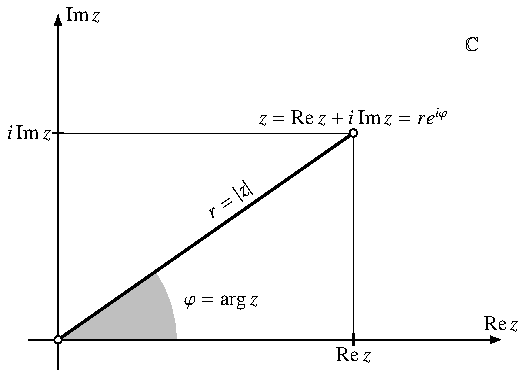
\includegraphics{chapters/a-komplex/gauss.pdf}
\caption{Komplexe Zahlenebene
\label{skript:gaussebene}}
\end{figure}
\index{Gauss-Ebene}%
\index{komplexe Zahlenebene}%

Mit Hilfe der komplexen Konjugation kann man den Real- und Imaginärteil
einer komplexen Zahl $z=a+bi$ direkt ausdrücken:
\begin{align}
\operatorname{Re}z 
&=
a=\frac{(a+bi)+(a-bi)}2=\frac{z+\bar z}2
\label{skript:realteil-formel}
\\
\operatorname{Im}z
&=
b=\frac{(a+bi)-(a-bi)}{2i}=\frac{z-\bar z}{2i}.
\label{skript:imaginaerteil-formel}
\end{align}

\subsection{Polardarstellung}
\index{komplexe Zahl!Polardarstellung}
Die Darstellung der komplexen Zahlen als Punkte einer Ebene suggeriert
auch eine alternative Schreibweise.
Ein Punkt $z$ der komplexen Ebene kann auch charakterisiert werden mit Hilfe von
Polarkoordinaten, also durch seine Entfernung $r=|z|$ vom Nullpunkt,
und durch Polarwinkel zwischen der reellen Achse und der Richtung
zur komplexen Zahl. Der Polarwinkel heisst auch {\em Argument} $\operatorname{arg}z$,
\index{Argument}%
und es gilt
\[
\tan\operatorname{arg}z=\frac{\operatorname{Im}z}{\operatorname{Re}z}.
\]
\index{komplexe Zahl!Argument}
\index{komplexe Zahl!Betrag}
\index{komplexe Zahl!Multiplikation}
Die Multiplikation von komplexen Zahlen bekommt in der Polardarstellung
eine besondere Interpretation:
\begin{align*}
z_1z_2
&=
(r_1\cos\varphi_1+ir_1\sin\varphi_1) (r_2\cos\varphi_2+ir_2\sin\varphi_2)
\\
&=
r_1r_2(\cos\varphi_1+i\sin\varphi_1) (\cos\varphi_2+i\sin\varphi_2)
\\
&=
r_1r_2\bigl(
\cos\varphi_1\cos\varphi_2-\sin\varphi_1\sin\varphi_2 +
(\cos\varphi_1\sin\varphi_2+\sin\varphi_1\cos\varphi_2)i\bigr)
\\
&=
r_1r_2(\cos(\varphi_1+\varphi_2)+i\sin(\varphi_1+\varphi_2))
\\
\Rightarrow \operatorname{arg}z_1z_2&=\arg z_1 + \arg z_2
\end{align*}
Die Multiplikation zweier komplexen Zahlen entspricht also der
Multiplikation der Beträge, und der Addition der Argumente.

Wir versuchen jetzt, die Werte der Exponentialfunktion zu $e^z$ zu
bestimmen.
Die Exponentialgesetze sollten auch weiterhin gelten.
Sei also $z=a+bi$, dann ist
\[
e^z=e^{a+bi}=e^a\cdot e^{bi}.
\]
Die Exponentialfunktion reeller Zahlen ist bereits wohlbekannt, es muss
also nur noch untersucht werden, welche Bedeutung $e^{bi}$ hat.

Betrachten wir die Funktion $f(t)= e^{it}$. Die Ableitungen von $f$ sind
\begin{align}
f'(t)&=ie^{it}=if(t)\notag\\
f''(t)&=-f(t).\label{skript:exp-dgl}
\end{align}
Die Funktion $f$ muss also eine Lösung der Differentialgleichung
\eqref{skript:exp-dgl} sein, welche die Anfangsbedingungen $f(0)=1$ und
$f'(0)=if(0)=i$ erfüllen muss.
Doch die Differentialgleichung \eqref{skript:exp-dgl} hat die Lösungen
\[
f(t)=a\cos t+b\sin t.
\]
Setzt man die Anfangsbedingungen ein, findet man
\begin{align*}
f(0)&=1&\Rightarrow&&a&=1\\
f'(0)&=1&\Rightarrow&&b&=i,
\end{align*}
so dass wir jetzt $e^{it}$ ausrechnen können:
\begin{satz}[Euler]
\begin{align}
e^{it}=\cos t+i\sin t.
\label{skript:euler-formula}
\end{align}
\end{satz}
\index{Euler-Formel}%

Die komplexe Konjugation kehrt das Vorzeichen des Imaginärteils um, also 
von $\sin t$. Da $\sin t$ eine ungerade Funktion ist, ist dies gleichbedeutend
damit, das Vorzeichen von $t$ zu kehren: $\overline{e^{it}}=e^{-it}$.

Mit der Eulerschen Formel sind wir jetzt auch in der Lage, den Zusammenhang
zwischen einer komplexen Zahl und ihrem Betrag und Argument sehr prägnant
auszudrücken:
\[
z=|r|\cdot e^{i\operatorname{arg}z}.
\]
Die Real- und Imaginärteile von $e^{it}$ sind $\cos t$ und $\sin t$,
wir können sie auch mit den Formeln \eqref{skript:realteil-formel} und
\eqref{skript:imaginaerteil-formel} ausdrücken:
\begin{align*}
\cos t
&=
\operatorname{Re}e^{it}
=
\frac{e^{it}+\overline{e^{it}}}2
=
\frac{e^{it}+e^{-it}}2
\\
\sin t
&=
\operatorname{Im}e^{it}=\frac{e^{it}-e^{-it}}{2i}.
\end{align*}

\subsection{Matrixdarstellung der komplexen Zahlen\label{subsection:matrixdarstellung}}
\index{komplexe Zahl!Matrixdarstellung}
Die Algebra der komplexen Zahlen kann man auch als eine Algebra von Matrizen
schreiben. Dazu betrachten wir die Abbildung
\[
\varphi\colon
\mathbb C\to M_2(\mathbb R):
a+bi\mapsto\begin{pmatrix}a&b\\-b&a\end{pmatrix}
\]
Die imaginäre Einheit $i$ wird von $\varphi$ auf die Matrix
\[
\varphi(i)=J=\begin{pmatrix}0&1\\-1&0\end{pmatrix}
\]
abgebildet. Man kann nachrechnen, dass $J^2=-E$, und dass die Rechenregeln
für die komplexen Zahlen durch die Abbildung $\varphi$ in die Rechenregeln
für Matrizen transformiert werden.
Wir illustrieren dies für die Multiplikation:
\[
\begin{aligned}
&(a+bi)(c+di)&&\mapsto&
&\begin{pmatrix}a&b\\-b&a\end{pmatrix}
\begin{pmatrix}c&d\\-d&c\end{pmatrix}
\\
&(ac-bd) + i(ad-bc)&&\mapsto&
&=\begin{pmatrix}
ac-bd&ad-bc\\
-ad+bc&ac-bd
\end{pmatrix}
\end{aligned}
\]
In dieser Darstellung kann man auch $e^{Jt}$ ausrechnen, indem man $Jt$ in
die Taylorreihe von $e^x$ einsetzt
\begin{align}
e^{Jt}
&=
E + tJ + \frac{t^2}{2!} J^2 + \frac{t^3}{3!} J^3 + \frac{t^4}{4!} J^4
 + \frac{t^5}{5!} J^5 + \frac{t^6}{6!} J^6 + \frac{t^7}{7!} J^7 + \dots
\notag
\\
&=
E + tJ - \frac{t^2}{2!} E - \frac{t^3}{3!} J + \frac{t^4}{4!} E
 - \frac{t^5}{5!} J - \frac{t^6}{6!} E + \frac{t^7}{7!} J + \dots
\notag
\\
&=\biggl(1 - \frac{t^2}{2!} + \frac{t^4}{4!} - \frac{t^6}{6!} + \dots\biggr) E
+ \biggl(t - \frac{t^3}{3!} + \frac{t^5}{5!} - \frac{t^7}{7!} + \dots\biggr) J
= E \cos t + J \sin t.
\label{skript:eulermatrixdarstellung}
\end{align}
Die Eulerformel \eqref{skript:euler-formula} lässt sich also auch in der
Matrixdarstellung der komplexen Zahlen wiedergewinnen.

\section{Komplexe Matrizen}
\rhead{Komplexe Matrizen}
\index{Matrix!komplex}%
Die Lineare Algebra im Bachelor wird typischerweise nur in den
reellen Zahlen entwickelt, der einzige untersuchte Vektorraum ist
der Raum $\mathbb R^n$ der reellen $n$-dimensionalen Vektoren.
Für die Quantenmechanik benötigen wir aber auch Vektoren mit
komplexen Komponenten. Der $n$-dimensionale komplexe Vektorraum
$\mathbb C^n$ ist die Menge
\[
\left\{\left.\begin{pmatrix}c_1\\\vdots\\c_n\end{pmatrix}\,\right|
c_i\in\mathbb C\right\},
\]
mit der komponentenweisen Addition und der Multiplikation mit einer
komplexen Zahl. Nichts an der elementaren linearen Algebra hat besondere
Eigenschaften der reellen Zahlen verwendet, die nicht auch die komplexen
Zahlen haben. Der Gauss-Algorithmus, die Konstruktion der Determinanten,
ja sogar der grundlegende Algorithmus zur Lösung des Eigenwertproblems
funktioniert genau gleich auch für komplexe Matrizen. Nur im Bereich
des Skalarproduktes sind minimale Modifikationen notwendig.

\subsection{Skalarprodukt für komplexe Vektorräume}
In der linearen Algebra im ersten Semester wird das Skalarprodukt
geometrisch mit Hilfe der Projektion eingeführt.
Eine solche Konstruktion ist für komplexe Vektoren nicht möglich,
weil es keine anschauliche komplexe Geometrie gibt.

\subsubsection{Komplexes Skalarprodukt}
Um ein komplexes Skalarprodukt zu bekommen, gehen wir daher von den
algebraischen Eigenschaften des Skalarproduktes aus:
\begin{compactenum}
\item Das Skalarprodukt $(u,v)$ von komplexen Vektoren $u$ und $v$ ist linear
in $v$.
\item $(u,u) > 0$ falls $u\ne 0$.
\item Falls $(u,v)\in\mathbb R$, dann ist $(u,v)=(v,u)$.
\end{compactenum}
Diese Eigenschaften müssen auch für ein komplexes Skalarprodukt gelten.
Wir zeigen, dass diese Eigenschaften auch ein komplexes Skalarprodukt 
weitgehend festlegt.

Zunächst stellen wir fest, dass wir nicht erwarten können, dass
ein Skalarprodukt linear sein kann.
Betrachten wir dazu einen eindimensionalen Vektorraum $\mathbb C^1$.
Vektoren sind hier nur komplexe Zahlen, und ein Produkt, welches
linear in beiden Faktoren ist, ist von der Form $(u,v)=uv$. Dann ist
aber $(u,u)=u^2$, aber $u^2$ kann auch negativ sein, zum Beispiel für $u=i$.
Das einzige Produkt, welches immer positiv ist, ist $(u,v)=\bar uv$.
Dieses Produkt ist aber nicht linear im Faktor $u$:
\[
(\lambda u,v)=\overline{(\lambda u)}v=\bar\lambda (\bar uv)=\bar\lambda (u,v).
\]
Wir müssen also von einem komplexen Skalarprodukt verlangen, dass es
\index{konjugiert linear}
im ersten Faktor {\em konjugiert linear} ist:
\[
(\lambda u,v)=\bar\lambda(u,v)
\]
Eine Funktion von zwei Vektoren, welche linear im zweiten Vektor ist
und konjugiert linear im ersten heisst {\em sesquilinear}.
\index{sesquilinear}%
\index{Sesquilinearform}%

Sei jetzt also $(\,\cdot\,|\,\cdot\,)$ eine Sesquilinearform.
Wir setzen $\lambda = 1/(u,v)$, dann gilt
$(u,\lambda v)$ reell ist. Dann gilt
\begin{align*}
1&=\lambda (u,v)=(u,\lambda v)=(\lambda v,u)=\bar\lambda(v,u)
&
&\Rightarrow&
\frac1{(\bar\lambda)}&=(v,u)
&
&\Rightarrow&
\overline{(u,v)}&=(v,u).
\end{align*}
Vertauschung der Faktoren ist also gleichbedeutend mit komplexer Konjugation
des Wertes des Skalarproduktes. Man nennt eine Funktion von zwei komplexen
Vektoren {\em hermitesch}, wenn $(u,v)=\overline{(v,u)}$ gilt.
\index{hermitesch}
\index{Matrix!hermitesch}

Eine hermitesche Sesquilinearform heisst {\em positiv definit}, wenn
\index{positiv definit}
für jeden Vektor $u\ne 0$ gilt $(u,u)>0$. Diese Eigenschaft stellt
sicher, dass $(u,u)$ sinnvoll als die ``Länge'' eines Vektors interpretiert
werden kann.

\begin{definition}
Ein komplexes Skalarprodukt ist eine positiv definite,
hermitesche Sesquilinearform.
\end{definition}
\index{Skalarprodukt!komplexes}

Das einfachste Beispiel eines komplexen Skalarproduktes ist
\[
(u,v)=\sum_i \bar u_iv_i.
\]
Die Standardbasisvektoren sind auch in diesem Skalarprodukt
orthonormiert.

%
% Adjungierte Matrix
%
\subsubsection{Adjungierte Matrix}
\index{adjungiert}
\index{Matrix!adjungiert}
\index{Abbildung!linear}
In den reellen Vektorräumen konnte man zu einer linearen $A$ immer
eine lineare Abbildung $A^t$ finden mit der Eigenschaft
$(u,Av)=(A^tu,v)$. Mit Hilfe der Standardbasisvektoren konnte
man auch ausrechnen, was dies für die Matrizen von $A$ bedeutet:
\[
(e_i,A^te_j),
=
(A^te_j, e_i)
=
(e_j,Ae_i)=a_{ji}
\]
d.~h.~die Matrix von $A^t$ ist die transponierte Matrix von $A$.
Eine symmetrische Matrix war eine, die sich beim Transponieren nicht
ändert, also $A^t=A$.

Dasselbe kann man jetzt auch für ein komplexes Skalarprodukt
versuchen. Zu einer komplexen Matrix $A$ ist also eine neue
Matrix $A^*$ gesucht, mit der Eigenschaft, $(A^*u,v)=(u,Av)$ für 
jedes Paar von Vektoren $u$ und $v$. Für die Standardbasisvektoren
gilt dann
\[
(e_i,A^*e_j),
=
\overline{(A^*e_j, e_i)}
=
\overline{(e_j,Ae_i)}=\overline{a_{ji}},
\]
die Matrix von $A^*$ ist also nicht nur transponiert, sondern auch komplex
konjugiert. Hat $A$ die Ma\-trix\-e\-le\-men\-te $a_{ij}$ dann nennt man
die Matrix $A^*$ mit den Matrixelementen $\bar a_{ji}$ die
adjungierte Matrix. Eine Matrix, die sich beim Adjungieren nicht
ändert, heisst {\em selbstadjungiert}.
\index{Matrix!selbstadjungiert}
\index{selbstadjungiert}

Die Rechenregeln für die adjungierte Matrix sind ganz ähnlich wie
für die Transposition:
\index{Transposition}%
\[
\begin{aligned}
(\lambda A)^*&=\bar\lambda A^*,
&
(A+B)^*&=A^*+B^*,
&
(AB)^*=B^*A^*.
\end{aligned}
\]
Man beachte, dass $A\mapsto A^*$ nicht linear ist.

\subsubsection{Unitäre Matrizen}
\index{unitar@unitär}
Matrizen, die in reellen Vektorräumen das Skalarprodukt nicht ändern,
heissen orthogonal. Sie sind charakterisiert durch die Eigenschaft
\index{Matrix!orthogonal}%
\index{orthogonal}%
$(Ox,Oy)=(x,y)$, woraus sich mit Hilfe der Transposition ergibt:
\[
(Ox,Oy)=(O^tOx,y)=(x,y)\qquad\Rightarrow\qquad O^tO=E,
\]
woraus man weiter ablesen kann, dass bei orthogonalen Matrizen
die transponierte Matrix mit der invertierten Matrix zusammenfällt.

Für komplexen Vektoren kann man wieder nach den Matrizen fragen, die das
komplexe Skalarprodukt nicht verändern. Eine Matrix $U$ hat diese
Eigenschaft, wenn
\[
(Ux,Uv)=(U^*Ux,y)=(x,y)\;\forall x,y
\qquad\Rightarrow\qquad
U^*U=E
\]
gilt,
eine solche Matrix heisst {\em unitär}. 
\index{unitar@unitär}
\index{Matrix!unitär}

Für reelle Matrizen $A$ ist $A^t=A^*$, also sind orthogonale Matrizen
auch unitär.

\begin{beispiel}
Die unitären $1\times 1$-Matrizen sind komplexe Zahlen $z$, welche
die zusätzliche Bedingung $\bar zz=1$ erfüllen müssen.
Die Menge der unitären $1\times 1$-Matrizen ist also
\[
U(1)=\left\{ z\in\mathbb C\,|\, |z|=1
\right\}.
\]
In der Quantenmechanik können Zustandsvektoren in der Regel nur bis auf
einen komplexen Faktor vom Betrag $1$, also bis auf ein Element
von $U(1)$ festgelegt werden.
Man spricht oft von ``bedeutungslosen'' Phasenfaktoren.
\end{beispiel}

\subsubsection{Die spezielle unitäre Gruppe $\operatorname{SU}(2)$}
\index{spezielle unitäre Gruppe}
\index{SU(2)}
Wir betrachten Matrizen der Form
\begin{equation}
U=
\begin{pmatrix}
a&b\\-\bar b&\bar a
\end{pmatrix}
\label{skript:su2form}
\end{equation}
mit der zusätzlichen Bedingung $|a|^2 + |b|^2=1$. Sie erfüllen
\begin{align*}
U^*U
&=
\begin{pmatrix}
\bar a&-b\\\bar b&a
\end{pmatrix}
\begin{pmatrix}
a&b\\-\bar b&\bar a
\end{pmatrix}
=
\begin{pmatrix}
\bar aa+b\bar b & \bar ab-b\bar a\\
\bar ba-a\bar b & \bar bb+a\bar a
\end{pmatrix}
=
E
\\
\det(U)&=\left|
\begin{matrix}
a&b\\-\bar b&\bar a
\end{matrix}
\right|
=
a\bar a+\bar bb = |a|^2 + |b|^2=1.
\end{align*}
Solche Matrizen sind also nicht nur unitär, sondern haben auch Determinante 1.
Multipliziert man zwei Matrizen der Form \eqref{skript:su2form},
wird das Produkt auch wieder Determinante 1 haben, aber es ist nicht klar,
dass es sich in der Form \eqref{skript:su2form} schreiben lässt.
Daher rechnen wir das Produkt aus, wir erhalten
\begin{align*}
\begin{pmatrix}  a                        & b                      \\
                 -\bar b                  & \bar a                 \end{pmatrix}
\begin{pmatrix}  c                        & d                      \\
                 -\bar d                  & \bar c                 \end{pmatrix}
&=
\begin{pmatrix}  ac-b\bar d               & ab+b\bar c             \\
                 -\bar bc-\bar a\bar d    & -\bar bd +\bar a\bar c \end{pmatrix}
=
\begin{pmatrix}  ac-b\bar d               & ab+b\bar c             \\
                 -(\overline{ab+b\bar c}) & \overline{ac-b\bar d}  \end{pmatrix}
.
\end{align*}
Das Produkt zweier Matrizen der Form \eqref{skript:su2form} ist also wieder eine
Matrix der Form \eqref{skript:su2form}.
Die Menge dieser Matrizen ist demzufolge abgeschlossen unter
Matrixmultiplikation und Bildung der Inversen.
Man nennt diese Matrizen die Gruppe der speziellen unitären Matrizen:
\[
\operatorname{SU}(2)=\left\{
\left.
\begin{pmatrix}
a&b\\-\bar b&\bar a
\end{pmatrix}
\,
\right|
\,
a,b\in\mathbb C\wedge
|a|^2+|b|^2=1
\right\}.
\]
Die Gruppe $\operatorname{SU}(2)$ spielt bei der Analyse des Elektronenspins
eine wichtige Rolle.

Die Gruppe $\operatorname{SU}(2)$ ist eine Teilmenge der Menge der komplexen
$2\times 2$-Matrizen:
\[
\operatorname{SU}(2)
\subset
V=
\left\{
\left.
\begin{pmatrix}a&b\\-\bar b&\bar a\end{pmatrix}\,
\right|
a,b\in\mathbb C^2
\right\}
\subset
M_2(\mathbb C)
=\left\{
\left.
\begin{pmatrix}
a&b\\c&d
\end{pmatrix}
\,
\right|
\, a,b,c,d\in\mathbb C
\right\}
\]
Wir untersuchen die Menge $V$ etwas genauer.
Zunächst können wir $V$ als zweidimensionalen komplexen Vektorraum
betrachten wie $\mathbb C^2$.
Als reeller Vektorraum betrachtet ist $V$ ein vierdimensionaler
reeller Vektorraum. Die Abbildung
\[
\mathbb R^4\to\mathbb C^2\to V
:
\begin{pmatrix}x_1\\x_2\\x_3\\x_4\end{pmatrix}\mapsto
\begin{pmatrix}x_1+ix_2\\x_3+ix_4\end{pmatrix}\mapsto
\begin{pmatrix} x_1+ix_2 & x_3+ix_4 \\
               -x_3+ix_4 & x_1-ix_2 \end{pmatrix}
\]
ist eine Bijektion zwischen $\mathbb R^4$, $\mathbb C^2$ und $V$.
Auch geometrisch ist $\mathbb C^2=\mathbb C\times \mathbb C$ das Produkt
von zwei Ebenen, hat also eine vierdimensionale Geometrie.
Darin ist $\operatorname{SU}(2)$ die Teilmenge der vierdimensionalen Vektoren,
und zwar derjenigen für die gilt
\[
1
=
|a|^2+|b|^2
= 
x_1^2 + x_2^2 + x_3^2 + x_4^2,
\]
das sind die Vektoren von $\mathbb R^4$ mit Länge $1$.
Geometrisch ist $\operatorname{SU}(2)$ also eine dreidimensionale Kugel
eingebettet in in einen vierdimensionalen Raum.

\subsubsection{Spur und Determinante}
\index{Spur}%
\index{Determinante}%
Spur und Determinate können samt all ihren Rechenregeln sofort auf
komplexe Matrizen übertragen werden.
Für den Adjunktionsoperator finden wir die Rechenregeln
\[
\begin{aligned}
\det A^*&= \overline{\det A^t}=\overline{\det A},
&&\text{und}&
\operatorname{tr} A^*&=\overline{\operatorname{tr}A}.
\end{aligned}
\]
Für selbstadjungierte Matrizen kann man schliessen, dass sowohl
die Determinante wie auch die Spur von $A$ reell sein müssen.

In den komplexen Zahlen hat jedes Polynom $n$-ten Grades $n$ Nullstellen.
Daher können wir das charakteristische Polynom immer ausschreiben als
\begin{align*}
\det(A-\lambda E)
&=
(-1)^n (\lambda-\lambda_1)\dots(\lambda-\lambda_n)
\\
&=
(-1)^n(\lambda^n -(\lambda_1+\dots+\lambda_n)\lambda^{n-1}+\dots
+(-1)^n\lambda_1\dots\lambda_n
\\
&=
(-1)^n(\lambda^n - \operatorname{tr}A\lambda^{n-1}+\dots + (-1)^n\det A)
\end{align*}
Daraus können wir auch eine Formel für $\det(E+tA)$ ableiten:
\begin{align}
\det(E+tA)
&=
(-t)^n\det\biggl(A-\frac1tE\biggr)
=
t^n\biggl(
\frac1{t^n}+\frac1{t^{n-1}}\operatorname{tr}A+\dots+\det A
\biggr)
\notag
\\
&=
1+t\operatorname{tr}A+\dots+t^n\operatorname{det}A
\label{skript:detandtrace}
\end{align}

%
% Eigenwertproblem fuer komplexe Matrizen
%
\subsection{Eigenwertproblem für komplexe Matrizen}
\subsubsection{Definition}
Ein Vektor $v\ne 0$ heisst {\em Eigenvektor zum Eigenwert} $\lambda$ einer
\index{Eigenwert}
\index{Eigenvektor}
Matrix $A$, wenn $Av=\lambda v$ gilt. Diese Definition ist auch für
komplexe Matrizen gültig, ebenso funktioniert der Standardalgorithmus
für die Lösung des Eigenwertproblems nach wie vor:
\begin{enumerate}
\item Finde die Nullstellen der charakteristischen Gleichung
$\det(A-\lambda E)=0$.
\item Für jede Nullstelle $\lambda_i$, finde Eigenvektoren
durch Lösung des Gleichungssystems $(A-\lambda_i E)v=0$.
\end{enumerate}
Der wesentliche Unterschied ist jedoch, dass in den komplexen
Zahlen ein Polynom vom Grade $n$ immer $n$ Nullstellen hat.
Die bei reellen Matrizen vorkommende Situation, dass weniger
als $n$ reelle Nullstellen existieren, und daher nicht genügend
Eigenvektoren für eine Eigenvektorbasis gefunden werden können,
tritt also bei komplexen Matrizen seltener auf.

\subsubsection{Selbstadjungierte Matrizen}
Der quantenmechanische Formalismus beschreibt physikalische Grössen
als selbstadjungierte Matrizen. Die möglichen Werte einer solchen Grösse
sind die Eigenwerte der Matrix, und es muss sichergestellt werden,
dass keine komplexen Eigenwerte auftreten können.

\begin{satz}
\label{skript:ewreell}
Die Eigenwerte einer selbstadjungierten Matrix sind reell.
\end{satz}
\begin{proof}[Beweis]
Sei $v$ ein Eigenvektor zum Eigenwert $\lambda$ einer selbstadjungierten
Matrix $A$. Dann gilt
\begin{align*}
(v,Av)
&=
\lambda(v,v)
\\
&=(Av,v)=(\lambda v,v)=\bar\lambda(v,v)
\\
\Rightarrow \lambda&=\bar\lambda,
\end{align*}
also ist $\lambda\in\mathbb R$.
\end{proof}

Bei reellen Matrizen hat sich gezeigt, dass symmetrische Matrizen immer
diagonalisierbar sind. Dies gilt auch für selbstadjungierte Matrizen
in komplexen Vektorräumen:

\begin{satz}
\label{skript:evorthogonal}
Eine selbstadjungierte Matrix ist diagonalisierbar und die Eigenvektoren zu
verschiedenen Eigenwerten sind orthogonal.
\end{satz}

\begin{proof}[Beweis]
Wir beweisen nur die Orthogonalität von Eigenvektoren zu verschiedenen 
Eigenwerten. Seien also $v_1,v_2$ Eigenvektoren zu zwei verschiedenen
Eigenwerten $\lambda_1,\lambda_2$. Die beiden Eigenwerte sind nach
Satz~\ref{skript:ewreell} reell. Dann gilt
\begin{align*}
(v_1,Av_2)&=\lambda_2(v_1,v_2)
\\
          &=(Av_1,v_2)=\bar\lambda_1(v_1,v_2)=\lambda_1(v_1,v_2)
\\
\Rightarrow\quad
(\lambda_1-\lambda_2)(v_2,v_2)&=0
\end{align*}
Die letzte Gleichung kann wegen $\lambda_1\ne\lambda_2$ nur wahr sein,
wenn $(v_1,v_2)=0$, die Vektoren $v_1$ und $v_2$ müssen also orthogonal sein.
\end{proof}

%
% Lie Algebrean
%
\section{Lie-Algebren}
\rhead{Lie-Algebren}
\index{Lie-Algebra}
Die invertierbaren Matrizen $\operatorname{GL}(n)$ können weiter
unterteilt werden in invertierbare Matrizen mit zusätzlichen
Eigenschaften wie Orthogonalität oder spezielle Werte der Determinanten.
Allerdings bildet die Menge der invertierbaren Matrizen keinen
Vektorraum: man kann sie nicht addieren oder mit beliebigen Zahlen
multiplizieren, weil die Invertierbarkeit oder eine der zusätzlichen
Eigenschaften dabei verloren gehen kann. Diese Matrizen sind 
daher nicht geeignet als Observable in der Quantenmechanik.

Ist eine Matrix $A$ invertierbar, dann wird auch eine Matrix, deren
Matrixelemente nur wenig von $A$ abweichen, invertierbar sein.
Insbesondere werden die Matrizen der Form $E+tA$ invertierbar sein,
wenn nur $t$ klein genug ist. Dies ist ein Übergang zu einer 
infinitesimalen Transformation $A$.

Wie müssen die Rechenoperationen beim Übergang zu infinitesimalen
Transformationen übersetzt werden?
Wegen
\[
(E+tA)(E+tB)=E+(A+B)t + t^2AB\simeq E+(A+B)t
\]
wird beim Übergang zur infinitesimalen Transformation aus dem Produkt
der Matrizen die Summe von Matrizen, und aus der Inversen wird die Negation.

Betrachten wir die Bedingung Orthogonalität
\[
E=
(E+\varepsilon A)^t(E+\varepsilon A)
=
E+\varepsilon (A^t+A) + \dots
\qquad
\Rightarrow
\qquad
A^t=-A.
\]
Die infinitesimale Versionen von orthogonalen Matrizen sind also
antisymmetrische Matrizen.
\index{antihermitesche Matrix}
\index{Matrix!antihermitesch}
Analog sind die infinitesimalen Versionen von unitären Matrizen
antihermitesch.

Die Matrizenmultiplikation ist nicht kommutativ.
Diese Tatsache kann ausgenutzt werde, um den
Matrizenmengen eine zusätzliche algebraische Struktur zu geben.
\index{Kommutator}%
Der Kommutator $[A,B]=AB-BA$ zweier Matrizen $A$ und $B$ erhält
die oben genannten Eigenschaften. Ist $A$ antisymmetrisch, dann
ist auch $[A,B]$ auch antisymmetrisch:
\[
[A,B]^t
=
(AB-BA)^t
=
B^tA^t-A^tB^t
=
(-B)(-A)-(-A)(-B)
=
-(AB-BA)
=
-[A,B].
\]
\index{Jacobi-Identität!für Operatoren}%
Die Kommutatorklammer hat aber auch noch eine zusätzliche Eigenschaft,
für drei Matrixen $A$, $B$ und $C$ gilt nämlich die sogenannte
Jacobi-Identität:
\begin{equation}
[A,[B, C]]
+
[B,[C, A]]
+
[C,[A, B]]
=
0
\label{skript:jacobi}
\end{equation}
Um dies einzusehen rechnen wir die Kommutatoren aus:
\begin{align*}
&
[A,[B, C]]
+
[B,[C, A]]
+
[C,[A, B]]
\\
&=
A(BC-CB)-(BC-CB)A
+
B(CA-AC)-(CA-AC)B
+
C(AB-BA)-(AB-BA)C
\\
&=
ABC-ACB-BCA+CBA
+
BCA-BAC-CAB+ACB
+
CAB-CBA-ABC+BAC
\\
&=0
\end{align*}
Ein Vektorraum mit einer antisymmetrischen, bilinearen Abbildung
$[\,\cdot\,,\,\cdot\,]$,
welche die Jacobi-Identität \eqref{skript:jacobi} erfüllt, heisst eine
{\em Lie-Algebra}.
\index{Lie-Algebra}%
So wie der Hamilton-Operator als Erzeuger der Zeitentwicklung das
leichter zu manipulierende Objekt ist, ist die Liealgebra zu einer
Transformationsgruppe wie $\operatorname{SU}(2)$ besser geeignet
zur Beschreibung von Transformationen, und wird daher von Physikern
vorgezogen.

\begin{beispiel}
\index{SO(3)}
Zur Gruppe $\operatorname{SO}(3)$ der Drehmatrizen gehört die Lie-Algebra
$\operatorname{so}(3)$ der antisymmetrischen $3\times 3$-Matrizen.
\index{Drehmatrix}%
Solche Matrizen haben die Form
\[
\Omega
=
\begin{pmatrix}
    0    & \omega_3&-\omega_2\\
-\omega_3&   0     & \omega_1\\
 \omega_2&-\omega_1&    0
\end{pmatrix}
\]
Der Vektorraum $\operatorname{so}(3)$ ist also dreidimensional.

Die Wirkung von $E+t\Omega$ auf einem Vektor $x$ ist
\[
(E+t\Omega)
\begin{pmatrix}x_1\\x_2\\x_3\end{pmatrix}
=
\begin{pmatrix}
    1     & t\omega_3&-t\omega_2\\
-t\omega_3&   1      & t\omega_1\\
 t\omega_2&-t\omega_1&    1
\end{pmatrix}
\begin{pmatrix}x_1\\x_2\\x_3\end{pmatrix}
=
\begin{pmatrix}
x_1-t(-\omega_3x_2+\omega_2x_3)\\
x_2-t( \omega_3x_1-\omega_1x_3)\\
x_3-t(-\omega_2x_1+\omega_1x_2)
\end{pmatrix}
=
x- t\begin{pmatrix}\omega_1\\\omega_2\\\omega_3\end{pmatrix}\times x
=
x+ tx\times \omega.
\]
Die Matrix $\Omega$ ist als die infinitesimale Version einer Drehung
um die Achse $\omega$.

Wir können die Analogie zwischen Matrizen in $\operatorname{so}(3)$ und
Vektoren in $\mathbb R^3$ noch etwas weiter treiben. Zu jedem Vektor
in $\mathbb R^3$ konstruieren wir eine Matrix in $\operatorname{so}(3)$
mit Hilfe der Abbildung
\[
\mathbb R^3\to\operatorname{so}(3)
:
\begin{pmatrix}v_1\\v_2\\v_3\end{pmatrix}
\mapsto
\begin{pmatrix}
  0 & v_3&-v_1\\
-v_3&  0 & v_2\\
 v_1&-v_2&  0
\end{pmatrix}.
\]
Der Kommutator von zwei so aus Vektoren $\vec u$ und $\vec v$
konstruierten Matrizen $U$ und $V$ ist:
\begin{align*}
[U,V]
&=
UV-VU
\\
&=
\begin{pmatrix}
  0 & u_3&-u_1\\
-u_3&  0 & u_2\\
 u_1&-u_2&  0
\end{pmatrix}
\begin{pmatrix}
  0 & v_3&-v_1\\
-v_3&  0 & v_2\\
 v_1&-v_2&  0
\end{pmatrix}
-
\begin{pmatrix}
  0 & v_3&-v_1\\
-v_3&  0 & v_2\\
 v_1&-v_2&  0
\end{pmatrix}
\begin{pmatrix}
  0 & u_3&-u_1\\
-u_3&  0 & u_2\\
 u_1&-u_2&  0
\end{pmatrix}
\\
&=
\begin{pmatrix}
u_3v_3+u_1v_1 - u_3v_3 - u_1v_1
	& u_1v_2 - u_2v_1
		& u_3v_2 - u_2v_3 
\\
u_2v_1 - u_1v_2
	& -u_3v_3-u_2v_2 + u_3v_3+u_2v_2
		& u_3v_1 - u_1v_3
\\
u_2v_3 - u_3v_2         
	& u_1v_3 - u_3v_1
		&-u_1v_1-u_2v_2 u_1v_1+u_2v_2
\end{pmatrix}
\\
&=
\begin{pmatrix}
0
	& u_1v_2 - u_2v_1
		&-(u_2v_3-u_3v_2)
\\
-( u_1v_2 - u_2v_1)
	& 0
		& u_3v_1 - u_1v_3
\\
u_2v_3 - u_3v_2         
	&-( u_3v_1 - u_1v_3)
		& 0
\end{pmatrix}
\end{align*}
Die Matrix $[U,V]$ gehört zum Vektor $\vec u\times\vec v$.
Damit können wir aus der Jacobi-Identität jetzt folgern, dass
\[
\vec u\times(\vec v\times w)
+
\vec v\times(\vec w\times u)
+
\vec w\times(\vec u\times v)
=0
\]
für drei beliebige Vektoren $\vec u$, $\vec v$ und $\vec w$ ist.
Dies bedeutet, dass der dreidimensionale Vektorraum $\mathbb R^3$
mit dem Vektorprodukt zu einer Lie-Algebra wird.
In der Tat verwenden einige Bücher statt der vertrauten Notation
$\vec u\times \vec v$ für das Vektorprodukt die aus der Theorie der
Lie-Algebren entlehnte Notation $[\vec u,\vec v]$, zum Beispiel
das Lehrbuch der Theoretischen Physik \cite{skript:landaulifschitz1}
von Landau und Lifschitz.

Die Lie-Algebren sind vollständig klassifiziert worden, es gibt
keine nicht trivialen zweidimensionalen Lie-Algebren.
Unser dreidimensionaler Raum ist also auch in dieser Hinsicht speziell:
es ist der kleinste Vektorraum, in dem eine nichttriviale Lie-Algebra-Struktur
möglich ist.
\end{beispiel}

\begin{beispiel}
Die Gruppe $\operatorname{SU}(2)$ hat als infinitesimale Erzeugende 
die antihermiteschen Matrizen, also Matrizen mit der Eigenschaft
\[
A^*=-A,
\qquad
\Rightarrow
\qquad
\begin{pmatrix}
   ia&b+ic\\
-b+ic&  id
\end{pmatrix}.
\]
Darin wurde aber die Bedingung noch nicht abgebildet, dass Matrizen
in $\operatorname{SU}(2)$ die Determinante $1$ haben müssen, wir
haben bis jetzt nur Unitarität verwendet. Wir müssen also noch
verlangen, dass in erster Näherung $\det(E+tA)=0$ ist.
Aus Formel \eqref{skript:detandtrace} schliessen wir, dass die Spur
$\operatorname{tr}A$ verschwindet, oder dass $a=-d$:
\begin{equation}
\operatorname{su}(2)
=
\left\{ A\in M_2(\mathbb C)\,|\,
A^*=-A\wedge \operatorname{tr}A=0
\right\}
\end{equation}
Matrizen in $\operatorname{su}(2)$ haben also die Form
\begin{equation}
\begin{pmatrix}
   ia&b+ic\\
-b+ic& -ia
\end{pmatrix},\qquad a,b,c\in\mathbb R
\end{equation}
Die Menge $\operatorname{su}(2)$ ist also eine dreidimensionale 
Lie-Algebra.
Als Basis von $\operatorname{su}(2)$ können die Matrizen
\begin{align}
I
&=
\begin{pmatrix} 0&1 \\ -1& 0 \end{pmatrix},
&
J
&=
\begin{pmatrix} 0&i \\  i& 0 \end{pmatrix},
&
K
&=
\begin{pmatrix} i&0 \\  0&-i \end{pmatrix}
\label{skript:komplex:definitionIJK}
\end{align}
verwendet werden.
Die Matrix $I$ kennen wir schon von der Matrixdarstellung der komplexen
Zahlen in Abschnitt~\ref{subsection:matrixdarstellung}.
Die Matrizen $I$, $J$ und $K$ haben die folgenden algebraischen
Eigenschaften:
\begin{align*}
I^2
&=
-E
&
IJ
&=
\begin{pmatrix} 0&1 \\ -1& 0 \end{pmatrix}
\begin{pmatrix} 0&i \\  i& 0 \end{pmatrix}
=
\begin{pmatrix} i&0 \\  0&-i \end{pmatrix}
=
K
&
JI
&=
-K
\\
J^2
&=
-E
&
JK
&=
\begin{pmatrix} 0&i \\  i& 0 \end{pmatrix}
\begin{pmatrix} i&0 \\  0&-i \end{pmatrix}
=
\begin{pmatrix} 0&1 \\ -1& 0 \end{pmatrix}
=
I
&
KJ
&=
-I
\\
K^2
&
-E
&
KI
&=
\begin{pmatrix} i&0 \\  0&-i \end{pmatrix}
\begin{pmatrix} 0&1 \\ -1& 0 \end{pmatrix}
=
\begin{pmatrix} 0&i \\  i& 0 \end{pmatrix}
=
J
&
IK
&=
-J
\end{align*}
\index{Quaternionen}%
Dies ist die Algebra der Quaternionen.
\end{beispiel}

Eigentlich hätten wir die Bedingung, dass die Spur verschwinden muss,
schon bei den orthogonalen Matrizen fordern müssen.
Doch antisymmetrische Matrizen haben $0$ auf der Diagonalen, also haben
antisymmetrische Matrizen immer Spur $0$, die Bedingung ist also
automatisch erfüllt.
Antihermitesche Matrizen haben jedoch nicht nur $0$ auf der Diagonalen,
sondern rein imaginäre Zahlen.

\section*{Übungsaufgaben}
\rhead{Übungsaufgaben}
\uebungsaufgabe{15001}
\uebungsaufgabe{15002}
\uebungsaufgabe{15003}
\uebungsaufgabe{15004}
\uebungsaufgabe{15005}
\uebungsaufgabe{15006}

\end{appendices}
\vfill
\pagebreak
\ifodd\value{page}\else\null\clearpage\fi
\lhead{Literatur}
\rhead{}
\printbibliography[heading=subbibliography]
\label{buch:literatur}
\end{refsection}




%
% part2.tex -- format the second part
%
\part{Anwendungen und Weiterführende Themen}
\lhead{Anwendungen}
%
% uebersicht.tex -- Uebersicht ueber die Seminar-Arbeiten
%
% (c) 2018 Prof Dr Andreas Mueller, Hochschule Rapperswil
%
\chapter*{Übersicht}
\lhead{Übersicht}
\rhead{}
\label{buch:uebersicht}
Im zweiten Teil kommen die Teilnehmer des Seminars selbst zu Wort.
Die im ersten Teil dargelegten mathematischen Methoden und
grundlegenden Modelle werden dabei verfeinert, verallgemeinert
und auch numerisch überprüft.






\def\chapterauthor#1{{\large #1}\bigskip\bigskip}
% einzelne Artikel 
%
% addpapers.tex -- file to add all paper main files
%
% (c) 2019 Prof Dr Andreas Müller, Hochschule Rapperswil
%
%
% main.tex -- Paper zum Thema wwt
%
% (c) 2019 Michael Schmid, Hochschule Rapperswil
%
\chapter{Wetter-Wavelet-Transformation\label{chapter:wwt}}
\lhead{Wetter-Wavelet-Transformation}
\begin{refsection}
\chapterauthor{Michael Schmid}



\definecolor{codegreen}{rgb}{0,0.6,0}
\definecolor{codegray}{rgb}{0.5,0.5,0.5}
\definecolor{codepurple}{rgb}{0.58,0,0.82}
\definecolor{backcolour}{rgb}{0.95,0.95,0.92}

\lstdefinestyle{mystyle}{
	backgroundcolor=\color{backcolour},   
	commentstyle=\color{codegreen},
	keywordstyle=\color{magenta},
	numberstyle=\tiny\color{codegray},
	stringstyle=\color{codepurple},
	basicstyle=\footnotesize,
	breakatwhitespace=false,         
	breaklines=true,                 
	captionpos=b,                    
	keepspaces=true,                 
	numbers=left,                    
	numbersep=2pt,                  
	showspaces=false,                
	showstringspaces=false,
	showtabs=false,                  
	tabsize=2
}
\lstset{style=mystyle}
\lstdefinestyle{mystyle}{
	morekeywords={cwt,contourf,datetick}
}


\section{Einführung}
\rhead{Einführung}


Seit Langem konsultiere ich meine aktuellen Wetterdaten über eine eher unübliche Internetseite.
Dabei handelt es sich um eine privat geführte Wetterstation, welche die gemessenen Daten im Internet grafisch darstellt.
Die Daten werden auch tabellarisch zur Verfügung gestellt.
Das Feature, welches ich bis anhin am regelmässigsten nutzte, war die grafische Darstellung der aktuellen Wetterdaten über den Zeitraum der letzten 24 Stunden.
Bei speziellen Ereignissen im Wetterverlauf fielen mir besondere und wiederkehrende Charakteristiken auf.
\\

Nach der Einführung in die Theorie der Wavelets kam mir die Idee, solche Wetterphänomene mit einer geeigneten Wavelet Transformation zu detektieren.
In diesem Paper wird einerseits auf die theoretischen Grundlagen der angewandten Methoden zurückgegriffen sowie die besprochenen meteorologischen Phänomene kurz erläutert. 
Weiterführend wird auf die verwendeten Methoden, auch in der praktischen Anwendung, vertieft eingegangen.
Ein besonderes Augenmerk wird auf die allgemeine Vorgehensweise sowie deren Schwierigkeiten gelegt.
\\




\section{Wetterstation Seegräben}
\rhead{Wetterstation Seegräben}

Die angesprochene Wetterstation in der Gemeinde Seegräben im Kanton Zürich ist mit einer DAVIS Vantage Pro2 6153 \cite{online:davisinstruments} realisiert worden.
Sie verfügt über Sensoren für die Temperatur, Feuchtigkeit, Geschwindigkeit und Richtung des Windes sowie für den Niederschlag. 
Durch diese Sensoren werden folgende Daten aufgezeichnet:


\begin{itemize}
	\item \textbf{Aussentemperatur} in Grad Celsius
	\item \textbf{Relative Luftfeuchtigkeit} in Prozent
	\item \textbf{Luftdruck} in hPa
	\item \textbf{Windgeschwindigkeit} in km/h, gemittelt über 5 Minuten
	\item \textbf{Windböen} in km/h
	\item \textbf{Windrichtung} nach Himmelsrichtung
	\item \textbf{Regenmenge} in $\text{l/m}^{2}$
\end{itemize}	


Der Thermo- / Feuchtigkeitssensor liegt zusammen mit dem Regenmengenmesser auf 2 Meter über Boden.
Mit einem Abstand von rund 10 Meter zum nächsten Gebäude sind optimale Messbedingungen geschaffen.
Mit einem Mast ist der Windmesser auf 1.5 Meter über dem First eines Gebäudes lokalisiert \space \cite{online:wss}.
Die Daten werden anschliessend mit einer Software von PC-Wetterstation.de weiterverarbeitet und auf der Website \cite{online:wss} veröffentlicht.
Mehr zur Verwendung der Wetterdaten im n\"achsten Abschnitt.

\section{Datenaufarbeitung}
\rhead{Datenaufarbeitung}
Der n\"achste Vorbereitungsschritt zur Wavelet Transformation war die Aufbereitung der zur Verf\"ugung gestellten Daten der Wetterstation. Dazu musste erst analysiert werden, wie die Daten auf der Website dargestellt werden.
\subsection{Wetter-Archiv}
Auf der Website gibt es mehrere Möglichkeiten, sich Wetterdaten aus der Vergangenheit darstellen zu lassen.
In der Kategorie des Archivs auf der Website kann man die Wetterdaten eines gew\"unschten Zeitraums tabellarisch oder grafisch darstellen lassen.
Vom Betreiber der Website steht keine Funktion zur Verfügung, welche es erlaubt, die Daten offiziell und automatisch herunterzuladen.
\subsection{Datenerfassung}
Da f\"ur die angestrebte Anwendung eine m\"oglichst hohe Aufl\"osung der jeweiligen Daten erforderlich ist, mussten die Daten im Zeitraum von einem Tag dargestellt werden.
Dies hatte zur Folge, dass man f\"ur jeden Tag eine Tabelle auf dem Archiv der Website \"offnen musste. Man hätte anschliessend die Daten mit copy and paste in eine Excel-Tabelle einf\"ugen können. Daher wurde  entschieden, ein Programm zu schreiben, welches diese Aufgabe automatisieren sollte.
Als Programmiersprache wurde hierf\"ur Python gewählt.


Mit der Pandas Library und der Funktion \texttt{'read\_html'} \space konnten die Daten direkt aus dem Python Programm von der Website heruntergeladen werden.
Entscheidend für das Gelingen dieser Teilaufgabe war, dass die URL-Links der einzelnen Tage stets regelmässig aufgebaut sind:
\\
\\
$$\centering{\textit{https://www.wetter-seegraeben.ch/uploads/insert.php?insert=\textbf{20190701}.htm}}$$
\\
Wie zu sehen ist, wird der Link mit dem Datum regelmässig aufgebaut. Somit konnten die entsprechenden Links mit mehreren While-Schleife zusammengesetzt werden.
In der Abbildung \ref{fig:python-code} ist der wesentliche Ausschnitt aus dem Python Code dargestellt.
\begin{figure}
	\centering
	\lstinputlisting[language=Python,firstline=1,lastline=16,numbers=left,style = Python]{papers/wwt/code/get_data.py}
	\caption{Python Codeausschnitt}
	\label{fig:python-code}
\end{figure}
Die Daten konnten im nächsten Schritt in einer Excel-Tabelle abgespeichert werden.
Dort folgte der letzte Feinschliff; d.h. alle überflüssigen Kopfzeilen und Statistiken wurden entfernt.

\subsubsection{Unregelmässigkeiten der Wetterstation}
Bei der Datenerfassung durch das eben beschriebene Python Programm wurden einige Unregelmässigkeiten der Wetterstation beobachtet.
Das Programm wird jeweils durch eine Fehlermeldung abgebrochen, wenn der angegebene Link nicht abrufbar ist. 
So fiel auf, dass unregelmässig auf das Jahr verteilt, Daten von gewissen Tagen fehlten. Es stellte sich heraus, dass hinter dem eigentlich korrektem Link die entsprechende Internetseite nicht zur Verfügung steht.
Wird manuell auf der Website nach diesem Tag gesucht, kann nichts gefunden werden.
Dies trat teilweise sogar in Abschnitten von mehreren Tagen auf.
Wie sich später herausstellte, traten die fehlenden Tagen nicht zu den Zeitpunkten auf, die mich interessierten.


\subsection{Datendarstellung}
Die Darstellung der gewonnenen Daten konnte einfach mittels Python realisiert werden.
Anbei in Abbildung \ref{fig:rawdata} der Plot der Rohdaten aus dem Jahre 2018, wobei nur jeder zehnte Messpunkt verwendet wurde.
Diese Rohdaten dienten als Grundlage für alle weiteren Berechnungen. 
\begin{figure}
	\centering
	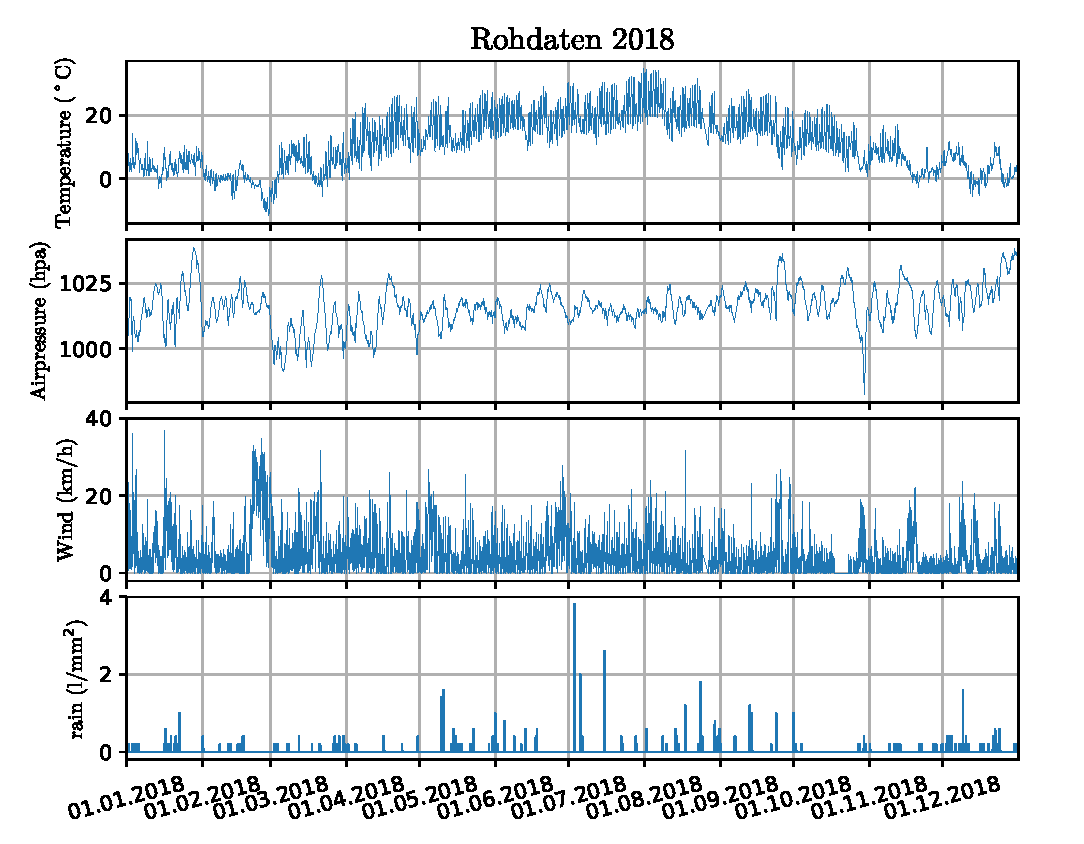
\includegraphics[width=1\textwidth]{papers/wwt/images/raw.pdf}
	\caption{Rohdaten 2018}
	\label{fig:rawdata}
\end{figure}


\section{Stetige Wavelet-Transformation}
\rhead{Stetige Wavelet-Transformation}
Die theoretischen Grundlagen rund um die stetige Wavelet-Transformation wurden im Kapitel \ref{chapter:cwt} genaustens erläutert. 
In diesem Abschnitt der Seminararbeit wird öfters auf die Theorie des angesprochenen Kapitels \ref{chapter:cwt} referenziert ohne diese genauer zu erläutern. 

Für eine m"oglichst aussagekräftige Untersuchung der Signale, in welcher so viele Informationen gewonnen werden sollten wie m"oglich, eignet sich die stetige Wavelet-Transformation (folgend noch kurz \textit{cwt} aus dem Englischen "continuous wavelet transform"). 
Regelmässig auftretende Frequenzen können dank der \textit{cwt} gefunden und zusätzlich einem Zeitraum zugeordnet werden.
\subsection{Das verwendete Wavelet}
In
\begin{equation}
\mathcal{W}f (a,b)
=
\langle f,\psi_{a,b}\rangle
=
\frac{1}{\sqrt{|a|}}\int_{-\infty}^\infty f(t)\,\overline{
	\psi\biggl(\frac{t-b}{a}\biggr)}\,dt
\label{eq:cwt1}
\end{equation}
erkennt man die grundlegende Formel der \textit{cwt}.
Wobei das $\psi_{a,b}$ für das Mutter-Wavelet steht, welches mit dem Koeffizienten $a$ skaliert und mit $b$ verschoben wird.

Als Mutter-Wavelet wurde 
\begin{equation}
\psi_{Gabor}(t) =  c_{\sigma} e^{-\frac{1}{2}t^2} \biggl(e^{i \sigma t}- e^{-\frac{1}{2} \sigma^2} \biggr)
\label{eq:morlet}
\end{equation} \cite{online:Morlet}
verwendet, welches auch als das analytische Gabor-Wavelet bekannt ist.
Dabei gibt $\sigma$ an, wie hoch die Frequenz ist und dementsprechend auch, wie viele lokale Maxima und Minima innerhalb des Gauss'schen Fensters das Mutter-Wavelet existieren.
Weiter ist $c_{\sigma}$ eine reelle Konstante und dient zur Erf"ullung der Zulässigkeitsbedingungen in der Definition \ref{cwt:zulaessig}.
Das Morlet-Wavelet wird in der Abbildung \ref{fig:gabor_plot} \space dargestellt und $\sigma$ wurde auf 5 gesetzt.

\begin{figure}
\centering
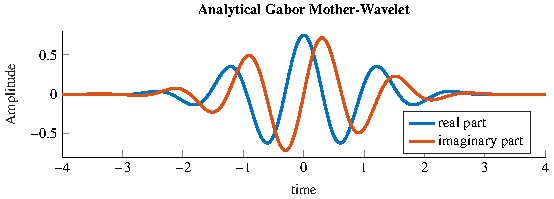
\includegraphics[width=1\textwidth]{papers/wwt/images/gabor.pdf}
\caption{Analytisches Gabor Mutter-Wavelet}
\label{fig:gabor_plot}
\end{figure}

Weiter ist zu erwähnen, dass das eben gezeigte Gabor Wavelet der referenzierten Quelle entnommen wurde. Ob Matlab die selbe Form verwendet, konnte nicht abschliessend geklärt werden.

\subsection{Berechung mit Matlab}
Die Berechnung der \textit{cwt} wurde mit der numerischen Berechnungs-Software Matlab durchgeführt.
Die dafür verwendete Funktion war die cwt()-Funktion.
Die Funktion arbeitete bei korrekter Parametrisierung wie gewünscht.
Falls man verstehen möchte wie die Funktion genau rechnet, muss man sich mit einer eher dürftigen Dokumentation herumschlagen.
Folgende Parameter wurden verwendet
\lstinputlisting[language=Matlab,firstline=1,lastline=1,  numbers=left, style = mystyle]{papers/wwt/code/matlab.m}
\label{fig:matlab_code_cwt}
wobei Matlab das Gabor-Wavelet als \texttt{'amor'} bezeichnet, mit \texttt{'VoicesPerOctave'} konnte die Genauigkeit erhöht werden und die Variable \texttt{'fs'} beschreibt die Abtastfrequenz der Messsignale.
Bei den Rückgabewerten werden die Wavelet-Werte in \texttt{'wt'} als komplexe Matrix und die approximierten Frequenzen in \texttt{'F'} abgespeichert.

Anstelle des Skalierungsfaktors $a$ in der Gleichung \ref{eq:cwt} berechnet Matlab eine approximierte Frequenz und gibt diese zurück.
Für jeden verwendeten Skalierungsfaktor $a$ wird eine Sinuskurve gesucht, die am ehesten mit der Frequenz des entsprechenden Wavelets übereinstimmt.
Siehe das Beispiel mit einem Daubechies Wavelet der Nummer 7 in der Abbildung \ref{fig:centerf}.
Dies dient dazu den Wavelet-Koeffizienten einer Frequenz zuzuordnen. 
Aus dem verwendeten Skalierungsfaktor $a$ könnte auf die Schnelle keine Information entnommen werden.
\begin{figure}[h]
	\centering
	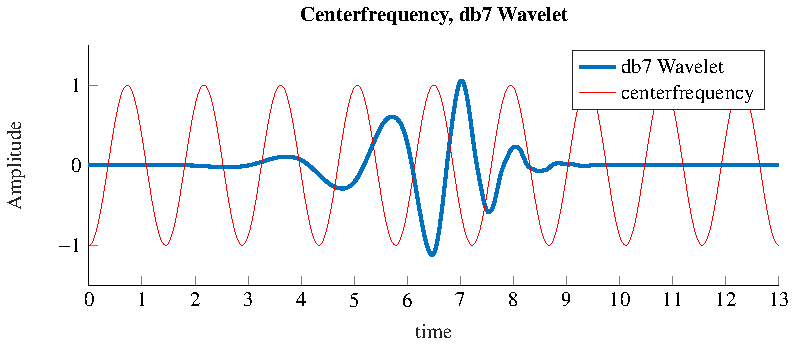
\includegraphics[width=1\textwidth]{papers/wwt/images/centerf.pdf}
	\caption{Approximierte Frequenz eines db7-Wavelet}
	\label{fig:centerf}
\end{figure}

\subsection{Verifikation der approximierten Frequenz}
\label{Freq}
Diese approximierte Frequenz konnte man mit den geeigneten Daten aus der aktuellen Anwendung der Wetterdaten sehr gut verifizieren.
Der Temperaturverlauf während einer Hochdruckphase ist sehr regelmässig und man sollte den 24 Stunden Tagesverlauf exakt erkennen.

Dank der Regelm"assigkeit des Temperaturverlaufs sieht man im \textit{cwt}-Plot eine Erh"ohung des Wertes bei einer gewissen Frequenz.
Die ausgelesene Frequenz beträgt $f = 1.16\cdot10^{-5} \,\text{Hz}$, die umgerechnet einer Periodendauer von $T = 86206.897\,\text{s}\approx 23\,\text{h }56\,\text{min } 47\,\text{s}$ entspricht.
Damit kann die Frequenz im Rückgabewert der Matlab-Funktion als sehr genau bezeichnet werden.
Dabei kommt weiter dazu, dass nur alle f"unf Minuten ein Datenpunkt aufgenommen wurde und somit die Abweichung zu 24 Stunden kleiner ist als die eigentliche Auflösung.

\begin{figure}[h]
	\centering
	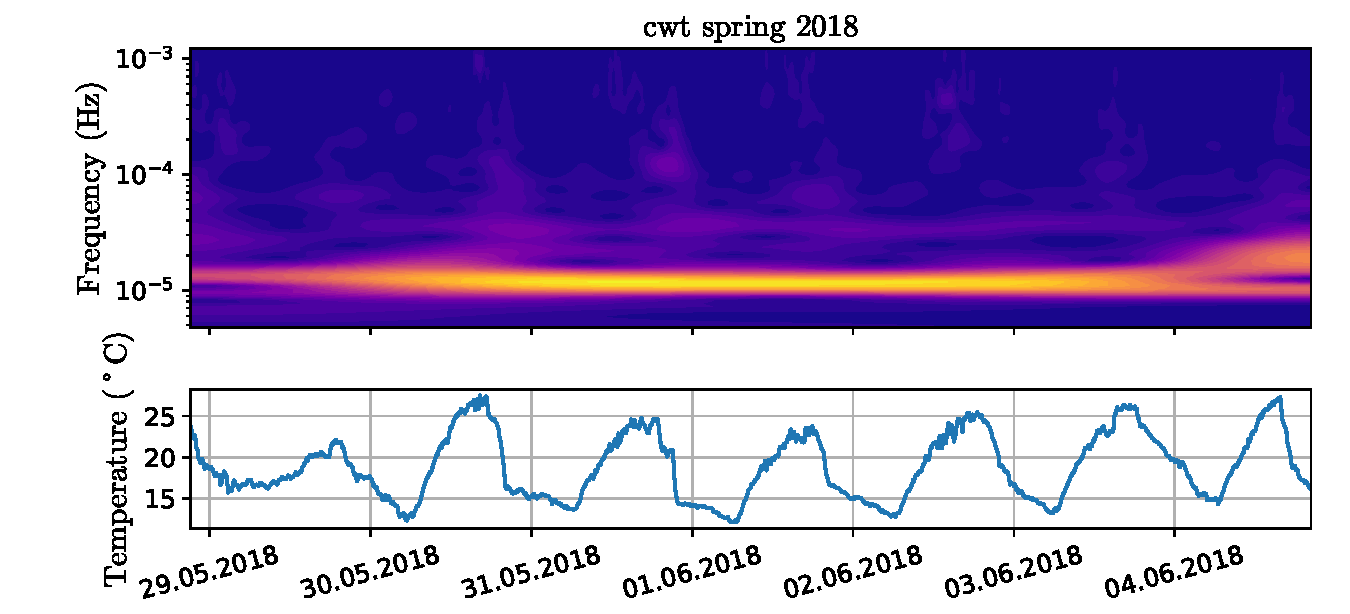
\includegraphics[width=1\textwidth]{papers/wwt/images/data_spring.pdf}
	\caption{Temperaturverlauf und entsprechende cwt}
	\label{fig:cwt_zoom}
\end{figure}



\section{Analyse von Wettereignissen}
\rhead{Analyse von Wetterereignissen}
Aufgrund der Kenntnisse rund um die \textit{cwt} kann angenommen werden, dass ein Wechsel in der Frequenz gut detektiert werden kann.
Bei einer typischen Sturmfront, welche öfters als Wintersturm in den Monaten Dezember und Januar auftreten, zeigten sich bei der Konsultation der Wetterdaten rapide Temperatur- und Luftdruckwechsel sowie ein erhöhtes Windaufkommen.
Das Ziel der Analyse war, solche Ereignisse mittels einer geeigneten \textit{cwt} zu detektieren.
Bei den Rohdaten der Frontdurchgängen erkennt man gemeinsame Wechsel im Wind, der Temperatur sowie dem Luftdruck, daher kann in der Wavelet-Transformation eine erkennbare Antwort erwartet werden. 
Diese korrelierenden auftretenden Frequenzen sollten in der \textit{cwt} sichtbar sein.

\subsection{Parallelen zur Kovarianz}

Um das korrelierende Auftreten der einzelnen Datenkanäle zu verdeutlichen, wurden bei diesen jeweils die zwei zusammengehörenden Koeffizienten der \textit{cwt} miteinander multipliziert. 
Dabei werden die Stellen hervorgehoben, wo beispielsweise der Luftdruck und die Windgeschwindigkeit abhängig voneinander variieren.  
Dies funktioniert besonders gut, da die Werte rasch gegen null gehen falls nur schon einer der beiden Datenverläufe nicht mit dem aktuellen Mutter-Wavelet übereinstimmt.
Genauer betrachtet zeigt dieses Verfahren Ähnlichkeiten mit der Formel
\begin{equation}
COV(X,Y) = \frac{\sum_{i=1}^{N} (x_i- \bar{x})(y_i- \bar{y})}{N-1},
\label{eq:kovarianz}
\end{equation}
der Kovarianz aus der Statistik. Bei dieser Anwendung wird einfach nicht die ganze Zufallsvariable benutzt, sondern nur jeweils die beiden zeitlich übereinstimmenden Werte.

Die Kovarianz zeigt sich nicht nur in dieser Anwendung. Auch schon bei der grundlegenden Formel \ref{eq:cwt1} der \textit{cwt}, kann man gewisse Parallelen sehen. 
In \ref{eq:cwt1} ist die Motivation, die jeweiligen Parameter $a$ und $b$ zu finden, wobei das Mutter-Wavelet und das Signal gemeinsam variieren.
Auch hierfür werden die Produkte der Signale berechnet, auf integriert und gemittelt.
Auch dies ist eine etwas abgewandelte Art der Kovarianz zwischen dem Datensignal und dem Mutter-Wavelet.


Die im Paper angewendete Wavelet-Transformation mit der Idee des Produktes der beiden Datenkanäle,
\begin{equation}
\begin{split}
\mathcal{W}f (a,b)
& =
\biggl<\langle Luftdruck,\psi_{a,b}\rangle, \langle Wind,\psi_{a,b} \rangle \biggr > \\
& = \biggl< \frac{1}{\sqrt{|a|}}\int_{-\infty}^\infty Luftdruck(t)\,\overline{
	\psi\biggl(\frac{t-b}{a}\biggr)}\,dt
,
\frac{1}{\sqrt{|a|}}\int_{-\infty}^\infty Wind(t)\,\overline{
	\psi\biggl(\frac{t-b}{a}\biggr)}\,dt \biggr>
\label{eq:cwt_wwt}
\end{split}
\end{equation}
kann, vorerst nur für den Luftdruck, auf die Kovarianz (Formel \ref{eq:kovarianz}) umgeschrieben werden,

\begin{equation}
COV(Luftdruck, \psi_{a,b})f(a,b) = \frac{\sum_{i=1}^{N} (Luftdruck_i - \overline{Luftdruck})(\psi_{a,b}-  \overline{\psi_{a,b}})}{N-1}.
\end{equation}
Gemäss den Zulässigkeitsbedingungen eines Mutter-Wavelets ist $\overline{\psi_{a,b}} = 0$ (Definition \ref{cwt:zulaessig}). Weiter werden Multiplikationen in Skalarprodukte umgewandelt, somit folgt;
\begin{equation}
COV(Luftdruck, \psi_{a,b})f(a,b) =  \frac{\sum_{i=1}^{N} 
 \langle Luftdruck_i- \overline{Luftdruck},\psi_{a,b}\rangle}{N-1}.
\end{equation}
Weiter Ausmultipliziert
\begin{equation}
COV(Luftdruck, \psi_{a,b})f(a,b) = \frac{\sum_{i=1}^{N} 
\langle Luftdruck_i,\psi_{a,b}\rangle - \langle \overline{Luftdruck},\psi_{a,b}\rangle}{N-1},
\end{equation}
schlussendlich ergibt sich mit $\langle \overline{Luftdruck},\psi_{a,b} \rangle = 0$,
\begin{equation}
COV(Luftdruck, \psi_{a,b})f(a,b) = \frac{\sum_{i=1}^{N} 
	\langle Luftdruck_i,\psi_{a,b}\rangle}{N-1}.
\end{equation}
 Wird noch das Produkt mit dem Wind hinzugenommen
 \begin{equation}
 \begin{split}
\biggl< COV(Luftdruck, \psi_{a,b})f(a,b), COV(Wind), \psi_{a,b})f(a,b) \biggr > \\
=
 \biggl< \frac{\sum_{i=1}^{N} 
 	\langle Luftdruck_i,\psi_{a,b}\rangle}{N-1},\frac{\sum_{i=1}^{N} 
 	\langle Wind_i,\psi_{a,b}\rangle}{N-1} \biggr >,
 \label{eq:cov_wwt}
 \end{split}
 \end{equation}
 wurde die Herleitung von der Wavelet-Transformation in der Formel \ref{eq:cwt_wwt} zum einem äquivalenten Resultat, ohne die Korrekturfaktoren, mit der Kovarianz in der Formel \ref{eq:cov_wwt} gezeigt.



\subsection{Sturmsaison 2018}
\rhead{Sturmsaison 2018}
Bereits bekannt war, dass in der Sturmsaison im Jahre 2018 einige heftige Winterstürme aufgetreten sind.
So wurde bei der Analyse der Daten nur auf diese Periode das Augenmerk gelegt. 
In Abbildung \ref{fig:cwt_storm} \space sieht man die Wavelet-Transformation des Luftdruckes und Windes miteinander multipliziert.
Dies über die Monate Januar und Februar im Jahre 2018 hinweg.
Weiter wird der Luftdruck- und Windverlauf dargestellt.
 
\begin{figure}[h]
	\centering
	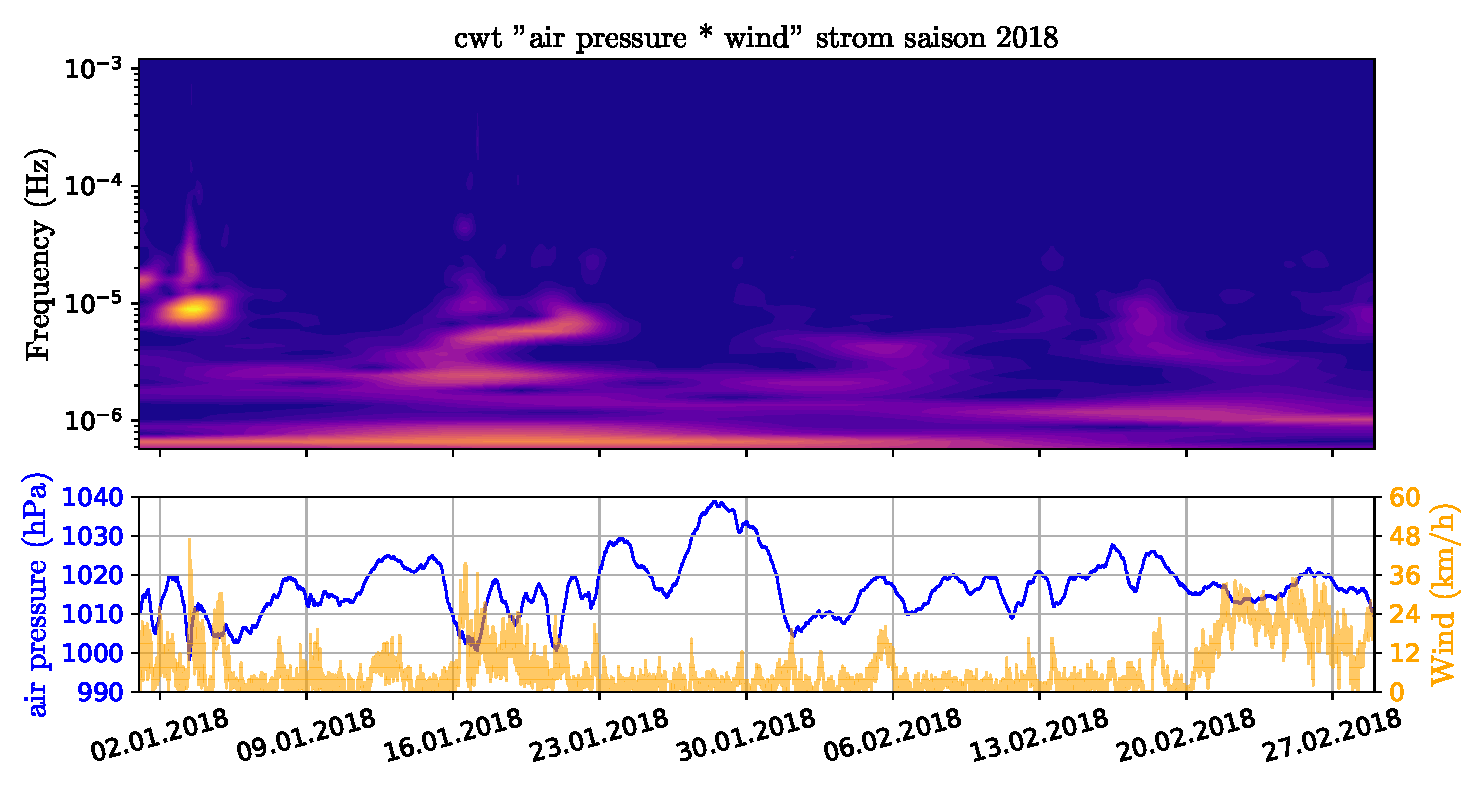
\includegraphics[width=1\textwidth]{papers/wwt/images/storm_airp_wind.pdf}
	\caption{Cwt und Rohdaten Sturmsaison 2018}
	\label{fig:cwt_storm}
\end{figure}

In Abbildung \ref{fig:cwt_storm} \space zeigen sich um den 3. sowie zwischen dem 16. und 23. Januar jeweils gewisse Frequenzen des Windes und des Luftdruckes, die gemeinsam auf die Wavelet-Transformation angesprochen haben.

\subsubsection{Wintersturm {\em Burglind} }
\label{burglind}
Hineingezoomt um den 3. Januar (Abbildung \ref{fig:cwt_storm_zoom}) sind im Rohdatenverlauf die Aktivitäten des Windes und Luftdruckes erkennbar. 
\begin{figure}[b]
	\centering
	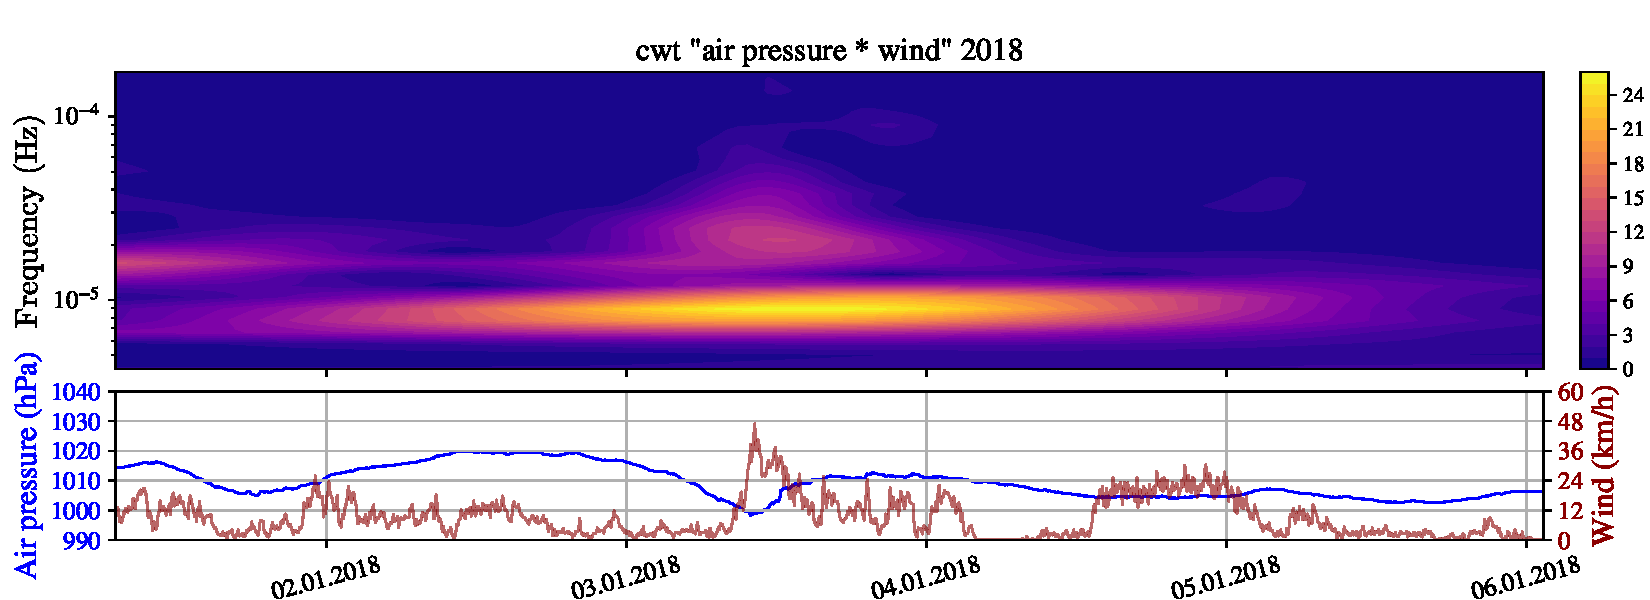
\includegraphics[width=1\textwidth]{papers/wwt/images/storm_airp_wind_zoom.pdf}
	\caption{Cwt und Rohdaten Wintersturm {\em Burglind}  2018}
	\label{fig:cwt_storm_zoom}
\end{figure}
Aus dem Fachbericht \space \cite{Fachbericht:Burglind} von Meteoschweiz war bekannt, dass am Vormittag des 3. Januars 2018 die stärkste Sturmfront seit dem verheerenden Sturm Lothar aus dem Jahre 1999 über die Schweiz zog.
Dabei zeigt sich eindrücklich, wie der Sturmdurchgang in der multiplizierten Wavelet-Transformation hervorgehoben wird.

\subsubsection{Sturmtief {\em Evi}  und {\em Friedricke} }
\label{evi}
Beim zweiten Ereignis zwischen dem 16. und 23. Januar trat die Aktivität nicht mehr so deutlich auf.
Nach dem Sturmarchiv  \cite{online:sturmarchiv} traf am 16. Januar das Sturmtief {\em Evi}  und am 18. Januar das Sturmtief {\em Friedricke} auf Europa. Dabei zeigt sich nach der Amplitude, dass das Sturmtief nicht direkt auf die Schweiz traf, sonder diese lediglich streifte. 

\begin{figure}[h]
	\centering
	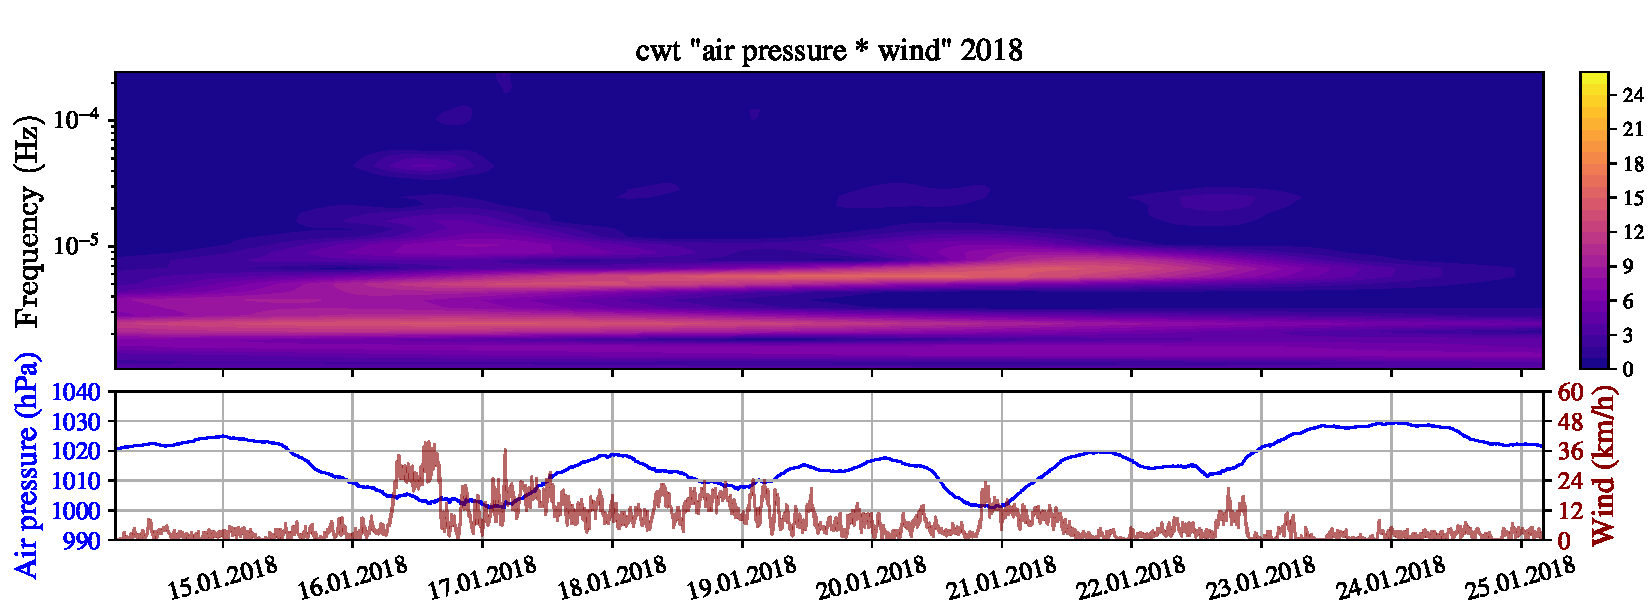
\includegraphics[width=1\textwidth]{papers/wwt/images/storm_airp_wind_zoom2.pdf}
	\caption{Cwt und Rohdaten Strumtief {\em Evi}  und {\em Friedricke} 2018}
	\label{fig:cwt_storm_zoom2}
\end{figure}



\section{Schlussfolgerung}
\rhead{Schlussfolgerung}

Mit dem Versuch, die Wavelet-Transformation im Bereich der Wetteranalyse nützlich anzuwenden, zeigt sich, dass dies durchaus möglich ist.
In der Anwendung mit dem Phänomen der Winterstürme wurde die Wavelet-Transformation oder genauer die stetige Wavelet-Transformation erfolgreich eingesetzt.
Es können zwei Hypothesen aufgestellt werden:
\begin{itemize}
	\item Die periodischen Tagesverläufe bei konstanten Wetterverhältnissen führen dazu, dass die Wavelet-Koeffizienten der \textit{cwt} bei dieser Frequenz deutlich ansteigen (\ref{Freq}).
	
	\item Nicht periodische Ereignisse äussern sich durch das korrelierte Auftreten bei der Betrachtung mehrerer Datenkanäle. Dies kann mit dem Produkt der Wavelet-Koeffizienten oder eben der Kovarianz analysiert werden (\ref{burglind}).
\end{itemize}


Damit ist selbstverständlich noch nichts abschliessend bewiesen. Die Hypothesen müssten detaillierter analysiert werden.
Auch sollte die Methode weiterführend auf andere meteorologische Ereignisse angewandt werden.
Zum Beispiel könnte man versuchen, Gewitter zu detektieren.
Falls sich diese Methode für mehrere Phänomene beweisen lässt, ist eine praktische Anwendung möglich und durchaus vorstellbar. 

\section{Anhang}
Anbei in Abbildung \ref{fig:python-plot-code} und \ref{fig:python-plot-code2} der verwendete Code zum Plotten der Abbildung \ref{fig:cwt_storm}.

\begin{figure}[h]
	\centering
	\lstinputlisting[language=Python,firstline = 1, lastline = 39, numbers=left, firstnumber=1, style = Python]{papers/wwt/code/plot_burglind.py}
	\caption{Python Codeausschnitt}
	\label{fig:python-plot-code}
\end{figure}
\begin{figure}[h]
	\centering
	\lstinputlisting[language=Python,firstline = 40, lastline = 91, firstnumber=40, numbers=left,style = Python]{papers/wwt/code/plot_burglind.py}
	\caption{Python Codeausschnitt}
	\label{fig:python-plot-code2}
\end{figure}
 
 \newpage

\printbibliography[heading=subbibliography]
\end{refsection}

%
% main.tex -- Paper zum Thema wwt
%
% (c) 2019 Michael Schmid, Hochschule Rapperswil
%
\chapter{Wetter-Wavelet-Transformation\label{chapter:wwt}}
\lhead{Wetter-Wavelet-Transformation}
\begin{refsection}
\chapterauthor{Michael Schmid}



\definecolor{codegreen}{rgb}{0,0.6,0}
\definecolor{codegray}{rgb}{0.5,0.5,0.5}
\definecolor{codepurple}{rgb}{0.58,0,0.82}
\definecolor{backcolour}{rgb}{0.95,0.95,0.92}

\lstdefinestyle{mystyle}{
	backgroundcolor=\color{backcolour},   
	commentstyle=\color{codegreen},
	keywordstyle=\color{magenta},
	numberstyle=\tiny\color{codegray},
	stringstyle=\color{codepurple},
	basicstyle=\footnotesize,
	breakatwhitespace=false,         
	breaklines=true,                 
	captionpos=b,                    
	keepspaces=true,                 
	numbers=left,                    
	numbersep=2pt,                  
	showspaces=false,                
	showstringspaces=false,
	showtabs=false,                  
	tabsize=2
}
\lstset{style=mystyle}
\lstdefinestyle{mystyle}{
	morekeywords={cwt,contourf,datetick}
}


\section{Einführung}
\rhead{Einführung}


Seit Langem konsultiere ich meine aktuellen Wetterdaten über eine eher unübliche Internetseite.
Dabei handelt es sich um eine privat geführte Wetterstation, welche die gemessenen Daten im Internet grafisch darstellt.
Die Daten werden auch tabellarisch zur Verfügung gestellt.
Das Feature, welches ich bis anhin am regelmässigsten nutzte, war die grafische Darstellung der aktuellen Wetterdaten über den Zeitraum der letzten 24 Stunden.
Bei speziellen Ereignissen im Wetterverlauf fielen mir besondere und wiederkehrende Charakteristiken auf.
\\

Nach der Einführung in die Theorie der Wavelets kam mir die Idee, solche Wetterphänomene mit einer geeigneten Wavelet Transformation zu detektieren.
In diesem Paper wird einerseits auf die theoretischen Grundlagen der angewandten Methoden zurückgegriffen sowie die besprochenen meteorologischen Phänomene kurz erläutert. 
Weiterführend wird auf die verwendeten Methoden, auch in der praktischen Anwendung, vertieft eingegangen.
Ein besonderes Augenmerk wird auf die allgemeine Vorgehensweise sowie deren Schwierigkeiten gelegt.
\\




\section{Wetterstation Seegräben}
\rhead{Wetterstation Seegräben}

Die angesprochene Wetterstation in der Gemeinde Seegräben im Kanton Zürich ist mit einer DAVIS Vantage Pro2 6153 \cite{online:davisinstruments} realisiert worden.
Sie verfügt über Sensoren für die Temperatur, Feuchtigkeit, Geschwindigkeit und Richtung des Windes sowie für den Niederschlag. 
Durch diese Sensoren werden folgende Daten aufgezeichnet:


\begin{itemize}
	\item \textbf{Aussentemperatur} in Grad Celsius
	\item \textbf{Relative Luftfeuchtigkeit} in Prozent
	\item \textbf{Luftdruck} in hPa
	\item \textbf{Windgeschwindigkeit} in km/h, gemittelt über 5 Minuten
	\item \textbf{Windböen} in km/h
	\item \textbf{Windrichtung} nach Himmelsrichtung
	\item \textbf{Regenmenge} in $\text{l/m}^{2}$
\end{itemize}	


Der Thermo- / Feuchtigkeitssensor liegt zusammen mit dem Regenmengenmesser auf 2 Meter über Boden.
Mit einem Abstand von rund 10 Meter zum nächsten Gebäude sind optimale Messbedingungen geschaffen.
Mit einem Mast ist der Windmesser auf 1.5 Meter über dem First eines Gebäudes lokalisiert \space \cite{online:wss}.
Die Daten werden anschliessend mit einer Software von PC-Wetterstation.de weiterverarbeitet und auf der Website \cite{online:wss} veröffentlicht.
Mehr zur Verwendung der Wetterdaten im n\"achsten Abschnitt.

\section{Datenaufarbeitung}
\rhead{Datenaufarbeitung}
Der n\"achste Vorbereitungsschritt zur Wavelet Transformation war die Aufbereitung der zur Verf\"ugung gestellten Daten der Wetterstation. Dazu musste erst analysiert werden, wie die Daten auf der Website dargestellt werden.
\subsection{Wetter-Archiv}
Auf der Website gibt es mehrere Möglichkeiten, sich Wetterdaten aus der Vergangenheit darstellen zu lassen.
In der Kategorie des Archivs auf der Website kann man die Wetterdaten eines gew\"unschten Zeitraums tabellarisch oder grafisch darstellen lassen.
Vom Betreiber der Website steht keine Funktion zur Verfügung, welche es erlaubt, die Daten offiziell und automatisch herunterzuladen.
\subsection{Datenerfassung}
Da f\"ur die angestrebte Anwendung eine m\"oglichst hohe Aufl\"osung der jeweiligen Daten erforderlich ist, mussten die Daten im Zeitraum von einem Tag dargestellt werden.
Dies hatte zur Folge, dass man f\"ur jeden Tag eine Tabelle auf dem Archiv der Website \"offnen musste. Man hätte anschliessend die Daten mit copy and paste in eine Excel-Tabelle einf\"ugen können. Daher wurde  entschieden, ein Programm zu schreiben, welches diese Aufgabe automatisieren sollte.
Als Programmiersprache wurde hierf\"ur Python gewählt.


Mit der Pandas Library und der Funktion \texttt{'read\_html'} \space konnten die Daten direkt aus dem Python Programm von der Website heruntergeladen werden.
Entscheidend für das Gelingen dieser Teilaufgabe war, dass die URL-Links der einzelnen Tage stets regelmässig aufgebaut sind:
\\
\\
$$\centering{\textit{https://www.wetter-seegraeben.ch/uploads/insert.php?insert=\textbf{20190701}.htm}}$$
\\
Wie zu sehen ist, wird der Link mit dem Datum regelmässig aufgebaut. Somit konnten die entsprechenden Links mit mehreren While-Schleife zusammengesetzt werden.
In der Abbildung \ref{fig:python-code} ist der wesentliche Ausschnitt aus dem Python Code dargestellt.
\begin{figure}
	\centering
	\lstinputlisting[language=Python,firstline=1,lastline=16,numbers=left,style = Python]{papers/wwt/code/get_data.py}
	\caption{Python Codeausschnitt}
	\label{fig:python-code}
\end{figure}
Die Daten konnten im nächsten Schritt in einer Excel-Tabelle abgespeichert werden.
Dort folgte der letzte Feinschliff; d.h. alle überflüssigen Kopfzeilen und Statistiken wurden entfernt.

\subsubsection{Unregelmässigkeiten der Wetterstation}
Bei der Datenerfassung durch das eben beschriebene Python Programm wurden einige Unregelmässigkeiten der Wetterstation beobachtet.
Das Programm wird jeweils durch eine Fehlermeldung abgebrochen, wenn der angegebene Link nicht abrufbar ist. 
So fiel auf, dass unregelmässig auf das Jahr verteilt, Daten von gewissen Tagen fehlten. Es stellte sich heraus, dass hinter dem eigentlich korrektem Link die entsprechende Internetseite nicht zur Verfügung steht.
Wird manuell auf der Website nach diesem Tag gesucht, kann nichts gefunden werden.
Dies trat teilweise sogar in Abschnitten von mehreren Tagen auf.
Wie sich später herausstellte, traten die fehlenden Tagen nicht zu den Zeitpunkten auf, die mich interessierten.


\subsection{Datendarstellung}
Die Darstellung der gewonnenen Daten konnte einfach mittels Python realisiert werden.
Anbei in Abbildung \ref{fig:rawdata} der Plot der Rohdaten aus dem Jahre 2018, wobei nur jeder zehnte Messpunkt verwendet wurde.
Diese Rohdaten dienten als Grundlage für alle weiteren Berechnungen. 
\begin{figure}
	\centering
	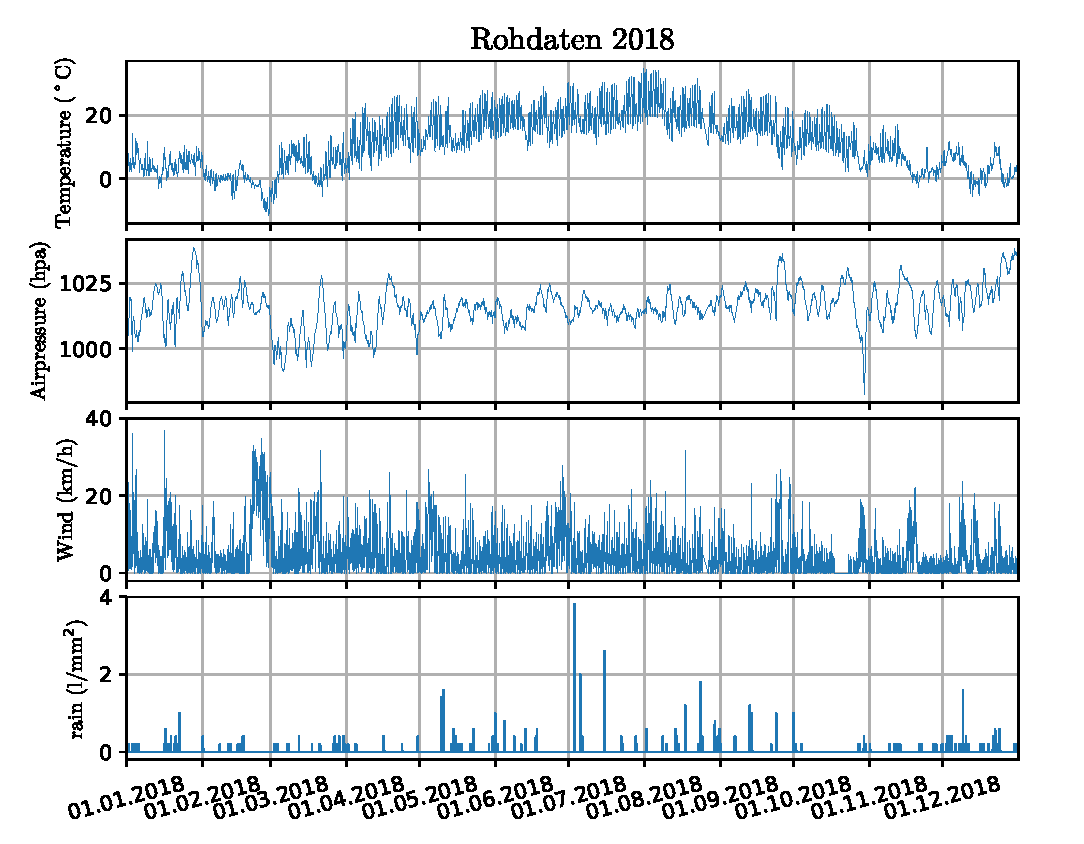
\includegraphics[width=1\textwidth]{papers/wwt/images/raw.pdf}
	\caption{Rohdaten 2018}
	\label{fig:rawdata}
\end{figure}


\section{Stetige Wavelet-Transformation}
\rhead{Stetige Wavelet-Transformation}
Die theoretischen Grundlagen rund um die stetige Wavelet-Transformation wurden im Kapitel \ref{chapter:cwt} genaustens erläutert. 
In diesem Abschnitt der Seminararbeit wird öfters auf die Theorie des angesprochenen Kapitels \ref{chapter:cwt} referenziert ohne diese genauer zu erläutern. 

Für eine m"oglichst aussagekräftige Untersuchung der Signale, in welcher so viele Informationen gewonnen werden sollten wie m"oglich, eignet sich die stetige Wavelet-Transformation (folgend noch kurz \textit{cwt} aus dem Englischen "continuous wavelet transform"). 
Regelmässig auftretende Frequenzen können dank der \textit{cwt} gefunden und zusätzlich einem Zeitraum zugeordnet werden.
\subsection{Das verwendete Wavelet}
In
\begin{equation}
\mathcal{W}f (a,b)
=
\langle f,\psi_{a,b}\rangle
=
\frac{1}{\sqrt{|a|}}\int_{-\infty}^\infty f(t)\,\overline{
	\psi\biggl(\frac{t-b}{a}\biggr)}\,dt
\label{eq:cwt1}
\end{equation}
erkennt man die grundlegende Formel der \textit{cwt}.
Wobei das $\psi_{a,b}$ für das Mutter-Wavelet steht, welches mit dem Koeffizienten $a$ skaliert und mit $b$ verschoben wird.

Als Mutter-Wavelet wurde 
\begin{equation}
\psi_{Gabor}(t) =  c_{\sigma} e^{-\frac{1}{2}t^2} \biggl(e^{i \sigma t}- e^{-\frac{1}{2} \sigma^2} \biggr)
\label{eq:morlet}
\end{equation} \cite{online:Morlet}
verwendet, welches auch als das analytische Gabor-Wavelet bekannt ist.
Dabei gibt $\sigma$ an, wie hoch die Frequenz ist und dementsprechend auch, wie viele lokale Maxima und Minima innerhalb des Gauss'schen Fensters das Mutter-Wavelet existieren.
Weiter ist $c_{\sigma}$ eine reelle Konstante und dient zur Erf"ullung der Zulässigkeitsbedingungen in der Definition \ref{cwt:zulaessig}.
Das Morlet-Wavelet wird in der Abbildung \ref{fig:gabor_plot} \space dargestellt und $\sigma$ wurde auf 5 gesetzt.

\begin{figure}
\centering
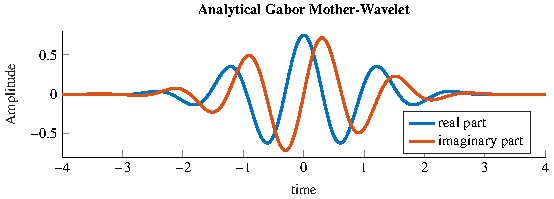
\includegraphics[width=1\textwidth]{papers/wwt/images/gabor.pdf}
\caption{Analytisches Gabor Mutter-Wavelet}
\label{fig:gabor_plot}
\end{figure}

Weiter ist zu erwähnen, dass das eben gezeigte Gabor Wavelet der referenzierten Quelle entnommen wurde. Ob Matlab die selbe Form verwendet, konnte nicht abschliessend geklärt werden.

\subsection{Berechung mit Matlab}
Die Berechnung der \textit{cwt} wurde mit der numerischen Berechnungs-Software Matlab durchgeführt.
Die dafür verwendete Funktion war die cwt()-Funktion.
Die Funktion arbeitete bei korrekter Parametrisierung wie gewünscht.
Falls man verstehen möchte wie die Funktion genau rechnet, muss man sich mit einer eher dürftigen Dokumentation herumschlagen.
Folgende Parameter wurden verwendet
\lstinputlisting[language=Matlab,firstline=1,lastline=1,  numbers=left, style = mystyle]{papers/wwt/code/matlab.m}
\label{fig:matlab_code_cwt}
wobei Matlab das Gabor-Wavelet als \texttt{'amor'} bezeichnet, mit \texttt{'VoicesPerOctave'} konnte die Genauigkeit erhöht werden und die Variable \texttt{'fs'} beschreibt die Abtastfrequenz der Messsignale.
Bei den Rückgabewerten werden die Wavelet-Werte in \texttt{'wt'} als komplexe Matrix und die approximierten Frequenzen in \texttt{'F'} abgespeichert.

Anstelle des Skalierungsfaktors $a$ in der Gleichung \ref{eq:cwt} berechnet Matlab eine approximierte Frequenz und gibt diese zurück.
Für jeden verwendeten Skalierungsfaktor $a$ wird eine Sinuskurve gesucht, die am ehesten mit der Frequenz des entsprechenden Wavelets übereinstimmt.
Siehe das Beispiel mit einem Daubechies Wavelet der Nummer 7 in der Abbildung \ref{fig:centerf}.
Dies dient dazu den Wavelet-Koeffizienten einer Frequenz zuzuordnen. 
Aus dem verwendeten Skalierungsfaktor $a$ könnte auf die Schnelle keine Information entnommen werden.
\begin{figure}[h]
	\centering
	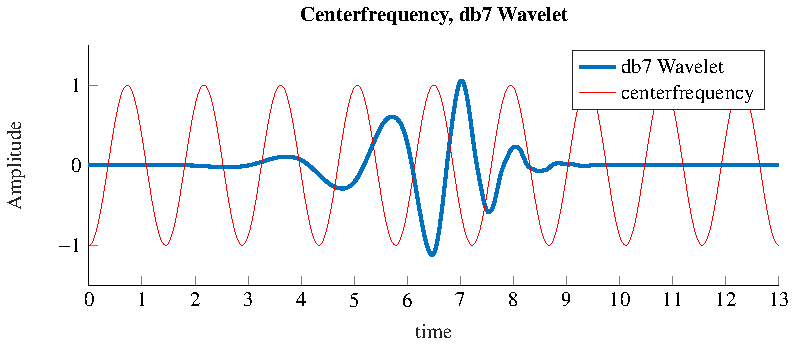
\includegraphics[width=1\textwidth]{papers/wwt/images/centerf.pdf}
	\caption{Approximierte Frequenz eines db7-Wavelet}
	\label{fig:centerf}
\end{figure}

\subsection{Verifikation der approximierten Frequenz}
\label{Freq}
Diese approximierte Frequenz konnte man mit den geeigneten Daten aus der aktuellen Anwendung der Wetterdaten sehr gut verifizieren.
Der Temperaturverlauf während einer Hochdruckphase ist sehr regelmässig und man sollte den 24 Stunden Tagesverlauf exakt erkennen.

Dank der Regelm"assigkeit des Temperaturverlaufs sieht man im \textit{cwt}-Plot eine Erh"ohung des Wertes bei einer gewissen Frequenz.
Die ausgelesene Frequenz beträgt $f = 1.16\cdot10^{-5} \,\text{Hz}$, die umgerechnet einer Periodendauer von $T = 86206.897\,\text{s}\approx 23\,\text{h }56\,\text{min } 47\,\text{s}$ entspricht.
Damit kann die Frequenz im Rückgabewert der Matlab-Funktion als sehr genau bezeichnet werden.
Dabei kommt weiter dazu, dass nur alle f"unf Minuten ein Datenpunkt aufgenommen wurde und somit die Abweichung zu 24 Stunden kleiner ist als die eigentliche Auflösung.

\begin{figure}[h]
	\centering
	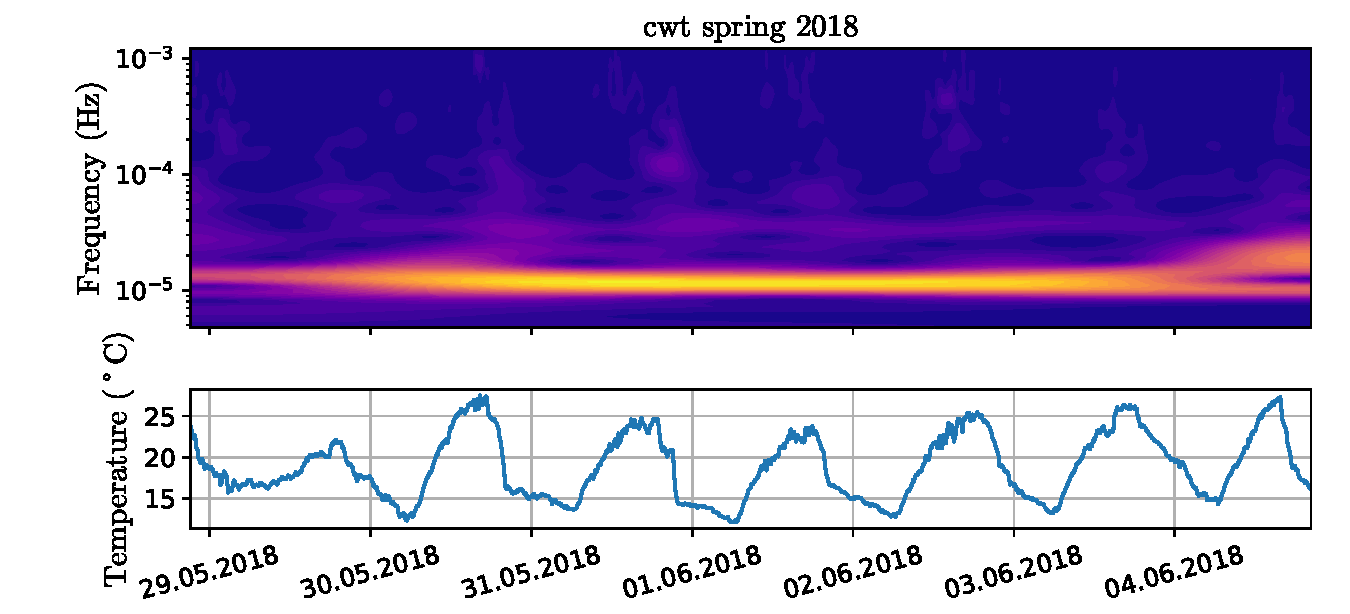
\includegraphics[width=1\textwidth]{papers/wwt/images/data_spring.pdf}
	\caption{Temperaturverlauf und entsprechende cwt}
	\label{fig:cwt_zoom}
\end{figure}



\section{Analyse von Wettereignissen}
\rhead{Analyse von Wetterereignissen}
Aufgrund der Kenntnisse rund um die \textit{cwt} kann angenommen werden, dass ein Wechsel in der Frequenz gut detektiert werden kann.
Bei einer typischen Sturmfront, welche öfters als Wintersturm in den Monaten Dezember und Januar auftreten, zeigten sich bei der Konsultation der Wetterdaten rapide Temperatur- und Luftdruckwechsel sowie ein erhöhtes Windaufkommen.
Das Ziel der Analyse war, solche Ereignisse mittels einer geeigneten \textit{cwt} zu detektieren.
Bei den Rohdaten der Frontdurchgängen erkennt man gemeinsame Wechsel im Wind, der Temperatur sowie dem Luftdruck, daher kann in der Wavelet-Transformation eine erkennbare Antwort erwartet werden. 
Diese korrelierenden auftretenden Frequenzen sollten in der \textit{cwt} sichtbar sein.

\subsection{Parallelen zur Kovarianz}

Um das korrelierende Auftreten der einzelnen Datenkanäle zu verdeutlichen, wurden bei diesen jeweils die zwei zusammengehörenden Koeffizienten der \textit{cwt} miteinander multipliziert. 
Dabei werden die Stellen hervorgehoben, wo beispielsweise der Luftdruck und die Windgeschwindigkeit abhängig voneinander variieren.  
Dies funktioniert besonders gut, da die Werte rasch gegen null gehen falls nur schon einer der beiden Datenverläufe nicht mit dem aktuellen Mutter-Wavelet übereinstimmt.
Genauer betrachtet zeigt dieses Verfahren Ähnlichkeiten mit der Formel
\begin{equation}
COV(X,Y) = \frac{\sum_{i=1}^{N} (x_i- \bar{x})(y_i- \bar{y})}{N-1},
\label{eq:kovarianz}
\end{equation}
der Kovarianz aus der Statistik. Bei dieser Anwendung wird einfach nicht die ganze Zufallsvariable benutzt, sondern nur jeweils die beiden zeitlich übereinstimmenden Werte.

Die Kovarianz zeigt sich nicht nur in dieser Anwendung. Auch schon bei der grundlegenden Formel \ref{eq:cwt1} der \textit{cwt}, kann man gewisse Parallelen sehen. 
In \ref{eq:cwt1} ist die Motivation, die jeweiligen Parameter $a$ und $b$ zu finden, wobei das Mutter-Wavelet und das Signal gemeinsam variieren.
Auch hierfür werden die Produkte der Signale berechnet, auf integriert und gemittelt.
Auch dies ist eine etwas abgewandelte Art der Kovarianz zwischen dem Datensignal und dem Mutter-Wavelet.


Die im Paper angewendete Wavelet-Transformation mit der Idee des Produktes der beiden Datenkanäle,
\begin{equation}
\begin{split}
\mathcal{W}f (a,b)
& =
\biggl<\langle Luftdruck,\psi_{a,b}\rangle, \langle Wind,\psi_{a,b} \rangle \biggr > \\
& = \biggl< \frac{1}{\sqrt{|a|}}\int_{-\infty}^\infty Luftdruck(t)\,\overline{
	\psi\biggl(\frac{t-b}{a}\biggr)}\,dt
,
\frac{1}{\sqrt{|a|}}\int_{-\infty}^\infty Wind(t)\,\overline{
	\psi\biggl(\frac{t-b}{a}\biggr)}\,dt \biggr>
\label{eq:cwt_wwt}
\end{split}
\end{equation}
kann, vorerst nur für den Luftdruck, auf die Kovarianz (Formel \ref{eq:kovarianz}) umgeschrieben werden,

\begin{equation}
COV(Luftdruck, \psi_{a,b})f(a,b) = \frac{\sum_{i=1}^{N} (Luftdruck_i - \overline{Luftdruck})(\psi_{a,b}-  \overline{\psi_{a,b}})}{N-1}.
\end{equation}
Gemäss den Zulässigkeitsbedingungen eines Mutter-Wavelets ist $\overline{\psi_{a,b}} = 0$ (Definition \ref{cwt:zulaessig}). Weiter werden Multiplikationen in Skalarprodukte umgewandelt, somit folgt;
\begin{equation}
COV(Luftdruck, \psi_{a,b})f(a,b) =  \frac{\sum_{i=1}^{N} 
 \langle Luftdruck_i- \overline{Luftdruck},\psi_{a,b}\rangle}{N-1}.
\end{equation}
Weiter Ausmultipliziert
\begin{equation}
COV(Luftdruck, \psi_{a,b})f(a,b) = \frac{\sum_{i=1}^{N} 
\langle Luftdruck_i,\psi_{a,b}\rangle - \langle \overline{Luftdruck},\psi_{a,b}\rangle}{N-1},
\end{equation}
schlussendlich ergibt sich mit $\langle \overline{Luftdruck},\psi_{a,b} \rangle = 0$,
\begin{equation}
COV(Luftdruck, \psi_{a,b})f(a,b) = \frac{\sum_{i=1}^{N} 
	\langle Luftdruck_i,\psi_{a,b}\rangle}{N-1}.
\end{equation}
 Wird noch das Produkt mit dem Wind hinzugenommen
 \begin{equation}
 \begin{split}
\biggl< COV(Luftdruck, \psi_{a,b})f(a,b), COV(Wind), \psi_{a,b})f(a,b) \biggr > \\
=
 \biggl< \frac{\sum_{i=1}^{N} 
 	\langle Luftdruck_i,\psi_{a,b}\rangle}{N-1},\frac{\sum_{i=1}^{N} 
 	\langle Wind_i,\psi_{a,b}\rangle}{N-1} \biggr >,
 \label{eq:cov_wwt}
 \end{split}
 \end{equation}
 wurde die Herleitung von der Wavelet-Transformation in der Formel \ref{eq:cwt_wwt} zum einem äquivalenten Resultat, ohne die Korrekturfaktoren, mit der Kovarianz in der Formel \ref{eq:cov_wwt} gezeigt.



\subsection{Sturmsaison 2018}
\rhead{Sturmsaison 2018}
Bereits bekannt war, dass in der Sturmsaison im Jahre 2018 einige heftige Winterstürme aufgetreten sind.
So wurde bei der Analyse der Daten nur auf diese Periode das Augenmerk gelegt. 
In Abbildung \ref{fig:cwt_storm} \space sieht man die Wavelet-Transformation des Luftdruckes und Windes miteinander multipliziert.
Dies über die Monate Januar und Februar im Jahre 2018 hinweg.
Weiter wird der Luftdruck- und Windverlauf dargestellt.
 
\begin{figure}[h]
	\centering
	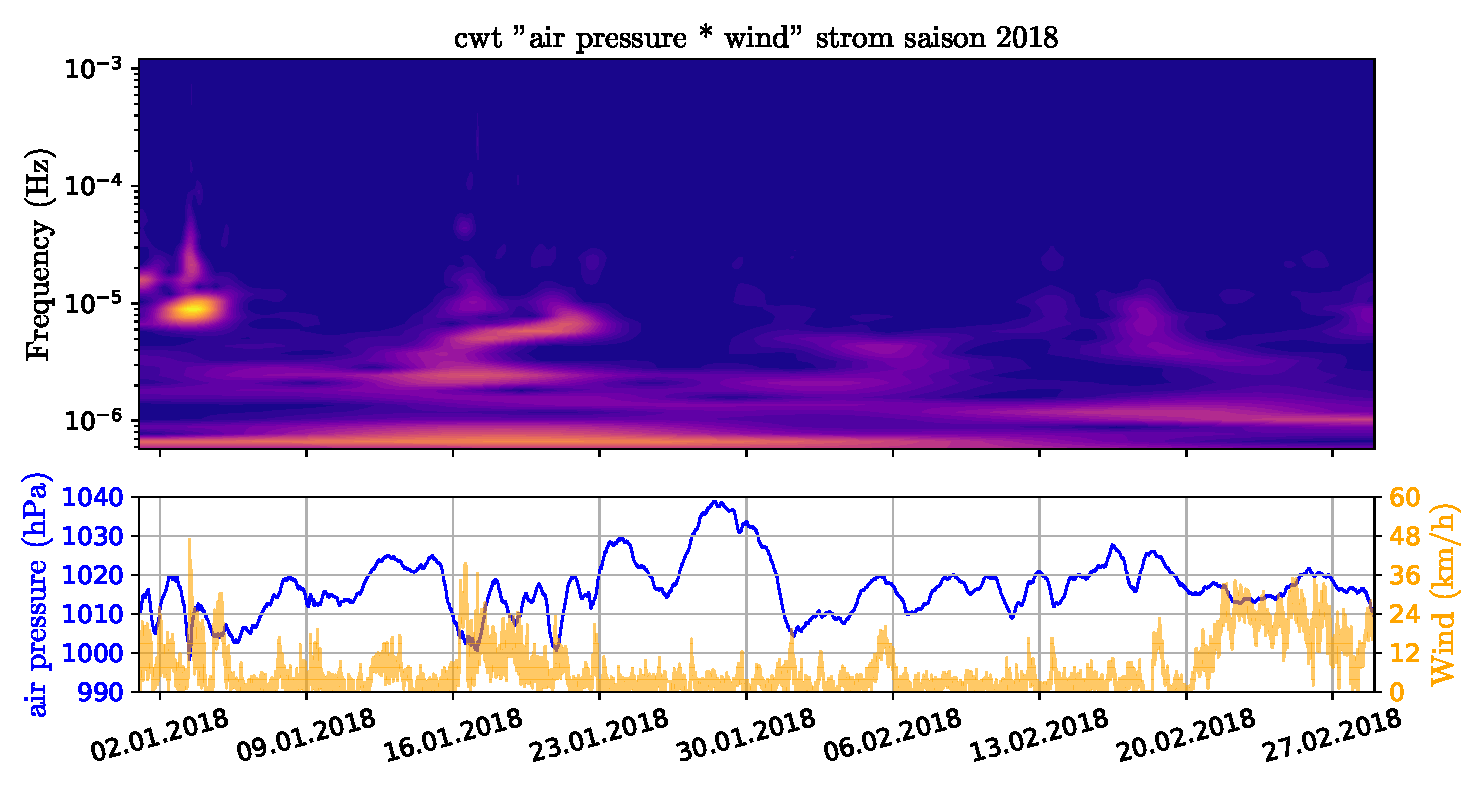
\includegraphics[width=1\textwidth]{papers/wwt/images/storm_airp_wind.pdf}
	\caption{Cwt und Rohdaten Sturmsaison 2018}
	\label{fig:cwt_storm}
\end{figure}

In Abbildung \ref{fig:cwt_storm} \space zeigen sich um den 3. sowie zwischen dem 16. und 23. Januar jeweils gewisse Frequenzen des Windes und des Luftdruckes, die gemeinsam auf die Wavelet-Transformation angesprochen haben.

\subsubsection{Wintersturm {\em Burglind} }
\label{burglind}
Hineingezoomt um den 3. Januar (Abbildung \ref{fig:cwt_storm_zoom}) sind im Rohdatenverlauf die Aktivitäten des Windes und Luftdruckes erkennbar. 
\begin{figure}[b]
	\centering
	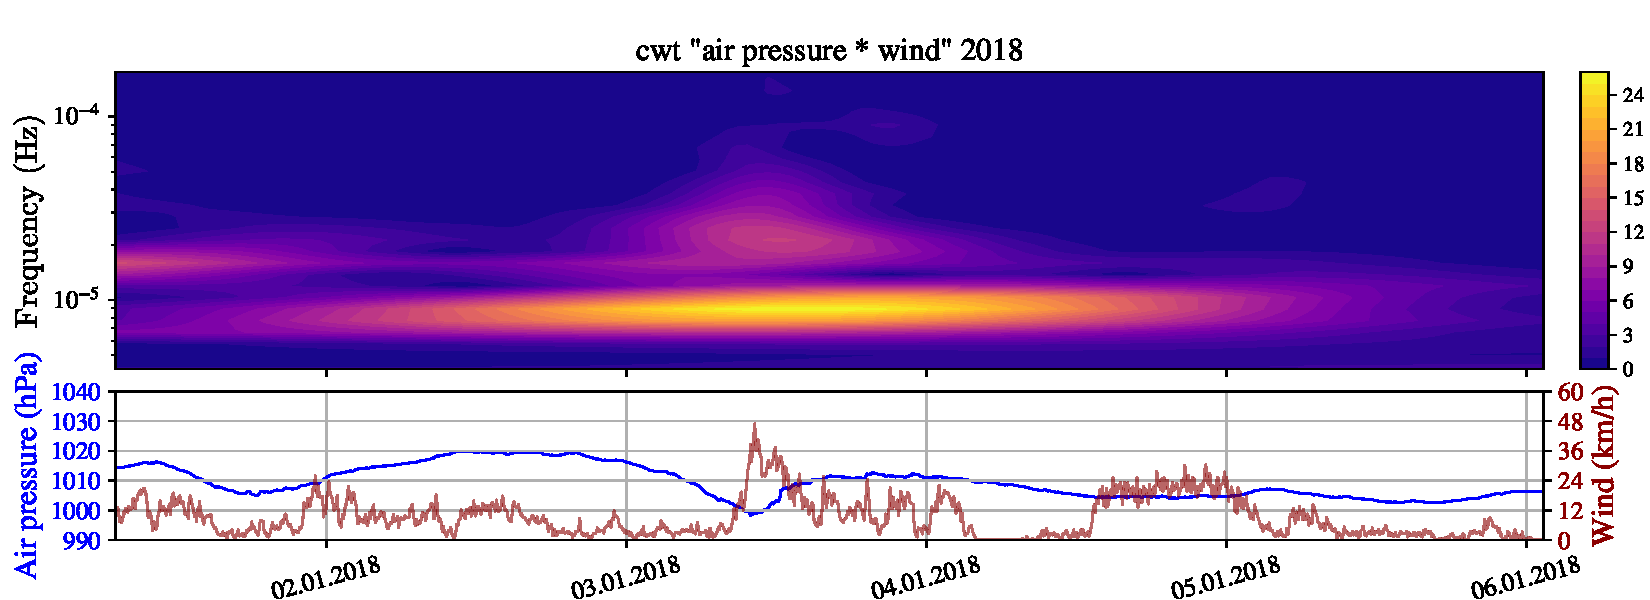
\includegraphics[width=1\textwidth]{papers/wwt/images/storm_airp_wind_zoom.pdf}
	\caption{Cwt und Rohdaten Wintersturm {\em Burglind}  2018}
	\label{fig:cwt_storm_zoom}
\end{figure}
Aus dem Fachbericht \space \cite{Fachbericht:Burglind} von Meteoschweiz war bekannt, dass am Vormittag des 3. Januars 2018 die stärkste Sturmfront seit dem verheerenden Sturm Lothar aus dem Jahre 1999 über die Schweiz zog.
Dabei zeigt sich eindrücklich, wie der Sturmdurchgang in der multiplizierten Wavelet-Transformation hervorgehoben wird.

\subsubsection{Sturmtief {\em Evi}  und {\em Friedricke} }
\label{evi}
Beim zweiten Ereignis zwischen dem 16. und 23. Januar trat die Aktivität nicht mehr so deutlich auf.
Nach dem Sturmarchiv  \cite{online:sturmarchiv} traf am 16. Januar das Sturmtief {\em Evi}  und am 18. Januar das Sturmtief {\em Friedricke} auf Europa. Dabei zeigt sich nach der Amplitude, dass das Sturmtief nicht direkt auf die Schweiz traf, sonder diese lediglich streifte. 

\begin{figure}[h]
	\centering
	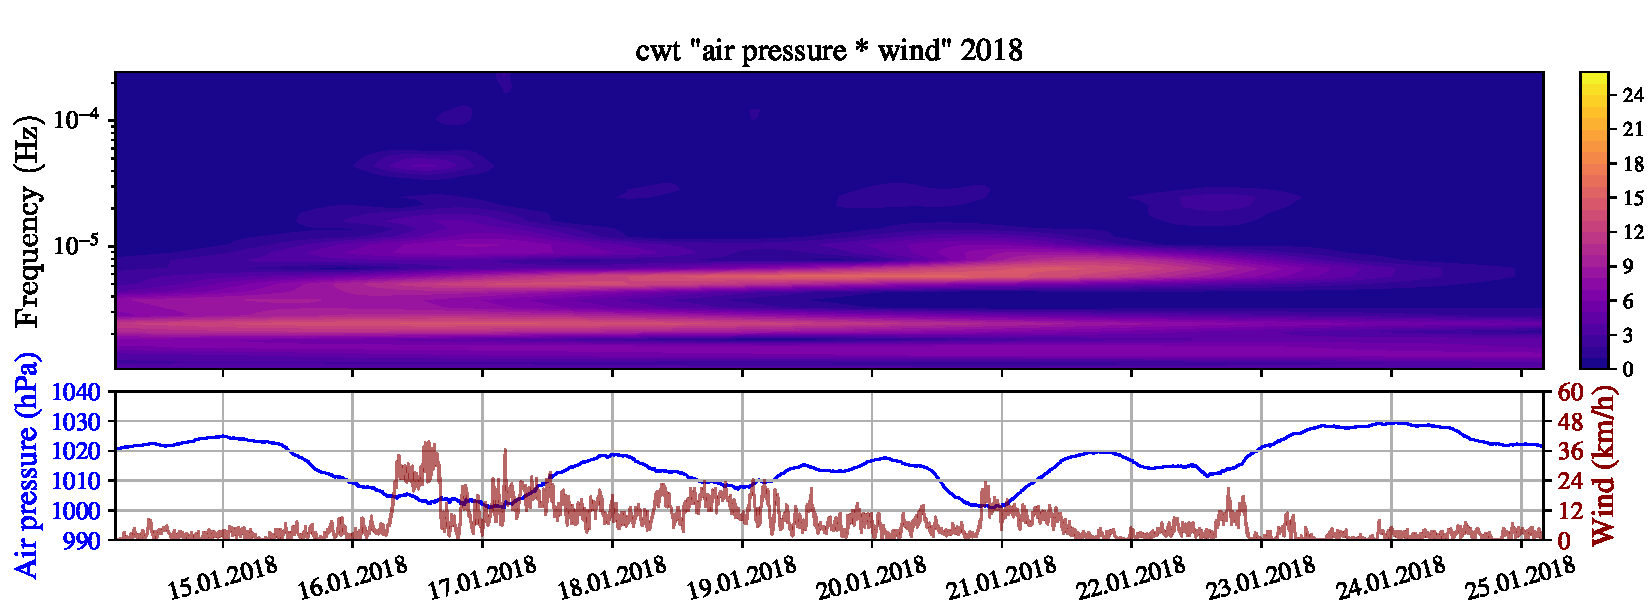
\includegraphics[width=1\textwidth]{papers/wwt/images/storm_airp_wind_zoom2.pdf}
	\caption{Cwt und Rohdaten Strumtief {\em Evi}  und {\em Friedricke} 2018}
	\label{fig:cwt_storm_zoom2}
\end{figure}



\section{Schlussfolgerung}
\rhead{Schlussfolgerung}

Mit dem Versuch, die Wavelet-Transformation im Bereich der Wetteranalyse nützlich anzuwenden, zeigt sich, dass dies durchaus möglich ist.
In der Anwendung mit dem Phänomen der Winterstürme wurde die Wavelet-Transformation oder genauer die stetige Wavelet-Transformation erfolgreich eingesetzt.
Es können zwei Hypothesen aufgestellt werden:
\begin{itemize}
	\item Die periodischen Tagesverläufe bei konstanten Wetterverhältnissen führen dazu, dass die Wavelet-Koeffizienten der \textit{cwt} bei dieser Frequenz deutlich ansteigen (\ref{Freq}).
	
	\item Nicht periodische Ereignisse äussern sich durch das korrelierte Auftreten bei der Betrachtung mehrerer Datenkanäle. Dies kann mit dem Produkt der Wavelet-Koeffizienten oder eben der Kovarianz analysiert werden (\ref{burglind}).
\end{itemize}


Damit ist selbstverständlich noch nichts abschliessend bewiesen. Die Hypothesen müssten detaillierter analysiert werden.
Auch sollte die Methode weiterführend auf andere meteorologische Ereignisse angewandt werden.
Zum Beispiel könnte man versuchen, Gewitter zu detektieren.
Falls sich diese Methode für mehrere Phänomene beweisen lässt, ist eine praktische Anwendung möglich und durchaus vorstellbar. 

\section{Anhang}
Anbei in Abbildung \ref{fig:python-plot-code} und \ref{fig:python-plot-code2} der verwendete Code zum Plotten der Abbildung \ref{fig:cwt_storm}.

\begin{figure}[h]
	\centering
	\lstinputlisting[language=Python,firstline = 1, lastline = 39, numbers=left, firstnumber=1, style = Python]{papers/wwt/code/plot_burglind.py}
	\caption{Python Codeausschnitt}
	\label{fig:python-plot-code}
\end{figure}
\begin{figure}[h]
	\centering
	\lstinputlisting[language=Python,firstline = 40, lastline = 91, firstnumber=40, numbers=left,style = Python]{papers/wwt/code/plot_burglind.py}
	\caption{Python Codeausschnitt}
	\label{fig:python-plot-code2}
\end{figure}
 
 \newpage

\printbibliography[heading=subbibliography]
\end{refsection}

%
% main.tex -- Paper zum Thema wwt
%
% (c) 2019 Michael Schmid, Hochschule Rapperswil
%
\chapter{Wetter-Wavelet-Transformation\label{chapter:wwt}}
\lhead{Wetter-Wavelet-Transformation}
\begin{refsection}
\chapterauthor{Michael Schmid}



\definecolor{codegreen}{rgb}{0,0.6,0}
\definecolor{codegray}{rgb}{0.5,0.5,0.5}
\definecolor{codepurple}{rgb}{0.58,0,0.82}
\definecolor{backcolour}{rgb}{0.95,0.95,0.92}

\lstdefinestyle{mystyle}{
	backgroundcolor=\color{backcolour},   
	commentstyle=\color{codegreen},
	keywordstyle=\color{magenta},
	numberstyle=\tiny\color{codegray},
	stringstyle=\color{codepurple},
	basicstyle=\footnotesize,
	breakatwhitespace=false,         
	breaklines=true,                 
	captionpos=b,                    
	keepspaces=true,                 
	numbers=left,                    
	numbersep=2pt,                  
	showspaces=false,                
	showstringspaces=false,
	showtabs=false,                  
	tabsize=2
}
\lstset{style=mystyle}
\lstdefinestyle{mystyle}{
	morekeywords={cwt,contourf,datetick}
}


\section{Einführung}
\rhead{Einführung}


Seit Langem konsultiere ich meine aktuellen Wetterdaten über eine eher unübliche Internetseite.
Dabei handelt es sich um eine privat geführte Wetterstation, welche die gemessenen Daten im Internet grafisch darstellt.
Die Daten werden auch tabellarisch zur Verfügung gestellt.
Das Feature, welches ich bis anhin am regelmässigsten nutzte, war die grafische Darstellung der aktuellen Wetterdaten über den Zeitraum der letzten 24 Stunden.
Bei speziellen Ereignissen im Wetterverlauf fielen mir besondere und wiederkehrende Charakteristiken auf.
\\

Nach der Einführung in die Theorie der Wavelets kam mir die Idee, solche Wetterphänomene mit einer geeigneten Wavelet Transformation zu detektieren.
In diesem Paper wird einerseits auf die theoretischen Grundlagen der angewandten Methoden zurückgegriffen sowie die besprochenen meteorologischen Phänomene kurz erläutert. 
Weiterführend wird auf die verwendeten Methoden, auch in der praktischen Anwendung, vertieft eingegangen.
Ein besonderes Augenmerk wird auf die allgemeine Vorgehensweise sowie deren Schwierigkeiten gelegt.
\\




\section{Wetterstation Seegräben}
\rhead{Wetterstation Seegräben}

Die angesprochene Wetterstation in der Gemeinde Seegräben im Kanton Zürich ist mit einer DAVIS Vantage Pro2 6153 \cite{online:davisinstruments} realisiert worden.
Sie verfügt über Sensoren für die Temperatur, Feuchtigkeit, Geschwindigkeit und Richtung des Windes sowie für den Niederschlag. 
Durch diese Sensoren werden folgende Daten aufgezeichnet:


\begin{itemize}
	\item \textbf{Aussentemperatur} in Grad Celsius
	\item \textbf{Relative Luftfeuchtigkeit} in Prozent
	\item \textbf{Luftdruck} in hPa
	\item \textbf{Windgeschwindigkeit} in km/h, gemittelt über 5 Minuten
	\item \textbf{Windböen} in km/h
	\item \textbf{Windrichtung} nach Himmelsrichtung
	\item \textbf{Regenmenge} in $\text{l/m}^{2}$
\end{itemize}	


Der Thermo- / Feuchtigkeitssensor liegt zusammen mit dem Regenmengenmesser auf 2 Meter über Boden.
Mit einem Abstand von rund 10 Meter zum nächsten Gebäude sind optimale Messbedingungen geschaffen.
Mit einem Mast ist der Windmesser auf 1.5 Meter über dem First eines Gebäudes lokalisiert \space \cite{online:wss}.
Die Daten werden anschliessend mit einer Software von PC-Wetterstation.de weiterverarbeitet und auf der Website \cite{online:wss} veröffentlicht.
Mehr zur Verwendung der Wetterdaten im n\"achsten Abschnitt.

\section{Datenaufarbeitung}
\rhead{Datenaufarbeitung}
Der n\"achste Vorbereitungsschritt zur Wavelet Transformation war die Aufbereitung der zur Verf\"ugung gestellten Daten der Wetterstation. Dazu musste erst analysiert werden, wie die Daten auf der Website dargestellt werden.
\subsection{Wetter-Archiv}
Auf der Website gibt es mehrere Möglichkeiten, sich Wetterdaten aus der Vergangenheit darstellen zu lassen.
In der Kategorie des Archivs auf der Website kann man die Wetterdaten eines gew\"unschten Zeitraums tabellarisch oder grafisch darstellen lassen.
Vom Betreiber der Website steht keine Funktion zur Verfügung, welche es erlaubt, die Daten offiziell und automatisch herunterzuladen.
\subsection{Datenerfassung}
Da f\"ur die angestrebte Anwendung eine m\"oglichst hohe Aufl\"osung der jeweiligen Daten erforderlich ist, mussten die Daten im Zeitraum von einem Tag dargestellt werden.
Dies hatte zur Folge, dass man f\"ur jeden Tag eine Tabelle auf dem Archiv der Website \"offnen musste. Man hätte anschliessend die Daten mit copy and paste in eine Excel-Tabelle einf\"ugen können. Daher wurde  entschieden, ein Programm zu schreiben, welches diese Aufgabe automatisieren sollte.
Als Programmiersprache wurde hierf\"ur Python gewählt.


Mit der Pandas Library und der Funktion \texttt{'read\_html'} \space konnten die Daten direkt aus dem Python Programm von der Website heruntergeladen werden.
Entscheidend für das Gelingen dieser Teilaufgabe war, dass die URL-Links der einzelnen Tage stets regelmässig aufgebaut sind:
\\
\\
$$\centering{\textit{https://www.wetter-seegraeben.ch/uploads/insert.php?insert=\textbf{20190701}.htm}}$$
\\
Wie zu sehen ist, wird der Link mit dem Datum regelmässig aufgebaut. Somit konnten die entsprechenden Links mit mehreren While-Schleife zusammengesetzt werden.
In der Abbildung \ref{fig:python-code} ist der wesentliche Ausschnitt aus dem Python Code dargestellt.
\begin{figure}
	\centering
	\lstinputlisting[language=Python,firstline=1,lastline=16,numbers=left,style = Python]{papers/wwt/code/get_data.py}
	\caption{Python Codeausschnitt}
	\label{fig:python-code}
\end{figure}
Die Daten konnten im nächsten Schritt in einer Excel-Tabelle abgespeichert werden.
Dort folgte der letzte Feinschliff; d.h. alle überflüssigen Kopfzeilen und Statistiken wurden entfernt.

\subsubsection{Unregelmässigkeiten der Wetterstation}
Bei der Datenerfassung durch das eben beschriebene Python Programm wurden einige Unregelmässigkeiten der Wetterstation beobachtet.
Das Programm wird jeweils durch eine Fehlermeldung abgebrochen, wenn der angegebene Link nicht abrufbar ist. 
So fiel auf, dass unregelmässig auf das Jahr verteilt, Daten von gewissen Tagen fehlten. Es stellte sich heraus, dass hinter dem eigentlich korrektem Link die entsprechende Internetseite nicht zur Verfügung steht.
Wird manuell auf der Website nach diesem Tag gesucht, kann nichts gefunden werden.
Dies trat teilweise sogar in Abschnitten von mehreren Tagen auf.
Wie sich später herausstellte, traten die fehlenden Tagen nicht zu den Zeitpunkten auf, die mich interessierten.


\subsection{Datendarstellung}
Die Darstellung der gewonnenen Daten konnte einfach mittels Python realisiert werden.
Anbei in Abbildung \ref{fig:rawdata} der Plot der Rohdaten aus dem Jahre 2018, wobei nur jeder zehnte Messpunkt verwendet wurde.
Diese Rohdaten dienten als Grundlage für alle weiteren Berechnungen. 
\begin{figure}
	\centering
	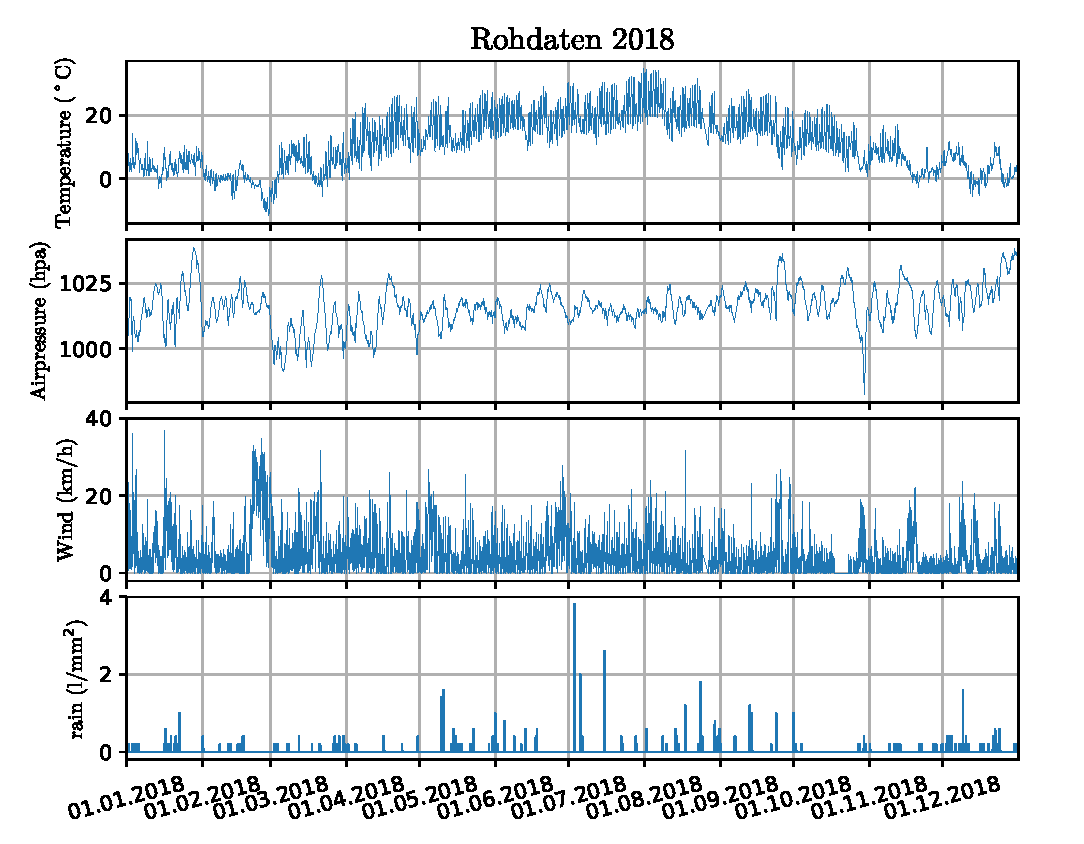
\includegraphics[width=1\textwidth]{papers/wwt/images/raw.pdf}
	\caption{Rohdaten 2018}
	\label{fig:rawdata}
\end{figure}


\section{Stetige Wavelet-Transformation}
\rhead{Stetige Wavelet-Transformation}
Die theoretischen Grundlagen rund um die stetige Wavelet-Transformation wurden im Kapitel \ref{chapter:cwt} genaustens erläutert. 
In diesem Abschnitt der Seminararbeit wird öfters auf die Theorie des angesprochenen Kapitels \ref{chapter:cwt} referenziert ohne diese genauer zu erläutern. 

Für eine m"oglichst aussagekräftige Untersuchung der Signale, in welcher so viele Informationen gewonnen werden sollten wie m"oglich, eignet sich die stetige Wavelet-Transformation (folgend noch kurz \textit{cwt} aus dem Englischen "continuous wavelet transform"). 
Regelmässig auftretende Frequenzen können dank der \textit{cwt} gefunden und zusätzlich einem Zeitraum zugeordnet werden.
\subsection{Das verwendete Wavelet}
In
\begin{equation}
\mathcal{W}f (a,b)
=
\langle f,\psi_{a,b}\rangle
=
\frac{1}{\sqrt{|a|}}\int_{-\infty}^\infty f(t)\,\overline{
	\psi\biggl(\frac{t-b}{a}\biggr)}\,dt
\label{eq:cwt1}
\end{equation}
erkennt man die grundlegende Formel der \textit{cwt}.
Wobei das $\psi_{a,b}$ für das Mutter-Wavelet steht, welches mit dem Koeffizienten $a$ skaliert und mit $b$ verschoben wird.

Als Mutter-Wavelet wurde 
\begin{equation}
\psi_{Gabor}(t) =  c_{\sigma} e^{-\frac{1}{2}t^2} \biggl(e^{i \sigma t}- e^{-\frac{1}{2} \sigma^2} \biggr)
\label{eq:morlet}
\end{equation} \cite{online:Morlet}
verwendet, welches auch als das analytische Gabor-Wavelet bekannt ist.
Dabei gibt $\sigma$ an, wie hoch die Frequenz ist und dementsprechend auch, wie viele lokale Maxima und Minima innerhalb des Gauss'schen Fensters das Mutter-Wavelet existieren.
Weiter ist $c_{\sigma}$ eine reelle Konstante und dient zur Erf"ullung der Zulässigkeitsbedingungen in der Definition \ref{cwt:zulaessig}.
Das Morlet-Wavelet wird in der Abbildung \ref{fig:gabor_plot} \space dargestellt und $\sigma$ wurde auf 5 gesetzt.

\begin{figure}
\centering
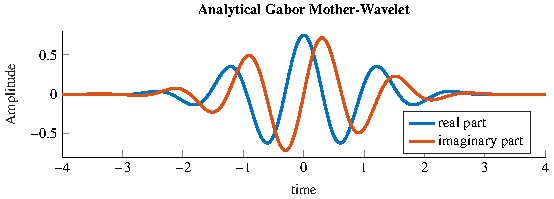
\includegraphics[width=1\textwidth]{papers/wwt/images/gabor.pdf}
\caption{Analytisches Gabor Mutter-Wavelet}
\label{fig:gabor_plot}
\end{figure}

Weiter ist zu erwähnen, dass das eben gezeigte Gabor Wavelet der referenzierten Quelle entnommen wurde. Ob Matlab die selbe Form verwendet, konnte nicht abschliessend geklärt werden.

\subsection{Berechung mit Matlab}
Die Berechnung der \textit{cwt} wurde mit der numerischen Berechnungs-Software Matlab durchgeführt.
Die dafür verwendete Funktion war die cwt()-Funktion.
Die Funktion arbeitete bei korrekter Parametrisierung wie gewünscht.
Falls man verstehen möchte wie die Funktion genau rechnet, muss man sich mit einer eher dürftigen Dokumentation herumschlagen.
Folgende Parameter wurden verwendet
\lstinputlisting[language=Matlab,firstline=1,lastline=1,  numbers=left, style = mystyle]{papers/wwt/code/matlab.m}
\label{fig:matlab_code_cwt}
wobei Matlab das Gabor-Wavelet als \texttt{'amor'} bezeichnet, mit \texttt{'VoicesPerOctave'} konnte die Genauigkeit erhöht werden und die Variable \texttt{'fs'} beschreibt die Abtastfrequenz der Messsignale.
Bei den Rückgabewerten werden die Wavelet-Werte in \texttt{'wt'} als komplexe Matrix und die approximierten Frequenzen in \texttt{'F'} abgespeichert.

Anstelle des Skalierungsfaktors $a$ in der Gleichung \ref{eq:cwt} berechnet Matlab eine approximierte Frequenz und gibt diese zurück.
Für jeden verwendeten Skalierungsfaktor $a$ wird eine Sinuskurve gesucht, die am ehesten mit der Frequenz des entsprechenden Wavelets übereinstimmt.
Siehe das Beispiel mit einem Daubechies Wavelet der Nummer 7 in der Abbildung \ref{fig:centerf}.
Dies dient dazu den Wavelet-Koeffizienten einer Frequenz zuzuordnen. 
Aus dem verwendeten Skalierungsfaktor $a$ könnte auf die Schnelle keine Information entnommen werden.
\begin{figure}[h]
	\centering
	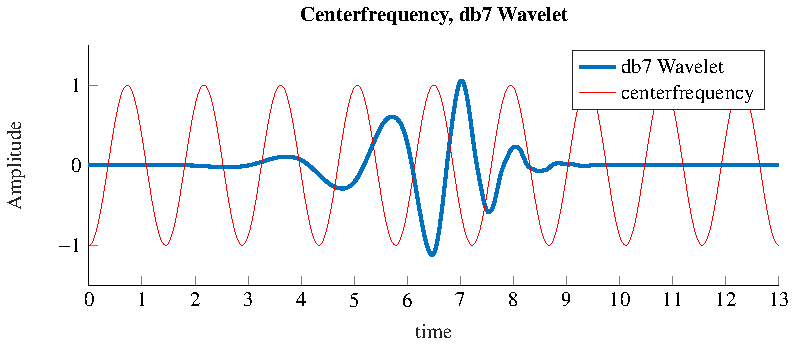
\includegraphics[width=1\textwidth]{papers/wwt/images/centerf.pdf}
	\caption{Approximierte Frequenz eines db7-Wavelet}
	\label{fig:centerf}
\end{figure}

\subsection{Verifikation der approximierten Frequenz}
\label{Freq}
Diese approximierte Frequenz konnte man mit den geeigneten Daten aus der aktuellen Anwendung der Wetterdaten sehr gut verifizieren.
Der Temperaturverlauf während einer Hochdruckphase ist sehr regelmässig und man sollte den 24 Stunden Tagesverlauf exakt erkennen.

Dank der Regelm"assigkeit des Temperaturverlaufs sieht man im \textit{cwt}-Plot eine Erh"ohung des Wertes bei einer gewissen Frequenz.
Die ausgelesene Frequenz beträgt $f = 1.16\cdot10^{-5} \,\text{Hz}$, die umgerechnet einer Periodendauer von $T = 86206.897\,\text{s}\approx 23\,\text{h }56\,\text{min } 47\,\text{s}$ entspricht.
Damit kann die Frequenz im Rückgabewert der Matlab-Funktion als sehr genau bezeichnet werden.
Dabei kommt weiter dazu, dass nur alle f"unf Minuten ein Datenpunkt aufgenommen wurde und somit die Abweichung zu 24 Stunden kleiner ist als die eigentliche Auflösung.

\begin{figure}[h]
	\centering
	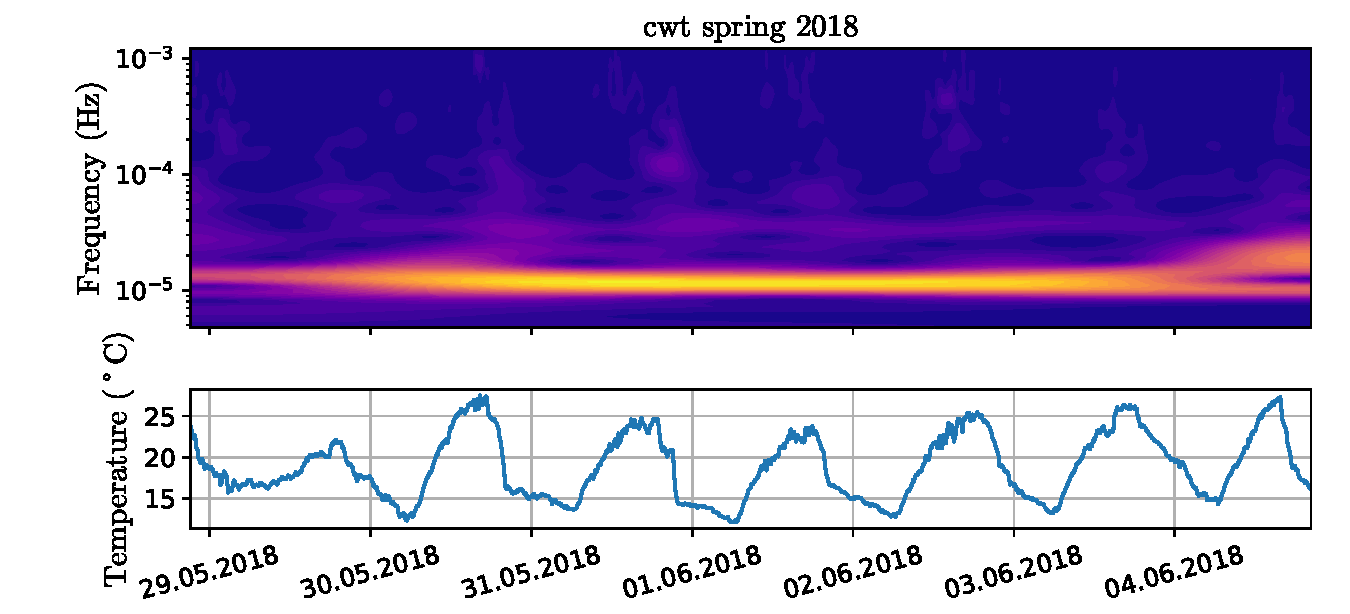
\includegraphics[width=1\textwidth]{papers/wwt/images/data_spring.pdf}
	\caption{Temperaturverlauf und entsprechende cwt}
	\label{fig:cwt_zoom}
\end{figure}



\section{Analyse von Wettereignissen}
\rhead{Analyse von Wetterereignissen}
Aufgrund der Kenntnisse rund um die \textit{cwt} kann angenommen werden, dass ein Wechsel in der Frequenz gut detektiert werden kann.
Bei einer typischen Sturmfront, welche öfters als Wintersturm in den Monaten Dezember und Januar auftreten, zeigten sich bei der Konsultation der Wetterdaten rapide Temperatur- und Luftdruckwechsel sowie ein erhöhtes Windaufkommen.
Das Ziel der Analyse war, solche Ereignisse mittels einer geeigneten \textit{cwt} zu detektieren.
Bei den Rohdaten der Frontdurchgängen erkennt man gemeinsame Wechsel im Wind, der Temperatur sowie dem Luftdruck, daher kann in der Wavelet-Transformation eine erkennbare Antwort erwartet werden. 
Diese korrelierenden auftretenden Frequenzen sollten in der \textit{cwt} sichtbar sein.

\subsection{Parallelen zur Kovarianz}

Um das korrelierende Auftreten der einzelnen Datenkanäle zu verdeutlichen, wurden bei diesen jeweils die zwei zusammengehörenden Koeffizienten der \textit{cwt} miteinander multipliziert. 
Dabei werden die Stellen hervorgehoben, wo beispielsweise der Luftdruck und die Windgeschwindigkeit abhängig voneinander variieren.  
Dies funktioniert besonders gut, da die Werte rasch gegen null gehen falls nur schon einer der beiden Datenverläufe nicht mit dem aktuellen Mutter-Wavelet übereinstimmt.
Genauer betrachtet zeigt dieses Verfahren Ähnlichkeiten mit der Formel
\begin{equation}
COV(X,Y) = \frac{\sum_{i=1}^{N} (x_i- \bar{x})(y_i- \bar{y})}{N-1},
\label{eq:kovarianz}
\end{equation}
der Kovarianz aus der Statistik. Bei dieser Anwendung wird einfach nicht die ganze Zufallsvariable benutzt, sondern nur jeweils die beiden zeitlich übereinstimmenden Werte.

Die Kovarianz zeigt sich nicht nur in dieser Anwendung. Auch schon bei der grundlegenden Formel \ref{eq:cwt1} der \textit{cwt}, kann man gewisse Parallelen sehen. 
In \ref{eq:cwt1} ist die Motivation, die jeweiligen Parameter $a$ und $b$ zu finden, wobei das Mutter-Wavelet und das Signal gemeinsam variieren.
Auch hierfür werden die Produkte der Signale berechnet, auf integriert und gemittelt.
Auch dies ist eine etwas abgewandelte Art der Kovarianz zwischen dem Datensignal und dem Mutter-Wavelet.


Die im Paper angewendete Wavelet-Transformation mit der Idee des Produktes der beiden Datenkanäle,
\begin{equation}
\begin{split}
\mathcal{W}f (a,b)
& =
\biggl<\langle Luftdruck,\psi_{a,b}\rangle, \langle Wind,\psi_{a,b} \rangle \biggr > \\
& = \biggl< \frac{1}{\sqrt{|a|}}\int_{-\infty}^\infty Luftdruck(t)\,\overline{
	\psi\biggl(\frac{t-b}{a}\biggr)}\,dt
,
\frac{1}{\sqrt{|a|}}\int_{-\infty}^\infty Wind(t)\,\overline{
	\psi\biggl(\frac{t-b}{a}\biggr)}\,dt \biggr>
\label{eq:cwt_wwt}
\end{split}
\end{equation}
kann, vorerst nur für den Luftdruck, auf die Kovarianz (Formel \ref{eq:kovarianz}) umgeschrieben werden,

\begin{equation}
COV(Luftdruck, \psi_{a,b})f(a,b) = \frac{\sum_{i=1}^{N} (Luftdruck_i - \overline{Luftdruck})(\psi_{a,b}-  \overline{\psi_{a,b}})}{N-1}.
\end{equation}
Gemäss den Zulässigkeitsbedingungen eines Mutter-Wavelets ist $\overline{\psi_{a,b}} = 0$ (Definition \ref{cwt:zulaessig}). Weiter werden Multiplikationen in Skalarprodukte umgewandelt, somit folgt;
\begin{equation}
COV(Luftdruck, \psi_{a,b})f(a,b) =  \frac{\sum_{i=1}^{N} 
 \langle Luftdruck_i- \overline{Luftdruck},\psi_{a,b}\rangle}{N-1}.
\end{equation}
Weiter Ausmultipliziert
\begin{equation}
COV(Luftdruck, \psi_{a,b})f(a,b) = \frac{\sum_{i=1}^{N} 
\langle Luftdruck_i,\psi_{a,b}\rangle - \langle \overline{Luftdruck},\psi_{a,b}\rangle}{N-1},
\end{equation}
schlussendlich ergibt sich mit $\langle \overline{Luftdruck},\psi_{a,b} \rangle = 0$,
\begin{equation}
COV(Luftdruck, \psi_{a,b})f(a,b) = \frac{\sum_{i=1}^{N} 
	\langle Luftdruck_i,\psi_{a,b}\rangle}{N-1}.
\end{equation}
 Wird noch das Produkt mit dem Wind hinzugenommen
 \begin{equation}
 \begin{split}
\biggl< COV(Luftdruck, \psi_{a,b})f(a,b), COV(Wind), \psi_{a,b})f(a,b) \biggr > \\
=
 \biggl< \frac{\sum_{i=1}^{N} 
 	\langle Luftdruck_i,\psi_{a,b}\rangle}{N-1},\frac{\sum_{i=1}^{N} 
 	\langle Wind_i,\psi_{a,b}\rangle}{N-1} \biggr >,
 \label{eq:cov_wwt}
 \end{split}
 \end{equation}
 wurde die Herleitung von der Wavelet-Transformation in der Formel \ref{eq:cwt_wwt} zum einem äquivalenten Resultat, ohne die Korrekturfaktoren, mit der Kovarianz in der Formel \ref{eq:cov_wwt} gezeigt.



\subsection{Sturmsaison 2018}
\rhead{Sturmsaison 2018}
Bereits bekannt war, dass in der Sturmsaison im Jahre 2018 einige heftige Winterstürme aufgetreten sind.
So wurde bei der Analyse der Daten nur auf diese Periode das Augenmerk gelegt. 
In Abbildung \ref{fig:cwt_storm} \space sieht man die Wavelet-Transformation des Luftdruckes und Windes miteinander multipliziert.
Dies über die Monate Januar und Februar im Jahre 2018 hinweg.
Weiter wird der Luftdruck- und Windverlauf dargestellt.
 
\begin{figure}[h]
	\centering
	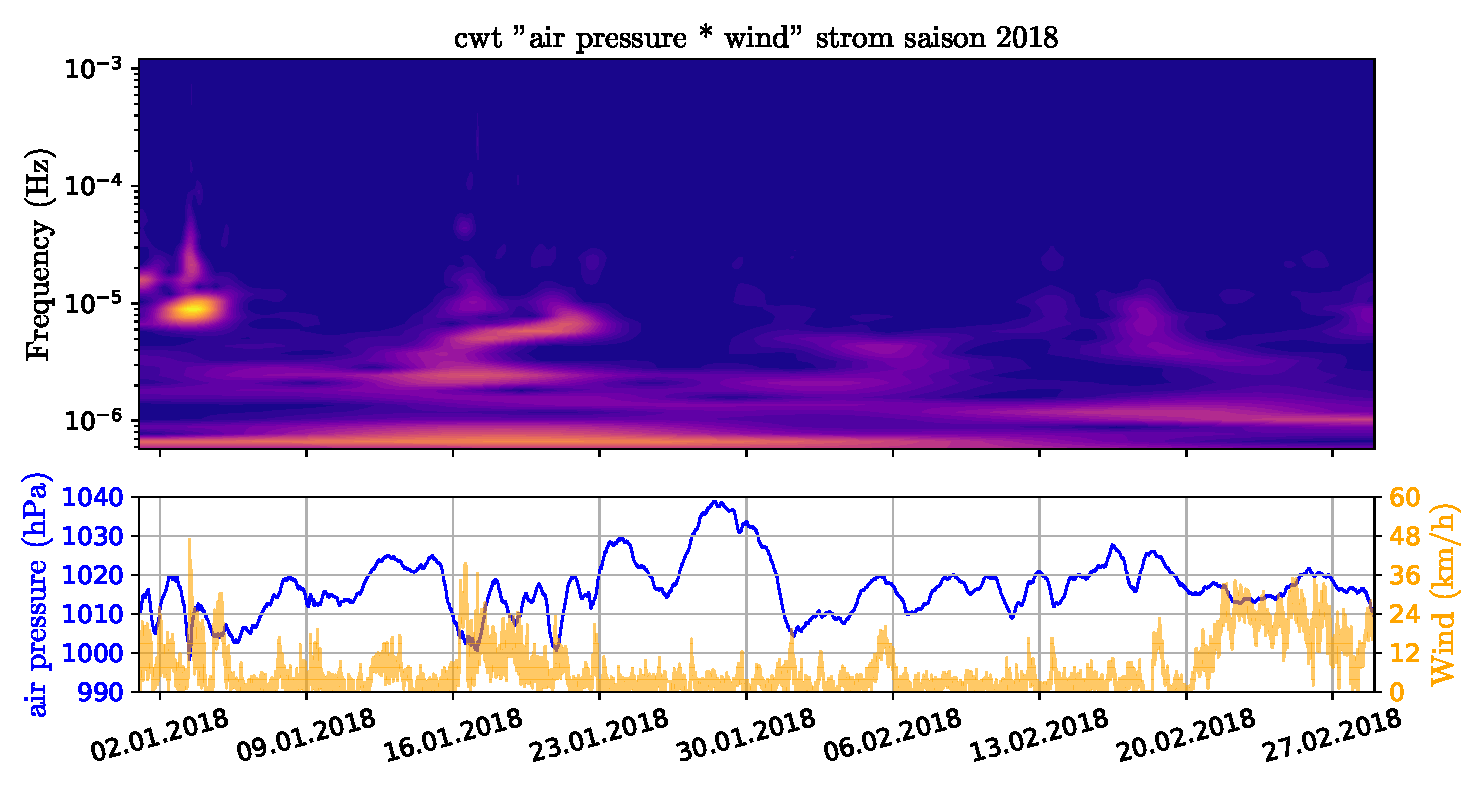
\includegraphics[width=1\textwidth]{papers/wwt/images/storm_airp_wind.pdf}
	\caption{Cwt und Rohdaten Sturmsaison 2018}
	\label{fig:cwt_storm}
\end{figure}

In Abbildung \ref{fig:cwt_storm} \space zeigen sich um den 3. sowie zwischen dem 16. und 23. Januar jeweils gewisse Frequenzen des Windes und des Luftdruckes, die gemeinsam auf die Wavelet-Transformation angesprochen haben.

\subsubsection{Wintersturm {\em Burglind} }
\label{burglind}
Hineingezoomt um den 3. Januar (Abbildung \ref{fig:cwt_storm_zoom}) sind im Rohdatenverlauf die Aktivitäten des Windes und Luftdruckes erkennbar. 
\begin{figure}[b]
	\centering
	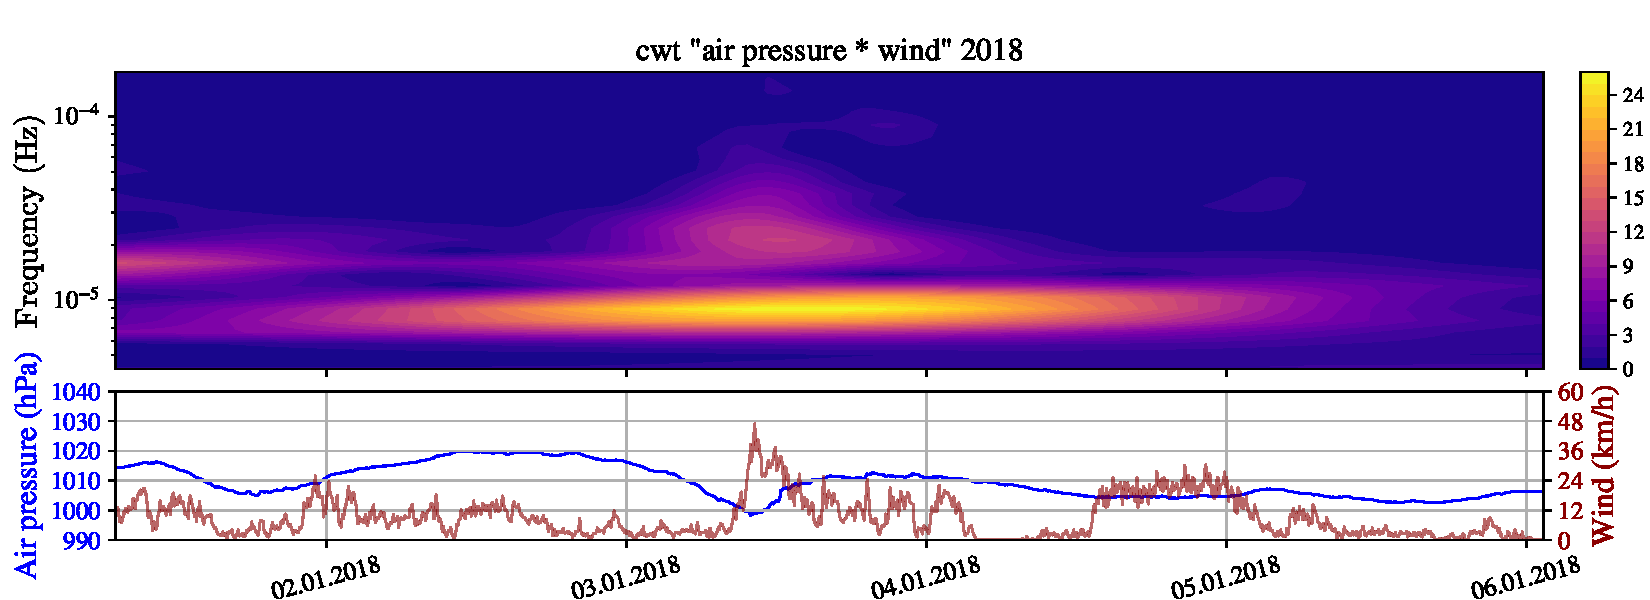
\includegraphics[width=1\textwidth]{papers/wwt/images/storm_airp_wind_zoom.pdf}
	\caption{Cwt und Rohdaten Wintersturm {\em Burglind}  2018}
	\label{fig:cwt_storm_zoom}
\end{figure}
Aus dem Fachbericht \space \cite{Fachbericht:Burglind} von Meteoschweiz war bekannt, dass am Vormittag des 3. Januars 2018 die stärkste Sturmfront seit dem verheerenden Sturm Lothar aus dem Jahre 1999 über die Schweiz zog.
Dabei zeigt sich eindrücklich, wie der Sturmdurchgang in der multiplizierten Wavelet-Transformation hervorgehoben wird.

\subsubsection{Sturmtief {\em Evi}  und {\em Friedricke} }
\label{evi}
Beim zweiten Ereignis zwischen dem 16. und 23. Januar trat die Aktivität nicht mehr so deutlich auf.
Nach dem Sturmarchiv  \cite{online:sturmarchiv} traf am 16. Januar das Sturmtief {\em Evi}  und am 18. Januar das Sturmtief {\em Friedricke} auf Europa. Dabei zeigt sich nach der Amplitude, dass das Sturmtief nicht direkt auf die Schweiz traf, sonder diese lediglich streifte. 

\begin{figure}[h]
	\centering
	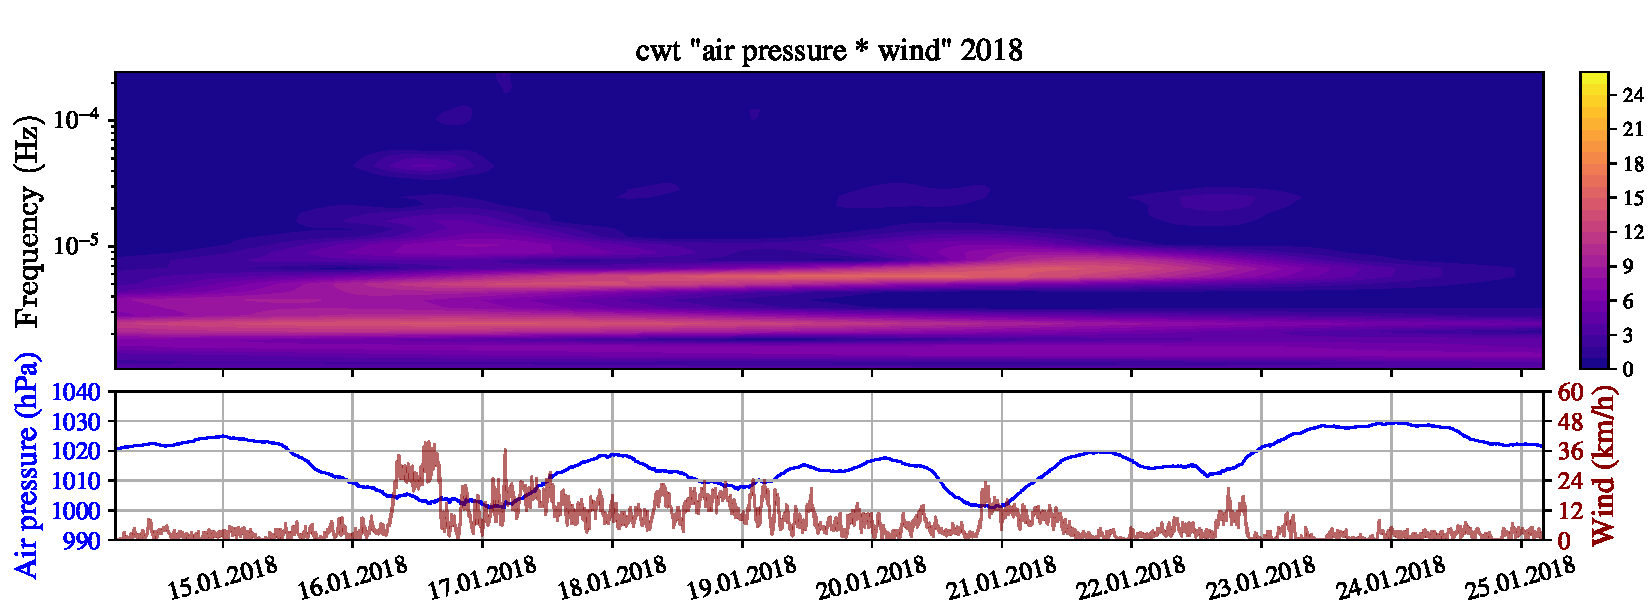
\includegraphics[width=1\textwidth]{papers/wwt/images/storm_airp_wind_zoom2.pdf}
	\caption{Cwt und Rohdaten Strumtief {\em Evi}  und {\em Friedricke} 2018}
	\label{fig:cwt_storm_zoom2}
\end{figure}



\section{Schlussfolgerung}
\rhead{Schlussfolgerung}

Mit dem Versuch, die Wavelet-Transformation im Bereich der Wetteranalyse nützlich anzuwenden, zeigt sich, dass dies durchaus möglich ist.
In der Anwendung mit dem Phänomen der Winterstürme wurde die Wavelet-Transformation oder genauer die stetige Wavelet-Transformation erfolgreich eingesetzt.
Es können zwei Hypothesen aufgestellt werden:
\begin{itemize}
	\item Die periodischen Tagesverläufe bei konstanten Wetterverhältnissen führen dazu, dass die Wavelet-Koeffizienten der \textit{cwt} bei dieser Frequenz deutlich ansteigen (\ref{Freq}).
	
	\item Nicht periodische Ereignisse äussern sich durch das korrelierte Auftreten bei der Betrachtung mehrerer Datenkanäle. Dies kann mit dem Produkt der Wavelet-Koeffizienten oder eben der Kovarianz analysiert werden (\ref{burglind}).
\end{itemize}


Damit ist selbstverständlich noch nichts abschliessend bewiesen. Die Hypothesen müssten detaillierter analysiert werden.
Auch sollte die Methode weiterführend auf andere meteorologische Ereignisse angewandt werden.
Zum Beispiel könnte man versuchen, Gewitter zu detektieren.
Falls sich diese Methode für mehrere Phänomene beweisen lässt, ist eine praktische Anwendung möglich und durchaus vorstellbar. 

\section{Anhang}
Anbei in Abbildung \ref{fig:python-plot-code} und \ref{fig:python-plot-code2} der verwendete Code zum Plotten der Abbildung \ref{fig:cwt_storm}.

\begin{figure}[h]
	\centering
	\lstinputlisting[language=Python,firstline = 1, lastline = 39, numbers=left, firstnumber=1, style = Python]{papers/wwt/code/plot_burglind.py}
	\caption{Python Codeausschnitt}
	\label{fig:python-plot-code}
\end{figure}
\begin{figure}[h]
	\centering
	\lstinputlisting[language=Python,firstline = 40, lastline = 91, firstnumber=40, numbers=left,style = Python]{papers/wwt/code/plot_burglind.py}
	\caption{Python Codeausschnitt}
	\label{fig:python-plot-code2}
\end{figure}
 
 \newpage

\printbibliography[heading=subbibliography]
\end{refsection}

%
% main.tex -- Paper zum Thema wwt
%
% (c) 2019 Michael Schmid, Hochschule Rapperswil
%
\chapter{Wetter-Wavelet-Transformation\label{chapter:wwt}}
\lhead{Wetter-Wavelet-Transformation}
\begin{refsection}
\chapterauthor{Michael Schmid}



\definecolor{codegreen}{rgb}{0,0.6,0}
\definecolor{codegray}{rgb}{0.5,0.5,0.5}
\definecolor{codepurple}{rgb}{0.58,0,0.82}
\definecolor{backcolour}{rgb}{0.95,0.95,0.92}

\lstdefinestyle{mystyle}{
	backgroundcolor=\color{backcolour},   
	commentstyle=\color{codegreen},
	keywordstyle=\color{magenta},
	numberstyle=\tiny\color{codegray},
	stringstyle=\color{codepurple},
	basicstyle=\footnotesize,
	breakatwhitespace=false,         
	breaklines=true,                 
	captionpos=b,                    
	keepspaces=true,                 
	numbers=left,                    
	numbersep=2pt,                  
	showspaces=false,                
	showstringspaces=false,
	showtabs=false,                  
	tabsize=2
}
\lstset{style=mystyle}
\lstdefinestyle{mystyle}{
	morekeywords={cwt,contourf,datetick}
}


\section{Einführung}
\rhead{Einführung}


Seit Langem konsultiere ich meine aktuellen Wetterdaten über eine eher unübliche Internetseite.
Dabei handelt es sich um eine privat geführte Wetterstation, welche die gemessenen Daten im Internet grafisch darstellt.
Die Daten werden auch tabellarisch zur Verfügung gestellt.
Das Feature, welches ich bis anhin am regelmässigsten nutzte, war die grafische Darstellung der aktuellen Wetterdaten über den Zeitraum der letzten 24 Stunden.
Bei speziellen Ereignissen im Wetterverlauf fielen mir besondere und wiederkehrende Charakteristiken auf.
\\

Nach der Einführung in die Theorie der Wavelets kam mir die Idee, solche Wetterphänomene mit einer geeigneten Wavelet Transformation zu detektieren.
In diesem Paper wird einerseits auf die theoretischen Grundlagen der angewandten Methoden zurückgegriffen sowie die besprochenen meteorologischen Phänomene kurz erläutert. 
Weiterführend wird auf die verwendeten Methoden, auch in der praktischen Anwendung, vertieft eingegangen.
Ein besonderes Augenmerk wird auf die allgemeine Vorgehensweise sowie deren Schwierigkeiten gelegt.
\\




\section{Wetterstation Seegräben}
\rhead{Wetterstation Seegräben}

Die angesprochene Wetterstation in der Gemeinde Seegräben im Kanton Zürich ist mit einer DAVIS Vantage Pro2 6153 \cite{online:davisinstruments} realisiert worden.
Sie verfügt über Sensoren für die Temperatur, Feuchtigkeit, Geschwindigkeit und Richtung des Windes sowie für den Niederschlag. 
Durch diese Sensoren werden folgende Daten aufgezeichnet:


\begin{itemize}
	\item \textbf{Aussentemperatur} in Grad Celsius
	\item \textbf{Relative Luftfeuchtigkeit} in Prozent
	\item \textbf{Luftdruck} in hPa
	\item \textbf{Windgeschwindigkeit} in km/h, gemittelt über 5 Minuten
	\item \textbf{Windböen} in km/h
	\item \textbf{Windrichtung} nach Himmelsrichtung
	\item \textbf{Regenmenge} in $\text{l/m}^{2}$
\end{itemize}	


Der Thermo- / Feuchtigkeitssensor liegt zusammen mit dem Regenmengenmesser auf 2 Meter über Boden.
Mit einem Abstand von rund 10 Meter zum nächsten Gebäude sind optimale Messbedingungen geschaffen.
Mit einem Mast ist der Windmesser auf 1.5 Meter über dem First eines Gebäudes lokalisiert \space \cite{online:wss}.
Die Daten werden anschliessend mit einer Software von PC-Wetterstation.de weiterverarbeitet und auf der Website \cite{online:wss} veröffentlicht.
Mehr zur Verwendung der Wetterdaten im n\"achsten Abschnitt.

\section{Datenaufarbeitung}
\rhead{Datenaufarbeitung}
Der n\"achste Vorbereitungsschritt zur Wavelet Transformation war die Aufbereitung der zur Verf\"ugung gestellten Daten der Wetterstation. Dazu musste erst analysiert werden, wie die Daten auf der Website dargestellt werden.
\subsection{Wetter-Archiv}
Auf der Website gibt es mehrere Möglichkeiten, sich Wetterdaten aus der Vergangenheit darstellen zu lassen.
In der Kategorie des Archivs auf der Website kann man die Wetterdaten eines gew\"unschten Zeitraums tabellarisch oder grafisch darstellen lassen.
Vom Betreiber der Website steht keine Funktion zur Verfügung, welche es erlaubt, die Daten offiziell und automatisch herunterzuladen.
\subsection{Datenerfassung}
Da f\"ur die angestrebte Anwendung eine m\"oglichst hohe Aufl\"osung der jeweiligen Daten erforderlich ist, mussten die Daten im Zeitraum von einem Tag dargestellt werden.
Dies hatte zur Folge, dass man f\"ur jeden Tag eine Tabelle auf dem Archiv der Website \"offnen musste. Man hätte anschliessend die Daten mit copy and paste in eine Excel-Tabelle einf\"ugen können. Daher wurde  entschieden, ein Programm zu schreiben, welches diese Aufgabe automatisieren sollte.
Als Programmiersprache wurde hierf\"ur Python gewählt.


Mit der Pandas Library und der Funktion \texttt{'read\_html'} \space konnten die Daten direkt aus dem Python Programm von der Website heruntergeladen werden.
Entscheidend für das Gelingen dieser Teilaufgabe war, dass die URL-Links der einzelnen Tage stets regelmässig aufgebaut sind:
\\
\\
$$\centering{\textit{https://www.wetter-seegraeben.ch/uploads/insert.php?insert=\textbf{20190701}.htm}}$$
\\
Wie zu sehen ist, wird der Link mit dem Datum regelmässig aufgebaut. Somit konnten die entsprechenden Links mit mehreren While-Schleife zusammengesetzt werden.
In der Abbildung \ref{fig:python-code} ist der wesentliche Ausschnitt aus dem Python Code dargestellt.
\begin{figure}
	\centering
	\lstinputlisting[language=Python,firstline=1,lastline=16,numbers=left,style = Python]{papers/wwt/code/get_data.py}
	\caption{Python Codeausschnitt}
	\label{fig:python-code}
\end{figure}
Die Daten konnten im nächsten Schritt in einer Excel-Tabelle abgespeichert werden.
Dort folgte der letzte Feinschliff; d.h. alle überflüssigen Kopfzeilen und Statistiken wurden entfernt.

\subsubsection{Unregelmässigkeiten der Wetterstation}
Bei der Datenerfassung durch das eben beschriebene Python Programm wurden einige Unregelmässigkeiten der Wetterstation beobachtet.
Das Programm wird jeweils durch eine Fehlermeldung abgebrochen, wenn der angegebene Link nicht abrufbar ist. 
So fiel auf, dass unregelmässig auf das Jahr verteilt, Daten von gewissen Tagen fehlten. Es stellte sich heraus, dass hinter dem eigentlich korrektem Link die entsprechende Internetseite nicht zur Verfügung steht.
Wird manuell auf der Website nach diesem Tag gesucht, kann nichts gefunden werden.
Dies trat teilweise sogar in Abschnitten von mehreren Tagen auf.
Wie sich später herausstellte, traten die fehlenden Tagen nicht zu den Zeitpunkten auf, die mich interessierten.


\subsection{Datendarstellung}
Die Darstellung der gewonnenen Daten konnte einfach mittels Python realisiert werden.
Anbei in Abbildung \ref{fig:rawdata} der Plot der Rohdaten aus dem Jahre 2018, wobei nur jeder zehnte Messpunkt verwendet wurde.
Diese Rohdaten dienten als Grundlage für alle weiteren Berechnungen. 
\begin{figure}
	\centering
	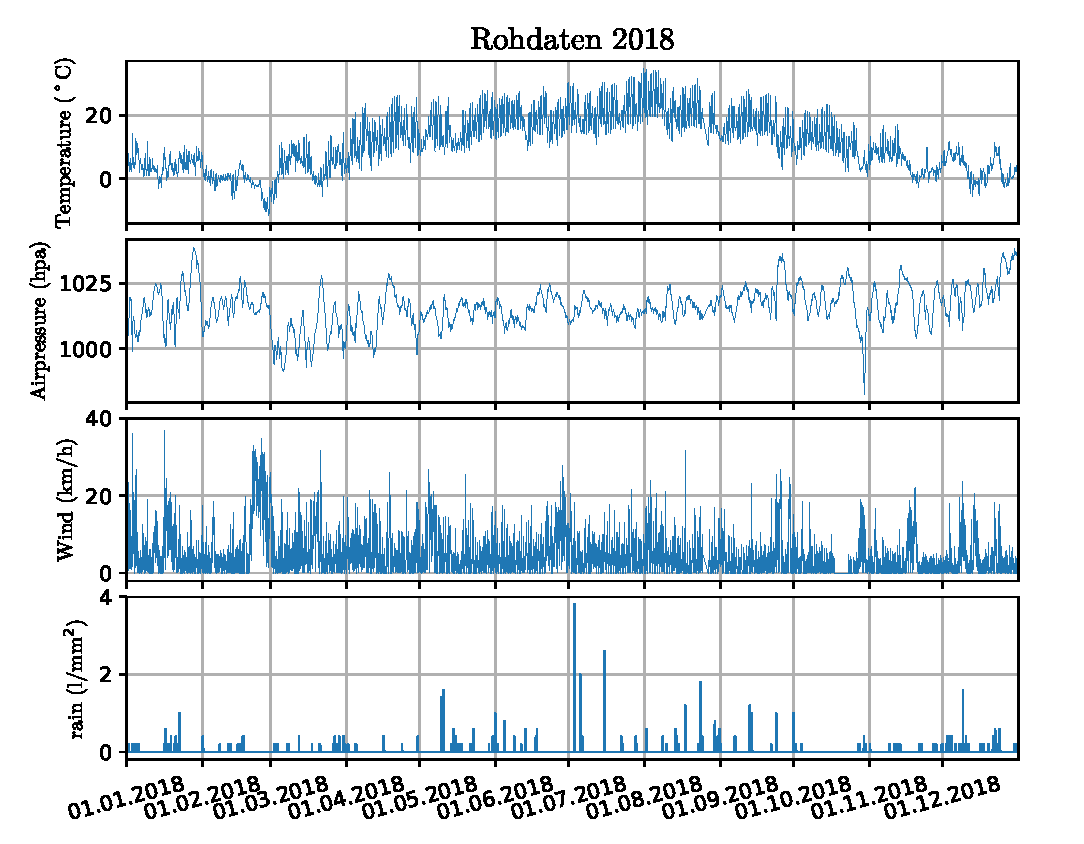
\includegraphics[width=1\textwidth]{papers/wwt/images/raw.pdf}
	\caption{Rohdaten 2018}
	\label{fig:rawdata}
\end{figure}


\section{Stetige Wavelet-Transformation}
\rhead{Stetige Wavelet-Transformation}
Die theoretischen Grundlagen rund um die stetige Wavelet-Transformation wurden im Kapitel \ref{chapter:cwt} genaustens erläutert. 
In diesem Abschnitt der Seminararbeit wird öfters auf die Theorie des angesprochenen Kapitels \ref{chapter:cwt} referenziert ohne diese genauer zu erläutern. 

Für eine m"oglichst aussagekräftige Untersuchung der Signale, in welcher so viele Informationen gewonnen werden sollten wie m"oglich, eignet sich die stetige Wavelet-Transformation (folgend noch kurz \textit{cwt} aus dem Englischen "continuous wavelet transform"). 
Regelmässig auftretende Frequenzen können dank der \textit{cwt} gefunden und zusätzlich einem Zeitraum zugeordnet werden.
\subsection{Das verwendete Wavelet}
In
\begin{equation}
\mathcal{W}f (a,b)
=
\langle f,\psi_{a,b}\rangle
=
\frac{1}{\sqrt{|a|}}\int_{-\infty}^\infty f(t)\,\overline{
	\psi\biggl(\frac{t-b}{a}\biggr)}\,dt
\label{eq:cwt1}
\end{equation}
erkennt man die grundlegende Formel der \textit{cwt}.
Wobei das $\psi_{a,b}$ für das Mutter-Wavelet steht, welches mit dem Koeffizienten $a$ skaliert und mit $b$ verschoben wird.

Als Mutter-Wavelet wurde 
\begin{equation}
\psi_{Gabor}(t) =  c_{\sigma} e^{-\frac{1}{2}t^2} \biggl(e^{i \sigma t}- e^{-\frac{1}{2} \sigma^2} \biggr)
\label{eq:morlet}
\end{equation} \cite{online:Morlet}
verwendet, welches auch als das analytische Gabor-Wavelet bekannt ist.
Dabei gibt $\sigma$ an, wie hoch die Frequenz ist und dementsprechend auch, wie viele lokale Maxima und Minima innerhalb des Gauss'schen Fensters das Mutter-Wavelet existieren.
Weiter ist $c_{\sigma}$ eine reelle Konstante und dient zur Erf"ullung der Zulässigkeitsbedingungen in der Definition \ref{cwt:zulaessig}.
Das Morlet-Wavelet wird in der Abbildung \ref{fig:gabor_plot} \space dargestellt und $\sigma$ wurde auf 5 gesetzt.

\begin{figure}
\centering
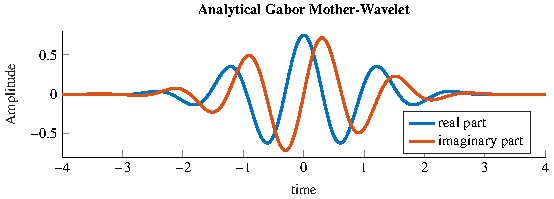
\includegraphics[width=1\textwidth]{papers/wwt/images/gabor.pdf}
\caption{Analytisches Gabor Mutter-Wavelet}
\label{fig:gabor_plot}
\end{figure}

Weiter ist zu erwähnen, dass das eben gezeigte Gabor Wavelet der referenzierten Quelle entnommen wurde. Ob Matlab die selbe Form verwendet, konnte nicht abschliessend geklärt werden.

\subsection{Berechung mit Matlab}
Die Berechnung der \textit{cwt} wurde mit der numerischen Berechnungs-Software Matlab durchgeführt.
Die dafür verwendete Funktion war die cwt()-Funktion.
Die Funktion arbeitete bei korrekter Parametrisierung wie gewünscht.
Falls man verstehen möchte wie die Funktion genau rechnet, muss man sich mit einer eher dürftigen Dokumentation herumschlagen.
Folgende Parameter wurden verwendet
\lstinputlisting[language=Matlab,firstline=1,lastline=1,  numbers=left, style = mystyle]{papers/wwt/code/matlab.m}
\label{fig:matlab_code_cwt}
wobei Matlab das Gabor-Wavelet als \texttt{'amor'} bezeichnet, mit \texttt{'VoicesPerOctave'} konnte die Genauigkeit erhöht werden und die Variable \texttt{'fs'} beschreibt die Abtastfrequenz der Messsignale.
Bei den Rückgabewerten werden die Wavelet-Werte in \texttt{'wt'} als komplexe Matrix und die approximierten Frequenzen in \texttt{'F'} abgespeichert.

Anstelle des Skalierungsfaktors $a$ in der Gleichung \ref{eq:cwt} berechnet Matlab eine approximierte Frequenz und gibt diese zurück.
Für jeden verwendeten Skalierungsfaktor $a$ wird eine Sinuskurve gesucht, die am ehesten mit der Frequenz des entsprechenden Wavelets übereinstimmt.
Siehe das Beispiel mit einem Daubechies Wavelet der Nummer 7 in der Abbildung \ref{fig:centerf}.
Dies dient dazu den Wavelet-Koeffizienten einer Frequenz zuzuordnen. 
Aus dem verwendeten Skalierungsfaktor $a$ könnte auf die Schnelle keine Information entnommen werden.
\begin{figure}[h]
	\centering
	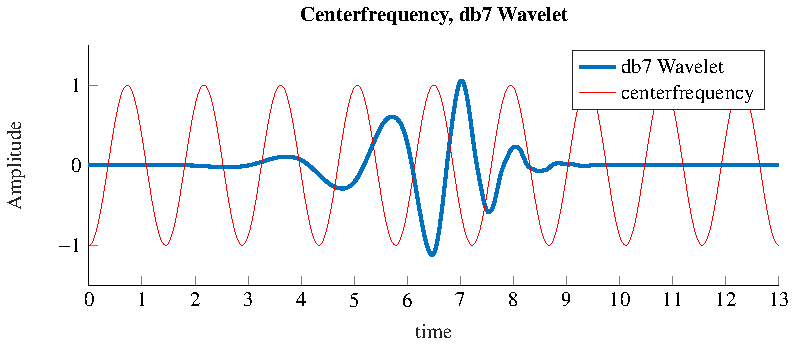
\includegraphics[width=1\textwidth]{papers/wwt/images/centerf.pdf}
	\caption{Approximierte Frequenz eines db7-Wavelet}
	\label{fig:centerf}
\end{figure}

\subsection{Verifikation der approximierten Frequenz}
\label{Freq}
Diese approximierte Frequenz konnte man mit den geeigneten Daten aus der aktuellen Anwendung der Wetterdaten sehr gut verifizieren.
Der Temperaturverlauf während einer Hochdruckphase ist sehr regelmässig und man sollte den 24 Stunden Tagesverlauf exakt erkennen.

Dank der Regelm"assigkeit des Temperaturverlaufs sieht man im \textit{cwt}-Plot eine Erh"ohung des Wertes bei einer gewissen Frequenz.
Die ausgelesene Frequenz beträgt $f = 1.16\cdot10^{-5} \,\text{Hz}$, die umgerechnet einer Periodendauer von $T = 86206.897\,\text{s}\approx 23\,\text{h }56\,\text{min } 47\,\text{s}$ entspricht.
Damit kann die Frequenz im Rückgabewert der Matlab-Funktion als sehr genau bezeichnet werden.
Dabei kommt weiter dazu, dass nur alle f"unf Minuten ein Datenpunkt aufgenommen wurde und somit die Abweichung zu 24 Stunden kleiner ist als die eigentliche Auflösung.

\begin{figure}[h]
	\centering
	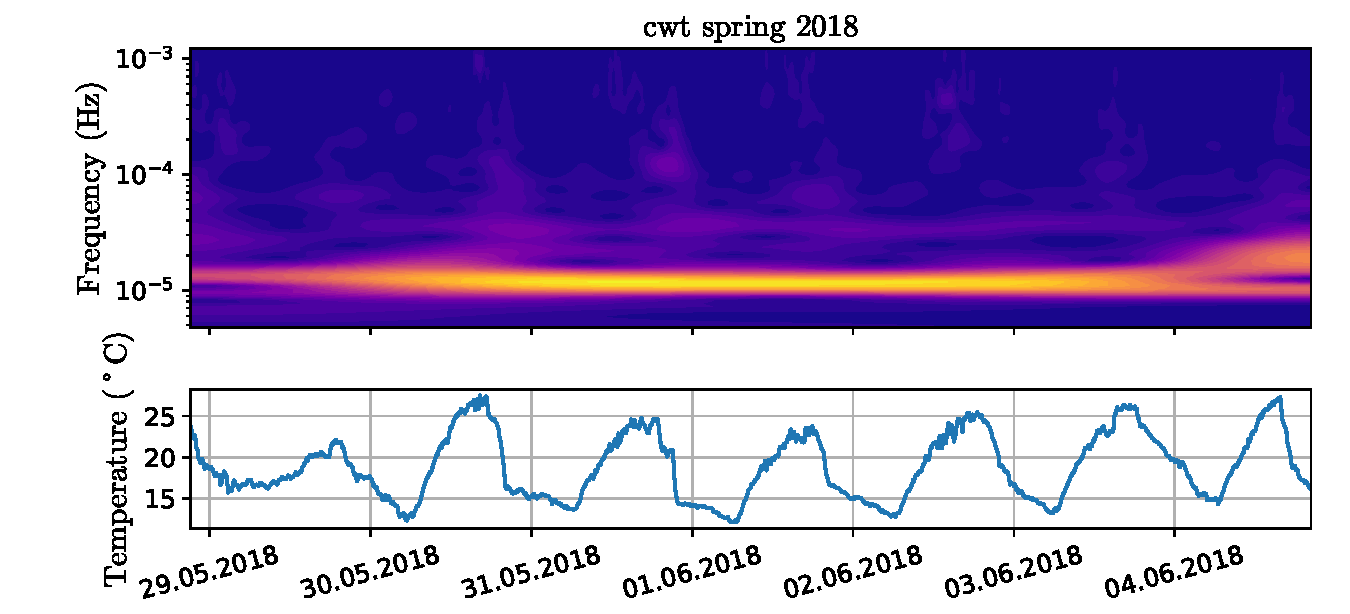
\includegraphics[width=1\textwidth]{papers/wwt/images/data_spring.pdf}
	\caption{Temperaturverlauf und entsprechende cwt}
	\label{fig:cwt_zoom}
\end{figure}



\section{Analyse von Wettereignissen}
\rhead{Analyse von Wetterereignissen}
Aufgrund der Kenntnisse rund um die \textit{cwt} kann angenommen werden, dass ein Wechsel in der Frequenz gut detektiert werden kann.
Bei einer typischen Sturmfront, welche öfters als Wintersturm in den Monaten Dezember und Januar auftreten, zeigten sich bei der Konsultation der Wetterdaten rapide Temperatur- und Luftdruckwechsel sowie ein erhöhtes Windaufkommen.
Das Ziel der Analyse war, solche Ereignisse mittels einer geeigneten \textit{cwt} zu detektieren.
Bei den Rohdaten der Frontdurchgängen erkennt man gemeinsame Wechsel im Wind, der Temperatur sowie dem Luftdruck, daher kann in der Wavelet-Transformation eine erkennbare Antwort erwartet werden. 
Diese korrelierenden auftretenden Frequenzen sollten in der \textit{cwt} sichtbar sein.

\subsection{Parallelen zur Kovarianz}

Um das korrelierende Auftreten der einzelnen Datenkanäle zu verdeutlichen, wurden bei diesen jeweils die zwei zusammengehörenden Koeffizienten der \textit{cwt} miteinander multipliziert. 
Dabei werden die Stellen hervorgehoben, wo beispielsweise der Luftdruck und die Windgeschwindigkeit abhängig voneinander variieren.  
Dies funktioniert besonders gut, da die Werte rasch gegen null gehen falls nur schon einer der beiden Datenverläufe nicht mit dem aktuellen Mutter-Wavelet übereinstimmt.
Genauer betrachtet zeigt dieses Verfahren Ähnlichkeiten mit der Formel
\begin{equation}
COV(X,Y) = \frac{\sum_{i=1}^{N} (x_i- \bar{x})(y_i- \bar{y})}{N-1},
\label{eq:kovarianz}
\end{equation}
der Kovarianz aus der Statistik. Bei dieser Anwendung wird einfach nicht die ganze Zufallsvariable benutzt, sondern nur jeweils die beiden zeitlich übereinstimmenden Werte.

Die Kovarianz zeigt sich nicht nur in dieser Anwendung. Auch schon bei der grundlegenden Formel \ref{eq:cwt1} der \textit{cwt}, kann man gewisse Parallelen sehen. 
In \ref{eq:cwt1} ist die Motivation, die jeweiligen Parameter $a$ und $b$ zu finden, wobei das Mutter-Wavelet und das Signal gemeinsam variieren.
Auch hierfür werden die Produkte der Signale berechnet, auf integriert und gemittelt.
Auch dies ist eine etwas abgewandelte Art der Kovarianz zwischen dem Datensignal und dem Mutter-Wavelet.


Die im Paper angewendete Wavelet-Transformation mit der Idee des Produktes der beiden Datenkanäle,
\begin{equation}
\begin{split}
\mathcal{W}f (a,b)
& =
\biggl<\langle Luftdruck,\psi_{a,b}\rangle, \langle Wind,\psi_{a,b} \rangle \biggr > \\
& = \biggl< \frac{1}{\sqrt{|a|}}\int_{-\infty}^\infty Luftdruck(t)\,\overline{
	\psi\biggl(\frac{t-b}{a}\biggr)}\,dt
,
\frac{1}{\sqrt{|a|}}\int_{-\infty}^\infty Wind(t)\,\overline{
	\psi\biggl(\frac{t-b}{a}\biggr)}\,dt \biggr>
\label{eq:cwt_wwt}
\end{split}
\end{equation}
kann, vorerst nur für den Luftdruck, auf die Kovarianz (Formel \ref{eq:kovarianz}) umgeschrieben werden,

\begin{equation}
COV(Luftdruck, \psi_{a,b})f(a,b) = \frac{\sum_{i=1}^{N} (Luftdruck_i - \overline{Luftdruck})(\psi_{a,b}-  \overline{\psi_{a,b}})}{N-1}.
\end{equation}
Gemäss den Zulässigkeitsbedingungen eines Mutter-Wavelets ist $\overline{\psi_{a,b}} = 0$ (Definition \ref{cwt:zulaessig}). Weiter werden Multiplikationen in Skalarprodukte umgewandelt, somit folgt;
\begin{equation}
COV(Luftdruck, \psi_{a,b})f(a,b) =  \frac{\sum_{i=1}^{N} 
 \langle Luftdruck_i- \overline{Luftdruck},\psi_{a,b}\rangle}{N-1}.
\end{equation}
Weiter Ausmultipliziert
\begin{equation}
COV(Luftdruck, \psi_{a,b})f(a,b) = \frac{\sum_{i=1}^{N} 
\langle Luftdruck_i,\psi_{a,b}\rangle - \langle \overline{Luftdruck},\psi_{a,b}\rangle}{N-1},
\end{equation}
schlussendlich ergibt sich mit $\langle \overline{Luftdruck},\psi_{a,b} \rangle = 0$,
\begin{equation}
COV(Luftdruck, \psi_{a,b})f(a,b) = \frac{\sum_{i=1}^{N} 
	\langle Luftdruck_i,\psi_{a,b}\rangle}{N-1}.
\end{equation}
 Wird noch das Produkt mit dem Wind hinzugenommen
 \begin{equation}
 \begin{split}
\biggl< COV(Luftdruck, \psi_{a,b})f(a,b), COV(Wind), \psi_{a,b})f(a,b) \biggr > \\
=
 \biggl< \frac{\sum_{i=1}^{N} 
 	\langle Luftdruck_i,\psi_{a,b}\rangle}{N-1},\frac{\sum_{i=1}^{N} 
 	\langle Wind_i,\psi_{a,b}\rangle}{N-1} \biggr >,
 \label{eq:cov_wwt}
 \end{split}
 \end{equation}
 wurde die Herleitung von der Wavelet-Transformation in der Formel \ref{eq:cwt_wwt} zum einem äquivalenten Resultat, ohne die Korrekturfaktoren, mit der Kovarianz in der Formel \ref{eq:cov_wwt} gezeigt.



\subsection{Sturmsaison 2018}
\rhead{Sturmsaison 2018}
Bereits bekannt war, dass in der Sturmsaison im Jahre 2018 einige heftige Winterstürme aufgetreten sind.
So wurde bei der Analyse der Daten nur auf diese Periode das Augenmerk gelegt. 
In Abbildung \ref{fig:cwt_storm} \space sieht man die Wavelet-Transformation des Luftdruckes und Windes miteinander multipliziert.
Dies über die Monate Januar und Februar im Jahre 2018 hinweg.
Weiter wird der Luftdruck- und Windverlauf dargestellt.
 
\begin{figure}[h]
	\centering
	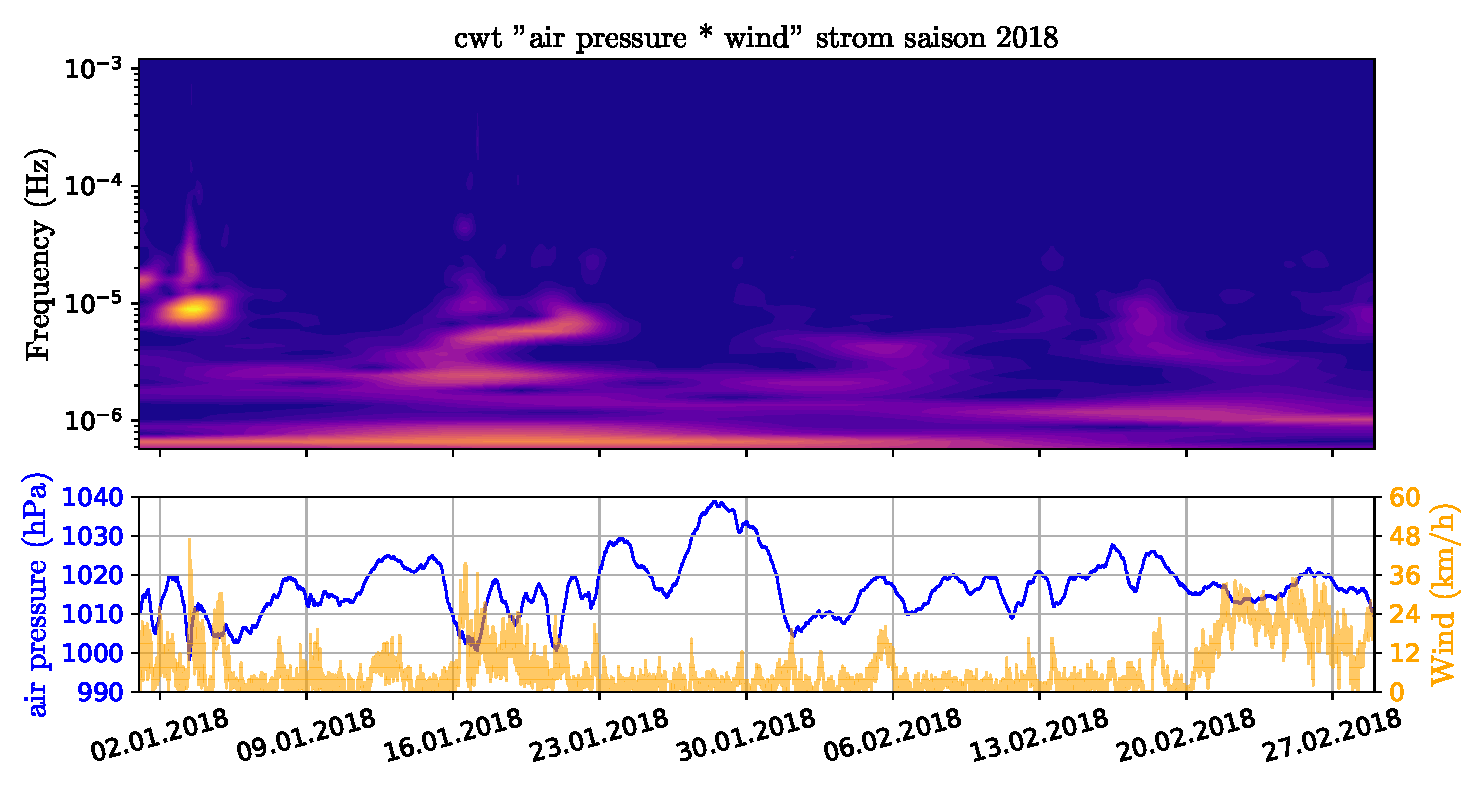
\includegraphics[width=1\textwidth]{papers/wwt/images/storm_airp_wind.pdf}
	\caption{Cwt und Rohdaten Sturmsaison 2018}
	\label{fig:cwt_storm}
\end{figure}

In Abbildung \ref{fig:cwt_storm} \space zeigen sich um den 3. sowie zwischen dem 16. und 23. Januar jeweils gewisse Frequenzen des Windes und des Luftdruckes, die gemeinsam auf die Wavelet-Transformation angesprochen haben.

\subsubsection{Wintersturm {\em Burglind} }
\label{burglind}
Hineingezoomt um den 3. Januar (Abbildung \ref{fig:cwt_storm_zoom}) sind im Rohdatenverlauf die Aktivitäten des Windes und Luftdruckes erkennbar. 
\begin{figure}[b]
	\centering
	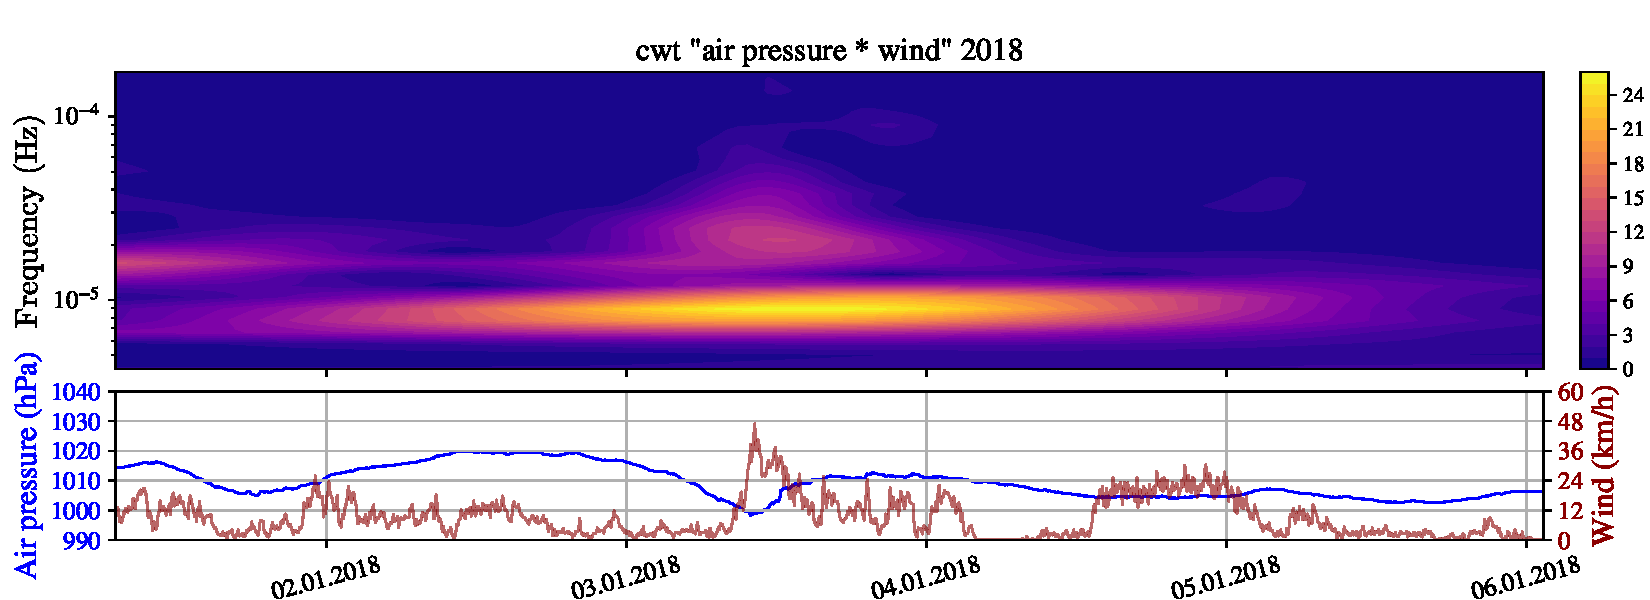
\includegraphics[width=1\textwidth]{papers/wwt/images/storm_airp_wind_zoom.pdf}
	\caption{Cwt und Rohdaten Wintersturm {\em Burglind}  2018}
	\label{fig:cwt_storm_zoom}
\end{figure}
Aus dem Fachbericht \space \cite{Fachbericht:Burglind} von Meteoschweiz war bekannt, dass am Vormittag des 3. Januars 2018 die stärkste Sturmfront seit dem verheerenden Sturm Lothar aus dem Jahre 1999 über die Schweiz zog.
Dabei zeigt sich eindrücklich, wie der Sturmdurchgang in der multiplizierten Wavelet-Transformation hervorgehoben wird.

\subsubsection{Sturmtief {\em Evi}  und {\em Friedricke} }
\label{evi}
Beim zweiten Ereignis zwischen dem 16. und 23. Januar trat die Aktivität nicht mehr so deutlich auf.
Nach dem Sturmarchiv  \cite{online:sturmarchiv} traf am 16. Januar das Sturmtief {\em Evi}  und am 18. Januar das Sturmtief {\em Friedricke} auf Europa. Dabei zeigt sich nach der Amplitude, dass das Sturmtief nicht direkt auf die Schweiz traf, sonder diese lediglich streifte. 

\begin{figure}[h]
	\centering
	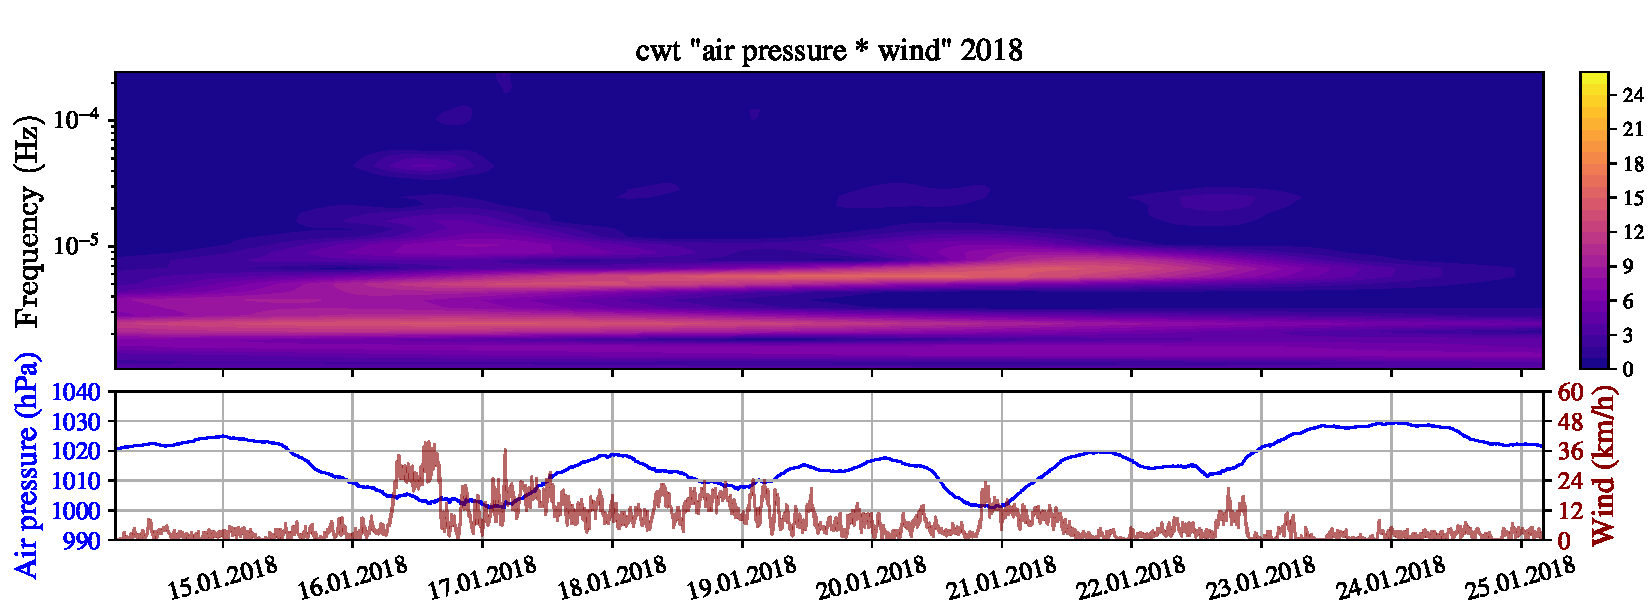
\includegraphics[width=1\textwidth]{papers/wwt/images/storm_airp_wind_zoom2.pdf}
	\caption{Cwt und Rohdaten Strumtief {\em Evi}  und {\em Friedricke} 2018}
	\label{fig:cwt_storm_zoom2}
\end{figure}



\section{Schlussfolgerung}
\rhead{Schlussfolgerung}

Mit dem Versuch, die Wavelet-Transformation im Bereich der Wetteranalyse nützlich anzuwenden, zeigt sich, dass dies durchaus möglich ist.
In der Anwendung mit dem Phänomen der Winterstürme wurde die Wavelet-Transformation oder genauer die stetige Wavelet-Transformation erfolgreich eingesetzt.
Es können zwei Hypothesen aufgestellt werden:
\begin{itemize}
	\item Die periodischen Tagesverläufe bei konstanten Wetterverhältnissen führen dazu, dass die Wavelet-Koeffizienten der \textit{cwt} bei dieser Frequenz deutlich ansteigen (\ref{Freq}).
	
	\item Nicht periodische Ereignisse äussern sich durch das korrelierte Auftreten bei der Betrachtung mehrerer Datenkanäle. Dies kann mit dem Produkt der Wavelet-Koeffizienten oder eben der Kovarianz analysiert werden (\ref{burglind}).
\end{itemize}


Damit ist selbstverständlich noch nichts abschliessend bewiesen. Die Hypothesen müssten detaillierter analysiert werden.
Auch sollte die Methode weiterführend auf andere meteorologische Ereignisse angewandt werden.
Zum Beispiel könnte man versuchen, Gewitter zu detektieren.
Falls sich diese Methode für mehrere Phänomene beweisen lässt, ist eine praktische Anwendung möglich und durchaus vorstellbar. 

\section{Anhang}
Anbei in Abbildung \ref{fig:python-plot-code} und \ref{fig:python-plot-code2} der verwendete Code zum Plotten der Abbildung \ref{fig:cwt_storm}.

\begin{figure}[h]
	\centering
	\lstinputlisting[language=Python,firstline = 1, lastline = 39, numbers=left, firstnumber=1, style = Python]{papers/wwt/code/plot_burglind.py}
	\caption{Python Codeausschnitt}
	\label{fig:python-plot-code}
\end{figure}
\begin{figure}[h]
	\centering
	\lstinputlisting[language=Python,firstline = 40, lastline = 91, firstnumber=40, numbers=left,style = Python]{papers/wwt/code/plot_burglind.py}
	\caption{Python Codeausschnitt}
	\label{fig:python-plot-code2}
\end{figure}
 
 \newpage

\printbibliography[heading=subbibliography]
\end{refsection}

%
% main.tex -- Paper zum Thema wwt
%
% (c) 2019 Michael Schmid, Hochschule Rapperswil
%
\chapter{Wetter-Wavelet-Transformation\label{chapter:wwt}}
\lhead{Wetter-Wavelet-Transformation}
\begin{refsection}
\chapterauthor{Michael Schmid}



\definecolor{codegreen}{rgb}{0,0.6,0}
\definecolor{codegray}{rgb}{0.5,0.5,0.5}
\definecolor{codepurple}{rgb}{0.58,0,0.82}
\definecolor{backcolour}{rgb}{0.95,0.95,0.92}

\lstdefinestyle{mystyle}{
	backgroundcolor=\color{backcolour},   
	commentstyle=\color{codegreen},
	keywordstyle=\color{magenta},
	numberstyle=\tiny\color{codegray},
	stringstyle=\color{codepurple},
	basicstyle=\footnotesize,
	breakatwhitespace=false,         
	breaklines=true,                 
	captionpos=b,                    
	keepspaces=true,                 
	numbers=left,                    
	numbersep=2pt,                  
	showspaces=false,                
	showstringspaces=false,
	showtabs=false,                  
	tabsize=2
}
\lstset{style=mystyle}
\lstdefinestyle{mystyle}{
	morekeywords={cwt,contourf,datetick}
}


\section{Einführung}
\rhead{Einführung}


Seit Langem konsultiere ich meine aktuellen Wetterdaten über eine eher unübliche Internetseite.
Dabei handelt es sich um eine privat geführte Wetterstation, welche die gemessenen Daten im Internet grafisch darstellt.
Die Daten werden auch tabellarisch zur Verfügung gestellt.
Das Feature, welches ich bis anhin am regelmässigsten nutzte, war die grafische Darstellung der aktuellen Wetterdaten über den Zeitraum der letzten 24 Stunden.
Bei speziellen Ereignissen im Wetterverlauf fielen mir besondere und wiederkehrende Charakteristiken auf.
\\

Nach der Einführung in die Theorie der Wavelets kam mir die Idee, solche Wetterphänomene mit einer geeigneten Wavelet Transformation zu detektieren.
In diesem Paper wird einerseits auf die theoretischen Grundlagen der angewandten Methoden zurückgegriffen sowie die besprochenen meteorologischen Phänomene kurz erläutert. 
Weiterführend wird auf die verwendeten Methoden, auch in der praktischen Anwendung, vertieft eingegangen.
Ein besonderes Augenmerk wird auf die allgemeine Vorgehensweise sowie deren Schwierigkeiten gelegt.
\\




\section{Wetterstation Seegräben}
\rhead{Wetterstation Seegräben}

Die angesprochene Wetterstation in der Gemeinde Seegräben im Kanton Zürich ist mit einer DAVIS Vantage Pro2 6153 \cite{online:davisinstruments} realisiert worden.
Sie verfügt über Sensoren für die Temperatur, Feuchtigkeit, Geschwindigkeit und Richtung des Windes sowie für den Niederschlag. 
Durch diese Sensoren werden folgende Daten aufgezeichnet:


\begin{itemize}
	\item \textbf{Aussentemperatur} in Grad Celsius
	\item \textbf{Relative Luftfeuchtigkeit} in Prozent
	\item \textbf{Luftdruck} in hPa
	\item \textbf{Windgeschwindigkeit} in km/h, gemittelt über 5 Minuten
	\item \textbf{Windböen} in km/h
	\item \textbf{Windrichtung} nach Himmelsrichtung
	\item \textbf{Regenmenge} in $\text{l/m}^{2}$
\end{itemize}	


Der Thermo- / Feuchtigkeitssensor liegt zusammen mit dem Regenmengenmesser auf 2 Meter über Boden.
Mit einem Abstand von rund 10 Meter zum nächsten Gebäude sind optimale Messbedingungen geschaffen.
Mit einem Mast ist der Windmesser auf 1.5 Meter über dem First eines Gebäudes lokalisiert \space \cite{online:wss}.
Die Daten werden anschliessend mit einer Software von PC-Wetterstation.de weiterverarbeitet und auf der Website \cite{online:wss} veröffentlicht.
Mehr zur Verwendung der Wetterdaten im n\"achsten Abschnitt.

\section{Datenaufarbeitung}
\rhead{Datenaufarbeitung}
Der n\"achste Vorbereitungsschritt zur Wavelet Transformation war die Aufbereitung der zur Verf\"ugung gestellten Daten der Wetterstation. Dazu musste erst analysiert werden, wie die Daten auf der Website dargestellt werden.
\subsection{Wetter-Archiv}
Auf der Website gibt es mehrere Möglichkeiten, sich Wetterdaten aus der Vergangenheit darstellen zu lassen.
In der Kategorie des Archivs auf der Website kann man die Wetterdaten eines gew\"unschten Zeitraums tabellarisch oder grafisch darstellen lassen.
Vom Betreiber der Website steht keine Funktion zur Verfügung, welche es erlaubt, die Daten offiziell und automatisch herunterzuladen.
\subsection{Datenerfassung}
Da f\"ur die angestrebte Anwendung eine m\"oglichst hohe Aufl\"osung der jeweiligen Daten erforderlich ist, mussten die Daten im Zeitraum von einem Tag dargestellt werden.
Dies hatte zur Folge, dass man f\"ur jeden Tag eine Tabelle auf dem Archiv der Website \"offnen musste. Man hätte anschliessend die Daten mit copy and paste in eine Excel-Tabelle einf\"ugen können. Daher wurde  entschieden, ein Programm zu schreiben, welches diese Aufgabe automatisieren sollte.
Als Programmiersprache wurde hierf\"ur Python gewählt.


Mit der Pandas Library und der Funktion \texttt{'read\_html'} \space konnten die Daten direkt aus dem Python Programm von der Website heruntergeladen werden.
Entscheidend für das Gelingen dieser Teilaufgabe war, dass die URL-Links der einzelnen Tage stets regelmässig aufgebaut sind:
\\
\\
$$\centering{\textit{https://www.wetter-seegraeben.ch/uploads/insert.php?insert=\textbf{20190701}.htm}}$$
\\
Wie zu sehen ist, wird der Link mit dem Datum regelmässig aufgebaut. Somit konnten die entsprechenden Links mit mehreren While-Schleife zusammengesetzt werden.
In der Abbildung \ref{fig:python-code} ist der wesentliche Ausschnitt aus dem Python Code dargestellt.
\begin{figure}
	\centering
	\lstinputlisting[language=Python,firstline=1,lastline=16,numbers=left,style = Python]{papers/wwt/code/get_data.py}
	\caption{Python Codeausschnitt}
	\label{fig:python-code}
\end{figure}
Die Daten konnten im nächsten Schritt in einer Excel-Tabelle abgespeichert werden.
Dort folgte der letzte Feinschliff; d.h. alle überflüssigen Kopfzeilen und Statistiken wurden entfernt.

\subsubsection{Unregelmässigkeiten der Wetterstation}
Bei der Datenerfassung durch das eben beschriebene Python Programm wurden einige Unregelmässigkeiten der Wetterstation beobachtet.
Das Programm wird jeweils durch eine Fehlermeldung abgebrochen, wenn der angegebene Link nicht abrufbar ist. 
So fiel auf, dass unregelmässig auf das Jahr verteilt, Daten von gewissen Tagen fehlten. Es stellte sich heraus, dass hinter dem eigentlich korrektem Link die entsprechende Internetseite nicht zur Verfügung steht.
Wird manuell auf der Website nach diesem Tag gesucht, kann nichts gefunden werden.
Dies trat teilweise sogar in Abschnitten von mehreren Tagen auf.
Wie sich später herausstellte, traten die fehlenden Tagen nicht zu den Zeitpunkten auf, die mich interessierten.


\subsection{Datendarstellung}
Die Darstellung der gewonnenen Daten konnte einfach mittels Python realisiert werden.
Anbei in Abbildung \ref{fig:rawdata} der Plot der Rohdaten aus dem Jahre 2018, wobei nur jeder zehnte Messpunkt verwendet wurde.
Diese Rohdaten dienten als Grundlage für alle weiteren Berechnungen. 
\begin{figure}
	\centering
	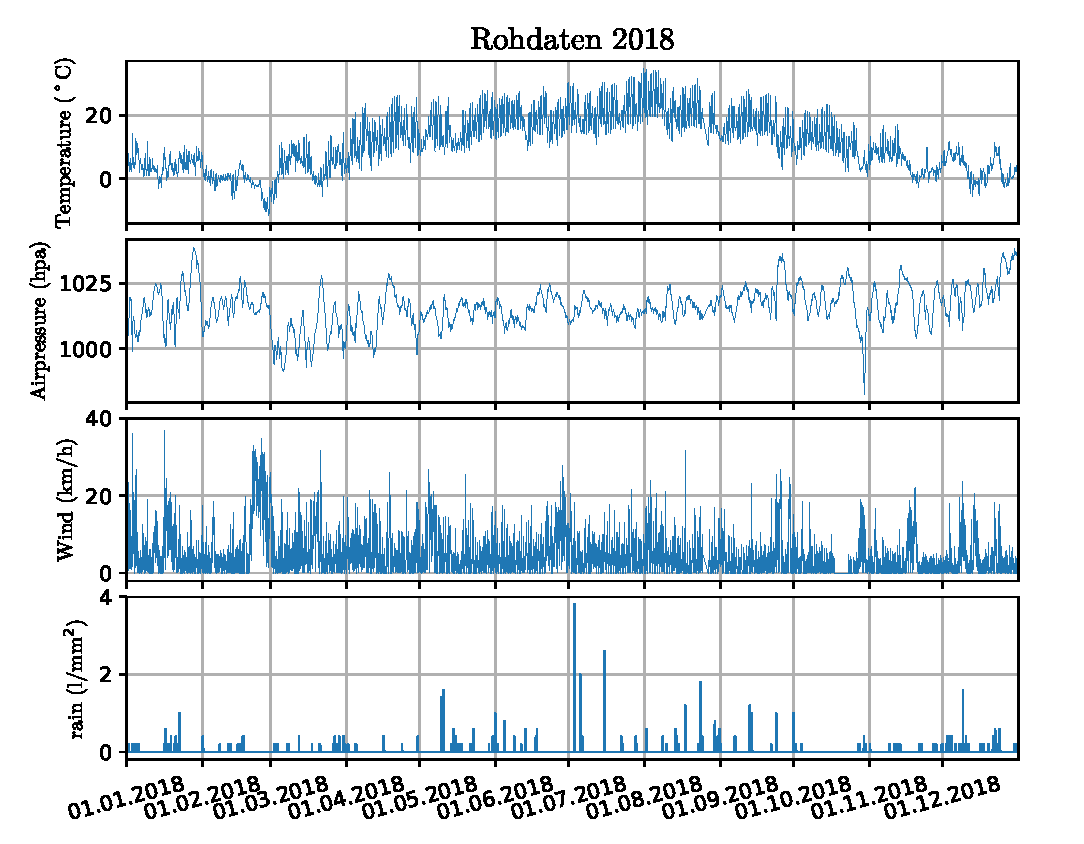
\includegraphics[width=1\textwidth]{papers/wwt/images/raw.pdf}
	\caption{Rohdaten 2018}
	\label{fig:rawdata}
\end{figure}


\section{Stetige Wavelet-Transformation}
\rhead{Stetige Wavelet-Transformation}
Die theoretischen Grundlagen rund um die stetige Wavelet-Transformation wurden im Kapitel \ref{chapter:cwt} genaustens erläutert. 
In diesem Abschnitt der Seminararbeit wird öfters auf die Theorie des angesprochenen Kapitels \ref{chapter:cwt} referenziert ohne diese genauer zu erläutern. 

Für eine m"oglichst aussagekräftige Untersuchung der Signale, in welcher so viele Informationen gewonnen werden sollten wie m"oglich, eignet sich die stetige Wavelet-Transformation (folgend noch kurz \textit{cwt} aus dem Englischen "continuous wavelet transform"). 
Regelmässig auftretende Frequenzen können dank der \textit{cwt} gefunden und zusätzlich einem Zeitraum zugeordnet werden.
\subsection{Das verwendete Wavelet}
In
\begin{equation}
\mathcal{W}f (a,b)
=
\langle f,\psi_{a,b}\rangle
=
\frac{1}{\sqrt{|a|}}\int_{-\infty}^\infty f(t)\,\overline{
	\psi\biggl(\frac{t-b}{a}\biggr)}\,dt
\label{eq:cwt1}
\end{equation}
erkennt man die grundlegende Formel der \textit{cwt}.
Wobei das $\psi_{a,b}$ für das Mutter-Wavelet steht, welches mit dem Koeffizienten $a$ skaliert und mit $b$ verschoben wird.

Als Mutter-Wavelet wurde 
\begin{equation}
\psi_{Gabor}(t) =  c_{\sigma} e^{-\frac{1}{2}t^2} \biggl(e^{i \sigma t}- e^{-\frac{1}{2} \sigma^2} \biggr)
\label{eq:morlet}
\end{equation} \cite{online:Morlet}
verwendet, welches auch als das analytische Gabor-Wavelet bekannt ist.
Dabei gibt $\sigma$ an, wie hoch die Frequenz ist und dementsprechend auch, wie viele lokale Maxima und Minima innerhalb des Gauss'schen Fensters das Mutter-Wavelet existieren.
Weiter ist $c_{\sigma}$ eine reelle Konstante und dient zur Erf"ullung der Zulässigkeitsbedingungen in der Definition \ref{cwt:zulaessig}.
Das Morlet-Wavelet wird in der Abbildung \ref{fig:gabor_plot} \space dargestellt und $\sigma$ wurde auf 5 gesetzt.

\begin{figure}
\centering
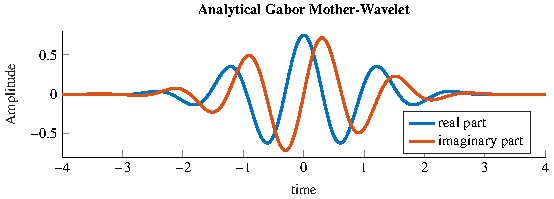
\includegraphics[width=1\textwidth]{papers/wwt/images/gabor.pdf}
\caption{Analytisches Gabor Mutter-Wavelet}
\label{fig:gabor_plot}
\end{figure}

Weiter ist zu erwähnen, dass das eben gezeigte Gabor Wavelet der referenzierten Quelle entnommen wurde. Ob Matlab die selbe Form verwendet, konnte nicht abschliessend geklärt werden.

\subsection{Berechung mit Matlab}
Die Berechnung der \textit{cwt} wurde mit der numerischen Berechnungs-Software Matlab durchgeführt.
Die dafür verwendete Funktion war die cwt()-Funktion.
Die Funktion arbeitete bei korrekter Parametrisierung wie gewünscht.
Falls man verstehen möchte wie die Funktion genau rechnet, muss man sich mit einer eher dürftigen Dokumentation herumschlagen.
Folgende Parameter wurden verwendet
\lstinputlisting[language=Matlab,firstline=1,lastline=1,  numbers=left, style = mystyle]{papers/wwt/code/matlab.m}
\label{fig:matlab_code_cwt}
wobei Matlab das Gabor-Wavelet als \texttt{'amor'} bezeichnet, mit \texttt{'VoicesPerOctave'} konnte die Genauigkeit erhöht werden und die Variable \texttt{'fs'} beschreibt die Abtastfrequenz der Messsignale.
Bei den Rückgabewerten werden die Wavelet-Werte in \texttt{'wt'} als komplexe Matrix und die approximierten Frequenzen in \texttt{'F'} abgespeichert.

Anstelle des Skalierungsfaktors $a$ in der Gleichung \ref{eq:cwt} berechnet Matlab eine approximierte Frequenz und gibt diese zurück.
Für jeden verwendeten Skalierungsfaktor $a$ wird eine Sinuskurve gesucht, die am ehesten mit der Frequenz des entsprechenden Wavelets übereinstimmt.
Siehe das Beispiel mit einem Daubechies Wavelet der Nummer 7 in der Abbildung \ref{fig:centerf}.
Dies dient dazu den Wavelet-Koeffizienten einer Frequenz zuzuordnen. 
Aus dem verwendeten Skalierungsfaktor $a$ könnte auf die Schnelle keine Information entnommen werden.
\begin{figure}[h]
	\centering
	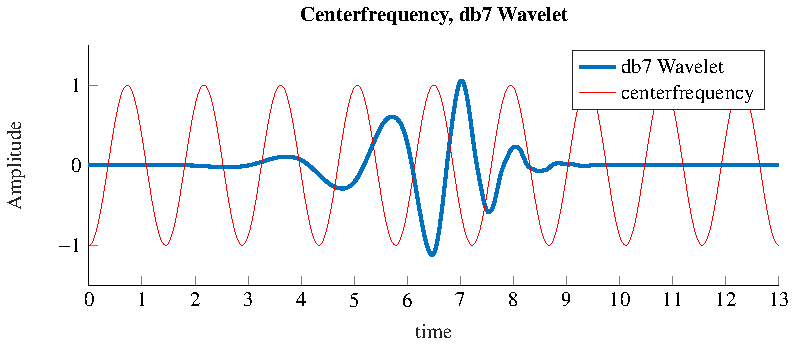
\includegraphics[width=1\textwidth]{papers/wwt/images/centerf.pdf}
	\caption{Approximierte Frequenz eines db7-Wavelet}
	\label{fig:centerf}
\end{figure}

\subsection{Verifikation der approximierten Frequenz}
\label{Freq}
Diese approximierte Frequenz konnte man mit den geeigneten Daten aus der aktuellen Anwendung der Wetterdaten sehr gut verifizieren.
Der Temperaturverlauf während einer Hochdruckphase ist sehr regelmässig und man sollte den 24 Stunden Tagesverlauf exakt erkennen.

Dank der Regelm"assigkeit des Temperaturverlaufs sieht man im \textit{cwt}-Plot eine Erh"ohung des Wertes bei einer gewissen Frequenz.
Die ausgelesene Frequenz beträgt $f = 1.16\cdot10^{-5} \,\text{Hz}$, die umgerechnet einer Periodendauer von $T = 86206.897\,\text{s}\approx 23\,\text{h }56\,\text{min } 47\,\text{s}$ entspricht.
Damit kann die Frequenz im Rückgabewert der Matlab-Funktion als sehr genau bezeichnet werden.
Dabei kommt weiter dazu, dass nur alle f"unf Minuten ein Datenpunkt aufgenommen wurde und somit die Abweichung zu 24 Stunden kleiner ist als die eigentliche Auflösung.

\begin{figure}[h]
	\centering
	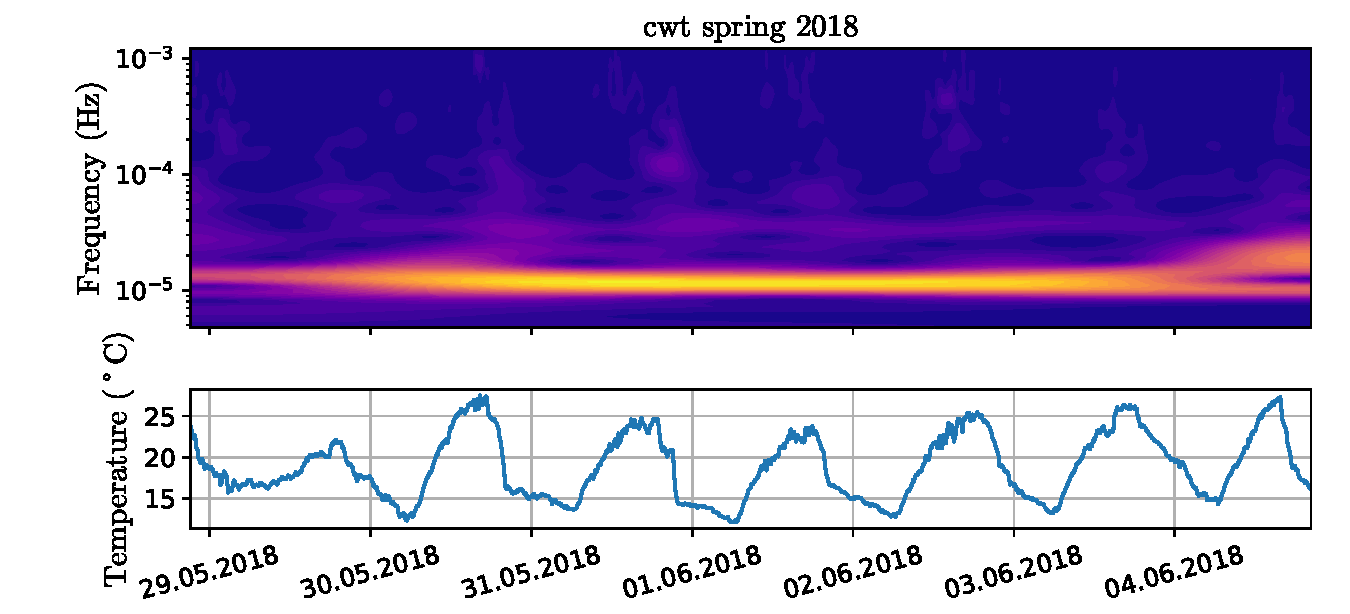
\includegraphics[width=1\textwidth]{papers/wwt/images/data_spring.pdf}
	\caption{Temperaturverlauf und entsprechende cwt}
	\label{fig:cwt_zoom}
\end{figure}



\section{Analyse von Wettereignissen}
\rhead{Analyse von Wetterereignissen}
Aufgrund der Kenntnisse rund um die \textit{cwt} kann angenommen werden, dass ein Wechsel in der Frequenz gut detektiert werden kann.
Bei einer typischen Sturmfront, welche öfters als Wintersturm in den Monaten Dezember und Januar auftreten, zeigten sich bei der Konsultation der Wetterdaten rapide Temperatur- und Luftdruckwechsel sowie ein erhöhtes Windaufkommen.
Das Ziel der Analyse war, solche Ereignisse mittels einer geeigneten \textit{cwt} zu detektieren.
Bei den Rohdaten der Frontdurchgängen erkennt man gemeinsame Wechsel im Wind, der Temperatur sowie dem Luftdruck, daher kann in der Wavelet-Transformation eine erkennbare Antwort erwartet werden. 
Diese korrelierenden auftretenden Frequenzen sollten in der \textit{cwt} sichtbar sein.

\subsection{Parallelen zur Kovarianz}

Um das korrelierende Auftreten der einzelnen Datenkanäle zu verdeutlichen, wurden bei diesen jeweils die zwei zusammengehörenden Koeffizienten der \textit{cwt} miteinander multipliziert. 
Dabei werden die Stellen hervorgehoben, wo beispielsweise der Luftdruck und die Windgeschwindigkeit abhängig voneinander variieren.  
Dies funktioniert besonders gut, da die Werte rasch gegen null gehen falls nur schon einer der beiden Datenverläufe nicht mit dem aktuellen Mutter-Wavelet übereinstimmt.
Genauer betrachtet zeigt dieses Verfahren Ähnlichkeiten mit der Formel
\begin{equation}
COV(X,Y) = \frac{\sum_{i=1}^{N} (x_i- \bar{x})(y_i- \bar{y})}{N-1},
\label{eq:kovarianz}
\end{equation}
der Kovarianz aus der Statistik. Bei dieser Anwendung wird einfach nicht die ganze Zufallsvariable benutzt, sondern nur jeweils die beiden zeitlich übereinstimmenden Werte.

Die Kovarianz zeigt sich nicht nur in dieser Anwendung. Auch schon bei der grundlegenden Formel \ref{eq:cwt1} der \textit{cwt}, kann man gewisse Parallelen sehen. 
In \ref{eq:cwt1} ist die Motivation, die jeweiligen Parameter $a$ und $b$ zu finden, wobei das Mutter-Wavelet und das Signal gemeinsam variieren.
Auch hierfür werden die Produkte der Signale berechnet, auf integriert und gemittelt.
Auch dies ist eine etwas abgewandelte Art der Kovarianz zwischen dem Datensignal und dem Mutter-Wavelet.


Die im Paper angewendete Wavelet-Transformation mit der Idee des Produktes der beiden Datenkanäle,
\begin{equation}
\begin{split}
\mathcal{W}f (a,b)
& =
\biggl<\langle Luftdruck,\psi_{a,b}\rangle, \langle Wind,\psi_{a,b} \rangle \biggr > \\
& = \biggl< \frac{1}{\sqrt{|a|}}\int_{-\infty}^\infty Luftdruck(t)\,\overline{
	\psi\biggl(\frac{t-b}{a}\biggr)}\,dt
,
\frac{1}{\sqrt{|a|}}\int_{-\infty}^\infty Wind(t)\,\overline{
	\psi\biggl(\frac{t-b}{a}\biggr)}\,dt \biggr>
\label{eq:cwt_wwt}
\end{split}
\end{equation}
kann, vorerst nur für den Luftdruck, auf die Kovarianz (Formel \ref{eq:kovarianz}) umgeschrieben werden,

\begin{equation}
COV(Luftdruck, \psi_{a,b})f(a,b) = \frac{\sum_{i=1}^{N} (Luftdruck_i - \overline{Luftdruck})(\psi_{a,b}-  \overline{\psi_{a,b}})}{N-1}.
\end{equation}
Gemäss den Zulässigkeitsbedingungen eines Mutter-Wavelets ist $\overline{\psi_{a,b}} = 0$ (Definition \ref{cwt:zulaessig}). Weiter werden Multiplikationen in Skalarprodukte umgewandelt, somit folgt;
\begin{equation}
COV(Luftdruck, \psi_{a,b})f(a,b) =  \frac{\sum_{i=1}^{N} 
 \langle Luftdruck_i- \overline{Luftdruck},\psi_{a,b}\rangle}{N-1}.
\end{equation}
Weiter Ausmultipliziert
\begin{equation}
COV(Luftdruck, \psi_{a,b})f(a,b) = \frac{\sum_{i=1}^{N} 
\langle Luftdruck_i,\psi_{a,b}\rangle - \langle \overline{Luftdruck},\psi_{a,b}\rangle}{N-1},
\end{equation}
schlussendlich ergibt sich mit $\langle \overline{Luftdruck},\psi_{a,b} \rangle = 0$,
\begin{equation}
COV(Luftdruck, \psi_{a,b})f(a,b) = \frac{\sum_{i=1}^{N} 
	\langle Luftdruck_i,\psi_{a,b}\rangle}{N-1}.
\end{equation}
 Wird noch das Produkt mit dem Wind hinzugenommen
 \begin{equation}
 \begin{split}
\biggl< COV(Luftdruck, \psi_{a,b})f(a,b), COV(Wind), \psi_{a,b})f(a,b) \biggr > \\
=
 \biggl< \frac{\sum_{i=1}^{N} 
 	\langle Luftdruck_i,\psi_{a,b}\rangle}{N-1},\frac{\sum_{i=1}^{N} 
 	\langle Wind_i,\psi_{a,b}\rangle}{N-1} \biggr >,
 \label{eq:cov_wwt}
 \end{split}
 \end{equation}
 wurde die Herleitung von der Wavelet-Transformation in der Formel \ref{eq:cwt_wwt} zum einem äquivalenten Resultat, ohne die Korrekturfaktoren, mit der Kovarianz in der Formel \ref{eq:cov_wwt} gezeigt.



\subsection{Sturmsaison 2018}
\rhead{Sturmsaison 2018}
Bereits bekannt war, dass in der Sturmsaison im Jahre 2018 einige heftige Winterstürme aufgetreten sind.
So wurde bei der Analyse der Daten nur auf diese Periode das Augenmerk gelegt. 
In Abbildung \ref{fig:cwt_storm} \space sieht man die Wavelet-Transformation des Luftdruckes und Windes miteinander multipliziert.
Dies über die Monate Januar und Februar im Jahre 2018 hinweg.
Weiter wird der Luftdruck- und Windverlauf dargestellt.
 
\begin{figure}[h]
	\centering
	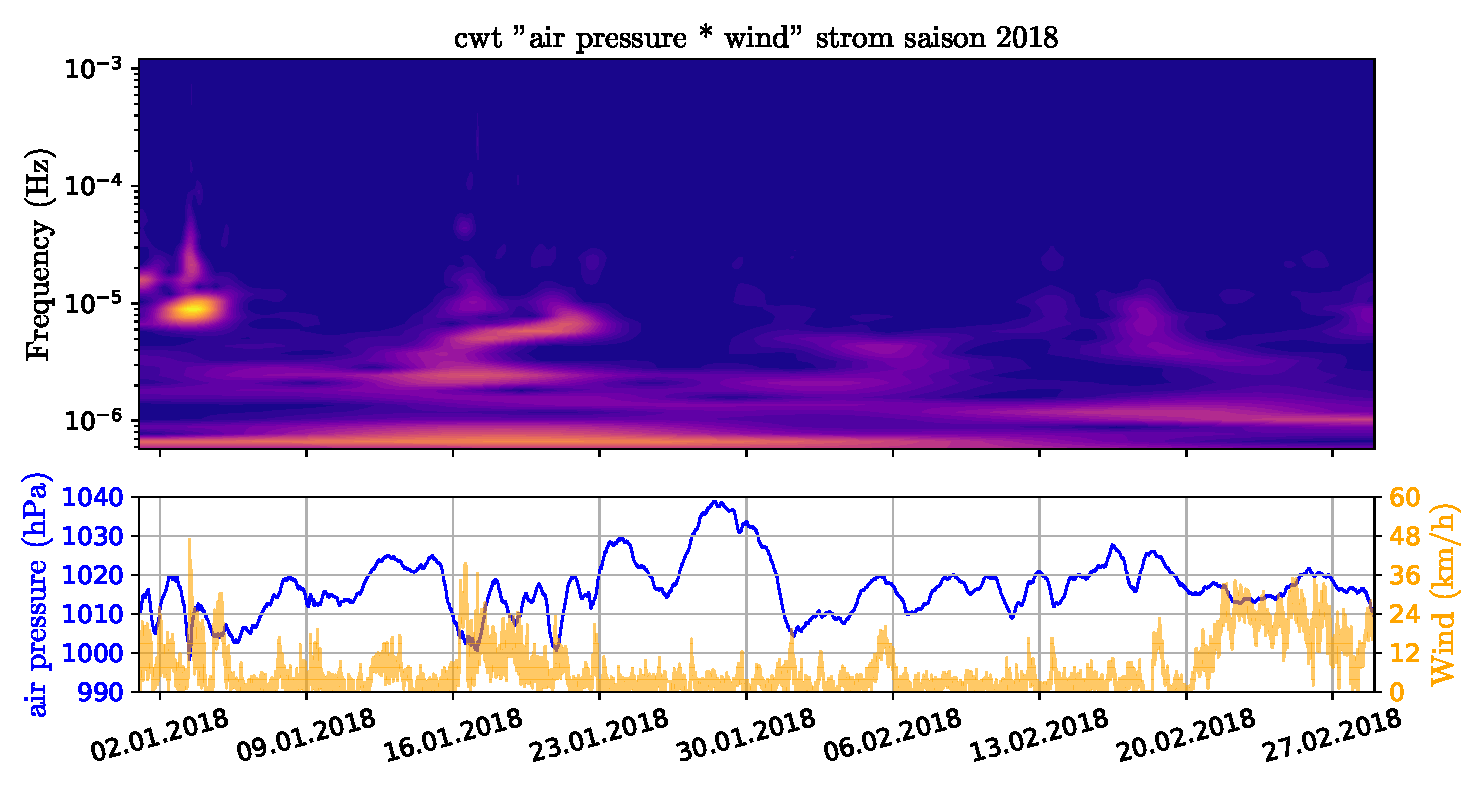
\includegraphics[width=1\textwidth]{papers/wwt/images/storm_airp_wind.pdf}
	\caption{Cwt und Rohdaten Sturmsaison 2018}
	\label{fig:cwt_storm}
\end{figure}

In Abbildung \ref{fig:cwt_storm} \space zeigen sich um den 3. sowie zwischen dem 16. und 23. Januar jeweils gewisse Frequenzen des Windes und des Luftdruckes, die gemeinsam auf die Wavelet-Transformation angesprochen haben.

\subsubsection{Wintersturm {\em Burglind} }
\label{burglind}
Hineingezoomt um den 3. Januar (Abbildung \ref{fig:cwt_storm_zoom}) sind im Rohdatenverlauf die Aktivitäten des Windes und Luftdruckes erkennbar. 
\begin{figure}[b]
	\centering
	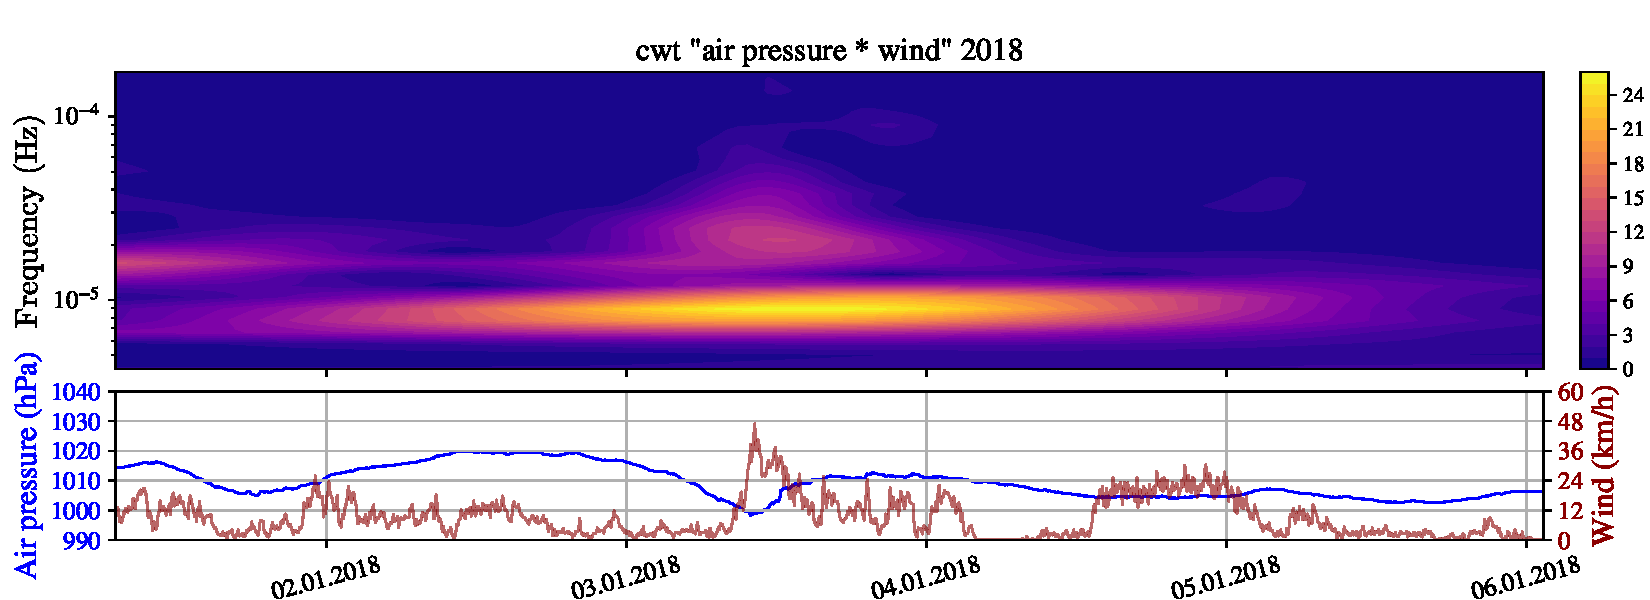
\includegraphics[width=1\textwidth]{papers/wwt/images/storm_airp_wind_zoom.pdf}
	\caption{Cwt und Rohdaten Wintersturm {\em Burglind}  2018}
	\label{fig:cwt_storm_zoom}
\end{figure}
Aus dem Fachbericht \space \cite{Fachbericht:Burglind} von Meteoschweiz war bekannt, dass am Vormittag des 3. Januars 2018 die stärkste Sturmfront seit dem verheerenden Sturm Lothar aus dem Jahre 1999 über die Schweiz zog.
Dabei zeigt sich eindrücklich, wie der Sturmdurchgang in der multiplizierten Wavelet-Transformation hervorgehoben wird.

\subsubsection{Sturmtief {\em Evi}  und {\em Friedricke} }
\label{evi}
Beim zweiten Ereignis zwischen dem 16. und 23. Januar trat die Aktivität nicht mehr so deutlich auf.
Nach dem Sturmarchiv  \cite{online:sturmarchiv} traf am 16. Januar das Sturmtief {\em Evi}  und am 18. Januar das Sturmtief {\em Friedricke} auf Europa. Dabei zeigt sich nach der Amplitude, dass das Sturmtief nicht direkt auf die Schweiz traf, sonder diese lediglich streifte. 

\begin{figure}[h]
	\centering
	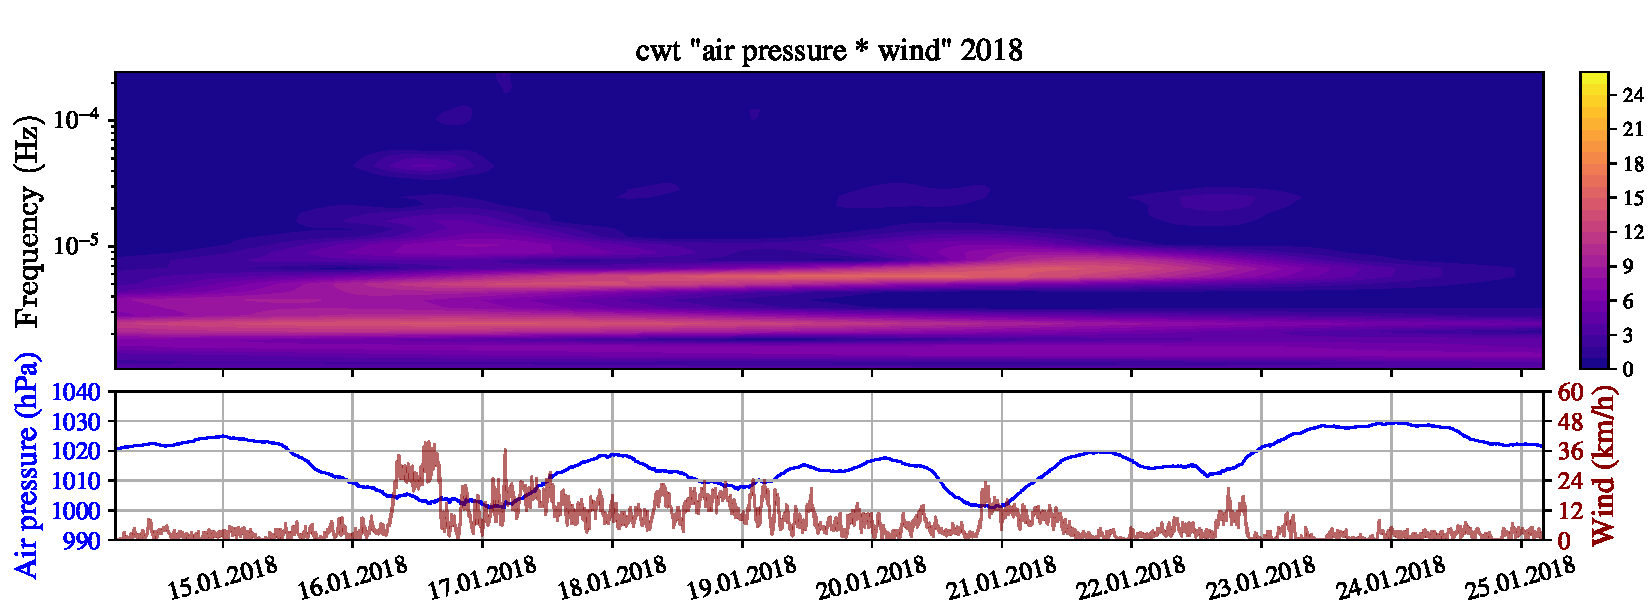
\includegraphics[width=1\textwidth]{papers/wwt/images/storm_airp_wind_zoom2.pdf}
	\caption{Cwt und Rohdaten Strumtief {\em Evi}  und {\em Friedricke} 2018}
	\label{fig:cwt_storm_zoom2}
\end{figure}



\section{Schlussfolgerung}
\rhead{Schlussfolgerung}

Mit dem Versuch, die Wavelet-Transformation im Bereich der Wetteranalyse nützlich anzuwenden, zeigt sich, dass dies durchaus möglich ist.
In der Anwendung mit dem Phänomen der Winterstürme wurde die Wavelet-Transformation oder genauer die stetige Wavelet-Transformation erfolgreich eingesetzt.
Es können zwei Hypothesen aufgestellt werden:
\begin{itemize}
	\item Die periodischen Tagesverläufe bei konstanten Wetterverhältnissen führen dazu, dass die Wavelet-Koeffizienten der \textit{cwt} bei dieser Frequenz deutlich ansteigen (\ref{Freq}).
	
	\item Nicht periodische Ereignisse äussern sich durch das korrelierte Auftreten bei der Betrachtung mehrerer Datenkanäle. Dies kann mit dem Produkt der Wavelet-Koeffizienten oder eben der Kovarianz analysiert werden (\ref{burglind}).
\end{itemize}


Damit ist selbstverständlich noch nichts abschliessend bewiesen. Die Hypothesen müssten detaillierter analysiert werden.
Auch sollte die Methode weiterführend auf andere meteorologische Ereignisse angewandt werden.
Zum Beispiel könnte man versuchen, Gewitter zu detektieren.
Falls sich diese Methode für mehrere Phänomene beweisen lässt, ist eine praktische Anwendung möglich und durchaus vorstellbar. 

\section{Anhang}
Anbei in Abbildung \ref{fig:python-plot-code} und \ref{fig:python-plot-code2} der verwendete Code zum Plotten der Abbildung \ref{fig:cwt_storm}.

\begin{figure}[h]
	\centering
	\lstinputlisting[language=Python,firstline = 1, lastline = 39, numbers=left, firstnumber=1, style = Python]{papers/wwt/code/plot_burglind.py}
	\caption{Python Codeausschnitt}
	\label{fig:python-plot-code}
\end{figure}
\begin{figure}[h]
	\centering
	\lstinputlisting[language=Python,firstline = 40, lastline = 91, firstnumber=40, numbers=left,style = Python]{papers/wwt/code/plot_burglind.py}
	\caption{Python Codeausschnitt}
	\label{fig:python-plot-code2}
\end{figure}
 
 \newpage

\printbibliography[heading=subbibliography]
\end{refsection}

%
% main.tex -- Paper zum Thema wwt
%
% (c) 2019 Michael Schmid, Hochschule Rapperswil
%
\chapter{Wetter-Wavelet-Transformation\label{chapter:wwt}}
\lhead{Wetter-Wavelet-Transformation}
\begin{refsection}
\chapterauthor{Michael Schmid}



\definecolor{codegreen}{rgb}{0,0.6,0}
\definecolor{codegray}{rgb}{0.5,0.5,0.5}
\definecolor{codepurple}{rgb}{0.58,0,0.82}
\definecolor{backcolour}{rgb}{0.95,0.95,0.92}

\lstdefinestyle{mystyle}{
	backgroundcolor=\color{backcolour},   
	commentstyle=\color{codegreen},
	keywordstyle=\color{magenta},
	numberstyle=\tiny\color{codegray},
	stringstyle=\color{codepurple},
	basicstyle=\footnotesize,
	breakatwhitespace=false,         
	breaklines=true,                 
	captionpos=b,                    
	keepspaces=true,                 
	numbers=left,                    
	numbersep=2pt,                  
	showspaces=false,                
	showstringspaces=false,
	showtabs=false,                  
	tabsize=2
}
\lstset{style=mystyle}
\lstdefinestyle{mystyle}{
	morekeywords={cwt,contourf,datetick}
}


\section{Einführung}
\rhead{Einführung}


Seit Langem konsultiere ich meine aktuellen Wetterdaten über eine eher unübliche Internetseite.
Dabei handelt es sich um eine privat geführte Wetterstation, welche die gemessenen Daten im Internet grafisch darstellt.
Die Daten werden auch tabellarisch zur Verfügung gestellt.
Das Feature, welches ich bis anhin am regelmässigsten nutzte, war die grafische Darstellung der aktuellen Wetterdaten über den Zeitraum der letzten 24 Stunden.
Bei speziellen Ereignissen im Wetterverlauf fielen mir besondere und wiederkehrende Charakteristiken auf.
\\

Nach der Einführung in die Theorie der Wavelets kam mir die Idee, solche Wetterphänomene mit einer geeigneten Wavelet Transformation zu detektieren.
In diesem Paper wird einerseits auf die theoretischen Grundlagen der angewandten Methoden zurückgegriffen sowie die besprochenen meteorologischen Phänomene kurz erläutert. 
Weiterführend wird auf die verwendeten Methoden, auch in der praktischen Anwendung, vertieft eingegangen.
Ein besonderes Augenmerk wird auf die allgemeine Vorgehensweise sowie deren Schwierigkeiten gelegt.
\\




\section{Wetterstation Seegräben}
\rhead{Wetterstation Seegräben}

Die angesprochene Wetterstation in der Gemeinde Seegräben im Kanton Zürich ist mit einer DAVIS Vantage Pro2 6153 \cite{online:davisinstruments} realisiert worden.
Sie verfügt über Sensoren für die Temperatur, Feuchtigkeit, Geschwindigkeit und Richtung des Windes sowie für den Niederschlag. 
Durch diese Sensoren werden folgende Daten aufgezeichnet:


\begin{itemize}
	\item \textbf{Aussentemperatur} in Grad Celsius
	\item \textbf{Relative Luftfeuchtigkeit} in Prozent
	\item \textbf{Luftdruck} in hPa
	\item \textbf{Windgeschwindigkeit} in km/h, gemittelt über 5 Minuten
	\item \textbf{Windböen} in km/h
	\item \textbf{Windrichtung} nach Himmelsrichtung
	\item \textbf{Regenmenge} in $\text{l/m}^{2}$
\end{itemize}	


Der Thermo- / Feuchtigkeitssensor liegt zusammen mit dem Regenmengenmesser auf 2 Meter über Boden.
Mit einem Abstand von rund 10 Meter zum nächsten Gebäude sind optimale Messbedingungen geschaffen.
Mit einem Mast ist der Windmesser auf 1.5 Meter über dem First eines Gebäudes lokalisiert \space \cite{online:wss}.
Die Daten werden anschliessend mit einer Software von PC-Wetterstation.de weiterverarbeitet und auf der Website \cite{online:wss} veröffentlicht.
Mehr zur Verwendung der Wetterdaten im n\"achsten Abschnitt.

\section{Datenaufarbeitung}
\rhead{Datenaufarbeitung}
Der n\"achste Vorbereitungsschritt zur Wavelet Transformation war die Aufbereitung der zur Verf\"ugung gestellten Daten der Wetterstation. Dazu musste erst analysiert werden, wie die Daten auf der Website dargestellt werden.
\subsection{Wetter-Archiv}
Auf der Website gibt es mehrere Möglichkeiten, sich Wetterdaten aus der Vergangenheit darstellen zu lassen.
In der Kategorie des Archivs auf der Website kann man die Wetterdaten eines gew\"unschten Zeitraums tabellarisch oder grafisch darstellen lassen.
Vom Betreiber der Website steht keine Funktion zur Verfügung, welche es erlaubt, die Daten offiziell und automatisch herunterzuladen.
\subsection{Datenerfassung}
Da f\"ur die angestrebte Anwendung eine m\"oglichst hohe Aufl\"osung der jeweiligen Daten erforderlich ist, mussten die Daten im Zeitraum von einem Tag dargestellt werden.
Dies hatte zur Folge, dass man f\"ur jeden Tag eine Tabelle auf dem Archiv der Website \"offnen musste. Man hätte anschliessend die Daten mit copy and paste in eine Excel-Tabelle einf\"ugen können. Daher wurde  entschieden, ein Programm zu schreiben, welches diese Aufgabe automatisieren sollte.
Als Programmiersprache wurde hierf\"ur Python gewählt.


Mit der Pandas Library und der Funktion \texttt{'read\_html'} \space konnten die Daten direkt aus dem Python Programm von der Website heruntergeladen werden.
Entscheidend für das Gelingen dieser Teilaufgabe war, dass die URL-Links der einzelnen Tage stets regelmässig aufgebaut sind:
\\
\\
$$\centering{\textit{https://www.wetter-seegraeben.ch/uploads/insert.php?insert=\textbf{20190701}.htm}}$$
\\
Wie zu sehen ist, wird der Link mit dem Datum regelmässig aufgebaut. Somit konnten die entsprechenden Links mit mehreren While-Schleife zusammengesetzt werden.
In der Abbildung \ref{fig:python-code} ist der wesentliche Ausschnitt aus dem Python Code dargestellt.
\begin{figure}
	\centering
	\lstinputlisting[language=Python,firstline=1,lastline=16,numbers=left,style = Python]{papers/wwt/code/get_data.py}
	\caption{Python Codeausschnitt}
	\label{fig:python-code}
\end{figure}
Die Daten konnten im nächsten Schritt in einer Excel-Tabelle abgespeichert werden.
Dort folgte der letzte Feinschliff; d.h. alle überflüssigen Kopfzeilen und Statistiken wurden entfernt.

\subsubsection{Unregelmässigkeiten der Wetterstation}
Bei der Datenerfassung durch das eben beschriebene Python Programm wurden einige Unregelmässigkeiten der Wetterstation beobachtet.
Das Programm wird jeweils durch eine Fehlermeldung abgebrochen, wenn der angegebene Link nicht abrufbar ist. 
So fiel auf, dass unregelmässig auf das Jahr verteilt, Daten von gewissen Tagen fehlten. Es stellte sich heraus, dass hinter dem eigentlich korrektem Link die entsprechende Internetseite nicht zur Verfügung steht.
Wird manuell auf der Website nach diesem Tag gesucht, kann nichts gefunden werden.
Dies trat teilweise sogar in Abschnitten von mehreren Tagen auf.
Wie sich später herausstellte, traten die fehlenden Tagen nicht zu den Zeitpunkten auf, die mich interessierten.


\subsection{Datendarstellung}
Die Darstellung der gewonnenen Daten konnte einfach mittels Python realisiert werden.
Anbei in Abbildung \ref{fig:rawdata} der Plot der Rohdaten aus dem Jahre 2018, wobei nur jeder zehnte Messpunkt verwendet wurde.
Diese Rohdaten dienten als Grundlage für alle weiteren Berechnungen. 
\begin{figure}
	\centering
	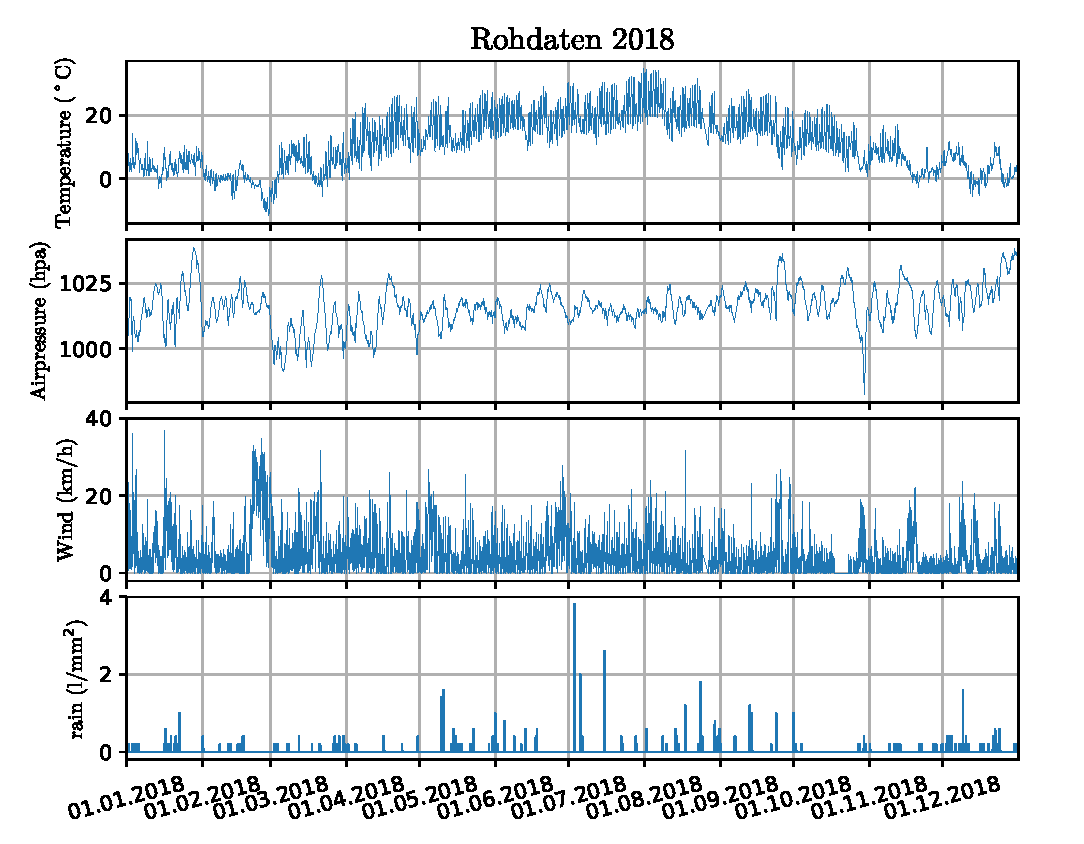
\includegraphics[width=1\textwidth]{papers/wwt/images/raw.pdf}
	\caption{Rohdaten 2018}
	\label{fig:rawdata}
\end{figure}


\section{Stetige Wavelet-Transformation}
\rhead{Stetige Wavelet-Transformation}
Die theoretischen Grundlagen rund um die stetige Wavelet-Transformation wurden im Kapitel \ref{chapter:cwt} genaustens erläutert. 
In diesem Abschnitt der Seminararbeit wird öfters auf die Theorie des angesprochenen Kapitels \ref{chapter:cwt} referenziert ohne diese genauer zu erläutern. 

Für eine m"oglichst aussagekräftige Untersuchung der Signale, in welcher so viele Informationen gewonnen werden sollten wie m"oglich, eignet sich die stetige Wavelet-Transformation (folgend noch kurz \textit{cwt} aus dem Englischen "continuous wavelet transform"). 
Regelmässig auftretende Frequenzen können dank der \textit{cwt} gefunden und zusätzlich einem Zeitraum zugeordnet werden.
\subsection{Das verwendete Wavelet}
In
\begin{equation}
\mathcal{W}f (a,b)
=
\langle f,\psi_{a,b}\rangle
=
\frac{1}{\sqrt{|a|}}\int_{-\infty}^\infty f(t)\,\overline{
	\psi\biggl(\frac{t-b}{a}\biggr)}\,dt
\label{eq:cwt1}
\end{equation}
erkennt man die grundlegende Formel der \textit{cwt}.
Wobei das $\psi_{a,b}$ für das Mutter-Wavelet steht, welches mit dem Koeffizienten $a$ skaliert und mit $b$ verschoben wird.

Als Mutter-Wavelet wurde 
\begin{equation}
\psi_{Gabor}(t) =  c_{\sigma} e^{-\frac{1}{2}t^2} \biggl(e^{i \sigma t}- e^{-\frac{1}{2} \sigma^2} \biggr)
\label{eq:morlet}
\end{equation} \cite{online:Morlet}
verwendet, welches auch als das analytische Gabor-Wavelet bekannt ist.
Dabei gibt $\sigma$ an, wie hoch die Frequenz ist und dementsprechend auch, wie viele lokale Maxima und Minima innerhalb des Gauss'schen Fensters das Mutter-Wavelet existieren.
Weiter ist $c_{\sigma}$ eine reelle Konstante und dient zur Erf"ullung der Zulässigkeitsbedingungen in der Definition \ref{cwt:zulaessig}.
Das Morlet-Wavelet wird in der Abbildung \ref{fig:gabor_plot} \space dargestellt und $\sigma$ wurde auf 5 gesetzt.

\begin{figure}
\centering
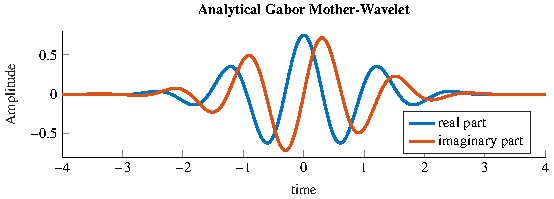
\includegraphics[width=1\textwidth]{papers/wwt/images/gabor.pdf}
\caption{Analytisches Gabor Mutter-Wavelet}
\label{fig:gabor_plot}
\end{figure}

Weiter ist zu erwähnen, dass das eben gezeigte Gabor Wavelet der referenzierten Quelle entnommen wurde. Ob Matlab die selbe Form verwendet, konnte nicht abschliessend geklärt werden.

\subsection{Berechung mit Matlab}
Die Berechnung der \textit{cwt} wurde mit der numerischen Berechnungs-Software Matlab durchgeführt.
Die dafür verwendete Funktion war die cwt()-Funktion.
Die Funktion arbeitete bei korrekter Parametrisierung wie gewünscht.
Falls man verstehen möchte wie die Funktion genau rechnet, muss man sich mit einer eher dürftigen Dokumentation herumschlagen.
Folgende Parameter wurden verwendet
\lstinputlisting[language=Matlab,firstline=1,lastline=1,  numbers=left, style = mystyle]{papers/wwt/code/matlab.m}
\label{fig:matlab_code_cwt}
wobei Matlab das Gabor-Wavelet als \texttt{'amor'} bezeichnet, mit \texttt{'VoicesPerOctave'} konnte die Genauigkeit erhöht werden und die Variable \texttt{'fs'} beschreibt die Abtastfrequenz der Messsignale.
Bei den Rückgabewerten werden die Wavelet-Werte in \texttt{'wt'} als komplexe Matrix und die approximierten Frequenzen in \texttt{'F'} abgespeichert.

Anstelle des Skalierungsfaktors $a$ in der Gleichung \ref{eq:cwt} berechnet Matlab eine approximierte Frequenz und gibt diese zurück.
Für jeden verwendeten Skalierungsfaktor $a$ wird eine Sinuskurve gesucht, die am ehesten mit der Frequenz des entsprechenden Wavelets übereinstimmt.
Siehe das Beispiel mit einem Daubechies Wavelet der Nummer 7 in der Abbildung \ref{fig:centerf}.
Dies dient dazu den Wavelet-Koeffizienten einer Frequenz zuzuordnen. 
Aus dem verwendeten Skalierungsfaktor $a$ könnte auf die Schnelle keine Information entnommen werden.
\begin{figure}[h]
	\centering
	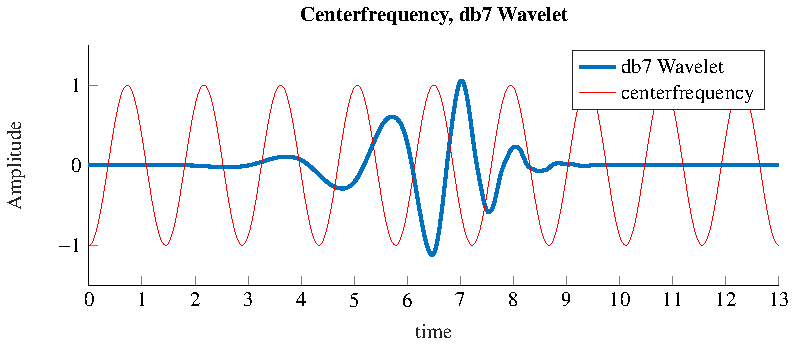
\includegraphics[width=1\textwidth]{papers/wwt/images/centerf.pdf}
	\caption{Approximierte Frequenz eines db7-Wavelet}
	\label{fig:centerf}
\end{figure}

\subsection{Verifikation der approximierten Frequenz}
\label{Freq}
Diese approximierte Frequenz konnte man mit den geeigneten Daten aus der aktuellen Anwendung der Wetterdaten sehr gut verifizieren.
Der Temperaturverlauf während einer Hochdruckphase ist sehr regelmässig und man sollte den 24 Stunden Tagesverlauf exakt erkennen.

Dank der Regelm"assigkeit des Temperaturverlaufs sieht man im \textit{cwt}-Plot eine Erh"ohung des Wertes bei einer gewissen Frequenz.
Die ausgelesene Frequenz beträgt $f = 1.16\cdot10^{-5} \,\text{Hz}$, die umgerechnet einer Periodendauer von $T = 86206.897\,\text{s}\approx 23\,\text{h }56\,\text{min } 47\,\text{s}$ entspricht.
Damit kann die Frequenz im Rückgabewert der Matlab-Funktion als sehr genau bezeichnet werden.
Dabei kommt weiter dazu, dass nur alle f"unf Minuten ein Datenpunkt aufgenommen wurde und somit die Abweichung zu 24 Stunden kleiner ist als die eigentliche Auflösung.

\begin{figure}[h]
	\centering
	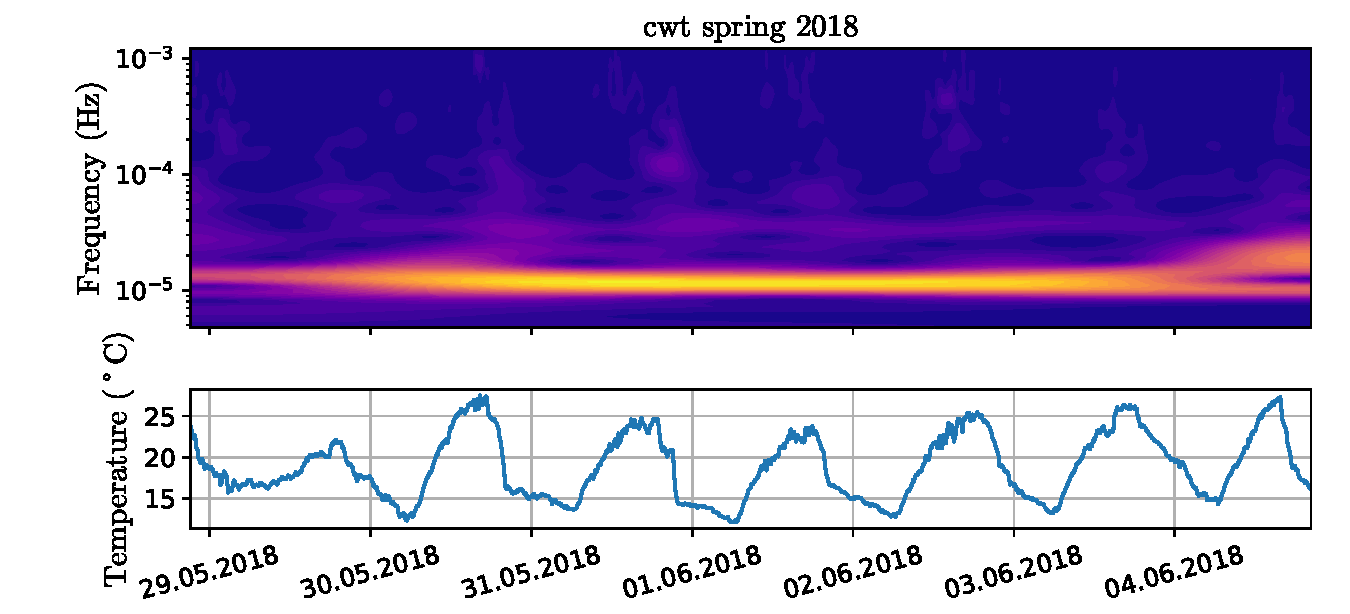
\includegraphics[width=1\textwidth]{papers/wwt/images/data_spring.pdf}
	\caption{Temperaturverlauf und entsprechende cwt}
	\label{fig:cwt_zoom}
\end{figure}



\section{Analyse von Wettereignissen}
\rhead{Analyse von Wetterereignissen}
Aufgrund der Kenntnisse rund um die \textit{cwt} kann angenommen werden, dass ein Wechsel in der Frequenz gut detektiert werden kann.
Bei einer typischen Sturmfront, welche öfters als Wintersturm in den Monaten Dezember und Januar auftreten, zeigten sich bei der Konsultation der Wetterdaten rapide Temperatur- und Luftdruckwechsel sowie ein erhöhtes Windaufkommen.
Das Ziel der Analyse war, solche Ereignisse mittels einer geeigneten \textit{cwt} zu detektieren.
Bei den Rohdaten der Frontdurchgängen erkennt man gemeinsame Wechsel im Wind, der Temperatur sowie dem Luftdruck, daher kann in der Wavelet-Transformation eine erkennbare Antwort erwartet werden. 
Diese korrelierenden auftretenden Frequenzen sollten in der \textit{cwt} sichtbar sein.

\subsection{Parallelen zur Kovarianz}

Um das korrelierende Auftreten der einzelnen Datenkanäle zu verdeutlichen, wurden bei diesen jeweils die zwei zusammengehörenden Koeffizienten der \textit{cwt} miteinander multipliziert. 
Dabei werden die Stellen hervorgehoben, wo beispielsweise der Luftdruck und die Windgeschwindigkeit abhängig voneinander variieren.  
Dies funktioniert besonders gut, da die Werte rasch gegen null gehen falls nur schon einer der beiden Datenverläufe nicht mit dem aktuellen Mutter-Wavelet übereinstimmt.
Genauer betrachtet zeigt dieses Verfahren Ähnlichkeiten mit der Formel
\begin{equation}
COV(X,Y) = \frac{\sum_{i=1}^{N} (x_i- \bar{x})(y_i- \bar{y})}{N-1},
\label{eq:kovarianz}
\end{equation}
der Kovarianz aus der Statistik. Bei dieser Anwendung wird einfach nicht die ganze Zufallsvariable benutzt, sondern nur jeweils die beiden zeitlich übereinstimmenden Werte.

Die Kovarianz zeigt sich nicht nur in dieser Anwendung. Auch schon bei der grundlegenden Formel \ref{eq:cwt1} der \textit{cwt}, kann man gewisse Parallelen sehen. 
In \ref{eq:cwt1} ist die Motivation, die jeweiligen Parameter $a$ und $b$ zu finden, wobei das Mutter-Wavelet und das Signal gemeinsam variieren.
Auch hierfür werden die Produkte der Signale berechnet, auf integriert und gemittelt.
Auch dies ist eine etwas abgewandelte Art der Kovarianz zwischen dem Datensignal und dem Mutter-Wavelet.


Die im Paper angewendete Wavelet-Transformation mit der Idee des Produktes der beiden Datenkanäle,
\begin{equation}
\begin{split}
\mathcal{W}f (a,b)
& =
\biggl<\langle Luftdruck,\psi_{a,b}\rangle, \langle Wind,\psi_{a,b} \rangle \biggr > \\
& = \biggl< \frac{1}{\sqrt{|a|}}\int_{-\infty}^\infty Luftdruck(t)\,\overline{
	\psi\biggl(\frac{t-b}{a}\biggr)}\,dt
,
\frac{1}{\sqrt{|a|}}\int_{-\infty}^\infty Wind(t)\,\overline{
	\psi\biggl(\frac{t-b}{a}\biggr)}\,dt \biggr>
\label{eq:cwt_wwt}
\end{split}
\end{equation}
kann, vorerst nur für den Luftdruck, auf die Kovarianz (Formel \ref{eq:kovarianz}) umgeschrieben werden,

\begin{equation}
COV(Luftdruck, \psi_{a,b})f(a,b) = \frac{\sum_{i=1}^{N} (Luftdruck_i - \overline{Luftdruck})(\psi_{a,b}-  \overline{\psi_{a,b}})}{N-1}.
\end{equation}
Gemäss den Zulässigkeitsbedingungen eines Mutter-Wavelets ist $\overline{\psi_{a,b}} = 0$ (Definition \ref{cwt:zulaessig}). Weiter werden Multiplikationen in Skalarprodukte umgewandelt, somit folgt;
\begin{equation}
COV(Luftdruck, \psi_{a,b})f(a,b) =  \frac{\sum_{i=1}^{N} 
 \langle Luftdruck_i- \overline{Luftdruck},\psi_{a,b}\rangle}{N-1}.
\end{equation}
Weiter Ausmultipliziert
\begin{equation}
COV(Luftdruck, \psi_{a,b})f(a,b) = \frac{\sum_{i=1}^{N} 
\langle Luftdruck_i,\psi_{a,b}\rangle - \langle \overline{Luftdruck},\psi_{a,b}\rangle}{N-1},
\end{equation}
schlussendlich ergibt sich mit $\langle \overline{Luftdruck},\psi_{a,b} \rangle = 0$,
\begin{equation}
COV(Luftdruck, \psi_{a,b})f(a,b) = \frac{\sum_{i=1}^{N} 
	\langle Luftdruck_i,\psi_{a,b}\rangle}{N-1}.
\end{equation}
 Wird noch das Produkt mit dem Wind hinzugenommen
 \begin{equation}
 \begin{split}
\biggl< COV(Luftdruck, \psi_{a,b})f(a,b), COV(Wind), \psi_{a,b})f(a,b) \biggr > \\
=
 \biggl< \frac{\sum_{i=1}^{N} 
 	\langle Luftdruck_i,\psi_{a,b}\rangle}{N-1},\frac{\sum_{i=1}^{N} 
 	\langle Wind_i,\psi_{a,b}\rangle}{N-1} \biggr >,
 \label{eq:cov_wwt}
 \end{split}
 \end{equation}
 wurde die Herleitung von der Wavelet-Transformation in der Formel \ref{eq:cwt_wwt} zum einem äquivalenten Resultat, ohne die Korrekturfaktoren, mit der Kovarianz in der Formel \ref{eq:cov_wwt} gezeigt.



\subsection{Sturmsaison 2018}
\rhead{Sturmsaison 2018}
Bereits bekannt war, dass in der Sturmsaison im Jahre 2018 einige heftige Winterstürme aufgetreten sind.
So wurde bei der Analyse der Daten nur auf diese Periode das Augenmerk gelegt. 
In Abbildung \ref{fig:cwt_storm} \space sieht man die Wavelet-Transformation des Luftdruckes und Windes miteinander multipliziert.
Dies über die Monate Januar und Februar im Jahre 2018 hinweg.
Weiter wird der Luftdruck- und Windverlauf dargestellt.
 
\begin{figure}[h]
	\centering
	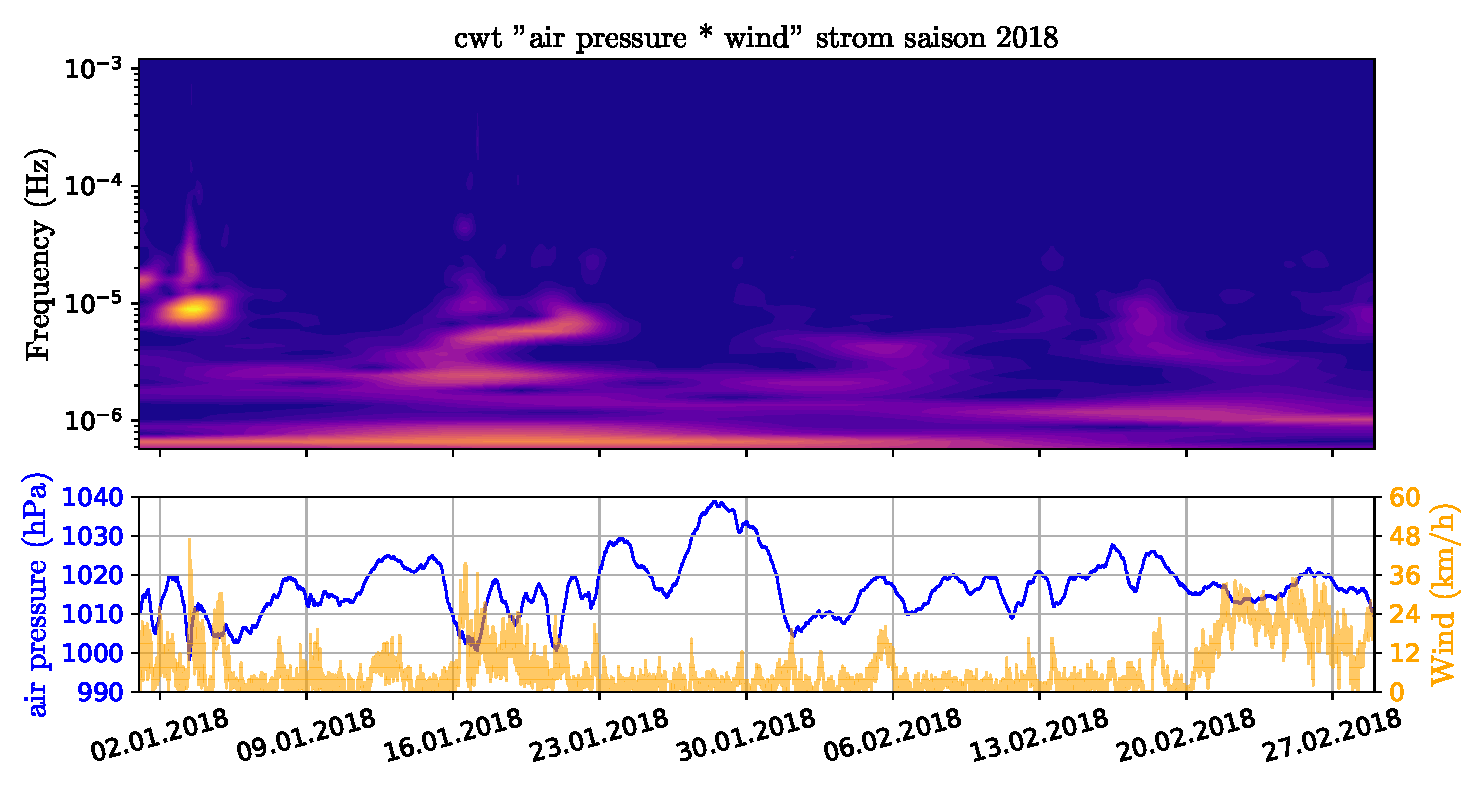
\includegraphics[width=1\textwidth]{papers/wwt/images/storm_airp_wind.pdf}
	\caption{Cwt und Rohdaten Sturmsaison 2018}
	\label{fig:cwt_storm}
\end{figure}

In Abbildung \ref{fig:cwt_storm} \space zeigen sich um den 3. sowie zwischen dem 16. und 23. Januar jeweils gewisse Frequenzen des Windes und des Luftdruckes, die gemeinsam auf die Wavelet-Transformation angesprochen haben.

\subsubsection{Wintersturm {\em Burglind} }
\label{burglind}
Hineingezoomt um den 3. Januar (Abbildung \ref{fig:cwt_storm_zoom}) sind im Rohdatenverlauf die Aktivitäten des Windes und Luftdruckes erkennbar. 
\begin{figure}[b]
	\centering
	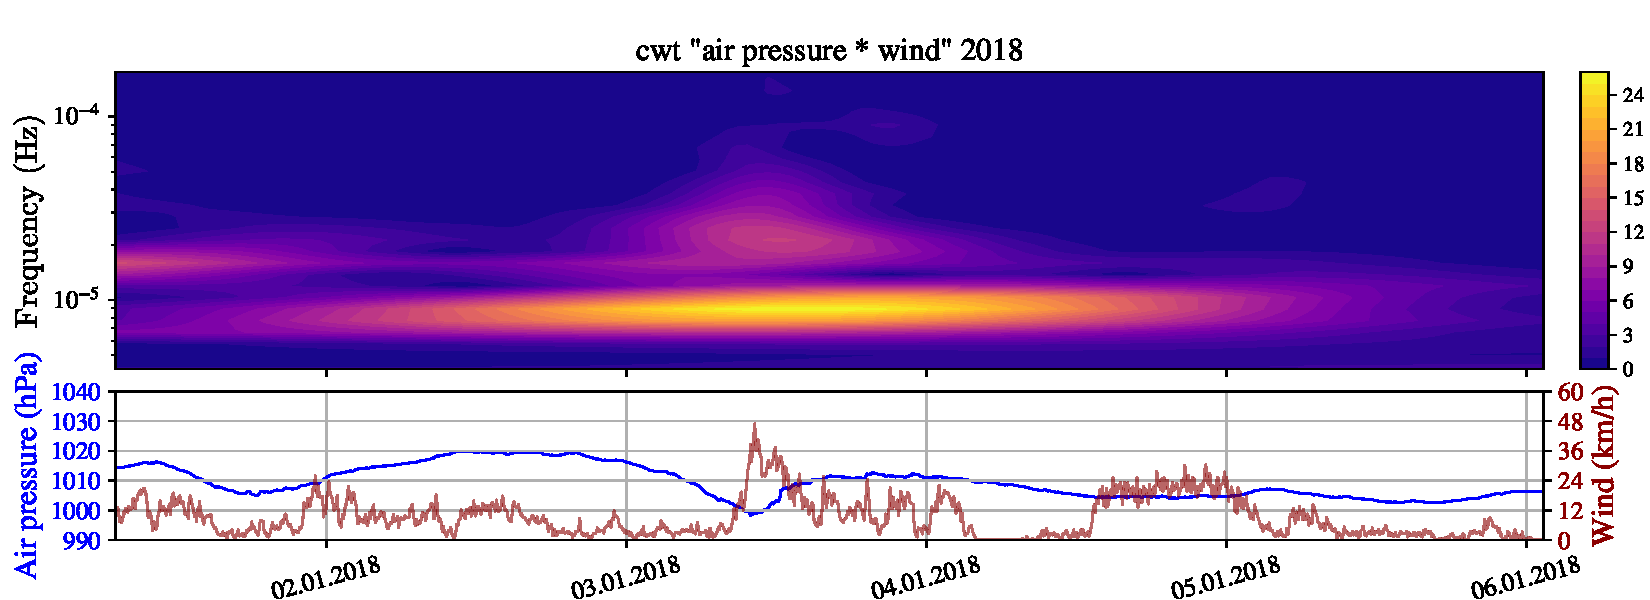
\includegraphics[width=1\textwidth]{papers/wwt/images/storm_airp_wind_zoom.pdf}
	\caption{Cwt und Rohdaten Wintersturm {\em Burglind}  2018}
	\label{fig:cwt_storm_zoom}
\end{figure}
Aus dem Fachbericht \space \cite{Fachbericht:Burglind} von Meteoschweiz war bekannt, dass am Vormittag des 3. Januars 2018 die stärkste Sturmfront seit dem verheerenden Sturm Lothar aus dem Jahre 1999 über die Schweiz zog.
Dabei zeigt sich eindrücklich, wie der Sturmdurchgang in der multiplizierten Wavelet-Transformation hervorgehoben wird.

\subsubsection{Sturmtief {\em Evi}  und {\em Friedricke} }
\label{evi}
Beim zweiten Ereignis zwischen dem 16. und 23. Januar trat die Aktivität nicht mehr so deutlich auf.
Nach dem Sturmarchiv  \cite{online:sturmarchiv} traf am 16. Januar das Sturmtief {\em Evi}  und am 18. Januar das Sturmtief {\em Friedricke} auf Europa. Dabei zeigt sich nach der Amplitude, dass das Sturmtief nicht direkt auf die Schweiz traf, sonder diese lediglich streifte. 

\begin{figure}[h]
	\centering
	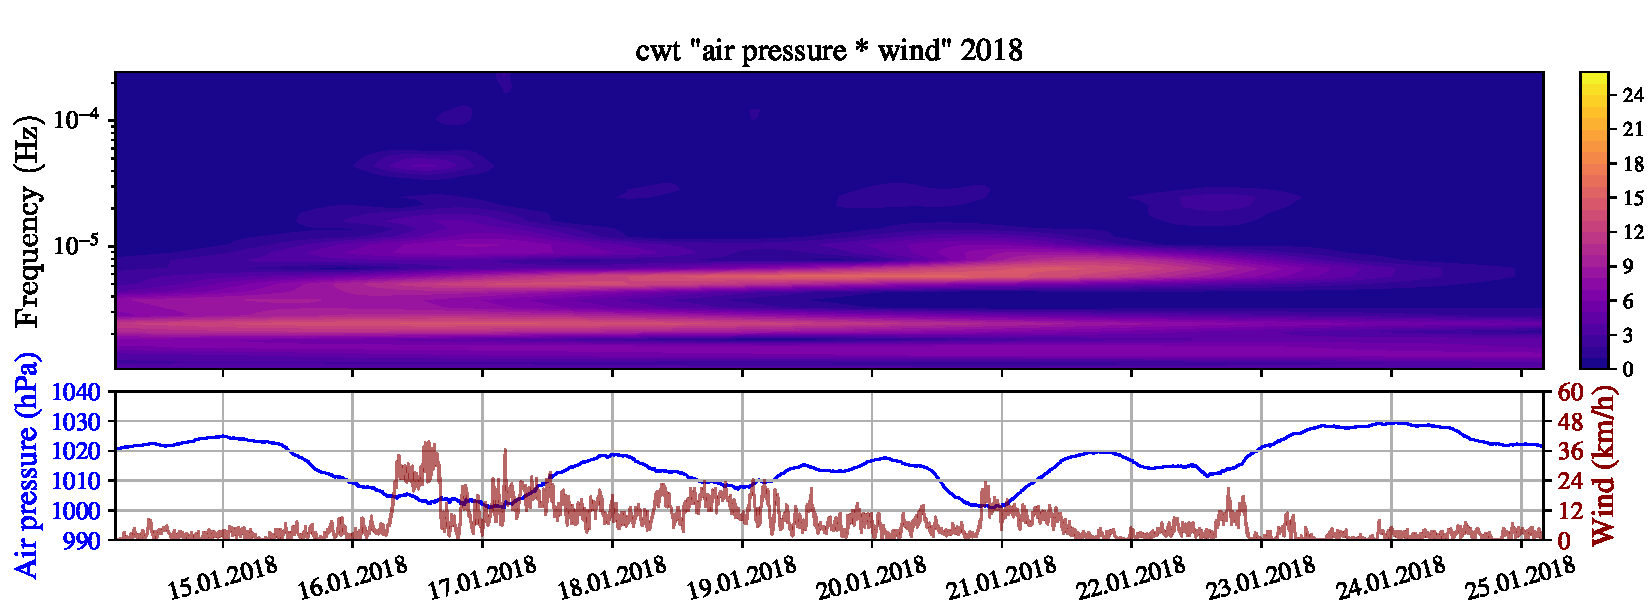
\includegraphics[width=1\textwidth]{papers/wwt/images/storm_airp_wind_zoom2.pdf}
	\caption{Cwt und Rohdaten Strumtief {\em Evi}  und {\em Friedricke} 2018}
	\label{fig:cwt_storm_zoom2}
\end{figure}



\section{Schlussfolgerung}
\rhead{Schlussfolgerung}

Mit dem Versuch, die Wavelet-Transformation im Bereich der Wetteranalyse nützlich anzuwenden, zeigt sich, dass dies durchaus möglich ist.
In der Anwendung mit dem Phänomen der Winterstürme wurde die Wavelet-Transformation oder genauer die stetige Wavelet-Transformation erfolgreich eingesetzt.
Es können zwei Hypothesen aufgestellt werden:
\begin{itemize}
	\item Die periodischen Tagesverläufe bei konstanten Wetterverhältnissen führen dazu, dass die Wavelet-Koeffizienten der \textit{cwt} bei dieser Frequenz deutlich ansteigen (\ref{Freq}).
	
	\item Nicht periodische Ereignisse äussern sich durch das korrelierte Auftreten bei der Betrachtung mehrerer Datenkanäle. Dies kann mit dem Produkt der Wavelet-Koeffizienten oder eben der Kovarianz analysiert werden (\ref{burglind}).
\end{itemize}


Damit ist selbstverständlich noch nichts abschliessend bewiesen. Die Hypothesen müssten detaillierter analysiert werden.
Auch sollte die Methode weiterführend auf andere meteorologische Ereignisse angewandt werden.
Zum Beispiel könnte man versuchen, Gewitter zu detektieren.
Falls sich diese Methode für mehrere Phänomene beweisen lässt, ist eine praktische Anwendung möglich und durchaus vorstellbar. 

\section{Anhang}
Anbei in Abbildung \ref{fig:python-plot-code} und \ref{fig:python-plot-code2} der verwendete Code zum Plotten der Abbildung \ref{fig:cwt_storm}.

\begin{figure}[h]
	\centering
	\lstinputlisting[language=Python,firstline = 1, lastline = 39, numbers=left, firstnumber=1, style = Python]{papers/wwt/code/plot_burglind.py}
	\caption{Python Codeausschnitt}
	\label{fig:python-plot-code}
\end{figure}
\begin{figure}[h]
	\centering
	\lstinputlisting[language=Python,firstline = 40, lastline = 91, firstnumber=40, numbers=left,style = Python]{papers/wwt/code/plot_burglind.py}
	\caption{Python Codeausschnitt}
	\label{fig:python-plot-code2}
\end{figure}
 
 \newpage

\printbibliography[heading=subbibliography]
\end{refsection}

%
% main.tex -- Paper zum Thema wwt
%
% (c) 2019 Michael Schmid, Hochschule Rapperswil
%
\chapter{Wetter-Wavelet-Transformation\label{chapter:wwt}}
\lhead{Wetter-Wavelet-Transformation}
\begin{refsection}
\chapterauthor{Michael Schmid}



\definecolor{codegreen}{rgb}{0,0.6,0}
\definecolor{codegray}{rgb}{0.5,0.5,0.5}
\definecolor{codepurple}{rgb}{0.58,0,0.82}
\definecolor{backcolour}{rgb}{0.95,0.95,0.92}

\lstdefinestyle{mystyle}{
	backgroundcolor=\color{backcolour},   
	commentstyle=\color{codegreen},
	keywordstyle=\color{magenta},
	numberstyle=\tiny\color{codegray},
	stringstyle=\color{codepurple},
	basicstyle=\footnotesize,
	breakatwhitespace=false,         
	breaklines=true,                 
	captionpos=b,                    
	keepspaces=true,                 
	numbers=left,                    
	numbersep=2pt,                  
	showspaces=false,                
	showstringspaces=false,
	showtabs=false,                  
	tabsize=2
}
\lstset{style=mystyle}
\lstdefinestyle{mystyle}{
	morekeywords={cwt,contourf,datetick}
}


\section{Einführung}
\rhead{Einführung}


Seit Langem konsultiere ich meine aktuellen Wetterdaten über eine eher unübliche Internetseite.
Dabei handelt es sich um eine privat geführte Wetterstation, welche die gemessenen Daten im Internet grafisch darstellt.
Die Daten werden auch tabellarisch zur Verfügung gestellt.
Das Feature, welches ich bis anhin am regelmässigsten nutzte, war die grafische Darstellung der aktuellen Wetterdaten über den Zeitraum der letzten 24 Stunden.
Bei speziellen Ereignissen im Wetterverlauf fielen mir besondere und wiederkehrende Charakteristiken auf.
\\

Nach der Einführung in die Theorie der Wavelets kam mir die Idee, solche Wetterphänomene mit einer geeigneten Wavelet Transformation zu detektieren.
In diesem Paper wird einerseits auf die theoretischen Grundlagen der angewandten Methoden zurückgegriffen sowie die besprochenen meteorologischen Phänomene kurz erläutert. 
Weiterführend wird auf die verwendeten Methoden, auch in der praktischen Anwendung, vertieft eingegangen.
Ein besonderes Augenmerk wird auf die allgemeine Vorgehensweise sowie deren Schwierigkeiten gelegt.
\\




\section{Wetterstation Seegräben}
\rhead{Wetterstation Seegräben}

Die angesprochene Wetterstation in der Gemeinde Seegräben im Kanton Zürich ist mit einer DAVIS Vantage Pro2 6153 \cite{online:davisinstruments} realisiert worden.
Sie verfügt über Sensoren für die Temperatur, Feuchtigkeit, Geschwindigkeit und Richtung des Windes sowie für den Niederschlag. 
Durch diese Sensoren werden folgende Daten aufgezeichnet:


\begin{itemize}
	\item \textbf{Aussentemperatur} in Grad Celsius
	\item \textbf{Relative Luftfeuchtigkeit} in Prozent
	\item \textbf{Luftdruck} in hPa
	\item \textbf{Windgeschwindigkeit} in km/h, gemittelt über 5 Minuten
	\item \textbf{Windböen} in km/h
	\item \textbf{Windrichtung} nach Himmelsrichtung
	\item \textbf{Regenmenge} in $\text{l/m}^{2}$
\end{itemize}	


Der Thermo- / Feuchtigkeitssensor liegt zusammen mit dem Regenmengenmesser auf 2 Meter über Boden.
Mit einem Abstand von rund 10 Meter zum nächsten Gebäude sind optimale Messbedingungen geschaffen.
Mit einem Mast ist der Windmesser auf 1.5 Meter über dem First eines Gebäudes lokalisiert \space \cite{online:wss}.
Die Daten werden anschliessend mit einer Software von PC-Wetterstation.de weiterverarbeitet und auf der Website \cite{online:wss} veröffentlicht.
Mehr zur Verwendung der Wetterdaten im n\"achsten Abschnitt.

\section{Datenaufarbeitung}
\rhead{Datenaufarbeitung}
Der n\"achste Vorbereitungsschritt zur Wavelet Transformation war die Aufbereitung der zur Verf\"ugung gestellten Daten der Wetterstation. Dazu musste erst analysiert werden, wie die Daten auf der Website dargestellt werden.
\subsection{Wetter-Archiv}
Auf der Website gibt es mehrere Möglichkeiten, sich Wetterdaten aus der Vergangenheit darstellen zu lassen.
In der Kategorie des Archivs auf der Website kann man die Wetterdaten eines gew\"unschten Zeitraums tabellarisch oder grafisch darstellen lassen.
Vom Betreiber der Website steht keine Funktion zur Verfügung, welche es erlaubt, die Daten offiziell und automatisch herunterzuladen.
\subsection{Datenerfassung}
Da f\"ur die angestrebte Anwendung eine m\"oglichst hohe Aufl\"osung der jeweiligen Daten erforderlich ist, mussten die Daten im Zeitraum von einem Tag dargestellt werden.
Dies hatte zur Folge, dass man f\"ur jeden Tag eine Tabelle auf dem Archiv der Website \"offnen musste. Man hätte anschliessend die Daten mit copy and paste in eine Excel-Tabelle einf\"ugen können. Daher wurde  entschieden, ein Programm zu schreiben, welches diese Aufgabe automatisieren sollte.
Als Programmiersprache wurde hierf\"ur Python gewählt.


Mit der Pandas Library und der Funktion \texttt{'read\_html'} \space konnten die Daten direkt aus dem Python Programm von der Website heruntergeladen werden.
Entscheidend für das Gelingen dieser Teilaufgabe war, dass die URL-Links der einzelnen Tage stets regelmässig aufgebaut sind:
\\
\\
$$\centering{\textit{https://www.wetter-seegraeben.ch/uploads/insert.php?insert=\textbf{20190701}.htm}}$$
\\
Wie zu sehen ist, wird der Link mit dem Datum regelmässig aufgebaut. Somit konnten die entsprechenden Links mit mehreren While-Schleife zusammengesetzt werden.
In der Abbildung \ref{fig:python-code} ist der wesentliche Ausschnitt aus dem Python Code dargestellt.
\begin{figure}
	\centering
	\lstinputlisting[language=Python,firstline=1,lastline=16,numbers=left,style = Python]{papers/wwt/code/get_data.py}
	\caption{Python Codeausschnitt}
	\label{fig:python-code}
\end{figure}
Die Daten konnten im nächsten Schritt in einer Excel-Tabelle abgespeichert werden.
Dort folgte der letzte Feinschliff; d.h. alle überflüssigen Kopfzeilen und Statistiken wurden entfernt.

\subsubsection{Unregelmässigkeiten der Wetterstation}
Bei der Datenerfassung durch das eben beschriebene Python Programm wurden einige Unregelmässigkeiten der Wetterstation beobachtet.
Das Programm wird jeweils durch eine Fehlermeldung abgebrochen, wenn der angegebene Link nicht abrufbar ist. 
So fiel auf, dass unregelmässig auf das Jahr verteilt, Daten von gewissen Tagen fehlten. Es stellte sich heraus, dass hinter dem eigentlich korrektem Link die entsprechende Internetseite nicht zur Verfügung steht.
Wird manuell auf der Website nach diesem Tag gesucht, kann nichts gefunden werden.
Dies trat teilweise sogar in Abschnitten von mehreren Tagen auf.
Wie sich später herausstellte, traten die fehlenden Tagen nicht zu den Zeitpunkten auf, die mich interessierten.


\subsection{Datendarstellung}
Die Darstellung der gewonnenen Daten konnte einfach mittels Python realisiert werden.
Anbei in Abbildung \ref{fig:rawdata} der Plot der Rohdaten aus dem Jahre 2018, wobei nur jeder zehnte Messpunkt verwendet wurde.
Diese Rohdaten dienten als Grundlage für alle weiteren Berechnungen. 
\begin{figure}
	\centering
	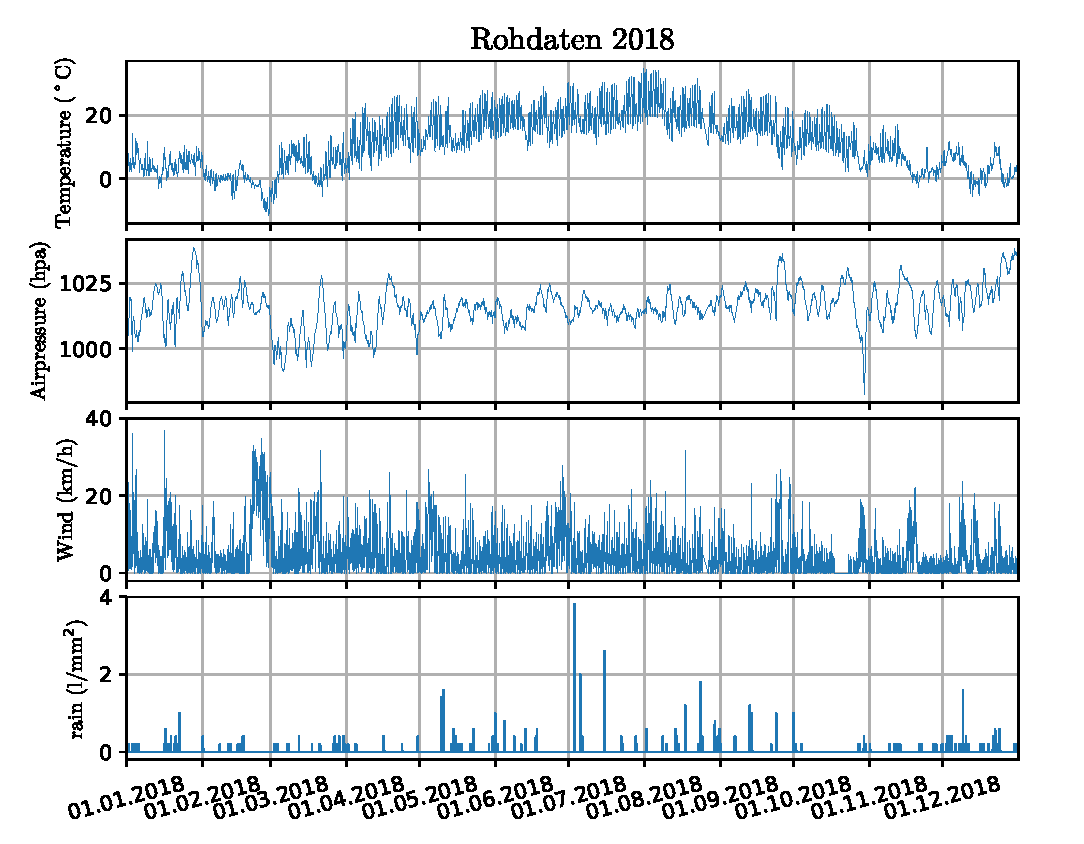
\includegraphics[width=1\textwidth]{papers/wwt/images/raw.pdf}
	\caption{Rohdaten 2018}
	\label{fig:rawdata}
\end{figure}


\section{Stetige Wavelet-Transformation}
\rhead{Stetige Wavelet-Transformation}
Die theoretischen Grundlagen rund um die stetige Wavelet-Transformation wurden im Kapitel \ref{chapter:cwt} genaustens erläutert. 
In diesem Abschnitt der Seminararbeit wird öfters auf die Theorie des angesprochenen Kapitels \ref{chapter:cwt} referenziert ohne diese genauer zu erläutern. 

Für eine m"oglichst aussagekräftige Untersuchung der Signale, in welcher so viele Informationen gewonnen werden sollten wie m"oglich, eignet sich die stetige Wavelet-Transformation (folgend noch kurz \textit{cwt} aus dem Englischen "continuous wavelet transform"). 
Regelmässig auftretende Frequenzen können dank der \textit{cwt} gefunden und zusätzlich einem Zeitraum zugeordnet werden.
\subsection{Das verwendete Wavelet}
In
\begin{equation}
\mathcal{W}f (a,b)
=
\langle f,\psi_{a,b}\rangle
=
\frac{1}{\sqrt{|a|}}\int_{-\infty}^\infty f(t)\,\overline{
	\psi\biggl(\frac{t-b}{a}\biggr)}\,dt
\label{eq:cwt1}
\end{equation}
erkennt man die grundlegende Formel der \textit{cwt}.
Wobei das $\psi_{a,b}$ für das Mutter-Wavelet steht, welches mit dem Koeffizienten $a$ skaliert und mit $b$ verschoben wird.

Als Mutter-Wavelet wurde 
\begin{equation}
\psi_{Gabor}(t) =  c_{\sigma} e^{-\frac{1}{2}t^2} \biggl(e^{i \sigma t}- e^{-\frac{1}{2} \sigma^2} \biggr)
\label{eq:morlet}
\end{equation} \cite{online:Morlet}
verwendet, welches auch als das analytische Gabor-Wavelet bekannt ist.
Dabei gibt $\sigma$ an, wie hoch die Frequenz ist und dementsprechend auch, wie viele lokale Maxima und Minima innerhalb des Gauss'schen Fensters das Mutter-Wavelet existieren.
Weiter ist $c_{\sigma}$ eine reelle Konstante und dient zur Erf"ullung der Zulässigkeitsbedingungen in der Definition \ref{cwt:zulaessig}.
Das Morlet-Wavelet wird in der Abbildung \ref{fig:gabor_plot} \space dargestellt und $\sigma$ wurde auf 5 gesetzt.

\begin{figure}
\centering
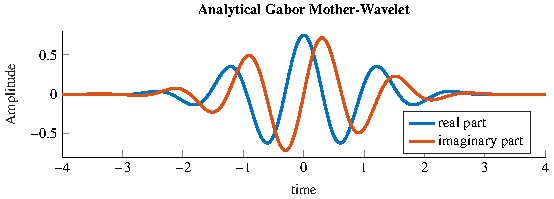
\includegraphics[width=1\textwidth]{papers/wwt/images/gabor.pdf}
\caption{Analytisches Gabor Mutter-Wavelet}
\label{fig:gabor_plot}
\end{figure}

Weiter ist zu erwähnen, dass das eben gezeigte Gabor Wavelet der referenzierten Quelle entnommen wurde. Ob Matlab die selbe Form verwendet, konnte nicht abschliessend geklärt werden.

\subsection{Berechung mit Matlab}
Die Berechnung der \textit{cwt} wurde mit der numerischen Berechnungs-Software Matlab durchgeführt.
Die dafür verwendete Funktion war die cwt()-Funktion.
Die Funktion arbeitete bei korrekter Parametrisierung wie gewünscht.
Falls man verstehen möchte wie die Funktion genau rechnet, muss man sich mit einer eher dürftigen Dokumentation herumschlagen.
Folgende Parameter wurden verwendet
\lstinputlisting[language=Matlab,firstline=1,lastline=1,  numbers=left, style = mystyle]{papers/wwt/code/matlab.m}
\label{fig:matlab_code_cwt}
wobei Matlab das Gabor-Wavelet als \texttt{'amor'} bezeichnet, mit \texttt{'VoicesPerOctave'} konnte die Genauigkeit erhöht werden und die Variable \texttt{'fs'} beschreibt die Abtastfrequenz der Messsignale.
Bei den Rückgabewerten werden die Wavelet-Werte in \texttt{'wt'} als komplexe Matrix und die approximierten Frequenzen in \texttt{'F'} abgespeichert.

Anstelle des Skalierungsfaktors $a$ in der Gleichung \ref{eq:cwt} berechnet Matlab eine approximierte Frequenz und gibt diese zurück.
Für jeden verwendeten Skalierungsfaktor $a$ wird eine Sinuskurve gesucht, die am ehesten mit der Frequenz des entsprechenden Wavelets übereinstimmt.
Siehe das Beispiel mit einem Daubechies Wavelet der Nummer 7 in der Abbildung \ref{fig:centerf}.
Dies dient dazu den Wavelet-Koeffizienten einer Frequenz zuzuordnen. 
Aus dem verwendeten Skalierungsfaktor $a$ könnte auf die Schnelle keine Information entnommen werden.
\begin{figure}[h]
	\centering
	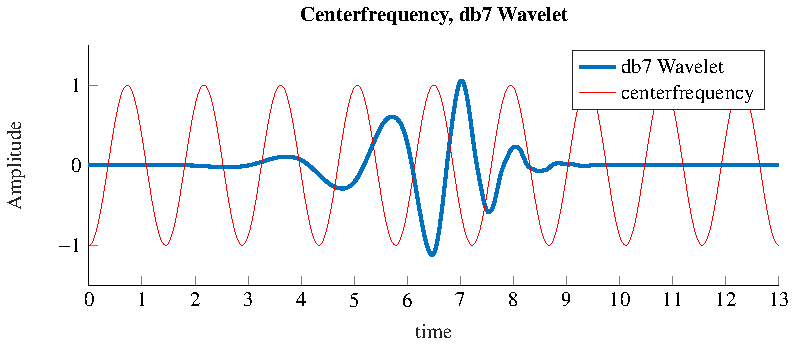
\includegraphics[width=1\textwidth]{papers/wwt/images/centerf.pdf}
	\caption{Approximierte Frequenz eines db7-Wavelet}
	\label{fig:centerf}
\end{figure}

\subsection{Verifikation der approximierten Frequenz}
\label{Freq}
Diese approximierte Frequenz konnte man mit den geeigneten Daten aus der aktuellen Anwendung der Wetterdaten sehr gut verifizieren.
Der Temperaturverlauf während einer Hochdruckphase ist sehr regelmässig und man sollte den 24 Stunden Tagesverlauf exakt erkennen.

Dank der Regelm"assigkeit des Temperaturverlaufs sieht man im \textit{cwt}-Plot eine Erh"ohung des Wertes bei einer gewissen Frequenz.
Die ausgelesene Frequenz beträgt $f = 1.16\cdot10^{-5} \,\text{Hz}$, die umgerechnet einer Periodendauer von $T = 86206.897\,\text{s}\approx 23\,\text{h }56\,\text{min } 47\,\text{s}$ entspricht.
Damit kann die Frequenz im Rückgabewert der Matlab-Funktion als sehr genau bezeichnet werden.
Dabei kommt weiter dazu, dass nur alle f"unf Minuten ein Datenpunkt aufgenommen wurde und somit die Abweichung zu 24 Stunden kleiner ist als die eigentliche Auflösung.

\begin{figure}[h]
	\centering
	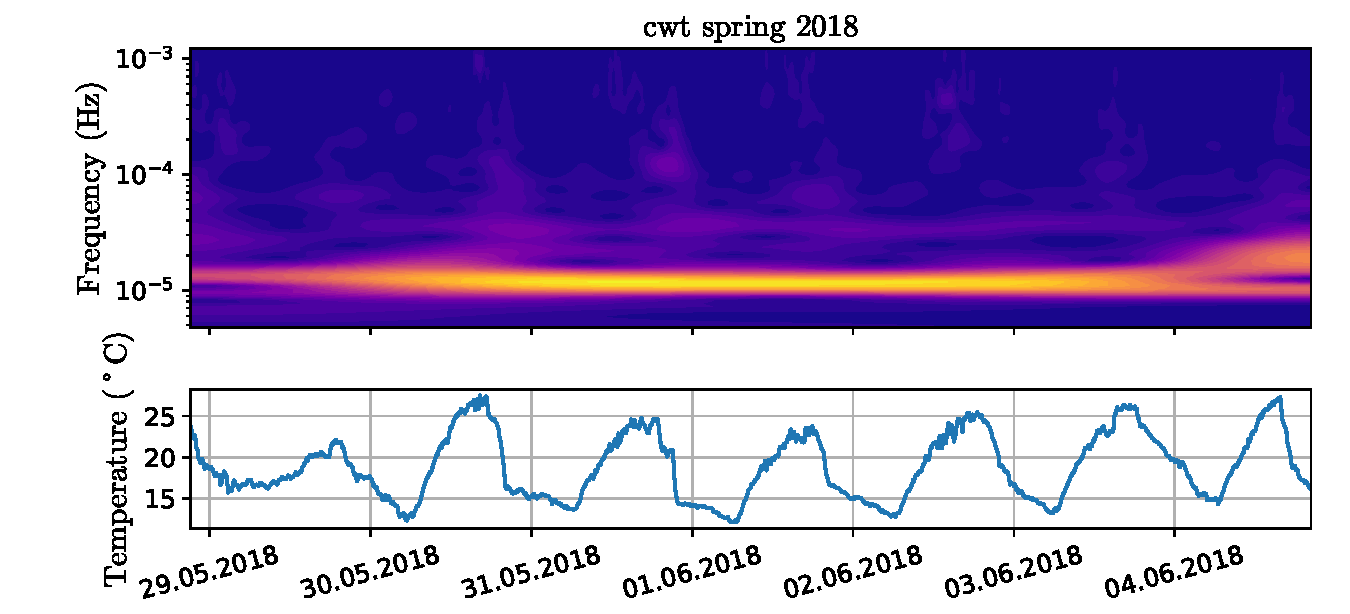
\includegraphics[width=1\textwidth]{papers/wwt/images/data_spring.pdf}
	\caption{Temperaturverlauf und entsprechende cwt}
	\label{fig:cwt_zoom}
\end{figure}



\section{Analyse von Wettereignissen}
\rhead{Analyse von Wetterereignissen}
Aufgrund der Kenntnisse rund um die \textit{cwt} kann angenommen werden, dass ein Wechsel in der Frequenz gut detektiert werden kann.
Bei einer typischen Sturmfront, welche öfters als Wintersturm in den Monaten Dezember und Januar auftreten, zeigten sich bei der Konsultation der Wetterdaten rapide Temperatur- und Luftdruckwechsel sowie ein erhöhtes Windaufkommen.
Das Ziel der Analyse war, solche Ereignisse mittels einer geeigneten \textit{cwt} zu detektieren.
Bei den Rohdaten der Frontdurchgängen erkennt man gemeinsame Wechsel im Wind, der Temperatur sowie dem Luftdruck, daher kann in der Wavelet-Transformation eine erkennbare Antwort erwartet werden. 
Diese korrelierenden auftretenden Frequenzen sollten in der \textit{cwt} sichtbar sein.

\subsection{Parallelen zur Kovarianz}

Um das korrelierende Auftreten der einzelnen Datenkanäle zu verdeutlichen, wurden bei diesen jeweils die zwei zusammengehörenden Koeffizienten der \textit{cwt} miteinander multipliziert. 
Dabei werden die Stellen hervorgehoben, wo beispielsweise der Luftdruck und die Windgeschwindigkeit abhängig voneinander variieren.  
Dies funktioniert besonders gut, da die Werte rasch gegen null gehen falls nur schon einer der beiden Datenverläufe nicht mit dem aktuellen Mutter-Wavelet übereinstimmt.
Genauer betrachtet zeigt dieses Verfahren Ähnlichkeiten mit der Formel
\begin{equation}
COV(X,Y) = \frac{\sum_{i=1}^{N} (x_i- \bar{x})(y_i- \bar{y})}{N-1},
\label{eq:kovarianz}
\end{equation}
der Kovarianz aus der Statistik. Bei dieser Anwendung wird einfach nicht die ganze Zufallsvariable benutzt, sondern nur jeweils die beiden zeitlich übereinstimmenden Werte.

Die Kovarianz zeigt sich nicht nur in dieser Anwendung. Auch schon bei der grundlegenden Formel \ref{eq:cwt1} der \textit{cwt}, kann man gewisse Parallelen sehen. 
In \ref{eq:cwt1} ist die Motivation, die jeweiligen Parameter $a$ und $b$ zu finden, wobei das Mutter-Wavelet und das Signal gemeinsam variieren.
Auch hierfür werden die Produkte der Signale berechnet, auf integriert und gemittelt.
Auch dies ist eine etwas abgewandelte Art der Kovarianz zwischen dem Datensignal und dem Mutter-Wavelet.


Die im Paper angewendete Wavelet-Transformation mit der Idee des Produktes der beiden Datenkanäle,
\begin{equation}
\begin{split}
\mathcal{W}f (a,b)
& =
\biggl<\langle Luftdruck,\psi_{a,b}\rangle, \langle Wind,\psi_{a,b} \rangle \biggr > \\
& = \biggl< \frac{1}{\sqrt{|a|}}\int_{-\infty}^\infty Luftdruck(t)\,\overline{
	\psi\biggl(\frac{t-b}{a}\biggr)}\,dt
,
\frac{1}{\sqrt{|a|}}\int_{-\infty}^\infty Wind(t)\,\overline{
	\psi\biggl(\frac{t-b}{a}\biggr)}\,dt \biggr>
\label{eq:cwt_wwt}
\end{split}
\end{equation}
kann, vorerst nur für den Luftdruck, auf die Kovarianz (Formel \ref{eq:kovarianz}) umgeschrieben werden,

\begin{equation}
COV(Luftdruck, \psi_{a,b})f(a,b) = \frac{\sum_{i=1}^{N} (Luftdruck_i - \overline{Luftdruck})(\psi_{a,b}-  \overline{\psi_{a,b}})}{N-1}.
\end{equation}
Gemäss den Zulässigkeitsbedingungen eines Mutter-Wavelets ist $\overline{\psi_{a,b}} = 0$ (Definition \ref{cwt:zulaessig}). Weiter werden Multiplikationen in Skalarprodukte umgewandelt, somit folgt;
\begin{equation}
COV(Luftdruck, \psi_{a,b})f(a,b) =  \frac{\sum_{i=1}^{N} 
 \langle Luftdruck_i- \overline{Luftdruck},\psi_{a,b}\rangle}{N-1}.
\end{equation}
Weiter Ausmultipliziert
\begin{equation}
COV(Luftdruck, \psi_{a,b})f(a,b) = \frac{\sum_{i=1}^{N} 
\langle Luftdruck_i,\psi_{a,b}\rangle - \langle \overline{Luftdruck},\psi_{a,b}\rangle}{N-1},
\end{equation}
schlussendlich ergibt sich mit $\langle \overline{Luftdruck},\psi_{a,b} \rangle = 0$,
\begin{equation}
COV(Luftdruck, \psi_{a,b})f(a,b) = \frac{\sum_{i=1}^{N} 
	\langle Luftdruck_i,\psi_{a,b}\rangle}{N-1}.
\end{equation}
 Wird noch das Produkt mit dem Wind hinzugenommen
 \begin{equation}
 \begin{split}
\biggl< COV(Luftdruck, \psi_{a,b})f(a,b), COV(Wind), \psi_{a,b})f(a,b) \biggr > \\
=
 \biggl< \frac{\sum_{i=1}^{N} 
 	\langle Luftdruck_i,\psi_{a,b}\rangle}{N-1},\frac{\sum_{i=1}^{N} 
 	\langle Wind_i,\psi_{a,b}\rangle}{N-1} \biggr >,
 \label{eq:cov_wwt}
 \end{split}
 \end{equation}
 wurde die Herleitung von der Wavelet-Transformation in der Formel \ref{eq:cwt_wwt} zum einem äquivalenten Resultat, ohne die Korrekturfaktoren, mit der Kovarianz in der Formel \ref{eq:cov_wwt} gezeigt.



\subsection{Sturmsaison 2018}
\rhead{Sturmsaison 2018}
Bereits bekannt war, dass in der Sturmsaison im Jahre 2018 einige heftige Winterstürme aufgetreten sind.
So wurde bei der Analyse der Daten nur auf diese Periode das Augenmerk gelegt. 
In Abbildung \ref{fig:cwt_storm} \space sieht man die Wavelet-Transformation des Luftdruckes und Windes miteinander multipliziert.
Dies über die Monate Januar und Februar im Jahre 2018 hinweg.
Weiter wird der Luftdruck- und Windverlauf dargestellt.
 
\begin{figure}[h]
	\centering
	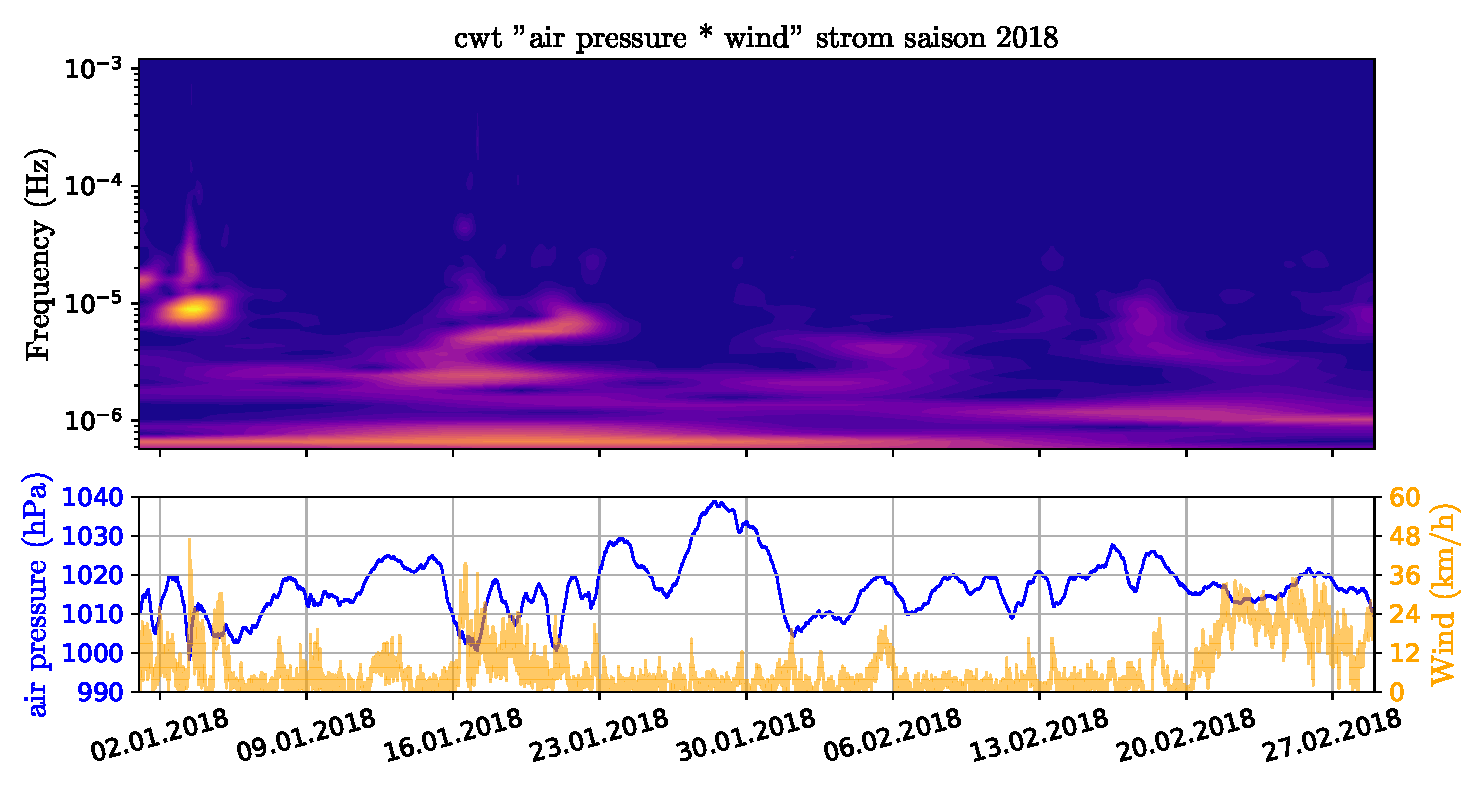
\includegraphics[width=1\textwidth]{papers/wwt/images/storm_airp_wind.pdf}
	\caption{Cwt und Rohdaten Sturmsaison 2018}
	\label{fig:cwt_storm}
\end{figure}

In Abbildung \ref{fig:cwt_storm} \space zeigen sich um den 3. sowie zwischen dem 16. und 23. Januar jeweils gewisse Frequenzen des Windes und des Luftdruckes, die gemeinsam auf die Wavelet-Transformation angesprochen haben.

\subsubsection{Wintersturm {\em Burglind} }
\label{burglind}
Hineingezoomt um den 3. Januar (Abbildung \ref{fig:cwt_storm_zoom}) sind im Rohdatenverlauf die Aktivitäten des Windes und Luftdruckes erkennbar. 
\begin{figure}[b]
	\centering
	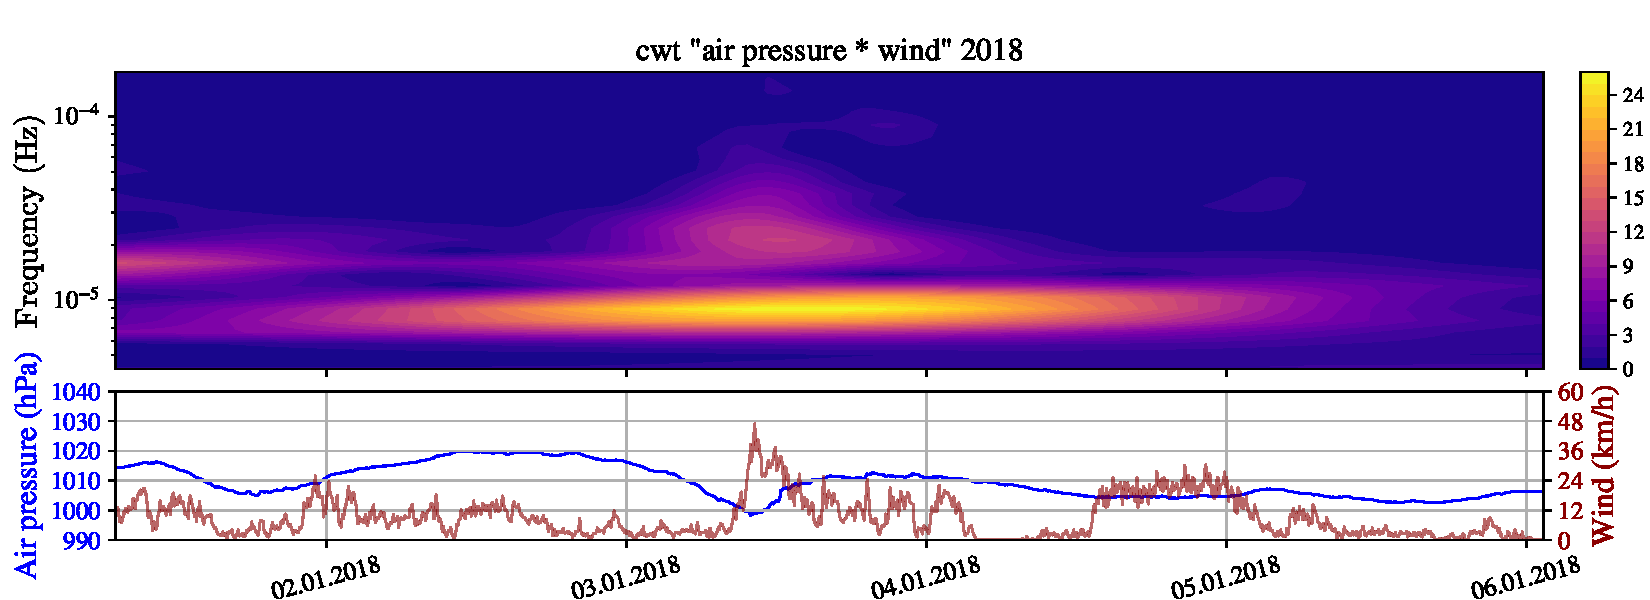
\includegraphics[width=1\textwidth]{papers/wwt/images/storm_airp_wind_zoom.pdf}
	\caption{Cwt und Rohdaten Wintersturm {\em Burglind}  2018}
	\label{fig:cwt_storm_zoom}
\end{figure}
Aus dem Fachbericht \space \cite{Fachbericht:Burglind} von Meteoschweiz war bekannt, dass am Vormittag des 3. Januars 2018 die stärkste Sturmfront seit dem verheerenden Sturm Lothar aus dem Jahre 1999 über die Schweiz zog.
Dabei zeigt sich eindrücklich, wie der Sturmdurchgang in der multiplizierten Wavelet-Transformation hervorgehoben wird.

\subsubsection{Sturmtief {\em Evi}  und {\em Friedricke} }
\label{evi}
Beim zweiten Ereignis zwischen dem 16. und 23. Januar trat die Aktivität nicht mehr so deutlich auf.
Nach dem Sturmarchiv  \cite{online:sturmarchiv} traf am 16. Januar das Sturmtief {\em Evi}  und am 18. Januar das Sturmtief {\em Friedricke} auf Europa. Dabei zeigt sich nach der Amplitude, dass das Sturmtief nicht direkt auf die Schweiz traf, sonder diese lediglich streifte. 

\begin{figure}[h]
	\centering
	\includegraphics[width=1\textwidth]{papers/wwt/images/storm_airp_wind_zoom2.pdf}
	\caption{Cwt und Rohdaten Strumtief {\em Evi}  und {\em Friedricke} 2018}
	\label{fig:cwt_storm_zoom2}
\end{figure}



\section{Schlussfolgerung}
\rhead{Schlussfolgerung}

Mit dem Versuch, die Wavelet-Transformation im Bereich der Wetteranalyse nützlich anzuwenden, zeigt sich, dass dies durchaus möglich ist.
In der Anwendung mit dem Phänomen der Winterstürme wurde die Wavelet-Transformation oder genauer die stetige Wavelet-Transformation erfolgreich eingesetzt.
Es können zwei Hypothesen aufgestellt werden:
\begin{itemize}
	\item Die periodischen Tagesverläufe bei konstanten Wetterverhältnissen führen dazu, dass die Wavelet-Koeffizienten der \textit{cwt} bei dieser Frequenz deutlich ansteigen (\ref{Freq}).
	
	\item Nicht periodische Ereignisse äussern sich durch das korrelierte Auftreten bei der Betrachtung mehrerer Datenkanäle. Dies kann mit dem Produkt der Wavelet-Koeffizienten oder eben der Kovarianz analysiert werden (\ref{burglind}).
\end{itemize}


Damit ist selbstverständlich noch nichts abschliessend bewiesen. Die Hypothesen müssten detaillierter analysiert werden.
Auch sollte die Methode weiterführend auf andere meteorologische Ereignisse angewandt werden.
Zum Beispiel könnte man versuchen, Gewitter zu detektieren.
Falls sich diese Methode für mehrere Phänomene beweisen lässt, ist eine praktische Anwendung möglich und durchaus vorstellbar. 

\section{Anhang}
Anbei in Abbildung \ref{fig:python-plot-code} und \ref{fig:python-plot-code2} der verwendete Code zum Plotten der Abbildung \ref{fig:cwt_storm}.

\begin{figure}[h]
	\centering
	\lstinputlisting[language=Python,firstline = 1, lastline = 39, numbers=left, firstnumber=1, style = Python]{papers/wwt/code/plot_burglind.py}
	\caption{Python Codeausschnitt}
	\label{fig:python-plot-code}
\end{figure}
\begin{figure}[h]
	\centering
	\lstinputlisting[language=Python,firstline = 40, lastline = 91, firstnumber=40, numbers=left,style = Python]{papers/wwt/code/plot_burglind.py}
	\caption{Python Codeausschnitt}
	\label{fig:python-plot-code2}
\end{figure}
 
 \newpage

\printbibliography[heading=subbibliography]
\end{refsection}

%
% main.tex -- Paper zum Thema wwt
%
% (c) 2019 Michael Schmid, Hochschule Rapperswil
%
\chapter{Wetter-Wavelet-Transformation\label{chapter:wwt}}
\lhead{Wetter-Wavelet-Transformation}
\begin{refsection}
\chapterauthor{Michael Schmid}



\definecolor{codegreen}{rgb}{0,0.6,0}
\definecolor{codegray}{rgb}{0.5,0.5,0.5}
\definecolor{codepurple}{rgb}{0.58,0,0.82}
\definecolor{backcolour}{rgb}{0.95,0.95,0.92}

\lstdefinestyle{mystyle}{
	backgroundcolor=\color{backcolour},   
	commentstyle=\color{codegreen},
	keywordstyle=\color{magenta},
	numberstyle=\tiny\color{codegray},
	stringstyle=\color{codepurple},
	basicstyle=\footnotesize,
	breakatwhitespace=false,         
	breaklines=true,                 
	captionpos=b,                    
	keepspaces=true,                 
	numbers=left,                    
	numbersep=2pt,                  
	showspaces=false,                
	showstringspaces=false,
	showtabs=false,                  
	tabsize=2
}
\lstset{style=mystyle}
\lstdefinestyle{mystyle}{
	morekeywords={cwt,contourf,datetick}
}


\section{Einführung}
\rhead{Einführung}


Seit Langem konsultiere ich meine aktuellen Wetterdaten über eine eher unübliche Internetseite.
Dabei handelt es sich um eine privat geführte Wetterstation, welche die gemessenen Daten im Internet grafisch darstellt.
Die Daten werden auch tabellarisch zur Verfügung gestellt.
Das Feature, welches ich bis anhin am regelmässigsten nutzte, war die grafische Darstellung der aktuellen Wetterdaten über den Zeitraum der letzten 24 Stunden.
Bei speziellen Ereignissen im Wetterverlauf fielen mir besondere und wiederkehrende Charakteristiken auf.
\\

Nach der Einführung in die Theorie der Wavelets kam mir die Idee, solche Wetterphänomene mit einer geeigneten Wavelet Transformation zu detektieren.
In diesem Paper wird einerseits auf die theoretischen Grundlagen der angewandten Methoden zurückgegriffen sowie die besprochenen meteorologischen Phänomene kurz erläutert. 
Weiterführend wird auf die verwendeten Methoden, auch in der praktischen Anwendung, vertieft eingegangen.
Ein besonderes Augenmerk wird auf die allgemeine Vorgehensweise sowie deren Schwierigkeiten gelegt.
\\




\section{Wetterstation Seegräben}
\rhead{Wetterstation Seegräben}

Die angesprochene Wetterstation in der Gemeinde Seegräben im Kanton Zürich ist mit einer DAVIS Vantage Pro2 6153 \cite{online:davisinstruments} realisiert worden.
Sie verfügt über Sensoren für die Temperatur, Feuchtigkeit, Geschwindigkeit und Richtung des Windes sowie für den Niederschlag. 
Durch diese Sensoren werden folgende Daten aufgezeichnet:


\begin{itemize}
	\item \textbf{Aussentemperatur} in Grad Celsius
	\item \textbf{Relative Luftfeuchtigkeit} in Prozent
	\item \textbf{Luftdruck} in hPa
	\item \textbf{Windgeschwindigkeit} in km/h, gemittelt über 5 Minuten
	\item \textbf{Windböen} in km/h
	\item \textbf{Windrichtung} nach Himmelsrichtung
	\item \textbf{Regenmenge} in $\text{l/m}^{2}$
\end{itemize}	


Der Thermo- / Feuchtigkeitssensor liegt zusammen mit dem Regenmengenmesser auf 2 Meter über Boden.
Mit einem Abstand von rund 10 Meter zum nächsten Gebäude sind optimale Messbedingungen geschaffen.
Mit einem Mast ist der Windmesser auf 1.5 Meter über dem First eines Gebäudes lokalisiert \space \cite{online:wss}.
Die Daten werden anschliessend mit einer Software von PC-Wetterstation.de weiterverarbeitet und auf der Website \cite{online:wss} veröffentlicht.
Mehr zur Verwendung der Wetterdaten im n\"achsten Abschnitt.

\section{Datenaufarbeitung}
\rhead{Datenaufarbeitung}
Der n\"achste Vorbereitungsschritt zur Wavelet Transformation war die Aufbereitung der zur Verf\"ugung gestellten Daten der Wetterstation. Dazu musste erst analysiert werden, wie die Daten auf der Website dargestellt werden.
\subsection{Wetter-Archiv}
Auf der Website gibt es mehrere Möglichkeiten, sich Wetterdaten aus der Vergangenheit darstellen zu lassen.
In der Kategorie des Archivs auf der Website kann man die Wetterdaten eines gew\"unschten Zeitraums tabellarisch oder grafisch darstellen lassen.
Vom Betreiber der Website steht keine Funktion zur Verfügung, welche es erlaubt, die Daten offiziell und automatisch herunterzuladen.
\subsection{Datenerfassung}
Da f\"ur die angestrebte Anwendung eine m\"oglichst hohe Aufl\"osung der jeweiligen Daten erforderlich ist, mussten die Daten im Zeitraum von einem Tag dargestellt werden.
Dies hatte zur Folge, dass man f\"ur jeden Tag eine Tabelle auf dem Archiv der Website \"offnen musste. Man hätte anschliessend die Daten mit copy and paste in eine Excel-Tabelle einf\"ugen können. Daher wurde  entschieden, ein Programm zu schreiben, welches diese Aufgabe automatisieren sollte.
Als Programmiersprache wurde hierf\"ur Python gewählt.


Mit der Pandas Library und der Funktion \texttt{'read\_html'} \space konnten die Daten direkt aus dem Python Programm von der Website heruntergeladen werden.
Entscheidend für das Gelingen dieser Teilaufgabe war, dass die URL-Links der einzelnen Tage stets regelmässig aufgebaut sind:
\\
\\
$$\centering{\textit{https://www.wetter-seegraeben.ch/uploads/insert.php?insert=\textbf{20190701}.htm}}$$
\\
Wie zu sehen ist, wird der Link mit dem Datum regelmässig aufgebaut. Somit konnten die entsprechenden Links mit mehreren While-Schleife zusammengesetzt werden.
In der Abbildung \ref{fig:python-code} ist der wesentliche Ausschnitt aus dem Python Code dargestellt.
\begin{figure}
	\centering
	\lstinputlisting[language=Python,firstline=1,lastline=16,numbers=left,style = Python]{papers/wwt/code/get_data.py}
	\caption{Python Codeausschnitt}
	\label{fig:python-code}
\end{figure}
Die Daten konnten im nächsten Schritt in einer Excel-Tabelle abgespeichert werden.
Dort folgte der letzte Feinschliff; d.h. alle überflüssigen Kopfzeilen und Statistiken wurden entfernt.

\subsubsection{Unregelmässigkeiten der Wetterstation}
Bei der Datenerfassung durch das eben beschriebene Python Programm wurden einige Unregelmässigkeiten der Wetterstation beobachtet.
Das Programm wird jeweils durch eine Fehlermeldung abgebrochen, wenn der angegebene Link nicht abrufbar ist. 
So fiel auf, dass unregelmässig auf das Jahr verteilt, Daten von gewissen Tagen fehlten. Es stellte sich heraus, dass hinter dem eigentlich korrektem Link die entsprechende Internetseite nicht zur Verfügung steht.
Wird manuell auf der Website nach diesem Tag gesucht, kann nichts gefunden werden.
Dies trat teilweise sogar in Abschnitten von mehreren Tagen auf.
Wie sich später herausstellte, traten die fehlenden Tagen nicht zu den Zeitpunkten auf, die mich interessierten.


\subsection{Datendarstellung}
Die Darstellung der gewonnenen Daten konnte einfach mittels Python realisiert werden.
Anbei in Abbildung \ref{fig:rawdata} der Plot der Rohdaten aus dem Jahre 2018, wobei nur jeder zehnte Messpunkt verwendet wurde.
Diese Rohdaten dienten als Grundlage für alle weiteren Berechnungen. 
\begin{figure}
	\centering
	\includegraphics[width=1\textwidth]{papers/wwt/images/raw.pdf}
	\caption{Rohdaten 2018}
	\label{fig:rawdata}
\end{figure}


\section{Stetige Wavelet-Transformation}
\rhead{Stetige Wavelet-Transformation}
Die theoretischen Grundlagen rund um die stetige Wavelet-Transformation wurden im Kapitel \ref{chapter:cwt} genaustens erläutert. 
In diesem Abschnitt der Seminararbeit wird öfters auf die Theorie des angesprochenen Kapitels \ref{chapter:cwt} referenziert ohne diese genauer zu erläutern. 

Für eine m"oglichst aussagekräftige Untersuchung der Signale, in welcher so viele Informationen gewonnen werden sollten wie m"oglich, eignet sich die stetige Wavelet-Transformation (folgend noch kurz \textit{cwt} aus dem Englischen "continuous wavelet transform"). 
Regelmässig auftretende Frequenzen können dank der \textit{cwt} gefunden und zusätzlich einem Zeitraum zugeordnet werden.
\subsection{Das verwendete Wavelet}
In
\begin{equation}
\mathcal{W}f (a,b)
=
\langle f,\psi_{a,b}\rangle
=
\frac{1}{\sqrt{|a|}}\int_{-\infty}^\infty f(t)\,\overline{
	\psi\biggl(\frac{t-b}{a}\biggr)}\,dt
\label{eq:cwt1}
\end{equation}
erkennt man die grundlegende Formel der \textit{cwt}.
Wobei das $\psi_{a,b}$ für das Mutter-Wavelet steht, welches mit dem Koeffizienten $a$ skaliert und mit $b$ verschoben wird.

Als Mutter-Wavelet wurde 
\begin{equation}
\psi_{Gabor}(t) =  c_{\sigma} e^{-\frac{1}{2}t^2} \biggl(e^{i \sigma t}- e^{-\frac{1}{2} \sigma^2} \biggr)
\label{eq:morlet}
\end{equation} \cite{online:Morlet}
verwendet, welches auch als das analytische Gabor-Wavelet bekannt ist.
Dabei gibt $\sigma$ an, wie hoch die Frequenz ist und dementsprechend auch, wie viele lokale Maxima und Minima innerhalb des Gauss'schen Fensters das Mutter-Wavelet existieren.
Weiter ist $c_{\sigma}$ eine reelle Konstante und dient zur Erf"ullung der Zulässigkeitsbedingungen in der Definition \ref{cwt:zulaessig}.
Das Morlet-Wavelet wird in der Abbildung \ref{fig:gabor_plot} \space dargestellt und $\sigma$ wurde auf 5 gesetzt.

\begin{figure}
\centering
\includegraphics[width=1\textwidth]{papers/wwt/images/gabor.pdf}
\caption{Analytisches Gabor Mutter-Wavelet}
\label{fig:gabor_plot}
\end{figure}

Weiter ist zu erwähnen, dass das eben gezeigte Gabor Wavelet der referenzierten Quelle entnommen wurde. Ob Matlab die selbe Form verwendet, konnte nicht abschliessend geklärt werden.

\subsection{Berechung mit Matlab}
Die Berechnung der \textit{cwt} wurde mit der numerischen Berechnungs-Software Matlab durchgeführt.
Die dafür verwendete Funktion war die cwt()-Funktion.
Die Funktion arbeitete bei korrekter Parametrisierung wie gewünscht.
Falls man verstehen möchte wie die Funktion genau rechnet, muss man sich mit einer eher dürftigen Dokumentation herumschlagen.
Folgende Parameter wurden verwendet
\lstinputlisting[language=Matlab,firstline=1,lastline=1,  numbers=left, style = mystyle]{papers/wwt/code/matlab.m}
\label{fig:matlab_code_cwt}
wobei Matlab das Gabor-Wavelet als \texttt{'amor'} bezeichnet, mit \texttt{'VoicesPerOctave'} konnte die Genauigkeit erhöht werden und die Variable \texttt{'fs'} beschreibt die Abtastfrequenz der Messsignale.
Bei den Rückgabewerten werden die Wavelet-Werte in \texttt{'wt'} als komplexe Matrix und die approximierten Frequenzen in \texttt{'F'} abgespeichert.

Anstelle des Skalierungsfaktors $a$ in der Gleichung \ref{eq:cwt} berechnet Matlab eine approximierte Frequenz und gibt diese zurück.
Für jeden verwendeten Skalierungsfaktor $a$ wird eine Sinuskurve gesucht, die am ehesten mit der Frequenz des entsprechenden Wavelets übereinstimmt.
Siehe das Beispiel mit einem Daubechies Wavelet der Nummer 7 in der Abbildung \ref{fig:centerf}.
Dies dient dazu den Wavelet-Koeffizienten einer Frequenz zuzuordnen. 
Aus dem verwendeten Skalierungsfaktor $a$ könnte auf die Schnelle keine Information entnommen werden.
\begin{figure}[h]
	\centering
	\includegraphics[width=1\textwidth]{papers/wwt/images/centerf.pdf}
	\caption{Approximierte Frequenz eines db7-Wavelet}
	\label{fig:centerf}
\end{figure}

\subsection{Verifikation der approximierten Frequenz}
\label{Freq}
Diese approximierte Frequenz konnte man mit den geeigneten Daten aus der aktuellen Anwendung der Wetterdaten sehr gut verifizieren.
Der Temperaturverlauf während einer Hochdruckphase ist sehr regelmässig und man sollte den 24 Stunden Tagesverlauf exakt erkennen.

Dank der Regelm"assigkeit des Temperaturverlaufs sieht man im \textit{cwt}-Plot eine Erh"ohung des Wertes bei einer gewissen Frequenz.
Die ausgelesene Frequenz beträgt $f = 1.16\cdot10^{-5} \,\text{Hz}$, die umgerechnet einer Periodendauer von $T = 86206.897\,\text{s}\approx 23\,\text{h }56\,\text{min } 47\,\text{s}$ entspricht.
Damit kann die Frequenz im Rückgabewert der Matlab-Funktion als sehr genau bezeichnet werden.
Dabei kommt weiter dazu, dass nur alle f"unf Minuten ein Datenpunkt aufgenommen wurde und somit die Abweichung zu 24 Stunden kleiner ist als die eigentliche Auflösung.

\begin{figure}[h]
	\centering
	\includegraphics[width=1\textwidth]{papers/wwt/images/data_spring.pdf}
	\caption{Temperaturverlauf und entsprechende cwt}
	\label{fig:cwt_zoom}
\end{figure}



\section{Analyse von Wettereignissen}
\rhead{Analyse von Wetterereignissen}
Aufgrund der Kenntnisse rund um die \textit{cwt} kann angenommen werden, dass ein Wechsel in der Frequenz gut detektiert werden kann.
Bei einer typischen Sturmfront, welche öfters als Wintersturm in den Monaten Dezember und Januar auftreten, zeigten sich bei der Konsultation der Wetterdaten rapide Temperatur- und Luftdruckwechsel sowie ein erhöhtes Windaufkommen.
Das Ziel der Analyse war, solche Ereignisse mittels einer geeigneten \textit{cwt} zu detektieren.
Bei den Rohdaten der Frontdurchgängen erkennt man gemeinsame Wechsel im Wind, der Temperatur sowie dem Luftdruck, daher kann in der Wavelet-Transformation eine erkennbare Antwort erwartet werden. 
Diese korrelierenden auftretenden Frequenzen sollten in der \textit{cwt} sichtbar sein.

\subsection{Parallelen zur Kovarianz}

Um das korrelierende Auftreten der einzelnen Datenkanäle zu verdeutlichen, wurden bei diesen jeweils die zwei zusammengehörenden Koeffizienten der \textit{cwt} miteinander multipliziert. 
Dabei werden die Stellen hervorgehoben, wo beispielsweise der Luftdruck und die Windgeschwindigkeit abhängig voneinander variieren.  
Dies funktioniert besonders gut, da die Werte rasch gegen null gehen falls nur schon einer der beiden Datenverläufe nicht mit dem aktuellen Mutter-Wavelet übereinstimmt.
Genauer betrachtet zeigt dieses Verfahren Ähnlichkeiten mit der Formel
\begin{equation}
COV(X,Y) = \frac{\sum_{i=1}^{N} (x_i- \bar{x})(y_i- \bar{y})}{N-1},
\label{eq:kovarianz}
\end{equation}
der Kovarianz aus der Statistik. Bei dieser Anwendung wird einfach nicht die ganze Zufallsvariable benutzt, sondern nur jeweils die beiden zeitlich übereinstimmenden Werte.

Die Kovarianz zeigt sich nicht nur in dieser Anwendung. Auch schon bei der grundlegenden Formel \ref{eq:cwt1} der \textit{cwt}, kann man gewisse Parallelen sehen. 
In \ref{eq:cwt1} ist die Motivation, die jeweiligen Parameter $a$ und $b$ zu finden, wobei das Mutter-Wavelet und das Signal gemeinsam variieren.
Auch hierfür werden die Produkte der Signale berechnet, auf integriert und gemittelt.
Auch dies ist eine etwas abgewandelte Art der Kovarianz zwischen dem Datensignal und dem Mutter-Wavelet.


Die im Paper angewendete Wavelet-Transformation mit der Idee des Produktes der beiden Datenkanäle,
\begin{equation}
\begin{split}
\mathcal{W}f (a,b)
& =
\biggl<\langle Luftdruck,\psi_{a,b}\rangle, \langle Wind,\psi_{a,b} \rangle \biggr > \\
& = \biggl< \frac{1}{\sqrt{|a|}}\int_{-\infty}^\infty Luftdruck(t)\,\overline{
	\psi\biggl(\frac{t-b}{a}\biggr)}\,dt
,
\frac{1}{\sqrt{|a|}}\int_{-\infty}^\infty Wind(t)\,\overline{
	\psi\biggl(\frac{t-b}{a}\biggr)}\,dt \biggr>
\label{eq:cwt_wwt}
\end{split}
\end{equation}
kann, vorerst nur für den Luftdruck, auf die Kovarianz (Formel \ref{eq:kovarianz}) umgeschrieben werden,

\begin{equation}
COV(Luftdruck, \psi_{a,b})f(a,b) = \frac{\sum_{i=1}^{N} (Luftdruck_i - \overline{Luftdruck})(\psi_{a,b}-  \overline{\psi_{a,b}})}{N-1}.
\end{equation}
Gemäss den Zulässigkeitsbedingungen eines Mutter-Wavelets ist $\overline{\psi_{a,b}} = 0$ (Definition \ref{cwt:zulaessig}). Weiter werden Multiplikationen in Skalarprodukte umgewandelt, somit folgt;
\begin{equation}
COV(Luftdruck, \psi_{a,b})f(a,b) =  \frac{\sum_{i=1}^{N} 
 \langle Luftdruck_i- \overline{Luftdruck},\psi_{a,b}\rangle}{N-1}.
\end{equation}
Weiter Ausmultipliziert
\begin{equation}
COV(Luftdruck, \psi_{a,b})f(a,b) = \frac{\sum_{i=1}^{N} 
\langle Luftdruck_i,\psi_{a,b}\rangle - \langle \overline{Luftdruck},\psi_{a,b}\rangle}{N-1},
\end{equation}
schlussendlich ergibt sich mit $\langle \overline{Luftdruck},\psi_{a,b} \rangle = 0$,
\begin{equation}
COV(Luftdruck, \psi_{a,b})f(a,b) = \frac{\sum_{i=1}^{N} 
	\langle Luftdruck_i,\psi_{a,b}\rangle}{N-1}.
\end{equation}
 Wird noch das Produkt mit dem Wind hinzugenommen
 \begin{equation}
 \begin{split}
\biggl< COV(Luftdruck, \psi_{a,b})f(a,b), COV(Wind), \psi_{a,b})f(a,b) \biggr > \\
=
 \biggl< \frac{\sum_{i=1}^{N} 
 	\langle Luftdruck_i,\psi_{a,b}\rangle}{N-1},\frac{\sum_{i=1}^{N} 
 	\langle Wind_i,\psi_{a,b}\rangle}{N-1} \biggr >,
 \label{eq:cov_wwt}
 \end{split}
 \end{equation}
 wurde die Herleitung von der Wavelet-Transformation in der Formel \ref{eq:cwt_wwt} zum einem äquivalenten Resultat, ohne die Korrekturfaktoren, mit der Kovarianz in der Formel \ref{eq:cov_wwt} gezeigt.



\subsection{Sturmsaison 2018}
\rhead{Sturmsaison 2018}
Bereits bekannt war, dass in der Sturmsaison im Jahre 2018 einige heftige Winterstürme aufgetreten sind.
So wurde bei der Analyse der Daten nur auf diese Periode das Augenmerk gelegt. 
In Abbildung \ref{fig:cwt_storm} \space sieht man die Wavelet-Transformation des Luftdruckes und Windes miteinander multipliziert.
Dies über die Monate Januar und Februar im Jahre 2018 hinweg.
Weiter wird der Luftdruck- und Windverlauf dargestellt.
 
\begin{figure}[h]
	\centering
	\includegraphics[width=1\textwidth]{papers/wwt/images/storm_airp_wind.pdf}
	\caption{Cwt und Rohdaten Sturmsaison 2018}
	\label{fig:cwt_storm}
\end{figure}

In Abbildung \ref{fig:cwt_storm} \space zeigen sich um den 3. sowie zwischen dem 16. und 23. Januar jeweils gewisse Frequenzen des Windes und des Luftdruckes, die gemeinsam auf die Wavelet-Transformation angesprochen haben.

\subsubsection{Wintersturm {\em Burglind} }
\label{burglind}
Hineingezoomt um den 3. Januar (Abbildung \ref{fig:cwt_storm_zoom}) sind im Rohdatenverlauf die Aktivitäten des Windes und Luftdruckes erkennbar. 
\begin{figure}[b]
	\centering
	\includegraphics[width=1\textwidth]{papers/wwt/images/storm_airp_wind_zoom.pdf}
	\caption{Cwt und Rohdaten Wintersturm {\em Burglind}  2018}
	\label{fig:cwt_storm_zoom}
\end{figure}
Aus dem Fachbericht \space \cite{Fachbericht:Burglind} von Meteoschweiz war bekannt, dass am Vormittag des 3. Januars 2018 die stärkste Sturmfront seit dem verheerenden Sturm Lothar aus dem Jahre 1999 über die Schweiz zog.
Dabei zeigt sich eindrücklich, wie der Sturmdurchgang in der multiplizierten Wavelet-Transformation hervorgehoben wird.

\subsubsection{Sturmtief {\em Evi}  und {\em Friedricke} }
\label{evi}
Beim zweiten Ereignis zwischen dem 16. und 23. Januar trat die Aktivität nicht mehr so deutlich auf.
Nach dem Sturmarchiv  \cite{online:sturmarchiv} traf am 16. Januar das Sturmtief {\em Evi}  und am 18. Januar das Sturmtief {\em Friedricke} auf Europa. Dabei zeigt sich nach der Amplitude, dass das Sturmtief nicht direkt auf die Schweiz traf, sonder diese lediglich streifte. 

\begin{figure}[h]
	\centering
	\includegraphics[width=1\textwidth]{papers/wwt/images/storm_airp_wind_zoom2.pdf}
	\caption{Cwt und Rohdaten Strumtief {\em Evi}  und {\em Friedricke} 2018}
	\label{fig:cwt_storm_zoom2}
\end{figure}



\section{Schlussfolgerung}
\rhead{Schlussfolgerung}

Mit dem Versuch, die Wavelet-Transformation im Bereich der Wetteranalyse nützlich anzuwenden, zeigt sich, dass dies durchaus möglich ist.
In der Anwendung mit dem Phänomen der Winterstürme wurde die Wavelet-Transformation oder genauer die stetige Wavelet-Transformation erfolgreich eingesetzt.
Es können zwei Hypothesen aufgestellt werden:
\begin{itemize}
	\item Die periodischen Tagesverläufe bei konstanten Wetterverhältnissen führen dazu, dass die Wavelet-Koeffizienten der \textit{cwt} bei dieser Frequenz deutlich ansteigen (\ref{Freq}).
	
	\item Nicht periodische Ereignisse äussern sich durch das korrelierte Auftreten bei der Betrachtung mehrerer Datenkanäle. Dies kann mit dem Produkt der Wavelet-Koeffizienten oder eben der Kovarianz analysiert werden (\ref{burglind}).
\end{itemize}


Damit ist selbstverständlich noch nichts abschliessend bewiesen. Die Hypothesen müssten detaillierter analysiert werden.
Auch sollte die Methode weiterführend auf andere meteorologische Ereignisse angewandt werden.
Zum Beispiel könnte man versuchen, Gewitter zu detektieren.
Falls sich diese Methode für mehrere Phänomene beweisen lässt, ist eine praktische Anwendung möglich und durchaus vorstellbar. 

\section{Anhang}
Anbei in Abbildung \ref{fig:python-plot-code} und \ref{fig:python-plot-code2} der verwendete Code zum Plotten der Abbildung \ref{fig:cwt_storm}.

\begin{figure}[h]
	\centering
	\lstinputlisting[language=Python,firstline = 1, lastline = 39, numbers=left, firstnumber=1, style = Python]{papers/wwt/code/plot_burglind.py}
	\caption{Python Codeausschnitt}
	\label{fig:python-plot-code}
\end{figure}
\begin{figure}[h]
	\centering
	\lstinputlisting[language=Python,firstline = 40, lastline = 91, firstnumber=40, numbers=left,style = Python]{papers/wwt/code/plot_burglind.py}
	\caption{Python Codeausschnitt}
	\label{fig:python-plot-code2}
\end{figure}
 
 \newpage

\printbibliography[heading=subbibliography]
\end{refsection}

%
% main.tex -- Paper zum Thema wwt
%
% (c) 2019 Michael Schmid, Hochschule Rapperswil
%
\chapter{Wetter-Wavelet-Transformation\label{chapter:wwt}}
\lhead{Wetter-Wavelet-Transformation}
\begin{refsection}
\chapterauthor{Michael Schmid}



\definecolor{codegreen}{rgb}{0,0.6,0}
\definecolor{codegray}{rgb}{0.5,0.5,0.5}
\definecolor{codepurple}{rgb}{0.58,0,0.82}
\definecolor{backcolour}{rgb}{0.95,0.95,0.92}

\lstdefinestyle{mystyle}{
	backgroundcolor=\color{backcolour},   
	commentstyle=\color{codegreen},
	keywordstyle=\color{magenta},
	numberstyle=\tiny\color{codegray},
	stringstyle=\color{codepurple},
	basicstyle=\footnotesize,
	breakatwhitespace=false,         
	breaklines=true,                 
	captionpos=b,                    
	keepspaces=true,                 
	numbers=left,                    
	numbersep=2pt,                  
	showspaces=false,                
	showstringspaces=false,
	showtabs=false,                  
	tabsize=2
}
\lstset{style=mystyle}
\lstdefinestyle{mystyle}{
	morekeywords={cwt,contourf,datetick}
}


\section{Einführung}
\rhead{Einführung}


Seit Langem konsultiere ich meine aktuellen Wetterdaten über eine eher unübliche Internetseite.
Dabei handelt es sich um eine privat geführte Wetterstation, welche die gemessenen Daten im Internet grafisch darstellt.
Die Daten werden auch tabellarisch zur Verfügung gestellt.
Das Feature, welches ich bis anhin am regelmässigsten nutzte, war die grafische Darstellung der aktuellen Wetterdaten über den Zeitraum der letzten 24 Stunden.
Bei speziellen Ereignissen im Wetterverlauf fielen mir besondere und wiederkehrende Charakteristiken auf.
\\

Nach der Einführung in die Theorie der Wavelets kam mir die Idee, solche Wetterphänomene mit einer geeigneten Wavelet Transformation zu detektieren.
In diesem Paper wird einerseits auf die theoretischen Grundlagen der angewandten Methoden zurückgegriffen sowie die besprochenen meteorologischen Phänomene kurz erläutert. 
Weiterführend wird auf die verwendeten Methoden, auch in der praktischen Anwendung, vertieft eingegangen.
Ein besonderes Augenmerk wird auf die allgemeine Vorgehensweise sowie deren Schwierigkeiten gelegt.
\\




\section{Wetterstation Seegräben}
\rhead{Wetterstation Seegräben}

Die angesprochene Wetterstation in der Gemeinde Seegräben im Kanton Zürich ist mit einer DAVIS Vantage Pro2 6153 \cite{online:davisinstruments} realisiert worden.
Sie verfügt über Sensoren für die Temperatur, Feuchtigkeit, Geschwindigkeit und Richtung des Windes sowie für den Niederschlag. 
Durch diese Sensoren werden folgende Daten aufgezeichnet:


\begin{itemize}
	\item \textbf{Aussentemperatur} in Grad Celsius
	\item \textbf{Relative Luftfeuchtigkeit} in Prozent
	\item \textbf{Luftdruck} in hPa
	\item \textbf{Windgeschwindigkeit} in km/h, gemittelt über 5 Minuten
	\item \textbf{Windböen} in km/h
	\item \textbf{Windrichtung} nach Himmelsrichtung
	\item \textbf{Regenmenge} in $\text{l/m}^{2}$
\end{itemize}	


Der Thermo- / Feuchtigkeitssensor liegt zusammen mit dem Regenmengenmesser auf 2 Meter über Boden.
Mit einem Abstand von rund 10 Meter zum nächsten Gebäude sind optimale Messbedingungen geschaffen.
Mit einem Mast ist der Windmesser auf 1.5 Meter über dem First eines Gebäudes lokalisiert \space \cite{online:wss}.
Die Daten werden anschliessend mit einer Software von PC-Wetterstation.de weiterverarbeitet und auf der Website \cite{online:wss} veröffentlicht.
Mehr zur Verwendung der Wetterdaten im n\"achsten Abschnitt.

\section{Datenaufarbeitung}
\rhead{Datenaufarbeitung}
Der n\"achste Vorbereitungsschritt zur Wavelet Transformation war die Aufbereitung der zur Verf\"ugung gestellten Daten der Wetterstation. Dazu musste erst analysiert werden, wie die Daten auf der Website dargestellt werden.
\subsection{Wetter-Archiv}
Auf der Website gibt es mehrere Möglichkeiten, sich Wetterdaten aus der Vergangenheit darstellen zu lassen.
In der Kategorie des Archivs auf der Website kann man die Wetterdaten eines gew\"unschten Zeitraums tabellarisch oder grafisch darstellen lassen.
Vom Betreiber der Website steht keine Funktion zur Verfügung, welche es erlaubt, die Daten offiziell und automatisch herunterzuladen.
\subsection{Datenerfassung}
Da f\"ur die angestrebte Anwendung eine m\"oglichst hohe Aufl\"osung der jeweiligen Daten erforderlich ist, mussten die Daten im Zeitraum von einem Tag dargestellt werden.
Dies hatte zur Folge, dass man f\"ur jeden Tag eine Tabelle auf dem Archiv der Website \"offnen musste. Man hätte anschliessend die Daten mit copy and paste in eine Excel-Tabelle einf\"ugen können. Daher wurde  entschieden, ein Programm zu schreiben, welches diese Aufgabe automatisieren sollte.
Als Programmiersprache wurde hierf\"ur Python gewählt.


Mit der Pandas Library und der Funktion \texttt{'read\_html'} \space konnten die Daten direkt aus dem Python Programm von der Website heruntergeladen werden.
Entscheidend für das Gelingen dieser Teilaufgabe war, dass die URL-Links der einzelnen Tage stets regelmässig aufgebaut sind:
\\
\\
$$\centering{\textit{https://www.wetter-seegraeben.ch/uploads/insert.php?insert=\textbf{20190701}.htm}}$$
\\
Wie zu sehen ist, wird der Link mit dem Datum regelmässig aufgebaut. Somit konnten die entsprechenden Links mit mehreren While-Schleife zusammengesetzt werden.
In der Abbildung \ref{fig:python-code} ist der wesentliche Ausschnitt aus dem Python Code dargestellt.
\begin{figure}
	\centering
	\lstinputlisting[language=Python,firstline=1,lastline=16,numbers=left,style = Python]{papers/wwt/code/get_data.py}
	\caption{Python Codeausschnitt}
	\label{fig:python-code}
\end{figure}
Die Daten konnten im nächsten Schritt in einer Excel-Tabelle abgespeichert werden.
Dort folgte der letzte Feinschliff; d.h. alle überflüssigen Kopfzeilen und Statistiken wurden entfernt.

\subsubsection{Unregelmässigkeiten der Wetterstation}
Bei der Datenerfassung durch das eben beschriebene Python Programm wurden einige Unregelmässigkeiten der Wetterstation beobachtet.
Das Programm wird jeweils durch eine Fehlermeldung abgebrochen, wenn der angegebene Link nicht abrufbar ist. 
So fiel auf, dass unregelmässig auf das Jahr verteilt, Daten von gewissen Tagen fehlten. Es stellte sich heraus, dass hinter dem eigentlich korrektem Link die entsprechende Internetseite nicht zur Verfügung steht.
Wird manuell auf der Website nach diesem Tag gesucht, kann nichts gefunden werden.
Dies trat teilweise sogar in Abschnitten von mehreren Tagen auf.
Wie sich später herausstellte, traten die fehlenden Tagen nicht zu den Zeitpunkten auf, die mich interessierten.


\subsection{Datendarstellung}
Die Darstellung der gewonnenen Daten konnte einfach mittels Python realisiert werden.
Anbei in Abbildung \ref{fig:rawdata} der Plot der Rohdaten aus dem Jahre 2018, wobei nur jeder zehnte Messpunkt verwendet wurde.
Diese Rohdaten dienten als Grundlage für alle weiteren Berechnungen. 
\begin{figure}
	\centering
	\includegraphics[width=1\textwidth]{papers/wwt/images/raw.pdf}
	\caption{Rohdaten 2018}
	\label{fig:rawdata}
\end{figure}


\section{Stetige Wavelet-Transformation}
\rhead{Stetige Wavelet-Transformation}
Die theoretischen Grundlagen rund um die stetige Wavelet-Transformation wurden im Kapitel \ref{chapter:cwt} genaustens erläutert. 
In diesem Abschnitt der Seminararbeit wird öfters auf die Theorie des angesprochenen Kapitels \ref{chapter:cwt} referenziert ohne diese genauer zu erläutern. 

Für eine m"oglichst aussagekräftige Untersuchung der Signale, in welcher so viele Informationen gewonnen werden sollten wie m"oglich, eignet sich die stetige Wavelet-Transformation (folgend noch kurz \textit{cwt} aus dem Englischen "continuous wavelet transform"). 
Regelmässig auftretende Frequenzen können dank der \textit{cwt} gefunden und zusätzlich einem Zeitraum zugeordnet werden.
\subsection{Das verwendete Wavelet}
In
\begin{equation}
\mathcal{W}f (a,b)
=
\langle f,\psi_{a,b}\rangle
=
\frac{1}{\sqrt{|a|}}\int_{-\infty}^\infty f(t)\,\overline{
	\psi\biggl(\frac{t-b}{a}\biggr)}\,dt
\label{eq:cwt1}
\end{equation}
erkennt man die grundlegende Formel der \textit{cwt}.
Wobei das $\psi_{a,b}$ für das Mutter-Wavelet steht, welches mit dem Koeffizienten $a$ skaliert und mit $b$ verschoben wird.

Als Mutter-Wavelet wurde 
\begin{equation}
\psi_{Gabor}(t) =  c_{\sigma} e^{-\frac{1}{2}t^2} \biggl(e^{i \sigma t}- e^{-\frac{1}{2} \sigma^2} \biggr)
\label{eq:morlet}
\end{equation} \cite{online:Morlet}
verwendet, welches auch als das analytische Gabor-Wavelet bekannt ist.
Dabei gibt $\sigma$ an, wie hoch die Frequenz ist und dementsprechend auch, wie viele lokale Maxima und Minima innerhalb des Gauss'schen Fensters das Mutter-Wavelet existieren.
Weiter ist $c_{\sigma}$ eine reelle Konstante und dient zur Erf"ullung der Zulässigkeitsbedingungen in der Definition \ref{cwt:zulaessig}.
Das Morlet-Wavelet wird in der Abbildung \ref{fig:gabor_plot} \space dargestellt und $\sigma$ wurde auf 5 gesetzt.

\begin{figure}
\centering
\includegraphics[width=1\textwidth]{papers/wwt/images/gabor.pdf}
\caption{Analytisches Gabor Mutter-Wavelet}
\label{fig:gabor_plot}
\end{figure}

Weiter ist zu erwähnen, dass das eben gezeigte Gabor Wavelet der referenzierten Quelle entnommen wurde. Ob Matlab die selbe Form verwendet, konnte nicht abschliessend geklärt werden.

\subsection{Berechung mit Matlab}
Die Berechnung der \textit{cwt} wurde mit der numerischen Berechnungs-Software Matlab durchgeführt.
Die dafür verwendete Funktion war die cwt()-Funktion.
Die Funktion arbeitete bei korrekter Parametrisierung wie gewünscht.
Falls man verstehen möchte wie die Funktion genau rechnet, muss man sich mit einer eher dürftigen Dokumentation herumschlagen.
Folgende Parameter wurden verwendet
\lstinputlisting[language=Matlab,firstline=1,lastline=1,  numbers=left, style = mystyle]{papers/wwt/code/matlab.m}
\label{fig:matlab_code_cwt}
wobei Matlab das Gabor-Wavelet als \texttt{'amor'} bezeichnet, mit \texttt{'VoicesPerOctave'} konnte die Genauigkeit erhöht werden und die Variable \texttt{'fs'} beschreibt die Abtastfrequenz der Messsignale.
Bei den Rückgabewerten werden die Wavelet-Werte in \texttt{'wt'} als komplexe Matrix und die approximierten Frequenzen in \texttt{'F'} abgespeichert.

Anstelle des Skalierungsfaktors $a$ in der Gleichung \ref{eq:cwt} berechnet Matlab eine approximierte Frequenz und gibt diese zurück.
Für jeden verwendeten Skalierungsfaktor $a$ wird eine Sinuskurve gesucht, die am ehesten mit der Frequenz des entsprechenden Wavelets übereinstimmt.
Siehe das Beispiel mit einem Daubechies Wavelet der Nummer 7 in der Abbildung \ref{fig:centerf}.
Dies dient dazu den Wavelet-Koeffizienten einer Frequenz zuzuordnen. 
Aus dem verwendeten Skalierungsfaktor $a$ könnte auf die Schnelle keine Information entnommen werden.
\begin{figure}[h]
	\centering
	\includegraphics[width=1\textwidth]{papers/wwt/images/centerf.pdf}
	\caption{Approximierte Frequenz eines db7-Wavelet}
	\label{fig:centerf}
\end{figure}

\subsection{Verifikation der approximierten Frequenz}
\label{Freq}
Diese approximierte Frequenz konnte man mit den geeigneten Daten aus der aktuellen Anwendung der Wetterdaten sehr gut verifizieren.
Der Temperaturverlauf während einer Hochdruckphase ist sehr regelmässig und man sollte den 24 Stunden Tagesverlauf exakt erkennen.

Dank der Regelm"assigkeit des Temperaturverlaufs sieht man im \textit{cwt}-Plot eine Erh"ohung des Wertes bei einer gewissen Frequenz.
Die ausgelesene Frequenz beträgt $f = 1.16\cdot10^{-5} \,\text{Hz}$, die umgerechnet einer Periodendauer von $T = 86206.897\,\text{s}\approx 23\,\text{h }56\,\text{min } 47\,\text{s}$ entspricht.
Damit kann die Frequenz im Rückgabewert der Matlab-Funktion als sehr genau bezeichnet werden.
Dabei kommt weiter dazu, dass nur alle f"unf Minuten ein Datenpunkt aufgenommen wurde und somit die Abweichung zu 24 Stunden kleiner ist als die eigentliche Auflösung.

\begin{figure}[h]
	\centering
	\includegraphics[width=1\textwidth]{papers/wwt/images/data_spring.pdf}
	\caption{Temperaturverlauf und entsprechende cwt}
	\label{fig:cwt_zoom}
\end{figure}



\section{Analyse von Wettereignissen}
\rhead{Analyse von Wetterereignissen}
Aufgrund der Kenntnisse rund um die \textit{cwt} kann angenommen werden, dass ein Wechsel in der Frequenz gut detektiert werden kann.
Bei einer typischen Sturmfront, welche öfters als Wintersturm in den Monaten Dezember und Januar auftreten, zeigten sich bei der Konsultation der Wetterdaten rapide Temperatur- und Luftdruckwechsel sowie ein erhöhtes Windaufkommen.
Das Ziel der Analyse war, solche Ereignisse mittels einer geeigneten \textit{cwt} zu detektieren.
Bei den Rohdaten der Frontdurchgängen erkennt man gemeinsame Wechsel im Wind, der Temperatur sowie dem Luftdruck, daher kann in der Wavelet-Transformation eine erkennbare Antwort erwartet werden. 
Diese korrelierenden auftretenden Frequenzen sollten in der \textit{cwt} sichtbar sein.

\subsection{Parallelen zur Kovarianz}

Um das korrelierende Auftreten der einzelnen Datenkanäle zu verdeutlichen, wurden bei diesen jeweils die zwei zusammengehörenden Koeffizienten der \textit{cwt} miteinander multipliziert. 
Dabei werden die Stellen hervorgehoben, wo beispielsweise der Luftdruck und die Windgeschwindigkeit abhängig voneinander variieren.  
Dies funktioniert besonders gut, da die Werte rasch gegen null gehen falls nur schon einer der beiden Datenverläufe nicht mit dem aktuellen Mutter-Wavelet übereinstimmt.
Genauer betrachtet zeigt dieses Verfahren Ähnlichkeiten mit der Formel
\begin{equation}
COV(X,Y) = \frac{\sum_{i=1}^{N} (x_i- \bar{x})(y_i- \bar{y})}{N-1},
\label{eq:kovarianz}
\end{equation}
der Kovarianz aus der Statistik. Bei dieser Anwendung wird einfach nicht die ganze Zufallsvariable benutzt, sondern nur jeweils die beiden zeitlich übereinstimmenden Werte.

Die Kovarianz zeigt sich nicht nur in dieser Anwendung. Auch schon bei der grundlegenden Formel \ref{eq:cwt1} der \textit{cwt}, kann man gewisse Parallelen sehen. 
In \ref{eq:cwt1} ist die Motivation, die jeweiligen Parameter $a$ und $b$ zu finden, wobei das Mutter-Wavelet und das Signal gemeinsam variieren.
Auch hierfür werden die Produkte der Signale berechnet, auf integriert und gemittelt.
Auch dies ist eine etwas abgewandelte Art der Kovarianz zwischen dem Datensignal und dem Mutter-Wavelet.


Die im Paper angewendete Wavelet-Transformation mit der Idee des Produktes der beiden Datenkanäle,
\begin{equation}
\begin{split}
\mathcal{W}f (a,b)
& =
\biggl<\langle Luftdruck,\psi_{a,b}\rangle, \langle Wind,\psi_{a,b} \rangle \biggr > \\
& = \biggl< \frac{1}{\sqrt{|a|}}\int_{-\infty}^\infty Luftdruck(t)\,\overline{
	\psi\biggl(\frac{t-b}{a}\biggr)}\,dt
,
\frac{1}{\sqrt{|a|}}\int_{-\infty}^\infty Wind(t)\,\overline{
	\psi\biggl(\frac{t-b}{a}\biggr)}\,dt \biggr>
\label{eq:cwt_wwt}
\end{split}
\end{equation}
kann, vorerst nur für den Luftdruck, auf die Kovarianz (Formel \ref{eq:kovarianz}) umgeschrieben werden,

\begin{equation}
COV(Luftdruck, \psi_{a,b})f(a,b) = \frac{\sum_{i=1}^{N} (Luftdruck_i - \overline{Luftdruck})(\psi_{a,b}-  \overline{\psi_{a,b}})}{N-1}.
\end{equation}
Gemäss den Zulässigkeitsbedingungen eines Mutter-Wavelets ist $\overline{\psi_{a,b}} = 0$ (Definition \ref{cwt:zulaessig}). Weiter werden Multiplikationen in Skalarprodukte umgewandelt, somit folgt;
\begin{equation}
COV(Luftdruck, \psi_{a,b})f(a,b) =  \frac{\sum_{i=1}^{N} 
 \langle Luftdruck_i- \overline{Luftdruck},\psi_{a,b}\rangle}{N-1}.
\end{equation}
Weiter Ausmultipliziert
\begin{equation}
COV(Luftdruck, \psi_{a,b})f(a,b) = \frac{\sum_{i=1}^{N} 
\langle Luftdruck_i,\psi_{a,b}\rangle - \langle \overline{Luftdruck},\psi_{a,b}\rangle}{N-1},
\end{equation}
schlussendlich ergibt sich mit $\langle \overline{Luftdruck},\psi_{a,b} \rangle = 0$,
\begin{equation}
COV(Luftdruck, \psi_{a,b})f(a,b) = \frac{\sum_{i=1}^{N} 
	\langle Luftdruck_i,\psi_{a,b}\rangle}{N-1}.
\end{equation}
 Wird noch das Produkt mit dem Wind hinzugenommen
 \begin{equation}
 \begin{split}
\biggl< COV(Luftdruck, \psi_{a,b})f(a,b), COV(Wind), \psi_{a,b})f(a,b) \biggr > \\
=
 \biggl< \frac{\sum_{i=1}^{N} 
 	\langle Luftdruck_i,\psi_{a,b}\rangle}{N-1},\frac{\sum_{i=1}^{N} 
 	\langle Wind_i,\psi_{a,b}\rangle}{N-1} \biggr >,
 \label{eq:cov_wwt}
 \end{split}
 \end{equation}
 wurde die Herleitung von der Wavelet-Transformation in der Formel \ref{eq:cwt_wwt} zum einem äquivalenten Resultat, ohne die Korrekturfaktoren, mit der Kovarianz in der Formel \ref{eq:cov_wwt} gezeigt.



\subsection{Sturmsaison 2018}
\rhead{Sturmsaison 2018}
Bereits bekannt war, dass in der Sturmsaison im Jahre 2018 einige heftige Winterstürme aufgetreten sind.
So wurde bei der Analyse der Daten nur auf diese Periode das Augenmerk gelegt. 
In Abbildung \ref{fig:cwt_storm} \space sieht man die Wavelet-Transformation des Luftdruckes und Windes miteinander multipliziert.
Dies über die Monate Januar und Februar im Jahre 2018 hinweg.
Weiter wird der Luftdruck- und Windverlauf dargestellt.
 
\begin{figure}[h]
	\centering
	\includegraphics[width=1\textwidth]{papers/wwt/images/storm_airp_wind.pdf}
	\caption{Cwt und Rohdaten Sturmsaison 2018}
	\label{fig:cwt_storm}
\end{figure}

In Abbildung \ref{fig:cwt_storm} \space zeigen sich um den 3. sowie zwischen dem 16. und 23. Januar jeweils gewisse Frequenzen des Windes und des Luftdruckes, die gemeinsam auf die Wavelet-Transformation angesprochen haben.

\subsubsection{Wintersturm {\em Burglind} }
\label{burglind}
Hineingezoomt um den 3. Januar (Abbildung \ref{fig:cwt_storm_zoom}) sind im Rohdatenverlauf die Aktivitäten des Windes und Luftdruckes erkennbar. 
\begin{figure}[b]
	\centering
	\includegraphics[width=1\textwidth]{papers/wwt/images/storm_airp_wind_zoom.pdf}
	\caption{Cwt und Rohdaten Wintersturm {\em Burglind}  2018}
	\label{fig:cwt_storm_zoom}
\end{figure}
Aus dem Fachbericht \space \cite{Fachbericht:Burglind} von Meteoschweiz war bekannt, dass am Vormittag des 3. Januars 2018 die stärkste Sturmfront seit dem verheerenden Sturm Lothar aus dem Jahre 1999 über die Schweiz zog.
Dabei zeigt sich eindrücklich, wie der Sturmdurchgang in der multiplizierten Wavelet-Transformation hervorgehoben wird.

\subsubsection{Sturmtief {\em Evi}  und {\em Friedricke} }
\label{evi}
Beim zweiten Ereignis zwischen dem 16. und 23. Januar trat die Aktivität nicht mehr so deutlich auf.
Nach dem Sturmarchiv  \cite{online:sturmarchiv} traf am 16. Januar das Sturmtief {\em Evi}  und am 18. Januar das Sturmtief {\em Friedricke} auf Europa. Dabei zeigt sich nach der Amplitude, dass das Sturmtief nicht direkt auf die Schweiz traf, sonder diese lediglich streifte. 

\begin{figure}[h]
	\centering
	\includegraphics[width=1\textwidth]{papers/wwt/images/storm_airp_wind_zoom2.pdf}
	\caption{Cwt und Rohdaten Strumtief {\em Evi}  und {\em Friedricke} 2018}
	\label{fig:cwt_storm_zoom2}
\end{figure}



\section{Schlussfolgerung}
\rhead{Schlussfolgerung}

Mit dem Versuch, die Wavelet-Transformation im Bereich der Wetteranalyse nützlich anzuwenden, zeigt sich, dass dies durchaus möglich ist.
In der Anwendung mit dem Phänomen der Winterstürme wurde die Wavelet-Transformation oder genauer die stetige Wavelet-Transformation erfolgreich eingesetzt.
Es können zwei Hypothesen aufgestellt werden:
\begin{itemize}
	\item Die periodischen Tagesverläufe bei konstanten Wetterverhältnissen führen dazu, dass die Wavelet-Koeffizienten der \textit{cwt} bei dieser Frequenz deutlich ansteigen (\ref{Freq}).
	
	\item Nicht periodische Ereignisse äussern sich durch das korrelierte Auftreten bei der Betrachtung mehrerer Datenkanäle. Dies kann mit dem Produkt der Wavelet-Koeffizienten oder eben der Kovarianz analysiert werden (\ref{burglind}).
\end{itemize}


Damit ist selbstverständlich noch nichts abschliessend bewiesen. Die Hypothesen müssten detaillierter analysiert werden.
Auch sollte die Methode weiterführend auf andere meteorologische Ereignisse angewandt werden.
Zum Beispiel könnte man versuchen, Gewitter zu detektieren.
Falls sich diese Methode für mehrere Phänomene beweisen lässt, ist eine praktische Anwendung möglich und durchaus vorstellbar. 

\section{Anhang}
Anbei in Abbildung \ref{fig:python-plot-code} und \ref{fig:python-plot-code2} der verwendete Code zum Plotten der Abbildung \ref{fig:cwt_storm}.

\begin{figure}[h]
	\centering
	\lstinputlisting[language=Python,firstline = 1, lastline = 39, numbers=left, firstnumber=1, style = Python]{papers/wwt/code/plot_burglind.py}
	\caption{Python Codeausschnitt}
	\label{fig:python-plot-code}
\end{figure}
\begin{figure}[h]
	\centering
	\lstinputlisting[language=Python,firstline = 40, lastline = 91, firstnumber=40, numbers=left,style = Python]{papers/wwt/code/plot_burglind.py}
	\caption{Python Codeausschnitt}
	\label{fig:python-plot-code2}
\end{figure}
 
 \newpage

\printbibliography[heading=subbibliography]
\end{refsection}

%
% main.tex -- Paper zum Thema wwt
%
% (c) 2019 Michael Schmid, Hochschule Rapperswil
%
\chapter{Wetter-Wavelet-Transformation\label{chapter:wwt}}
\lhead{Wetter-Wavelet-Transformation}
\begin{refsection}
\chapterauthor{Michael Schmid}



\definecolor{codegreen}{rgb}{0,0.6,0}
\definecolor{codegray}{rgb}{0.5,0.5,0.5}
\definecolor{codepurple}{rgb}{0.58,0,0.82}
\definecolor{backcolour}{rgb}{0.95,0.95,0.92}

\lstdefinestyle{mystyle}{
	backgroundcolor=\color{backcolour},   
	commentstyle=\color{codegreen},
	keywordstyle=\color{magenta},
	numberstyle=\tiny\color{codegray},
	stringstyle=\color{codepurple},
	basicstyle=\footnotesize,
	breakatwhitespace=false,         
	breaklines=true,                 
	captionpos=b,                    
	keepspaces=true,                 
	numbers=left,                    
	numbersep=2pt,                  
	showspaces=false,                
	showstringspaces=false,
	showtabs=false,                  
	tabsize=2
}
\lstset{style=mystyle}
\lstdefinestyle{mystyle}{
	morekeywords={cwt,contourf,datetick}
}


\section{Einführung}
\rhead{Einführung}


Seit Langem konsultiere ich meine aktuellen Wetterdaten über eine eher unübliche Internetseite.
Dabei handelt es sich um eine privat geführte Wetterstation, welche die gemessenen Daten im Internet grafisch darstellt.
Die Daten werden auch tabellarisch zur Verfügung gestellt.
Das Feature, welches ich bis anhin am regelmässigsten nutzte, war die grafische Darstellung der aktuellen Wetterdaten über den Zeitraum der letzten 24 Stunden.
Bei speziellen Ereignissen im Wetterverlauf fielen mir besondere und wiederkehrende Charakteristiken auf.
\\

Nach der Einführung in die Theorie der Wavelets kam mir die Idee, solche Wetterphänomene mit einer geeigneten Wavelet Transformation zu detektieren.
In diesem Paper wird einerseits auf die theoretischen Grundlagen der angewandten Methoden zurückgegriffen sowie die besprochenen meteorologischen Phänomene kurz erläutert. 
Weiterführend wird auf die verwendeten Methoden, auch in der praktischen Anwendung, vertieft eingegangen.
Ein besonderes Augenmerk wird auf die allgemeine Vorgehensweise sowie deren Schwierigkeiten gelegt.
\\




\section{Wetterstation Seegräben}
\rhead{Wetterstation Seegräben}

Die angesprochene Wetterstation in der Gemeinde Seegräben im Kanton Zürich ist mit einer DAVIS Vantage Pro2 6153 \cite{online:davisinstruments} realisiert worden.
Sie verfügt über Sensoren für die Temperatur, Feuchtigkeit, Geschwindigkeit und Richtung des Windes sowie für den Niederschlag. 
Durch diese Sensoren werden folgende Daten aufgezeichnet:


\begin{itemize}
	\item \textbf{Aussentemperatur} in Grad Celsius
	\item \textbf{Relative Luftfeuchtigkeit} in Prozent
	\item \textbf{Luftdruck} in hPa
	\item \textbf{Windgeschwindigkeit} in km/h, gemittelt über 5 Minuten
	\item \textbf{Windböen} in km/h
	\item \textbf{Windrichtung} nach Himmelsrichtung
	\item \textbf{Regenmenge} in $\text{l/m}^{2}$
\end{itemize}	


Der Thermo- / Feuchtigkeitssensor liegt zusammen mit dem Regenmengenmesser auf 2 Meter über Boden.
Mit einem Abstand von rund 10 Meter zum nächsten Gebäude sind optimale Messbedingungen geschaffen.
Mit einem Mast ist der Windmesser auf 1.5 Meter über dem First eines Gebäudes lokalisiert \space \cite{online:wss}.
Die Daten werden anschliessend mit einer Software von PC-Wetterstation.de weiterverarbeitet und auf der Website \cite{online:wss} veröffentlicht.
Mehr zur Verwendung der Wetterdaten im n\"achsten Abschnitt.

\section{Datenaufarbeitung}
\rhead{Datenaufarbeitung}
Der n\"achste Vorbereitungsschritt zur Wavelet Transformation war die Aufbereitung der zur Verf\"ugung gestellten Daten der Wetterstation. Dazu musste erst analysiert werden, wie die Daten auf der Website dargestellt werden.
\subsection{Wetter-Archiv}
Auf der Website gibt es mehrere Möglichkeiten, sich Wetterdaten aus der Vergangenheit darstellen zu lassen.
In der Kategorie des Archivs auf der Website kann man die Wetterdaten eines gew\"unschten Zeitraums tabellarisch oder grafisch darstellen lassen.
Vom Betreiber der Website steht keine Funktion zur Verfügung, welche es erlaubt, die Daten offiziell und automatisch herunterzuladen.
\subsection{Datenerfassung}
Da f\"ur die angestrebte Anwendung eine m\"oglichst hohe Aufl\"osung der jeweiligen Daten erforderlich ist, mussten die Daten im Zeitraum von einem Tag dargestellt werden.
Dies hatte zur Folge, dass man f\"ur jeden Tag eine Tabelle auf dem Archiv der Website \"offnen musste. Man hätte anschliessend die Daten mit copy and paste in eine Excel-Tabelle einf\"ugen können. Daher wurde  entschieden, ein Programm zu schreiben, welches diese Aufgabe automatisieren sollte.
Als Programmiersprache wurde hierf\"ur Python gewählt.


Mit der Pandas Library und der Funktion \texttt{'read\_html'} \space konnten die Daten direkt aus dem Python Programm von der Website heruntergeladen werden.
Entscheidend für das Gelingen dieser Teilaufgabe war, dass die URL-Links der einzelnen Tage stets regelmässig aufgebaut sind:
\\
\\
$$\centering{\textit{https://www.wetter-seegraeben.ch/uploads/insert.php?insert=\textbf{20190701}.htm}}$$
\\
Wie zu sehen ist, wird der Link mit dem Datum regelmässig aufgebaut. Somit konnten die entsprechenden Links mit mehreren While-Schleife zusammengesetzt werden.
In der Abbildung \ref{fig:python-code} ist der wesentliche Ausschnitt aus dem Python Code dargestellt.
\begin{figure}
	\centering
	\lstinputlisting[language=Python,firstline=1,lastline=16,numbers=left,style = Python]{papers/wwt/code/get_data.py}
	\caption{Python Codeausschnitt}
	\label{fig:python-code}
\end{figure}
Die Daten konnten im nächsten Schritt in einer Excel-Tabelle abgespeichert werden.
Dort folgte der letzte Feinschliff; d.h. alle überflüssigen Kopfzeilen und Statistiken wurden entfernt.

\subsubsection{Unregelmässigkeiten der Wetterstation}
Bei der Datenerfassung durch das eben beschriebene Python Programm wurden einige Unregelmässigkeiten der Wetterstation beobachtet.
Das Programm wird jeweils durch eine Fehlermeldung abgebrochen, wenn der angegebene Link nicht abrufbar ist. 
So fiel auf, dass unregelmässig auf das Jahr verteilt, Daten von gewissen Tagen fehlten. Es stellte sich heraus, dass hinter dem eigentlich korrektem Link die entsprechende Internetseite nicht zur Verfügung steht.
Wird manuell auf der Website nach diesem Tag gesucht, kann nichts gefunden werden.
Dies trat teilweise sogar in Abschnitten von mehreren Tagen auf.
Wie sich später herausstellte, traten die fehlenden Tagen nicht zu den Zeitpunkten auf, die mich interessierten.


\subsection{Datendarstellung}
Die Darstellung der gewonnenen Daten konnte einfach mittels Python realisiert werden.
Anbei in Abbildung \ref{fig:rawdata} der Plot der Rohdaten aus dem Jahre 2018, wobei nur jeder zehnte Messpunkt verwendet wurde.
Diese Rohdaten dienten als Grundlage für alle weiteren Berechnungen. 
\begin{figure}
	\centering
	\includegraphics[width=1\textwidth]{papers/wwt/images/raw.pdf}
	\caption{Rohdaten 2018}
	\label{fig:rawdata}
\end{figure}


\section{Stetige Wavelet-Transformation}
\rhead{Stetige Wavelet-Transformation}
Die theoretischen Grundlagen rund um die stetige Wavelet-Transformation wurden im Kapitel \ref{chapter:cwt} genaustens erläutert. 
In diesem Abschnitt der Seminararbeit wird öfters auf die Theorie des angesprochenen Kapitels \ref{chapter:cwt} referenziert ohne diese genauer zu erläutern. 

Für eine m"oglichst aussagekräftige Untersuchung der Signale, in welcher so viele Informationen gewonnen werden sollten wie m"oglich, eignet sich die stetige Wavelet-Transformation (folgend noch kurz \textit{cwt} aus dem Englischen "continuous wavelet transform"). 
Regelmässig auftretende Frequenzen können dank der \textit{cwt} gefunden und zusätzlich einem Zeitraum zugeordnet werden.
\subsection{Das verwendete Wavelet}
In
\begin{equation}
\mathcal{W}f (a,b)
=
\langle f,\psi_{a,b}\rangle
=
\frac{1}{\sqrt{|a|}}\int_{-\infty}^\infty f(t)\,\overline{
	\psi\biggl(\frac{t-b}{a}\biggr)}\,dt
\label{eq:cwt1}
\end{equation}
erkennt man die grundlegende Formel der \textit{cwt}.
Wobei das $\psi_{a,b}$ für das Mutter-Wavelet steht, welches mit dem Koeffizienten $a$ skaliert und mit $b$ verschoben wird.

Als Mutter-Wavelet wurde 
\begin{equation}
\psi_{Gabor}(t) =  c_{\sigma} e^{-\frac{1}{2}t^2} \biggl(e^{i \sigma t}- e^{-\frac{1}{2} \sigma^2} \biggr)
\label{eq:morlet}
\end{equation} \cite{online:Morlet}
verwendet, welches auch als das analytische Gabor-Wavelet bekannt ist.
Dabei gibt $\sigma$ an, wie hoch die Frequenz ist und dementsprechend auch, wie viele lokale Maxima und Minima innerhalb des Gauss'schen Fensters das Mutter-Wavelet existieren.
Weiter ist $c_{\sigma}$ eine reelle Konstante und dient zur Erf"ullung der Zulässigkeitsbedingungen in der Definition \ref{cwt:zulaessig}.
Das Morlet-Wavelet wird in der Abbildung \ref{fig:gabor_plot} \space dargestellt und $\sigma$ wurde auf 5 gesetzt.

\begin{figure}
\centering
\includegraphics[width=1\textwidth]{papers/wwt/images/gabor.pdf}
\caption{Analytisches Gabor Mutter-Wavelet}
\label{fig:gabor_plot}
\end{figure}

Weiter ist zu erwähnen, dass das eben gezeigte Gabor Wavelet der referenzierten Quelle entnommen wurde. Ob Matlab die selbe Form verwendet, konnte nicht abschliessend geklärt werden.

\subsection{Berechung mit Matlab}
Die Berechnung der \textit{cwt} wurde mit der numerischen Berechnungs-Software Matlab durchgeführt.
Die dafür verwendete Funktion war die cwt()-Funktion.
Die Funktion arbeitete bei korrekter Parametrisierung wie gewünscht.
Falls man verstehen möchte wie die Funktion genau rechnet, muss man sich mit einer eher dürftigen Dokumentation herumschlagen.
Folgende Parameter wurden verwendet
\lstinputlisting[language=Matlab,firstline=1,lastline=1,  numbers=left, style = mystyle]{papers/wwt/code/matlab.m}
\label{fig:matlab_code_cwt}
wobei Matlab das Gabor-Wavelet als \texttt{'amor'} bezeichnet, mit \texttt{'VoicesPerOctave'} konnte die Genauigkeit erhöht werden und die Variable \texttt{'fs'} beschreibt die Abtastfrequenz der Messsignale.
Bei den Rückgabewerten werden die Wavelet-Werte in \texttt{'wt'} als komplexe Matrix und die approximierten Frequenzen in \texttt{'F'} abgespeichert.

Anstelle des Skalierungsfaktors $a$ in der Gleichung \ref{eq:cwt} berechnet Matlab eine approximierte Frequenz und gibt diese zurück.
Für jeden verwendeten Skalierungsfaktor $a$ wird eine Sinuskurve gesucht, die am ehesten mit der Frequenz des entsprechenden Wavelets übereinstimmt.
Siehe das Beispiel mit einem Daubechies Wavelet der Nummer 7 in der Abbildung \ref{fig:centerf}.
Dies dient dazu den Wavelet-Koeffizienten einer Frequenz zuzuordnen. 
Aus dem verwendeten Skalierungsfaktor $a$ könnte auf die Schnelle keine Information entnommen werden.
\begin{figure}[h]
	\centering
	\includegraphics[width=1\textwidth]{papers/wwt/images/centerf.pdf}
	\caption{Approximierte Frequenz eines db7-Wavelet}
	\label{fig:centerf}
\end{figure}

\subsection{Verifikation der approximierten Frequenz}
\label{Freq}
Diese approximierte Frequenz konnte man mit den geeigneten Daten aus der aktuellen Anwendung der Wetterdaten sehr gut verifizieren.
Der Temperaturverlauf während einer Hochdruckphase ist sehr regelmässig und man sollte den 24 Stunden Tagesverlauf exakt erkennen.

Dank der Regelm"assigkeit des Temperaturverlaufs sieht man im \textit{cwt}-Plot eine Erh"ohung des Wertes bei einer gewissen Frequenz.
Die ausgelesene Frequenz beträgt $f = 1.16\cdot10^{-5} \,\text{Hz}$, die umgerechnet einer Periodendauer von $T = 86206.897\,\text{s}\approx 23\,\text{h }56\,\text{min } 47\,\text{s}$ entspricht.
Damit kann die Frequenz im Rückgabewert der Matlab-Funktion als sehr genau bezeichnet werden.
Dabei kommt weiter dazu, dass nur alle f"unf Minuten ein Datenpunkt aufgenommen wurde und somit die Abweichung zu 24 Stunden kleiner ist als die eigentliche Auflösung.

\begin{figure}[h]
	\centering
	\includegraphics[width=1\textwidth]{papers/wwt/images/data_spring.pdf}
	\caption{Temperaturverlauf und entsprechende cwt}
	\label{fig:cwt_zoom}
\end{figure}



\section{Analyse von Wettereignissen}
\rhead{Analyse von Wetterereignissen}
Aufgrund der Kenntnisse rund um die \textit{cwt} kann angenommen werden, dass ein Wechsel in der Frequenz gut detektiert werden kann.
Bei einer typischen Sturmfront, welche öfters als Wintersturm in den Monaten Dezember und Januar auftreten, zeigten sich bei der Konsultation der Wetterdaten rapide Temperatur- und Luftdruckwechsel sowie ein erhöhtes Windaufkommen.
Das Ziel der Analyse war, solche Ereignisse mittels einer geeigneten \textit{cwt} zu detektieren.
Bei den Rohdaten der Frontdurchgängen erkennt man gemeinsame Wechsel im Wind, der Temperatur sowie dem Luftdruck, daher kann in der Wavelet-Transformation eine erkennbare Antwort erwartet werden. 
Diese korrelierenden auftretenden Frequenzen sollten in der \textit{cwt} sichtbar sein.

\subsection{Parallelen zur Kovarianz}

Um das korrelierende Auftreten der einzelnen Datenkanäle zu verdeutlichen, wurden bei diesen jeweils die zwei zusammengehörenden Koeffizienten der \textit{cwt} miteinander multipliziert. 
Dabei werden die Stellen hervorgehoben, wo beispielsweise der Luftdruck und die Windgeschwindigkeit abhängig voneinander variieren.  
Dies funktioniert besonders gut, da die Werte rasch gegen null gehen falls nur schon einer der beiden Datenverläufe nicht mit dem aktuellen Mutter-Wavelet übereinstimmt.
Genauer betrachtet zeigt dieses Verfahren Ähnlichkeiten mit der Formel
\begin{equation}
COV(X,Y) = \frac{\sum_{i=1}^{N} (x_i- \bar{x})(y_i- \bar{y})}{N-1},
\label{eq:kovarianz}
\end{equation}
der Kovarianz aus der Statistik. Bei dieser Anwendung wird einfach nicht die ganze Zufallsvariable benutzt, sondern nur jeweils die beiden zeitlich übereinstimmenden Werte.

Die Kovarianz zeigt sich nicht nur in dieser Anwendung. Auch schon bei der grundlegenden Formel \ref{eq:cwt1} der \textit{cwt}, kann man gewisse Parallelen sehen. 
In \ref{eq:cwt1} ist die Motivation, die jeweiligen Parameter $a$ und $b$ zu finden, wobei das Mutter-Wavelet und das Signal gemeinsam variieren.
Auch hierfür werden die Produkte der Signale berechnet, auf integriert und gemittelt.
Auch dies ist eine etwas abgewandelte Art der Kovarianz zwischen dem Datensignal und dem Mutter-Wavelet.


Die im Paper angewendete Wavelet-Transformation mit der Idee des Produktes der beiden Datenkanäle,
\begin{equation}
\begin{split}
\mathcal{W}f (a,b)
& =
\biggl<\langle Luftdruck,\psi_{a,b}\rangle, \langle Wind,\psi_{a,b} \rangle \biggr > \\
& = \biggl< \frac{1}{\sqrt{|a|}}\int_{-\infty}^\infty Luftdruck(t)\,\overline{
	\psi\biggl(\frac{t-b}{a}\biggr)}\,dt
,
\frac{1}{\sqrt{|a|}}\int_{-\infty}^\infty Wind(t)\,\overline{
	\psi\biggl(\frac{t-b}{a}\biggr)}\,dt \biggr>
\label{eq:cwt_wwt}
\end{split}
\end{equation}
kann, vorerst nur für den Luftdruck, auf die Kovarianz (Formel \ref{eq:kovarianz}) umgeschrieben werden,

\begin{equation}
COV(Luftdruck, \psi_{a,b})f(a,b) = \frac{\sum_{i=1}^{N} (Luftdruck_i - \overline{Luftdruck})(\psi_{a,b}-  \overline{\psi_{a,b}})}{N-1}.
\end{equation}
Gemäss den Zulässigkeitsbedingungen eines Mutter-Wavelets ist $\overline{\psi_{a,b}} = 0$ (Definition \ref{cwt:zulaessig}). Weiter werden Multiplikationen in Skalarprodukte umgewandelt, somit folgt;
\begin{equation}
COV(Luftdruck, \psi_{a,b})f(a,b) =  \frac{\sum_{i=1}^{N} 
 \langle Luftdruck_i- \overline{Luftdruck},\psi_{a,b}\rangle}{N-1}.
\end{equation}
Weiter Ausmultipliziert
\begin{equation}
COV(Luftdruck, \psi_{a,b})f(a,b) = \frac{\sum_{i=1}^{N} 
\langle Luftdruck_i,\psi_{a,b}\rangle - \langle \overline{Luftdruck},\psi_{a,b}\rangle}{N-1},
\end{equation}
schlussendlich ergibt sich mit $\langle \overline{Luftdruck},\psi_{a,b} \rangle = 0$,
\begin{equation}
COV(Luftdruck, \psi_{a,b})f(a,b) = \frac{\sum_{i=1}^{N} 
	\langle Luftdruck_i,\psi_{a,b}\rangle}{N-1}.
\end{equation}
 Wird noch das Produkt mit dem Wind hinzugenommen
 \begin{equation}
 \begin{split}
\biggl< COV(Luftdruck, \psi_{a,b})f(a,b), COV(Wind), \psi_{a,b})f(a,b) \biggr > \\
=
 \biggl< \frac{\sum_{i=1}^{N} 
 	\langle Luftdruck_i,\psi_{a,b}\rangle}{N-1},\frac{\sum_{i=1}^{N} 
 	\langle Wind_i,\psi_{a,b}\rangle}{N-1} \biggr >,
 \label{eq:cov_wwt}
 \end{split}
 \end{equation}
 wurde die Herleitung von der Wavelet-Transformation in der Formel \ref{eq:cwt_wwt} zum einem äquivalenten Resultat, ohne die Korrekturfaktoren, mit der Kovarianz in der Formel \ref{eq:cov_wwt} gezeigt.



\subsection{Sturmsaison 2018}
\rhead{Sturmsaison 2018}
Bereits bekannt war, dass in der Sturmsaison im Jahre 2018 einige heftige Winterstürme aufgetreten sind.
So wurde bei der Analyse der Daten nur auf diese Periode das Augenmerk gelegt. 
In Abbildung \ref{fig:cwt_storm} \space sieht man die Wavelet-Transformation des Luftdruckes und Windes miteinander multipliziert.
Dies über die Monate Januar und Februar im Jahre 2018 hinweg.
Weiter wird der Luftdruck- und Windverlauf dargestellt.
 
\begin{figure}[h]
	\centering
	\includegraphics[width=1\textwidth]{papers/wwt/images/storm_airp_wind.pdf}
	\caption{Cwt und Rohdaten Sturmsaison 2018}
	\label{fig:cwt_storm}
\end{figure}

In Abbildung \ref{fig:cwt_storm} \space zeigen sich um den 3. sowie zwischen dem 16. und 23. Januar jeweils gewisse Frequenzen des Windes und des Luftdruckes, die gemeinsam auf die Wavelet-Transformation angesprochen haben.

\subsubsection{Wintersturm {\em Burglind} }
\label{burglind}
Hineingezoomt um den 3. Januar (Abbildung \ref{fig:cwt_storm_zoom}) sind im Rohdatenverlauf die Aktivitäten des Windes und Luftdruckes erkennbar. 
\begin{figure}[b]
	\centering
	\includegraphics[width=1\textwidth]{papers/wwt/images/storm_airp_wind_zoom.pdf}
	\caption{Cwt und Rohdaten Wintersturm {\em Burglind}  2018}
	\label{fig:cwt_storm_zoom}
\end{figure}
Aus dem Fachbericht \space \cite{Fachbericht:Burglind} von Meteoschweiz war bekannt, dass am Vormittag des 3. Januars 2018 die stärkste Sturmfront seit dem verheerenden Sturm Lothar aus dem Jahre 1999 über die Schweiz zog.
Dabei zeigt sich eindrücklich, wie der Sturmdurchgang in der multiplizierten Wavelet-Transformation hervorgehoben wird.

\subsubsection{Sturmtief {\em Evi}  und {\em Friedricke} }
\label{evi}
Beim zweiten Ereignis zwischen dem 16. und 23. Januar trat die Aktivität nicht mehr so deutlich auf.
Nach dem Sturmarchiv  \cite{online:sturmarchiv} traf am 16. Januar das Sturmtief {\em Evi}  und am 18. Januar das Sturmtief {\em Friedricke} auf Europa. Dabei zeigt sich nach der Amplitude, dass das Sturmtief nicht direkt auf die Schweiz traf, sonder diese lediglich streifte. 

\begin{figure}[h]
	\centering
	\includegraphics[width=1\textwidth]{papers/wwt/images/storm_airp_wind_zoom2.pdf}
	\caption{Cwt und Rohdaten Strumtief {\em Evi}  und {\em Friedricke} 2018}
	\label{fig:cwt_storm_zoom2}
\end{figure}



\section{Schlussfolgerung}
\rhead{Schlussfolgerung}

Mit dem Versuch, die Wavelet-Transformation im Bereich der Wetteranalyse nützlich anzuwenden, zeigt sich, dass dies durchaus möglich ist.
In der Anwendung mit dem Phänomen der Winterstürme wurde die Wavelet-Transformation oder genauer die stetige Wavelet-Transformation erfolgreich eingesetzt.
Es können zwei Hypothesen aufgestellt werden:
\begin{itemize}
	\item Die periodischen Tagesverläufe bei konstanten Wetterverhältnissen führen dazu, dass die Wavelet-Koeffizienten der \textit{cwt} bei dieser Frequenz deutlich ansteigen (\ref{Freq}).
	
	\item Nicht periodische Ereignisse äussern sich durch das korrelierte Auftreten bei der Betrachtung mehrerer Datenkanäle. Dies kann mit dem Produkt der Wavelet-Koeffizienten oder eben der Kovarianz analysiert werden (\ref{burglind}).
\end{itemize}


Damit ist selbstverständlich noch nichts abschliessend bewiesen. Die Hypothesen müssten detaillierter analysiert werden.
Auch sollte die Methode weiterführend auf andere meteorologische Ereignisse angewandt werden.
Zum Beispiel könnte man versuchen, Gewitter zu detektieren.
Falls sich diese Methode für mehrere Phänomene beweisen lässt, ist eine praktische Anwendung möglich und durchaus vorstellbar. 

\section{Anhang}
Anbei in Abbildung \ref{fig:python-plot-code} und \ref{fig:python-plot-code2} der verwendete Code zum Plotten der Abbildung \ref{fig:cwt_storm}.

\begin{figure}[h]
	\centering
	\lstinputlisting[language=Python,firstline = 1, lastline = 39, numbers=left, firstnumber=1, style = Python]{papers/wwt/code/plot_burglind.py}
	\caption{Python Codeausschnitt}
	\label{fig:python-plot-code}
\end{figure}
\begin{figure}[h]
	\centering
	\lstinputlisting[language=Python,firstline = 40, lastline = 91, firstnumber=40, numbers=left,style = Python]{papers/wwt/code/plot_burglind.py}
	\caption{Python Codeausschnitt}
	\label{fig:python-plot-code2}
\end{figure}
 
 \newpage

\printbibliography[heading=subbibliography]
\end{refsection}

%
% main.tex -- Paper zum Thema wwt
%
% (c) 2019 Michael Schmid, Hochschule Rapperswil
%
\chapter{Wetter-Wavelet-Transformation\label{chapter:wwt}}
\lhead{Wetter-Wavelet-Transformation}
\begin{refsection}
\chapterauthor{Michael Schmid}



\definecolor{codegreen}{rgb}{0,0.6,0}
\definecolor{codegray}{rgb}{0.5,0.5,0.5}
\definecolor{codepurple}{rgb}{0.58,0,0.82}
\definecolor{backcolour}{rgb}{0.95,0.95,0.92}

\lstdefinestyle{mystyle}{
	backgroundcolor=\color{backcolour},   
	commentstyle=\color{codegreen},
	keywordstyle=\color{magenta},
	numberstyle=\tiny\color{codegray},
	stringstyle=\color{codepurple},
	basicstyle=\footnotesize,
	breakatwhitespace=false,         
	breaklines=true,                 
	captionpos=b,                    
	keepspaces=true,                 
	numbers=left,                    
	numbersep=2pt,                  
	showspaces=false,                
	showstringspaces=false,
	showtabs=false,                  
	tabsize=2
}
\lstset{style=mystyle}
\lstdefinestyle{mystyle}{
	morekeywords={cwt,contourf,datetick}
}


\section{Einführung}
\rhead{Einführung}


Seit Langem konsultiere ich meine aktuellen Wetterdaten über eine eher unübliche Internetseite.
Dabei handelt es sich um eine privat geführte Wetterstation, welche die gemessenen Daten im Internet grafisch darstellt.
Die Daten werden auch tabellarisch zur Verfügung gestellt.
Das Feature, welches ich bis anhin am regelmässigsten nutzte, war die grafische Darstellung der aktuellen Wetterdaten über den Zeitraum der letzten 24 Stunden.
Bei speziellen Ereignissen im Wetterverlauf fielen mir besondere und wiederkehrende Charakteristiken auf.
\\

Nach der Einführung in die Theorie der Wavelets kam mir die Idee, solche Wetterphänomene mit einer geeigneten Wavelet Transformation zu detektieren.
In diesem Paper wird einerseits auf die theoretischen Grundlagen der angewandten Methoden zurückgegriffen sowie die besprochenen meteorologischen Phänomene kurz erläutert. 
Weiterführend wird auf die verwendeten Methoden, auch in der praktischen Anwendung, vertieft eingegangen.
Ein besonderes Augenmerk wird auf die allgemeine Vorgehensweise sowie deren Schwierigkeiten gelegt.
\\




\section{Wetterstation Seegräben}
\rhead{Wetterstation Seegräben}

Die angesprochene Wetterstation in der Gemeinde Seegräben im Kanton Zürich ist mit einer DAVIS Vantage Pro2 6153 \cite{online:davisinstruments} realisiert worden.
Sie verfügt über Sensoren für die Temperatur, Feuchtigkeit, Geschwindigkeit und Richtung des Windes sowie für den Niederschlag. 
Durch diese Sensoren werden folgende Daten aufgezeichnet:


\begin{itemize}
	\item \textbf{Aussentemperatur} in Grad Celsius
	\item \textbf{Relative Luftfeuchtigkeit} in Prozent
	\item \textbf{Luftdruck} in hPa
	\item \textbf{Windgeschwindigkeit} in km/h, gemittelt über 5 Minuten
	\item \textbf{Windböen} in km/h
	\item \textbf{Windrichtung} nach Himmelsrichtung
	\item \textbf{Regenmenge} in $\text{l/m}^{2}$
\end{itemize}	


Der Thermo- / Feuchtigkeitssensor liegt zusammen mit dem Regenmengenmesser auf 2 Meter über Boden.
Mit einem Abstand von rund 10 Meter zum nächsten Gebäude sind optimale Messbedingungen geschaffen.
Mit einem Mast ist der Windmesser auf 1.5 Meter über dem First eines Gebäudes lokalisiert \space \cite{online:wss}.
Die Daten werden anschliessend mit einer Software von PC-Wetterstation.de weiterverarbeitet und auf der Website \cite{online:wss} veröffentlicht.
Mehr zur Verwendung der Wetterdaten im n\"achsten Abschnitt.

\section{Datenaufarbeitung}
\rhead{Datenaufarbeitung}
Der n\"achste Vorbereitungsschritt zur Wavelet Transformation war die Aufbereitung der zur Verf\"ugung gestellten Daten der Wetterstation. Dazu musste erst analysiert werden, wie die Daten auf der Website dargestellt werden.
\subsection{Wetter-Archiv}
Auf der Website gibt es mehrere Möglichkeiten, sich Wetterdaten aus der Vergangenheit darstellen zu lassen.
In der Kategorie des Archivs auf der Website kann man die Wetterdaten eines gew\"unschten Zeitraums tabellarisch oder grafisch darstellen lassen.
Vom Betreiber der Website steht keine Funktion zur Verfügung, welche es erlaubt, die Daten offiziell und automatisch herunterzuladen.
\subsection{Datenerfassung}
Da f\"ur die angestrebte Anwendung eine m\"oglichst hohe Aufl\"osung der jeweiligen Daten erforderlich ist, mussten die Daten im Zeitraum von einem Tag dargestellt werden.
Dies hatte zur Folge, dass man f\"ur jeden Tag eine Tabelle auf dem Archiv der Website \"offnen musste. Man hätte anschliessend die Daten mit copy and paste in eine Excel-Tabelle einf\"ugen können. Daher wurde  entschieden, ein Programm zu schreiben, welches diese Aufgabe automatisieren sollte.
Als Programmiersprache wurde hierf\"ur Python gewählt.


Mit der Pandas Library und der Funktion \texttt{'read\_html'} \space konnten die Daten direkt aus dem Python Programm von der Website heruntergeladen werden.
Entscheidend für das Gelingen dieser Teilaufgabe war, dass die URL-Links der einzelnen Tage stets regelmässig aufgebaut sind:
\\
\\
$$\centering{\textit{https://www.wetter-seegraeben.ch/uploads/insert.php?insert=\textbf{20190701}.htm}}$$
\\
Wie zu sehen ist, wird der Link mit dem Datum regelmässig aufgebaut. Somit konnten die entsprechenden Links mit mehreren While-Schleife zusammengesetzt werden.
In der Abbildung \ref{fig:python-code} ist der wesentliche Ausschnitt aus dem Python Code dargestellt.
\begin{figure}
	\centering
	\lstinputlisting[language=Python,firstline=1,lastline=16,numbers=left,style = Python]{papers/wwt/code/get_data.py}
	\caption{Python Codeausschnitt}
	\label{fig:python-code}
\end{figure}
Die Daten konnten im nächsten Schritt in einer Excel-Tabelle abgespeichert werden.
Dort folgte der letzte Feinschliff; d.h. alle überflüssigen Kopfzeilen und Statistiken wurden entfernt.

\subsubsection{Unregelmässigkeiten der Wetterstation}
Bei der Datenerfassung durch das eben beschriebene Python Programm wurden einige Unregelmässigkeiten der Wetterstation beobachtet.
Das Programm wird jeweils durch eine Fehlermeldung abgebrochen, wenn der angegebene Link nicht abrufbar ist. 
So fiel auf, dass unregelmässig auf das Jahr verteilt, Daten von gewissen Tagen fehlten. Es stellte sich heraus, dass hinter dem eigentlich korrektem Link die entsprechende Internetseite nicht zur Verfügung steht.
Wird manuell auf der Website nach diesem Tag gesucht, kann nichts gefunden werden.
Dies trat teilweise sogar in Abschnitten von mehreren Tagen auf.
Wie sich später herausstellte, traten die fehlenden Tagen nicht zu den Zeitpunkten auf, die mich interessierten.


\subsection{Datendarstellung}
Die Darstellung der gewonnenen Daten konnte einfach mittels Python realisiert werden.
Anbei in Abbildung \ref{fig:rawdata} der Plot der Rohdaten aus dem Jahre 2018, wobei nur jeder zehnte Messpunkt verwendet wurde.
Diese Rohdaten dienten als Grundlage für alle weiteren Berechnungen. 
\begin{figure}
	\centering
	\includegraphics[width=1\textwidth]{papers/wwt/images/raw.pdf}
	\caption{Rohdaten 2018}
	\label{fig:rawdata}
\end{figure}


\section{Stetige Wavelet-Transformation}
\rhead{Stetige Wavelet-Transformation}
Die theoretischen Grundlagen rund um die stetige Wavelet-Transformation wurden im Kapitel \ref{chapter:cwt} genaustens erläutert. 
In diesem Abschnitt der Seminararbeit wird öfters auf die Theorie des angesprochenen Kapitels \ref{chapter:cwt} referenziert ohne diese genauer zu erläutern. 

Für eine m"oglichst aussagekräftige Untersuchung der Signale, in welcher so viele Informationen gewonnen werden sollten wie m"oglich, eignet sich die stetige Wavelet-Transformation (folgend noch kurz \textit{cwt} aus dem Englischen "continuous wavelet transform"). 
Regelmässig auftretende Frequenzen können dank der \textit{cwt} gefunden und zusätzlich einem Zeitraum zugeordnet werden.
\subsection{Das verwendete Wavelet}
In
\begin{equation}
\mathcal{W}f (a,b)
=
\langle f,\psi_{a,b}\rangle
=
\frac{1}{\sqrt{|a|}}\int_{-\infty}^\infty f(t)\,\overline{
	\psi\biggl(\frac{t-b}{a}\biggr)}\,dt
\label{eq:cwt1}
\end{equation}
erkennt man die grundlegende Formel der \textit{cwt}.
Wobei das $\psi_{a,b}$ für das Mutter-Wavelet steht, welches mit dem Koeffizienten $a$ skaliert und mit $b$ verschoben wird.

Als Mutter-Wavelet wurde 
\begin{equation}
\psi_{Gabor}(t) =  c_{\sigma} e^{-\frac{1}{2}t^2} \biggl(e^{i \sigma t}- e^{-\frac{1}{2} \sigma^2} \biggr)
\label{eq:morlet}
\end{equation} \cite{online:Morlet}
verwendet, welches auch als das analytische Gabor-Wavelet bekannt ist.
Dabei gibt $\sigma$ an, wie hoch die Frequenz ist und dementsprechend auch, wie viele lokale Maxima und Minima innerhalb des Gauss'schen Fensters das Mutter-Wavelet existieren.
Weiter ist $c_{\sigma}$ eine reelle Konstante und dient zur Erf"ullung der Zulässigkeitsbedingungen in der Definition \ref{cwt:zulaessig}.
Das Morlet-Wavelet wird in der Abbildung \ref{fig:gabor_plot} \space dargestellt und $\sigma$ wurde auf 5 gesetzt.

\begin{figure}
\centering
\includegraphics[width=1\textwidth]{papers/wwt/images/gabor.pdf}
\caption{Analytisches Gabor Mutter-Wavelet}
\label{fig:gabor_plot}
\end{figure}

Weiter ist zu erwähnen, dass das eben gezeigte Gabor Wavelet der referenzierten Quelle entnommen wurde. Ob Matlab die selbe Form verwendet, konnte nicht abschliessend geklärt werden.

\subsection{Berechung mit Matlab}
Die Berechnung der \textit{cwt} wurde mit der numerischen Berechnungs-Software Matlab durchgeführt.
Die dafür verwendete Funktion war die cwt()-Funktion.
Die Funktion arbeitete bei korrekter Parametrisierung wie gewünscht.
Falls man verstehen möchte wie die Funktion genau rechnet, muss man sich mit einer eher dürftigen Dokumentation herumschlagen.
Folgende Parameter wurden verwendet
\lstinputlisting[language=Matlab,firstline=1,lastline=1,  numbers=left, style = mystyle]{papers/wwt/code/matlab.m}
\label{fig:matlab_code_cwt}
wobei Matlab das Gabor-Wavelet als \texttt{'amor'} bezeichnet, mit \texttt{'VoicesPerOctave'} konnte die Genauigkeit erhöht werden und die Variable \texttt{'fs'} beschreibt die Abtastfrequenz der Messsignale.
Bei den Rückgabewerten werden die Wavelet-Werte in \texttt{'wt'} als komplexe Matrix und die approximierten Frequenzen in \texttt{'F'} abgespeichert.

Anstelle des Skalierungsfaktors $a$ in der Gleichung \ref{eq:cwt} berechnet Matlab eine approximierte Frequenz und gibt diese zurück.
Für jeden verwendeten Skalierungsfaktor $a$ wird eine Sinuskurve gesucht, die am ehesten mit der Frequenz des entsprechenden Wavelets übereinstimmt.
Siehe das Beispiel mit einem Daubechies Wavelet der Nummer 7 in der Abbildung \ref{fig:centerf}.
Dies dient dazu den Wavelet-Koeffizienten einer Frequenz zuzuordnen. 
Aus dem verwendeten Skalierungsfaktor $a$ könnte auf die Schnelle keine Information entnommen werden.
\begin{figure}[h]
	\centering
	\includegraphics[width=1\textwidth]{papers/wwt/images/centerf.pdf}
	\caption{Approximierte Frequenz eines db7-Wavelet}
	\label{fig:centerf}
\end{figure}

\subsection{Verifikation der approximierten Frequenz}
\label{Freq}
Diese approximierte Frequenz konnte man mit den geeigneten Daten aus der aktuellen Anwendung der Wetterdaten sehr gut verifizieren.
Der Temperaturverlauf während einer Hochdruckphase ist sehr regelmässig und man sollte den 24 Stunden Tagesverlauf exakt erkennen.

Dank der Regelm"assigkeit des Temperaturverlaufs sieht man im \textit{cwt}-Plot eine Erh"ohung des Wertes bei einer gewissen Frequenz.
Die ausgelesene Frequenz beträgt $f = 1.16\cdot10^{-5} \,\text{Hz}$, die umgerechnet einer Periodendauer von $T = 86206.897\,\text{s}\approx 23\,\text{h }56\,\text{min } 47\,\text{s}$ entspricht.
Damit kann die Frequenz im Rückgabewert der Matlab-Funktion als sehr genau bezeichnet werden.
Dabei kommt weiter dazu, dass nur alle f"unf Minuten ein Datenpunkt aufgenommen wurde und somit die Abweichung zu 24 Stunden kleiner ist als die eigentliche Auflösung.

\begin{figure}[h]
	\centering
	\includegraphics[width=1\textwidth]{papers/wwt/images/data_spring.pdf}
	\caption{Temperaturverlauf und entsprechende cwt}
	\label{fig:cwt_zoom}
\end{figure}



\section{Analyse von Wettereignissen}
\rhead{Analyse von Wetterereignissen}
Aufgrund der Kenntnisse rund um die \textit{cwt} kann angenommen werden, dass ein Wechsel in der Frequenz gut detektiert werden kann.
Bei einer typischen Sturmfront, welche öfters als Wintersturm in den Monaten Dezember und Januar auftreten, zeigten sich bei der Konsultation der Wetterdaten rapide Temperatur- und Luftdruckwechsel sowie ein erhöhtes Windaufkommen.
Das Ziel der Analyse war, solche Ereignisse mittels einer geeigneten \textit{cwt} zu detektieren.
Bei den Rohdaten der Frontdurchgängen erkennt man gemeinsame Wechsel im Wind, der Temperatur sowie dem Luftdruck, daher kann in der Wavelet-Transformation eine erkennbare Antwort erwartet werden. 
Diese korrelierenden auftretenden Frequenzen sollten in der \textit{cwt} sichtbar sein.

\subsection{Parallelen zur Kovarianz}

Um das korrelierende Auftreten der einzelnen Datenkanäle zu verdeutlichen, wurden bei diesen jeweils die zwei zusammengehörenden Koeffizienten der \textit{cwt} miteinander multipliziert. 
Dabei werden die Stellen hervorgehoben, wo beispielsweise der Luftdruck und die Windgeschwindigkeit abhängig voneinander variieren.  
Dies funktioniert besonders gut, da die Werte rasch gegen null gehen falls nur schon einer der beiden Datenverläufe nicht mit dem aktuellen Mutter-Wavelet übereinstimmt.
Genauer betrachtet zeigt dieses Verfahren Ähnlichkeiten mit der Formel
\begin{equation}
COV(X,Y) = \frac{\sum_{i=1}^{N} (x_i- \bar{x})(y_i- \bar{y})}{N-1},
\label{eq:kovarianz}
\end{equation}
der Kovarianz aus der Statistik. Bei dieser Anwendung wird einfach nicht die ganze Zufallsvariable benutzt, sondern nur jeweils die beiden zeitlich übereinstimmenden Werte.

Die Kovarianz zeigt sich nicht nur in dieser Anwendung. Auch schon bei der grundlegenden Formel \ref{eq:cwt1} der \textit{cwt}, kann man gewisse Parallelen sehen. 
In \ref{eq:cwt1} ist die Motivation, die jeweiligen Parameter $a$ und $b$ zu finden, wobei das Mutter-Wavelet und das Signal gemeinsam variieren.
Auch hierfür werden die Produkte der Signale berechnet, auf integriert und gemittelt.
Auch dies ist eine etwas abgewandelte Art der Kovarianz zwischen dem Datensignal und dem Mutter-Wavelet.


Die im Paper angewendete Wavelet-Transformation mit der Idee des Produktes der beiden Datenkanäle,
\begin{equation}
\begin{split}
\mathcal{W}f (a,b)
& =
\biggl<\langle Luftdruck,\psi_{a,b}\rangle, \langle Wind,\psi_{a,b} \rangle \biggr > \\
& = \biggl< \frac{1}{\sqrt{|a|}}\int_{-\infty}^\infty Luftdruck(t)\,\overline{
	\psi\biggl(\frac{t-b}{a}\biggr)}\,dt
,
\frac{1}{\sqrt{|a|}}\int_{-\infty}^\infty Wind(t)\,\overline{
	\psi\biggl(\frac{t-b}{a}\biggr)}\,dt \biggr>
\label{eq:cwt_wwt}
\end{split}
\end{equation}
kann, vorerst nur für den Luftdruck, auf die Kovarianz (Formel \ref{eq:kovarianz}) umgeschrieben werden,

\begin{equation}
COV(Luftdruck, \psi_{a,b})f(a,b) = \frac{\sum_{i=1}^{N} (Luftdruck_i - \overline{Luftdruck})(\psi_{a,b}-  \overline{\psi_{a,b}})}{N-1}.
\end{equation}
Gemäss den Zulässigkeitsbedingungen eines Mutter-Wavelets ist $\overline{\psi_{a,b}} = 0$ (Definition \ref{cwt:zulaessig}). Weiter werden Multiplikationen in Skalarprodukte umgewandelt, somit folgt;
\begin{equation}
COV(Luftdruck, \psi_{a,b})f(a,b) =  \frac{\sum_{i=1}^{N} 
 \langle Luftdruck_i- \overline{Luftdruck},\psi_{a,b}\rangle}{N-1}.
\end{equation}
Weiter Ausmultipliziert
\begin{equation}
COV(Luftdruck, \psi_{a,b})f(a,b) = \frac{\sum_{i=1}^{N} 
\langle Luftdruck_i,\psi_{a,b}\rangle - \langle \overline{Luftdruck},\psi_{a,b}\rangle}{N-1},
\end{equation}
schlussendlich ergibt sich mit $\langle \overline{Luftdruck},\psi_{a,b} \rangle = 0$,
\begin{equation}
COV(Luftdruck, \psi_{a,b})f(a,b) = \frac{\sum_{i=1}^{N} 
	\langle Luftdruck_i,\psi_{a,b}\rangle}{N-1}.
\end{equation}
 Wird noch das Produkt mit dem Wind hinzugenommen
 \begin{equation}
 \begin{split}
\biggl< COV(Luftdruck, \psi_{a,b})f(a,b), COV(Wind), \psi_{a,b})f(a,b) \biggr > \\
=
 \biggl< \frac{\sum_{i=1}^{N} 
 	\langle Luftdruck_i,\psi_{a,b}\rangle}{N-1},\frac{\sum_{i=1}^{N} 
 	\langle Wind_i,\psi_{a,b}\rangle}{N-1} \biggr >,
 \label{eq:cov_wwt}
 \end{split}
 \end{equation}
 wurde die Herleitung von der Wavelet-Transformation in der Formel \ref{eq:cwt_wwt} zum einem äquivalenten Resultat, ohne die Korrekturfaktoren, mit der Kovarianz in der Formel \ref{eq:cov_wwt} gezeigt.



\subsection{Sturmsaison 2018}
\rhead{Sturmsaison 2018}
Bereits bekannt war, dass in der Sturmsaison im Jahre 2018 einige heftige Winterstürme aufgetreten sind.
So wurde bei der Analyse der Daten nur auf diese Periode das Augenmerk gelegt. 
In Abbildung \ref{fig:cwt_storm} \space sieht man die Wavelet-Transformation des Luftdruckes und Windes miteinander multipliziert.
Dies über die Monate Januar und Februar im Jahre 2018 hinweg.
Weiter wird der Luftdruck- und Windverlauf dargestellt.
 
\begin{figure}[h]
	\centering
	\includegraphics[width=1\textwidth]{papers/wwt/images/storm_airp_wind.pdf}
	\caption{Cwt und Rohdaten Sturmsaison 2018}
	\label{fig:cwt_storm}
\end{figure}

In Abbildung \ref{fig:cwt_storm} \space zeigen sich um den 3. sowie zwischen dem 16. und 23. Januar jeweils gewisse Frequenzen des Windes und des Luftdruckes, die gemeinsam auf die Wavelet-Transformation angesprochen haben.

\subsubsection{Wintersturm {\em Burglind} }
\label{burglind}
Hineingezoomt um den 3. Januar (Abbildung \ref{fig:cwt_storm_zoom}) sind im Rohdatenverlauf die Aktivitäten des Windes und Luftdruckes erkennbar. 
\begin{figure}[b]
	\centering
	\includegraphics[width=1\textwidth]{papers/wwt/images/storm_airp_wind_zoom.pdf}
	\caption{Cwt und Rohdaten Wintersturm {\em Burglind}  2018}
	\label{fig:cwt_storm_zoom}
\end{figure}
Aus dem Fachbericht \space \cite{Fachbericht:Burglind} von Meteoschweiz war bekannt, dass am Vormittag des 3. Januars 2018 die stärkste Sturmfront seit dem verheerenden Sturm Lothar aus dem Jahre 1999 über die Schweiz zog.
Dabei zeigt sich eindrücklich, wie der Sturmdurchgang in der multiplizierten Wavelet-Transformation hervorgehoben wird.

\subsubsection{Sturmtief {\em Evi}  und {\em Friedricke} }
\label{evi}
Beim zweiten Ereignis zwischen dem 16. und 23. Januar trat die Aktivität nicht mehr so deutlich auf.
Nach dem Sturmarchiv  \cite{online:sturmarchiv} traf am 16. Januar das Sturmtief {\em Evi}  und am 18. Januar das Sturmtief {\em Friedricke} auf Europa. Dabei zeigt sich nach der Amplitude, dass das Sturmtief nicht direkt auf die Schweiz traf, sonder diese lediglich streifte. 

\begin{figure}[h]
	\centering
	\includegraphics[width=1\textwidth]{papers/wwt/images/storm_airp_wind_zoom2.pdf}
	\caption{Cwt und Rohdaten Strumtief {\em Evi}  und {\em Friedricke} 2018}
	\label{fig:cwt_storm_zoom2}
\end{figure}



\section{Schlussfolgerung}
\rhead{Schlussfolgerung}

Mit dem Versuch, die Wavelet-Transformation im Bereich der Wetteranalyse nützlich anzuwenden, zeigt sich, dass dies durchaus möglich ist.
In der Anwendung mit dem Phänomen der Winterstürme wurde die Wavelet-Transformation oder genauer die stetige Wavelet-Transformation erfolgreich eingesetzt.
Es können zwei Hypothesen aufgestellt werden:
\begin{itemize}
	\item Die periodischen Tagesverläufe bei konstanten Wetterverhältnissen führen dazu, dass die Wavelet-Koeffizienten der \textit{cwt} bei dieser Frequenz deutlich ansteigen (\ref{Freq}).
	
	\item Nicht periodische Ereignisse äussern sich durch das korrelierte Auftreten bei der Betrachtung mehrerer Datenkanäle. Dies kann mit dem Produkt der Wavelet-Koeffizienten oder eben der Kovarianz analysiert werden (\ref{burglind}).
\end{itemize}


Damit ist selbstverständlich noch nichts abschliessend bewiesen. Die Hypothesen müssten detaillierter analysiert werden.
Auch sollte die Methode weiterführend auf andere meteorologische Ereignisse angewandt werden.
Zum Beispiel könnte man versuchen, Gewitter zu detektieren.
Falls sich diese Methode für mehrere Phänomene beweisen lässt, ist eine praktische Anwendung möglich und durchaus vorstellbar. 

\section{Anhang}
Anbei in Abbildung \ref{fig:python-plot-code} und \ref{fig:python-plot-code2} der verwendete Code zum Plotten der Abbildung \ref{fig:cwt_storm}.

\begin{figure}[h]
	\centering
	\lstinputlisting[language=Python,firstline = 1, lastline = 39, numbers=left, firstnumber=1, style = Python]{papers/wwt/code/plot_burglind.py}
	\caption{Python Codeausschnitt}
	\label{fig:python-plot-code}
\end{figure}
\begin{figure}[h]
	\centering
	\lstinputlisting[language=Python,firstline = 40, lastline = 91, firstnumber=40, numbers=left,style = Python]{papers/wwt/code/plot_burglind.py}
	\caption{Python Codeausschnitt}
	\label{fig:python-plot-code2}
\end{figure}
 
 \newpage

\printbibliography[heading=subbibliography]
\end{refsection}





\vfill
\pagebreak
\ifodd\value{page}\else\null\clearpage\fi
\lhead{Index}
\rhead{}
\addcontentsline{toc}{chapter}{\indexname}
%
% buch.tex -- Buch zum mathematischen Seminar Wavelets
%
% (c) 2019 Prof. Dr. Andreas Mueller, Hochschule Rapperswil
%
\documentclass{book}
%
% packages.tex -- packages required by the paper in this directory
%
% (c) 2019 Prof Dr Andreas Müller, Hochschule Rapperswil
%

\usepackage{pgf}
\DeclareUnicodeCharacter{2212}{--}


% additional packages used by the individual papers, add a line for
% each paper
%
% addpackages.tex -- file to add all paper packages files
%
% (c) 2019 Prof Dr Andreas Müller, Hochschule Rapperswil
%
%
% packages.tex -- packages required by the paper in this directory
%
% (c) 2019 Prof Dr Andreas Müller, Hochschule Rapperswil
%

\usepackage{pgf}
\DeclareUnicodeCharacter{2212}{--}

%
% packages.tex -- packages required by the paper in this directory
%
% (c) 2019 Prof Dr Andreas Müller, Hochschule Rapperswil
%

\usepackage{pgf}
\DeclareUnicodeCharacter{2212}{--}

%
% packages.tex -- packages required by the paper in this directory
%
% (c) 2019 Prof Dr Andreas Müller, Hochschule Rapperswil
%

\usepackage{pgf}
\DeclareUnicodeCharacter{2212}{--}

%
% packages.tex -- packages required by the paper in this directory
%
% (c) 2019 Prof Dr Andreas Müller, Hochschule Rapperswil
%

\usepackage{pgf}
\DeclareUnicodeCharacter{2212}{--}

%
% packages.tex -- packages required by the paper in this directory
%
% (c) 2019 Prof Dr Andreas Müller, Hochschule Rapperswil
%

\usepackage{pgf}
\DeclareUnicodeCharacter{2212}{--}

%
% packages.tex -- packages required by the paper in this directory
%
% (c) 2019 Prof Dr Andreas Müller, Hochschule Rapperswil
%

\usepackage{pgf}
\DeclareUnicodeCharacter{2212}{--}

%
% packages.tex -- packages required by the paper in this directory
%
% (c) 2019 Prof Dr Andreas Müller, Hochschule Rapperswil
%

\usepackage{pgf}
\DeclareUnicodeCharacter{2212}{--}

%
% packages.tex -- packages required by the paper in this directory
%
% (c) 2019 Prof Dr Andreas Müller, Hochschule Rapperswil
%

\usepackage{pgf}
\DeclareUnicodeCharacter{2212}{--}

%
% packages.tex -- packages required by the paper in this directory
%
% (c) 2019 Prof Dr Andreas Müller, Hochschule Rapperswil
%

\usepackage{pgf}
\DeclareUnicodeCharacter{2212}{--}

%
% packages.tex -- packages required by the paper in this directory
%
% (c) 2019 Prof Dr Andreas Müller, Hochschule Rapperswil
%

\usepackage{pgf}
\DeclareUnicodeCharacter{2212}{--}


%\input{gis/circuitikz.tex}

\hyphenation{Wavelet-trans-for-ma-tion}
\hyphenation{Rück-trans-for-ma-tion}

% workaround for biblatex bug
\makeatletter
\def\blx@maxline{77}
\makeatother
\addbibresource{chapters/references.bib}

% Bibresources for each article
%
% addbibresources.tex -- file to add all bib resources
%
% (c) 2019 Prof Dr Andreas Müller, Hochschule Rapperswil
%
\addbibresource{papers/autotune/references.bib}
\addbibresource{papers/deconvolve/references.bib}
\addbibresource{papers/fpga/references.bib}
\addbibresource{papers/compress/references.bib}
\addbibresource{papers/visuell/references.bib}
\addbibresource{papers/complex/references.bib}
\addbibresource{papers/polynomials/references.bib}
\addbibresource{papers/gis/references.bib}
\addbibresource{papers/meteor/references.bib}
\addbibresource{papers/wwt/references.bib}


% make sure the last index starts on an odd page
\AtEndDocument{\clearpage\ifodd\value{page}\else\null\clearpage\fi}
\makeindex

%\pgfplotsset{compat=1.12}
\setlength{\headheight}{15pt} % fix headheight warning
\DeclareGraphicsRule{*}{mps}{*}{}
\begin{document}

%
% titlepage.tex
%
\pagestyle{fancy}
\frontmatter
\newcommand\HRule{\noindent\rule{\linewidth}{1.5pt}}
\begin{titlepage}
\vspace*{\stretch{1}}
\HRule
\vspace*{5pt}
\begin{flushright}
{
\LARGE
Mathematisches Seminar\\
\vspace*{20pt}
\Huge
Wavelets%
}%
\vspace*{5pt}
\end{flushright}
\HRule
\begin{flushright}
\vspace{60pt}
\Large
Leitung: Andreas Müller\\
\vspace{40pt}
\Large
%
% teilnehmer.tex -- Liste der Seminarteilnehmer auf der Titelseite
%
% (c) 2019 Prof Dr Andreas Müller, Hochschule Rapperswil
%
Julian Bärtschi,
Jonas Gründler,
Dominic Hüppi%,
\\
Dang Thien Nguyen,
Hansruedi Patzen,
Cédric Renda%,
\\
Michael Schmid,
Roy Seitz,
Manuel Tischhauser%,
\\
Nicolas Tobler,
Raphael Unterer,
Kris Wyss%

\end{flushright}
\vspace*{\stretch{2}}
\begin{center}
Hochschule für Technik, Rapperswil, 2019
\end{center}
\end{titlepage}


% add common macros
%
% macros.tex -- some common macro definitions
%
% (c) 2019 Prof Dr Andreas Müller, Hochschule Rapperswil
%
\hypersetup{
    linktoc=all,
    linkcolor=blue
}
\newcounter{beispiel}
\newenvironment{beispiele}{
\bgroup\smallskip\parindent0pt\bf Beispiele\egroup

\begin{list}{\arabic{beispiel}.}
  {\usecounter{beispiel}
  \setlength{\labelsep}{5mm}
  \setlength{\rightmargin}{0pt}
}}{\end{list}}
\newcounter{uebungsaufgabezaehler}
% environment fuer uebungsaufgaben
\newenvironment{uebungsaufgaben}{
\begin{list}{\arabic{uebungsaufgabezaehler}.}
  {\usecounter{uebungsaufgabezaehler}
  \setlength{\labelwidth}{2cm}
  \setlength{\leftmargin}{0pt}
  \setlength{\labelsep}{5mm}
  \setlength{\rightmargin}{0pt}
  \setlength{\itemindent}{0pt}
}}{\end{list}\vfill\pagebreak}
\newenvironment{teilaufgaben}{
\begin{enumerate}
\renewcommand{\labelenumi}{\alph{enumi})}
}{\end{enumerate}}
% Aufgabe
\newcounter{problemcounter}[chapter]
\def\aufgabenpath{chapters/uebungsaufgaben/}
\def\ainput#1{\input\aufgabenpath/#1}
\def\verbatimainput#1{\expandafter\verbatiminput{\aufgabenpath/#1}}
\def\aufgabetoplevel#1{%
\expandafter\def\expandafter\inputpath{#1}%
\let\aufgabepath=\inputpath
}
\def\includeagraphics[#1]#2{\expandafter\includegraphics[#1]{\aufgabepath#2}}
% \aufgabe
\newcommand{\uebungsaufgabe}[1]{%
\refstepcounter{problemcounter}%
\label{#1}%
\bigskip{\parindent0pt\strut}\hbox{\bf\arabic{problemcounter}. }%
\expandafter\def\csname aufgabenpath\endcsname{\inputpath/}%
\expandafter\input{chapters/uebungsaufgaben/#1.tex}
}
\renewcommand\theproblemcounter{\thechapter.\arabic{problemcounter}}
% linsys
\newcolumntype{\linsysR}{>{$}r<{$}}
\newcolumntype{\linsysL}{>{$}l<{$}}
\newcolumntype{\linsysC}{>{$}c<{$}}
\newenvironment{linsys}[1]{%
\begin{tabular}{*{#1}{\linsysR@{\;}\linsysC}@{\;}\linsysR}}%
{\end{tabular}}

% Loesung
\def\swallow#1{
%nothing
}
\NewEnviron{loesung}[1][Lösung]{%
\begin{proof}[#1]%
\renewcommand{\qedsymbol}{$\bigcirc$}
\BODY
\end{proof}
}
\NewEnviron{bewertung}{%
\begin{proof}[Bewertung]%
\renewcommand{\qedsymbol}{}
\BODY
\end{proof}
}
\NewEnviron{diskussion}{%
\begin{proof}[Diskussion]%
\renewcommand{\qedsymbol}{}
\BODY
\end{proof}
}
\NewEnviron{hinweis}{%
\begin{proof}[Hinweis]%
\renewcommand{\qedsymbol}{}
\BODY
\end{proof}
}
\def\keineloesungen{%
\RenewEnviron{loesung}{\relax}
\RenewEnviron{bewertung}{\relax}
\RenewEnviron{diskussion}{\relax}
}
\newenvironment{beispiel}{%
\begin{proof}[Beispiel]%
\renewcommand{\qedsymbol}{$\bigcirc$}
}{\end{proof}}

\allowdisplaybreaks

\lhead{Inhaltsverzeichnis}
\rhead{}
\tableofcontents
\newtheorem{satz}{Satz}[chapter]
\newtheorem{hilfssatz}[satz]{Hilfssatz}
\newtheorem{korollar}[satz]{Korollar}
\newtheorem{lemma}[satz]{Lemma}
\newtheorem{definition}[satz]{Definition}
\newtheorem{annahme}[satz]{Annahme}
\newtheorem{problem}[satz]{Problem}
\newtheorem{aufgabe}[satz]{Aufgabe}
\newtheorem*{problem*}{Problem}
\renewcommand{\floatpagefraction}{0.7}

\def\sinc{\operatorname{sinc}}


\mainmatter
%
% part1.tex
%
% (c) 2018 Prof Dr Andreas Müller, Hochschule Rapperswil
%
\begin{refsection}
%
% vorwort.tex -- Vorwort zum Buch zum Seminar
%
% (c) 2019 Prof Dr Andreas Mueller, Hochschule Rapperswil
%
\chapter*{Vorwort}
\lhead{Vorwort}
\rhead{}
Dieses Buch entstand im Rahmen des Mathematischen Seminars
im Frühjahrssemester 2019 an der Hochschule für Technik Rapperswil.
Die Teilnehmer, Studierende der Abteilungen für Elektrotechnik,
Informatik und Bauingenieurwesen der
HSR, erarbeiteten nach einer Einführung in das Themengebiet jeweils
einzelne Aspekte des Gebietes in Form einer Seminararbeit, über
deren Resultate sie auch in einem Vortrag informierten. 

Im Frühjahr 2019 war das Thema des Seminars die Theorie und die Anwendungen
von Wavelets.

Im zweiten Teil dieses Skripts kommen dann die Teilnehmer selbst zu Wort.
Ihre Arbeiten wurden jeweils als einzelne
Kapitel mit meist nur typographischen Änderungen übernommen.
Diese weiterführenden Kapitel sind sehr verschiedenartig.
Eine Übersicht und Einführung findet sich in der Einleitung
zum zweiten Teil auf Seite~\pageref{buch:uebersicht}.

In einigen Arbeiten wurde auch Code zur Demonstration der 
besprochenen Methoden und Resultate geschrieben, soweit
möglich und sinnvoll wurde dieser Code im Github-Repository
dieses Kurses%
\footnote{\url{https://github.com/AndreasFMueller/SeminarWavelets.git}}
\cite{buch:repo}
abgelegt.

Im genannten Repository findet sich auch der Source-Code dieses
Skriptes, es wird hier unter einer Creative Commons Lizenz
zur Verfügung gestellt.





\part{Grundlagen}
%\keineloesungen
%
% einleitung.tex
%
% (c) 2018 Prof Dr Andreas Müller
%
\chapter*{Einleitung\label{chapter:einleitung}}
\lhead{Einleitung}
\addcontentsline{toc}{chapter}{Einleitung}
Zeitabhängige Signale können verstanden werden als Funktionen $t\mapsto f(t)$
mit $t\in\mathbb R$.
Die Analysis lehrt eine Reihe von Methoden, wie man mit solchen
Funktionen arbeiten kann.
Dies ist jedoch eine mathematische Idealisierung.
In der Praxis kennt man nur das Resultat eines Abtastprozesses, wo
der Funktionswert $f(t_k)$ für diskrete Werte $t_i=t_0 + k\Delta t$
ermittelt wird.
Insbesondere gehen alle Informationen über den Verlauf einer Funktion $f(t)$
zwischen den Abtastpunkten $t_k$ verloren.
Trotzdem führt daran nichts vorbei, denn nur auf diese Art ist es möglich,
Signale in einem digitalen System zu verarbeiten.

Die Methoden der Analysis sind für folgen von Abtastwerten $x_k=f(t_k)$
fast nutzlos.
Sogar das Konzept der Frequenz ist fragwürdig, denn ein Sinus-Signal
$s(t)=\sin(2\pi t/\Delta t)$ nimmt auf allen Abtastpunkten $t_k$
den Wert $s(t_k)=\sin(2\pi t_0/\Delta t+2\pi k)=\sin(2\pi t_0/\Delta t)$
den gleichen Wert an.
Allgemeiner: ein Signal mit der gleichen Frequenz wie die Abtastfrequenz
ist nicht von einem konstanten Signal unterscheidbar.
Die Signalverarbeitung verlang daher nach einem Satz von Werkzeugen, die
einerseits mit dieser Schwierigkeit fertig werden, aber andererseits auch
in der Lage sind gut verstandene technische Prozesse wie das Ausfiltern
bestimmter Frequenzbereiche adäquat zu beschreiben.

Das übliche und für den Ingenieur naheliegende Werkzeug ist die 
Fourier-Theorie, die ursprünglich als analytisches Hilfsmittel zur Lösung
von Differentialgleichungen entwickelt wurde.
Sie machte erstmals möglich, ein Signal über die darin vertretenen
Frequenzen zu charakterisieren und zu manipulieren.
Mit der Entwickung der schnellen Fourier-Transformation
(Fast Fourier Transform, FFT) wurde ihr praktischer Einsatz in digitalen
Problemlösungen möglich.
Sie bringt die neue Idee in die Diskussion, ein Signal als Überlagerung
von Beispielfunktionen zu betrachten, die besonderes einfach zu
verstehen sind.
Konkret sind dies die Funktionen $\sin kt$ und $\cos kt$ mit
$k\in\mathbb N$ bei der Analyse periodischer Signale,
oder allgemeiner die Funktion $t\mapsto e^{ikt}$ mit $k\in\mathbb Z$
bei beliebigen Signalen.
Die daraus entwickelte Theorie ist zwar sehr reichhaltig und auch erfolgreich,
aber doch in einem Punkt unbefriedigend.
Die Fourier-Transformation liefert zu einem Signal detaillierte Information
über die darin enthaltenen Frequenzen, dafür gehen aber Informationen
darüber verloren, wann interessante Ereignisse eingetroffen sind.
Die Information ist nicht ganz verloren, da sie immer noch in den Phasen
der Koeffizienten stecken, aber sie sind für alle praktischen Zwecke 
nicht mehr nutzbar, da nur über eine Rücktransformation wieder erschliessbar.

Es stellt sich daher die Frage, ob es Möglichkeiten der Analyse von Signalen
gibt, die nicht so radikal sind.
Enthält ein Signal hohe Frequenzen, dann ändert sich das Signal rasch.
Ein kurzes Ereignis passt auf diese Beschreibung, aber eine wesentliche
Eigenschaft ist damit nicht beschrieben, nämlich wann es statt gefunden hat.
Kann man Informationen über die in einem Signal vertretenen Frequenzen gewinnen,
ohne auf Information darüber verzichten zu müssen, wann diese Ereignisse
eingetreten sind?

Für eine umfassende Antwort müssen mehrere Teilfragen untersucht werden.
\begin{enumerate}
\item
Welche Arten von Vergleichssignalen soll man verwenden, um solche kurzlebigen
Ereignisse zu beschreiben?
Die trigonometrischen Funktionen sind zweifellos naheliegend und ihre
analytischen Eigenchaften einladend, doch ihre unendliche Ausdehnung entlang
der Zeitachse torpedieren von vornherein die Möglichkeit der zeitlichen
Lokalisierung von interessanten Ereignissen.
Gibt es Funktionen, die ähnliche oszillatorische Form haben
aber trotzdem über hilfreiche analytische Eigenschaften haben?
\item
Wie vergleicht man ein gegebenes Signal mit einem Vergleichssignal?
In der Fourier-Theorie lernt man einen ausgedehnten Satz von Integralformeln
zur Berechnung der Fourier-Koeffizien\-ten.
Wie müssen diese verallgemeinert werden?
\item
Wie rekonstruiert man das Signal aus dem Resultat der Analyse?
In der Fourier-Theorie lernt man Summenformeln für die Fourierreihen
und Integralformeln für ausgedehnte Signale, doch wie ist das für 
die neuen Vergleichsfunktionen umzusetzen?
\item
Die Praxis arbeitet mit diskreten Signalen. 
Wie lässt sich die Analyse diskretisieren?
Unter welchen Voraussetzungen ist die Rekonstruktion des Signals
aus der diskreten Analyse möglich?
\item
Das Verfahren ist nur dann praktisch einsetzbar, wenn sowohl die Analyse als
auch die Synthese mit effizienten numerischen Algorithmen möglich sind.
Diese Algorithmen müssen ausserdem stabil sein, d.~h.~kleine Störungen in
den Input-Daten oder Rundungsfehler während der Durchführung des Verfahrens
dürfen sich nicht zu unbrauchbaren Resultaten aufschaukeln.
\item
Welche Vergleichssignale sind für welchen Anwendungszweck geeignet?
\end{enumerate}
Die nachkommenden Kapitel versuchen, Antworten auf diese Fragen zu
geben.

In Kapitel~\ref{chapter:geometrie} wird gezeigt, wie der Vergleich
von Funktionen gleichbedeutend ist mit dem Skalarprodukt von Vektoren.
Daraus entwickelt sich dann die Theorie der Hilberträume, der
unendlichdimensionalen komplexen Vektorräume mit Skalarprodukt.
% Diese bilden den geometrischen Rahmen, in dem man die ganze 

Die bekannte Fourier-Theorie wird im Kapitel~\ref{chapter:fourier} in
den neuen Rahmen des Hilbertraumes eingeordnet.
Es demonstriert, wie die Hilbertraumtheorie die Vielfalt der vielen
verschiedenen Varianten der Fouriertheorie vereinheitlicht.

Das Haar-Wavelet ist das älteste bekannte Wavelet.
Es ist einfach und übersichtlich und kann als Beispiel für die
Phänomene dienen, die bei komplizierteren Wavelets nicht so leicht
zu verstehen sind.
Es wird in Kapitel~\ref{chapter:haar-wavelet} im Detail besprochen.

Die stetige Wavelet-Transformation analysiert ein Signal auf höchst
redundante Art.
Die Hilbert\-raum\-theorie wird in diesem Kapitel~\ref{chapter:cwt} hier
erstmals allgemeiner angewendet.
Wir lernen die Be\-ding\-ungen kennen, die nötig sind, damit ein Signal
aus seiner Wavelet-Transformation rekonstruierbar ist.
Wir geben sogar eine Formel für die Rekonstruktion an.

Bei der Diskretisierung geht Information verloren.
Das in Kapitel~\ref{chapter:shannon} diskutierte Abtast-Theorem
von Shannon gibt an, unter welchen Voraussetzungen das Signal trotz
des Informationsverlustes rekonstruierbar bleibt.

Die diskrete Wavelet-Transformation überträgt die stetige
Wavelet-Transformation auf abgetastete Signale.
Der Begriff der Multiskalen-Analyse wird in Kapitel~\ref{chapter:msa}
dazu verwendet, die angemessene Diskretisierung im ``Frequenzraum''
zu finden.

Aus der Multiskalen-Analyse lassen sich auch die schnellen Algorithmen
ableiten, welche Wavelets überhaupt erst praktisch nützlich machen.
Diese Algorithmen werden in Kapitel~\ref{chapter:algo} hergeleitet.

Selbst mit einer Multiskalen-Analyse brauchen die Algorithmen noch nicht
perfekt zu sein.
Schon bei der Fourier-Transformation war das Problem, dass zur Berechnung
der Fourier-Trans\-for\-ma\-tion alle Input-Daten notwendig sind.
Dies bedeutet, dass das Transformationsresultat erst verfügbar ist,
wenn das ganze Signal abgetastet ist.
Damit sind Verarbeitungen in Echtzeit von vornherein ausgeschlossen.
Ein Ausweg besteht darin, dass die Transformationsoperationen sich auf
einer nur sehr kleinen Anzahl Samples ausführen lassen.
Genau dies wird erreicht, wenn die verwendeten Wavelets einen kompakten Träger
haben.
Solche Wavelets wurden von Ingrid Daubechies in den neunzehnachtizger
Jahren konstruiert und waren massgebend für den schnellen Siegeszug 
der Wavelet-Transformation in den Anwendungen.

Natürlich sind die Daubechies-Wavelets nicht die einzigen praktisch
nützlichen Wavelets.
Die verbleibenden Kapitel zeigen eine Reihe von alternativen Wavelets,
zum Beispiel in Kapitel~\ref{chapter:spline} die Spline-Wavelets.
Das Haar-Wavelet ist sowohl das einfachste Daubechies-Wavelet als auch
das primäre Spline-Wavelet.









		% *
\begin{appendices}
%%
% komplexezahlen.tex -- Anhang über komplexe Zahlen
%
\chapter{Komplexe Zahlen\label{appendix:komplexezahlen}}
\lhead{Komplexe Zahlen}
\rhead{}
Leonhard Euler sah die Zahlen $\sqrt{-1}$ noch als imaginär an,
also als ohne Gegenstück in der realen Welt.
Elektroingenieure verwenden komplexe Zahlen mit grossem Erfolg in ihren
Anwendungen, sie spielen aber vor allem die Rolle eines praktischen
Werkzeugs. Die Regeln, mit denen am Schluss solcher Rechnungen sichergestellt
wird, dass die Resultate reell sind, zeigen ausserdem, dass man alles auch
ohne komplexe Zahlen durchrechnen könnte, wenn auch wesentlich weniger
elegant.

In der Quantenmechanik geht es aber nicht mehr ohne komplexe Zahlen,
die physikalischen Grössen selbst sind komplex. Es gibt zwar auch
hier wieder Regeln, die sicherstellen, dass Messresultate reell sind
(Operatoren müssen selbstadjungiert sein), aber sie erlauben nicht,
die ganze Quantenmechanik auf eine Art zu beschreiben, die ohne komplexe
Zahlen auskommt.

\section{Der Körper \texorpdfstring{$\mathbb C$}{C} der komplexen Zahlen}
\rhead{Der Körper $\mathbb C$}
In den reellen Zahlen $\mathbb R$ können alle Grundoperationen ausgeführt
werden, es ist jedoch nicht möglich, die Quadratwurzeln aus negativen
Zahlen zu ziehen. Eine analoge Situation trifft man schon viel früher.
In den natürlichen Zahlen $\mathbb N$ kann man zwar addieren und
multiplizieren, aber nicht subtrahieren.
Fügt man die negativen Zahlen hinzu erhält man eine Menge $\mathbb Z$,
in der die Subtraktion uneingeschränkt möglich ist. Division ist aber
immer noch nur für spezielle Divisoren möglich. Fügt man jedoch die
Brüche zu $\mathbb Z$ hinzu, erhält man die Menge der rationalen Zahlen
$\mathbb Q$, in der Division uneingeschränkt möglich ist.
Doch auch $\mathbb Q$ ist nicht vollständig, die Zahl $\sqrt{2}$ ist
keine rationale Zahl. Natürlich kann man $\sqrt{2}$ durch eine
Folge von Brüchen $r_n\in\mathbb Q$ approximieren, doch der Grenzwert
dieser Folge $\lim_{n\to\infty}r_n=\sqrt{2}$ ist nicht in $\mathbb Q$.
Fügt man jedoch alle Grenzwerte von konvergenten Folgen zu $\mathbb Q$
hinzu, erhält man die Menge $\mathbb R$ der reellen Zahlen, in der
auch beliebige Wurzeln von positiven Zahlen gezogen werden können,
oder andere Grenzwerte wie $\pi$, $e$, die Werte von $\sin x$ und $\cos x$
und weitere.

\subsection{Grundoperationen für die komplexen Zahlen}
Nach analogem Muster können wir auch $\mathbb R$ erweitern, so dass auch
die Wurzeln aus negativen Zahlen bestimmt werden können. Es reicht
sogar, nur die Wurzel von $-1$ hinzuzufügen, denn jede andere Wurzel
einer negativen Zahl ist $\sqrt{-a}=\sqrt{-1}\cdot\sqrt{\mathstrut a}$.
Euler hat die Bezeichnung $i=\sqrt{-1}$ für die imaginäre Einheit eingeführt.
Es gilt natürlich $i^2=-1$.
\index{imaginare Einheit@imaginäre Einheit}

\begin{definition}
Die Menge $\mathbb C=\{a+bi\,|\,a,b\in\mathbb R\}$ heisst die Menge der
\index{komplexe Zahl}%
\index{C@$\mathbb C$}%
{\em komplexen Zahlen}. Die komplexe Zahl $z=a+bi$ hat
Realteil $\operatorname{Re}z=a$ und Imaginärteil $\operatorname{Im}z=b$.
\index{Realteil}%
\index{Imaginarteil@Imaginärteil}%
\index{komplexe Zahl!Realteil}%
\index{komplexe Zahl!Imaginärteil}%
Die Rechenoperationen sind so zu verstehen, dass die Rechenregeln
der Algebra erhalten bleiben\footnote{Man nennt dies das Permanenz-Prinzip.}.
\end{definition}

Die Rechenoperationen folgen aus der Definition:
\begin{align*}
(a+bi)+(c+di)&=(a+c)+(b+d)i\\
(a+bi)(c+di)&=ac-i^2bd+(ad+bc)i=ac-bd+(ad+bc)i
\end{align*}
Die Division stellt noch ein Problem dar. Hier hilft das Konzept der
konjugiert komplexen Zahl.
\index{komplexe Zahl!Division}%

\begin{definition}
Die Zahl $\bar z=a-bi$ heisst die zu $z=a+bi$ {\em konjugiert komplexe} Zahl.
\end{definition}
\index{konjugiert komplex}

Zunächst kann man mit der konjugiert komplexen Zahl den Betrag einer
komplexen Zahl definieren:
\[
z\bar z=(a+bi)(a-bi)=a^2+abi-abi-i^2b^2=a^2+b^2\qquad\Rightarrow\qquad
|z|^2=z\bar z.
\]
Andererseits kann man damit auch komplexe Brüche berechnen, indem man
mit der konjugiert komplexen Zahl des Nenners erweitert:
\begin{align*}
\frac{a+bi}{c+di}&=
\frac{a+bi}{c+di}
\cdot
\frac{c-di}{c-di}=\frac{ac+bd+(bc-ad)i}{c^2+d^2}
\end{align*}
Die komplexen Zahlen können in einer Ebene visualisiert werden: 
Realteil und Imaginärteil werden entlang orthogonaler Achsen abgetragen.
Die Punkte $(x,y)$ der $x$-$y$-Ebene entsprechen also der komplexen Zahl
$x+yi$ der komplexen Zahlenebene (Abbildung~\ref{skript:gaussebene}).
\begin{figure}
\centering
\includegraphics{chapters/a-komplex/gauss.pdf}
\caption{Komplexe Zahlenebene
\label{skript:gaussebene}}
\end{figure}
\index{Gauss-Ebene}%
\index{komplexe Zahlenebene}%

Mit Hilfe der komplexen Konjugation kann man den Real- und Imaginärteil
einer komplexen Zahl $z=a+bi$ direkt ausdrücken:
\begin{align}
\operatorname{Re}z 
&=
a=\frac{(a+bi)+(a-bi)}2=\frac{z+\bar z}2
\label{skript:realteil-formel}
\\
\operatorname{Im}z
&=
b=\frac{(a+bi)-(a-bi)}{2i}=\frac{z-\bar z}{2i}.
\label{skript:imaginaerteil-formel}
\end{align}

\subsection{Polardarstellung}
\index{komplexe Zahl!Polardarstellung}
Die Darstellung der komplexen Zahlen als Punkte einer Ebene suggeriert
auch eine alternative Schreibweise.
Ein Punkt $z$ der komplexen Ebene kann auch charakterisiert werden mit Hilfe von
Polarkoordinaten, also durch seine Entfernung $r=|z|$ vom Nullpunkt,
und durch Polarwinkel zwischen der reellen Achse und der Richtung
zur komplexen Zahl. Der Polarwinkel heisst auch {\em Argument} $\operatorname{arg}z$,
\index{Argument}%
und es gilt
\[
\tan\operatorname{arg}z=\frac{\operatorname{Im}z}{\operatorname{Re}z}.
\]
\index{komplexe Zahl!Argument}
\index{komplexe Zahl!Betrag}
\index{komplexe Zahl!Multiplikation}
Die Multiplikation von komplexen Zahlen bekommt in der Polardarstellung
eine besondere Interpretation:
\begin{align*}
z_1z_2
&=
(r_1\cos\varphi_1+ir_1\sin\varphi_1) (r_2\cos\varphi_2+ir_2\sin\varphi_2)
\\
&=
r_1r_2(\cos\varphi_1+i\sin\varphi_1) (\cos\varphi_2+i\sin\varphi_2)
\\
&=
r_1r_2\bigl(
\cos\varphi_1\cos\varphi_2-\sin\varphi_1\sin\varphi_2 +
(\cos\varphi_1\sin\varphi_2+\sin\varphi_1\cos\varphi_2)i\bigr)
\\
&=
r_1r_2(\cos(\varphi_1+\varphi_2)+i\sin(\varphi_1+\varphi_2))
\\
\Rightarrow \operatorname{arg}z_1z_2&=\arg z_1 + \arg z_2
\end{align*}
Die Multiplikation zweier komplexen Zahlen entspricht also der
Multiplikation der Beträge, und der Addition der Argumente.

Wir versuchen jetzt, die Werte der Exponentialfunktion zu $e^z$ zu
bestimmen.
Die Exponentialgesetze sollten auch weiterhin gelten.
Sei also $z=a+bi$, dann ist
\[
e^z=e^{a+bi}=e^a\cdot e^{bi}.
\]
Die Exponentialfunktion reeller Zahlen ist bereits wohlbekannt, es muss
also nur noch untersucht werden, welche Bedeutung $e^{bi}$ hat.

Betrachten wir die Funktion $f(t)= e^{it}$. Die Ableitungen von $f$ sind
\begin{align}
f'(t)&=ie^{it}=if(t)\notag\\
f''(t)&=-f(t).\label{skript:exp-dgl}
\end{align}
Die Funktion $f$ muss also eine Lösung der Differentialgleichung
\eqref{skript:exp-dgl} sein, welche die Anfangsbedingungen $f(0)=1$ und
$f'(0)=if(0)=i$ erfüllen muss.
Doch die Differentialgleichung \eqref{skript:exp-dgl} hat die Lösungen
\[
f(t)=a\cos t+b\sin t.
\]
Setzt man die Anfangsbedingungen ein, findet man
\begin{align*}
f(0)&=1&\Rightarrow&&a&=1\\
f'(0)&=1&\Rightarrow&&b&=i,
\end{align*}
so dass wir jetzt $e^{it}$ ausrechnen können:
\begin{satz}[Euler]
\begin{align}
e^{it}=\cos t+i\sin t.
\label{skript:euler-formula}
\end{align}
\end{satz}
\index{Euler-Formel}%

Die komplexe Konjugation kehrt das Vorzeichen des Imaginärteils um, also 
von $\sin t$. Da $\sin t$ eine ungerade Funktion ist, ist dies gleichbedeutend
damit, das Vorzeichen von $t$ zu kehren: $\overline{e^{it}}=e^{-it}$.

Mit der Eulerschen Formel sind wir jetzt auch in der Lage, den Zusammenhang
zwischen einer komplexen Zahl und ihrem Betrag und Argument sehr prägnant
auszudrücken:
\[
z=|r|\cdot e^{i\operatorname{arg}z}.
\]
Die Real- und Imaginärteile von $e^{it}$ sind $\cos t$ und $\sin t$,
wir können sie auch mit den Formeln \eqref{skript:realteil-formel} und
\eqref{skript:imaginaerteil-formel} ausdrücken:
\begin{align*}
\cos t
&=
\operatorname{Re}e^{it}
=
\frac{e^{it}+\overline{e^{it}}}2
=
\frac{e^{it}+e^{-it}}2
\\
\sin t
&=
\operatorname{Im}e^{it}=\frac{e^{it}-e^{-it}}{2i}.
\end{align*}

\subsection{Matrixdarstellung der komplexen Zahlen\label{subsection:matrixdarstellung}}
\index{komplexe Zahl!Matrixdarstellung}
Die Algebra der komplexen Zahlen kann man auch als eine Algebra von Matrizen
schreiben. Dazu betrachten wir die Abbildung
\[
\varphi\colon
\mathbb C\to M_2(\mathbb R):
a+bi\mapsto\begin{pmatrix}a&b\\-b&a\end{pmatrix}
\]
Die imaginäre Einheit $i$ wird von $\varphi$ auf die Matrix
\[
\varphi(i)=J=\begin{pmatrix}0&1\\-1&0\end{pmatrix}
\]
abgebildet. Man kann nachrechnen, dass $J^2=-E$, und dass die Rechenregeln
für die komplexen Zahlen durch die Abbildung $\varphi$ in die Rechenregeln
für Matrizen transformiert werden.
Wir illustrieren dies für die Multiplikation:
\[
\begin{aligned}
&(a+bi)(c+di)&&\mapsto&
&\begin{pmatrix}a&b\\-b&a\end{pmatrix}
\begin{pmatrix}c&d\\-d&c\end{pmatrix}
\\
&(ac-bd) + i(ad-bc)&&\mapsto&
&=\begin{pmatrix}
ac-bd&ad-bc\\
-ad+bc&ac-bd
\end{pmatrix}
\end{aligned}
\]
In dieser Darstellung kann man auch $e^{Jt}$ ausrechnen, indem man $Jt$ in
die Taylorreihe von $e^x$ einsetzt
\begin{align}
e^{Jt}
&=
E + tJ + \frac{t^2}{2!} J^2 + \frac{t^3}{3!} J^3 + \frac{t^4}{4!} J^4
 + \frac{t^5}{5!} J^5 + \frac{t^6}{6!} J^6 + \frac{t^7}{7!} J^7 + \dots
\notag
\\
&=
E + tJ - \frac{t^2}{2!} E - \frac{t^3}{3!} J + \frac{t^4}{4!} E
 - \frac{t^5}{5!} J - \frac{t^6}{6!} E + \frac{t^7}{7!} J + \dots
\notag
\\
&=\biggl(1 - \frac{t^2}{2!} + \frac{t^4}{4!} - \frac{t^6}{6!} + \dots\biggr) E
+ \biggl(t - \frac{t^3}{3!} + \frac{t^5}{5!} - \frac{t^7}{7!} + \dots\biggr) J
= E \cos t + J \sin t.
\label{skript:eulermatrixdarstellung}
\end{align}
Die Eulerformel \eqref{skript:euler-formula} lässt sich also auch in der
Matrixdarstellung der komplexen Zahlen wiedergewinnen.

\section{Komplexe Matrizen}
\rhead{Komplexe Matrizen}
\index{Matrix!komplex}%
Die Lineare Algebra im Bachelor wird typischerweise nur in den
reellen Zahlen entwickelt, der einzige untersuchte Vektorraum ist
der Raum $\mathbb R^n$ der reellen $n$-dimensionalen Vektoren.
Für die Quantenmechanik benötigen wir aber auch Vektoren mit
komplexen Komponenten. Der $n$-dimensionale komplexe Vektorraum
$\mathbb C^n$ ist die Menge
\[
\left\{\left.\begin{pmatrix}c_1\\\vdots\\c_n\end{pmatrix}\,\right|
c_i\in\mathbb C\right\},
\]
mit der komponentenweisen Addition und der Multiplikation mit einer
komplexen Zahl. Nichts an der elementaren linearen Algebra hat besondere
Eigenschaften der reellen Zahlen verwendet, die nicht auch die komplexen
Zahlen haben. Der Gauss-Algorithmus, die Konstruktion der Determinanten,
ja sogar der grundlegende Algorithmus zur Lösung des Eigenwertproblems
funktioniert genau gleich auch für komplexe Matrizen. Nur im Bereich
des Skalarproduktes sind minimale Modifikationen notwendig.

\subsection{Skalarprodukt für komplexe Vektorräume}
In der linearen Algebra im ersten Semester wird das Skalarprodukt
geometrisch mit Hilfe der Projektion eingeführt.
Eine solche Konstruktion ist für komplexe Vektoren nicht möglich,
weil es keine anschauliche komplexe Geometrie gibt.

\subsubsection{Komplexes Skalarprodukt}
Um ein komplexes Skalarprodukt zu bekommen, gehen wir daher von den
algebraischen Eigenschaften des Skalarproduktes aus:
\begin{compactenum}
\item Das Skalarprodukt $(u,v)$ von komplexen Vektoren $u$ und $v$ ist linear
in $v$.
\item $(u,u) > 0$ falls $u\ne 0$.
\item Falls $(u,v)\in\mathbb R$, dann ist $(u,v)=(v,u)$.
\end{compactenum}
Diese Eigenschaften müssen auch für ein komplexes Skalarprodukt gelten.
Wir zeigen, dass diese Eigenschaften auch ein komplexes Skalarprodukt 
weitgehend festlegt.

Zunächst stellen wir fest, dass wir nicht erwarten können, dass
ein Skalarprodukt linear sein kann.
Betrachten wir dazu einen eindimensionalen Vektorraum $\mathbb C^1$.
Vektoren sind hier nur komplexe Zahlen, und ein Produkt, welches
linear in beiden Faktoren ist, ist von der Form $(u,v)=uv$. Dann ist
aber $(u,u)=u^2$, aber $u^2$ kann auch negativ sein, zum Beispiel für $u=i$.
Das einzige Produkt, welches immer positiv ist, ist $(u,v)=\bar uv$.
Dieses Produkt ist aber nicht linear im Faktor $u$:
\[
(\lambda u,v)=\overline{(\lambda u)}v=\bar\lambda (\bar uv)=\bar\lambda (u,v).
\]
Wir müssen also von einem komplexen Skalarprodukt verlangen, dass es
\index{konjugiert linear}
im ersten Faktor {\em konjugiert linear} ist:
\[
(\lambda u,v)=\bar\lambda(u,v)
\]
Eine Funktion von zwei Vektoren, welche linear im zweiten Vektor ist
und konjugiert linear im ersten heisst {\em sesquilinear}.
\index{sesquilinear}%
\index{Sesquilinearform}%

Sei jetzt also $(\,\cdot\,|\,\cdot\,)$ eine Sesquilinearform.
Wir setzen $\lambda = 1/(u,v)$, dann gilt
$(u,\lambda v)$ reell ist. Dann gilt
\begin{align*}
1&=\lambda (u,v)=(u,\lambda v)=(\lambda v,u)=\bar\lambda(v,u)
&
&\Rightarrow&
\frac1{(\bar\lambda)}&=(v,u)
&
&\Rightarrow&
\overline{(u,v)}&=(v,u).
\end{align*}
Vertauschung der Faktoren ist also gleichbedeutend mit komplexer Konjugation
des Wertes des Skalarproduktes. Man nennt eine Funktion von zwei komplexen
Vektoren {\em hermitesch}, wenn $(u,v)=\overline{(v,u)}$ gilt.
\index{hermitesch}
\index{Matrix!hermitesch}

Eine hermitesche Sesquilinearform heisst {\em positiv definit}, wenn
\index{positiv definit}
für jeden Vektor $u\ne 0$ gilt $(u,u)>0$. Diese Eigenschaft stellt
sicher, dass $(u,u)$ sinnvoll als die ``Länge'' eines Vektors interpretiert
werden kann.

\begin{definition}
Ein komplexes Skalarprodukt ist eine positiv definite,
hermitesche Sesquilinearform.
\end{definition}
\index{Skalarprodukt!komplexes}

Das einfachste Beispiel eines komplexen Skalarproduktes ist
\[
(u,v)=\sum_i \bar u_iv_i.
\]
Die Standardbasisvektoren sind auch in diesem Skalarprodukt
orthonormiert.

%
% Adjungierte Matrix
%
\subsubsection{Adjungierte Matrix}
\index{adjungiert}
\index{Matrix!adjungiert}
\index{Abbildung!linear}
In den reellen Vektorräumen konnte man zu einer linearen $A$ immer
eine lineare Abbildung $A^t$ finden mit der Eigenschaft
$(u,Av)=(A^tu,v)$. Mit Hilfe der Standardbasisvektoren konnte
man auch ausrechnen, was dies für die Matrizen von $A$ bedeutet:
\[
(e_i,A^te_j),
=
(A^te_j, e_i)
=
(e_j,Ae_i)=a_{ji}
\]
d.~h.~die Matrix von $A^t$ ist die transponierte Matrix von $A$.
Eine symmetrische Matrix war eine, die sich beim Transponieren nicht
ändert, also $A^t=A$.

Dasselbe kann man jetzt auch für ein komplexes Skalarprodukt
versuchen. Zu einer komplexen Matrix $A$ ist also eine neue
Matrix $A^*$ gesucht, mit der Eigenschaft, $(A^*u,v)=(u,Av)$ für 
jedes Paar von Vektoren $u$ und $v$. Für die Standardbasisvektoren
gilt dann
\[
(e_i,A^*e_j),
=
\overline{(A^*e_j, e_i)}
=
\overline{(e_j,Ae_i)}=\overline{a_{ji}},
\]
die Matrix von $A^*$ ist also nicht nur transponiert, sondern auch komplex
konjugiert. Hat $A$ die Ma\-trix\-e\-le\-men\-te $a_{ij}$ dann nennt man
die Matrix $A^*$ mit den Matrixelementen $\bar a_{ji}$ die
adjungierte Matrix. Eine Matrix, die sich beim Adjungieren nicht
ändert, heisst {\em selbstadjungiert}.
\index{Matrix!selbstadjungiert}
\index{selbstadjungiert}

Die Rechenregeln für die adjungierte Matrix sind ganz ähnlich wie
für die Transposition:
\index{Transposition}%
\[
\begin{aligned}
(\lambda A)^*&=\bar\lambda A^*,
&
(A+B)^*&=A^*+B^*,
&
(AB)^*=B^*A^*.
\end{aligned}
\]
Man beachte, dass $A\mapsto A^*$ nicht linear ist.

\subsubsection{Unitäre Matrizen}
\index{unitar@unitär}
Matrizen, die in reellen Vektorräumen das Skalarprodukt nicht ändern,
heissen orthogonal. Sie sind charakterisiert durch die Eigenschaft
\index{Matrix!orthogonal}%
\index{orthogonal}%
$(Ox,Oy)=(x,y)$, woraus sich mit Hilfe der Transposition ergibt:
\[
(Ox,Oy)=(O^tOx,y)=(x,y)\qquad\Rightarrow\qquad O^tO=E,
\]
woraus man weiter ablesen kann, dass bei orthogonalen Matrizen
die transponierte Matrix mit der invertierten Matrix zusammenfällt.

Für komplexen Vektoren kann man wieder nach den Matrizen fragen, die das
komplexe Skalarprodukt nicht verändern. Eine Matrix $U$ hat diese
Eigenschaft, wenn
\[
(Ux,Uv)=(U^*Ux,y)=(x,y)\;\forall x,y
\qquad\Rightarrow\qquad
U^*U=E
\]
gilt,
eine solche Matrix heisst {\em unitär}. 
\index{unitar@unitär}
\index{Matrix!unitär}

Für reelle Matrizen $A$ ist $A^t=A^*$, also sind orthogonale Matrizen
auch unitär.

\begin{beispiel}
Die unitären $1\times 1$-Matrizen sind komplexe Zahlen $z$, welche
die zusätzliche Bedingung $\bar zz=1$ erfüllen müssen.
Die Menge der unitären $1\times 1$-Matrizen ist also
\[
U(1)=\left\{ z\in\mathbb C\,|\, |z|=1
\right\}.
\]
In der Quantenmechanik können Zustandsvektoren in der Regel nur bis auf
einen komplexen Faktor vom Betrag $1$, also bis auf ein Element
von $U(1)$ festgelegt werden.
Man spricht oft von ``bedeutungslosen'' Phasenfaktoren.
\end{beispiel}

\subsubsection{Die spezielle unitäre Gruppe $\operatorname{SU}(2)$}
\index{spezielle unitäre Gruppe}
\index{SU(2)}
Wir betrachten Matrizen der Form
\begin{equation}
U=
\begin{pmatrix}
a&b\\-\bar b&\bar a
\end{pmatrix}
\label{skript:su2form}
\end{equation}
mit der zusätzlichen Bedingung $|a|^2 + |b|^2=1$. Sie erfüllen
\begin{align*}
U^*U
&=
\begin{pmatrix}
\bar a&-b\\\bar b&a
\end{pmatrix}
\begin{pmatrix}
a&b\\-\bar b&\bar a
\end{pmatrix}
=
\begin{pmatrix}
\bar aa+b\bar b & \bar ab-b\bar a\\
\bar ba-a\bar b & \bar bb+a\bar a
\end{pmatrix}
=
E
\\
\det(U)&=\left|
\begin{matrix}
a&b\\-\bar b&\bar a
\end{matrix}
\right|
=
a\bar a+\bar bb = |a|^2 + |b|^2=1.
\end{align*}
Solche Matrizen sind also nicht nur unitär, sondern haben auch Determinante 1.
Multipliziert man zwei Matrizen der Form \eqref{skript:su2form},
wird das Produkt auch wieder Determinante 1 haben, aber es ist nicht klar,
dass es sich in der Form \eqref{skript:su2form} schreiben lässt.
Daher rechnen wir das Produkt aus, wir erhalten
\begin{align*}
\begin{pmatrix}  a                        & b                      \\
                 -\bar b                  & \bar a                 \end{pmatrix}
\begin{pmatrix}  c                        & d                      \\
                 -\bar d                  & \bar c                 \end{pmatrix}
&=
\begin{pmatrix}  ac-b\bar d               & ab+b\bar c             \\
                 -\bar bc-\bar a\bar d    & -\bar bd +\bar a\bar c \end{pmatrix}
=
\begin{pmatrix}  ac-b\bar d               & ab+b\bar c             \\
                 -(\overline{ab+b\bar c}) & \overline{ac-b\bar d}  \end{pmatrix}
.
\end{align*}
Das Produkt zweier Matrizen der Form \eqref{skript:su2form} ist also wieder eine
Matrix der Form \eqref{skript:su2form}.
Die Menge dieser Matrizen ist demzufolge abgeschlossen unter
Matrixmultiplikation und Bildung der Inversen.
Man nennt diese Matrizen die Gruppe der speziellen unitären Matrizen:
\[
\operatorname{SU}(2)=\left\{
\left.
\begin{pmatrix}
a&b\\-\bar b&\bar a
\end{pmatrix}
\,
\right|
\,
a,b\in\mathbb C\wedge
|a|^2+|b|^2=1
\right\}.
\]
Die Gruppe $\operatorname{SU}(2)$ spielt bei der Analyse des Elektronenspins
eine wichtige Rolle.

Die Gruppe $\operatorname{SU}(2)$ ist eine Teilmenge der Menge der komplexen
$2\times 2$-Matrizen:
\[
\operatorname{SU}(2)
\subset
V=
\left\{
\left.
\begin{pmatrix}a&b\\-\bar b&\bar a\end{pmatrix}\,
\right|
a,b\in\mathbb C^2
\right\}
\subset
M_2(\mathbb C)
=\left\{
\left.
\begin{pmatrix}
a&b\\c&d
\end{pmatrix}
\,
\right|
\, a,b,c,d\in\mathbb C
\right\}
\]
Wir untersuchen die Menge $V$ etwas genauer.
Zunächst können wir $V$ als zweidimensionalen komplexen Vektorraum
betrachten wie $\mathbb C^2$.
Als reeller Vektorraum betrachtet ist $V$ ein vierdimensionaler
reeller Vektorraum. Die Abbildung
\[
\mathbb R^4\to\mathbb C^2\to V
:
\begin{pmatrix}x_1\\x_2\\x_3\\x_4\end{pmatrix}\mapsto
\begin{pmatrix}x_1+ix_2\\x_3+ix_4\end{pmatrix}\mapsto
\begin{pmatrix} x_1+ix_2 & x_3+ix_4 \\
               -x_3+ix_4 & x_1-ix_2 \end{pmatrix}
\]
ist eine Bijektion zwischen $\mathbb R^4$, $\mathbb C^2$ und $V$.
Auch geometrisch ist $\mathbb C^2=\mathbb C\times \mathbb C$ das Produkt
von zwei Ebenen, hat also eine vierdimensionale Geometrie.
Darin ist $\operatorname{SU}(2)$ die Teilmenge der vierdimensionalen Vektoren,
und zwar derjenigen für die gilt
\[
1
=
|a|^2+|b|^2
= 
x_1^2 + x_2^2 + x_3^2 + x_4^2,
\]
das sind die Vektoren von $\mathbb R^4$ mit Länge $1$.
Geometrisch ist $\operatorname{SU}(2)$ also eine dreidimensionale Kugel
eingebettet in in einen vierdimensionalen Raum.

\subsubsection{Spur und Determinante}
\index{Spur}%
\index{Determinante}%
Spur und Determinate können samt all ihren Rechenregeln sofort auf
komplexe Matrizen übertragen werden.
Für den Adjunktionsoperator finden wir die Rechenregeln
\[
\begin{aligned}
\det A^*&= \overline{\det A^t}=\overline{\det A},
&&\text{und}&
\operatorname{tr} A^*&=\overline{\operatorname{tr}A}.
\end{aligned}
\]
Für selbstadjungierte Matrizen kann man schliessen, dass sowohl
die Determinante wie auch die Spur von $A$ reell sein müssen.

In den komplexen Zahlen hat jedes Polynom $n$-ten Grades $n$ Nullstellen.
Daher können wir das charakteristische Polynom immer ausschreiben als
\begin{align*}
\det(A-\lambda E)
&=
(-1)^n (\lambda-\lambda_1)\dots(\lambda-\lambda_n)
\\
&=
(-1)^n(\lambda^n -(\lambda_1+\dots+\lambda_n)\lambda^{n-1}+\dots
+(-1)^n\lambda_1\dots\lambda_n
\\
&=
(-1)^n(\lambda^n - \operatorname{tr}A\lambda^{n-1}+\dots + (-1)^n\det A)
\end{align*}
Daraus können wir auch eine Formel für $\det(E+tA)$ ableiten:
\begin{align}
\det(E+tA)
&=
(-t)^n\det\biggl(A-\frac1tE\biggr)
=
t^n\biggl(
\frac1{t^n}+\frac1{t^{n-1}}\operatorname{tr}A+\dots+\det A
\biggr)
\notag
\\
&=
1+t\operatorname{tr}A+\dots+t^n\operatorname{det}A
\label{skript:detandtrace}
\end{align}

%
% Eigenwertproblem fuer komplexe Matrizen
%
\subsection{Eigenwertproblem für komplexe Matrizen}
\subsubsection{Definition}
Ein Vektor $v\ne 0$ heisst {\em Eigenvektor zum Eigenwert} $\lambda$ einer
\index{Eigenwert}
\index{Eigenvektor}
Matrix $A$, wenn $Av=\lambda v$ gilt. Diese Definition ist auch für
komplexe Matrizen gültig, ebenso funktioniert der Standardalgorithmus
für die Lösung des Eigenwertproblems nach wie vor:
\begin{enumerate}
\item Finde die Nullstellen der charakteristischen Gleichung
$\det(A-\lambda E)=0$.
\item Für jede Nullstelle $\lambda_i$, finde Eigenvektoren
durch Lösung des Gleichungssystems $(A-\lambda_i E)v=0$.
\end{enumerate}
Der wesentliche Unterschied ist jedoch, dass in den komplexen
Zahlen ein Polynom vom Grade $n$ immer $n$ Nullstellen hat.
Die bei reellen Matrizen vorkommende Situation, dass weniger
als $n$ reelle Nullstellen existieren, und daher nicht genügend
Eigenvektoren für eine Eigenvektorbasis gefunden werden können,
tritt also bei komplexen Matrizen seltener auf.

\subsubsection{Selbstadjungierte Matrizen}
Der quantenmechanische Formalismus beschreibt physikalische Grössen
als selbstadjungierte Matrizen. Die möglichen Werte einer solchen Grösse
sind die Eigenwerte der Matrix, und es muss sichergestellt werden,
dass keine komplexen Eigenwerte auftreten können.

\begin{satz}
\label{skript:ewreell}
Die Eigenwerte einer selbstadjungierten Matrix sind reell.
\end{satz}
\begin{proof}[Beweis]
Sei $v$ ein Eigenvektor zum Eigenwert $\lambda$ einer selbstadjungierten
Matrix $A$. Dann gilt
\begin{align*}
(v,Av)
&=
\lambda(v,v)
\\
&=(Av,v)=(\lambda v,v)=\bar\lambda(v,v)
\\
\Rightarrow \lambda&=\bar\lambda,
\end{align*}
also ist $\lambda\in\mathbb R$.
\end{proof}

Bei reellen Matrizen hat sich gezeigt, dass symmetrische Matrizen immer
diagonalisierbar sind. Dies gilt auch für selbstadjungierte Matrizen
in komplexen Vektorräumen:

\begin{satz}
\label{skript:evorthogonal}
Eine selbstadjungierte Matrix ist diagonalisierbar und die Eigenvektoren zu
verschiedenen Eigenwerten sind orthogonal.
\end{satz}

\begin{proof}[Beweis]
Wir beweisen nur die Orthogonalität von Eigenvektoren zu verschiedenen 
Eigenwerten. Seien also $v_1,v_2$ Eigenvektoren zu zwei verschiedenen
Eigenwerten $\lambda_1,\lambda_2$. Die beiden Eigenwerte sind nach
Satz~\ref{skript:ewreell} reell. Dann gilt
\begin{align*}
(v_1,Av_2)&=\lambda_2(v_1,v_2)
\\
          &=(Av_1,v_2)=\bar\lambda_1(v_1,v_2)=\lambda_1(v_1,v_2)
\\
\Rightarrow\quad
(\lambda_1-\lambda_2)(v_2,v_2)&=0
\end{align*}
Die letzte Gleichung kann wegen $\lambda_1\ne\lambda_2$ nur wahr sein,
wenn $(v_1,v_2)=0$, die Vektoren $v_1$ und $v_2$ müssen also orthogonal sein.
\end{proof}

%
% Lie Algebrean
%
\section{Lie-Algebren}
\rhead{Lie-Algebren}
\index{Lie-Algebra}
Die invertierbaren Matrizen $\operatorname{GL}(n)$ können weiter
unterteilt werden in invertierbare Matrizen mit zusätzlichen
Eigenschaften wie Orthogonalität oder spezielle Werte der Determinanten.
Allerdings bildet die Menge der invertierbaren Matrizen keinen
Vektorraum: man kann sie nicht addieren oder mit beliebigen Zahlen
multiplizieren, weil die Invertierbarkeit oder eine der zusätzlichen
Eigenschaften dabei verloren gehen kann. Diese Matrizen sind 
daher nicht geeignet als Observable in der Quantenmechanik.

Ist eine Matrix $A$ invertierbar, dann wird auch eine Matrix, deren
Matrixelemente nur wenig von $A$ abweichen, invertierbar sein.
Insbesondere werden die Matrizen der Form $E+tA$ invertierbar sein,
wenn nur $t$ klein genug ist. Dies ist ein Übergang zu einer 
infinitesimalen Transformation $A$.

Wie müssen die Rechenoperationen beim Übergang zu infinitesimalen
Transformationen übersetzt werden?
Wegen
\[
(E+tA)(E+tB)=E+(A+B)t + t^2AB\simeq E+(A+B)t
\]
wird beim Übergang zur infinitesimalen Transformation aus dem Produkt
der Matrizen die Summe von Matrizen, und aus der Inversen wird die Negation.

Betrachten wir die Bedingung Orthogonalität
\[
E=
(E+\varepsilon A)^t(E+\varepsilon A)
=
E+\varepsilon (A^t+A) + \dots
\qquad
\Rightarrow
\qquad
A^t=-A.
\]
Die infinitesimale Versionen von orthogonalen Matrizen sind also
antisymmetrische Matrizen.
\index{antihermitesche Matrix}
\index{Matrix!antihermitesch}
Analog sind die infinitesimalen Versionen von unitären Matrizen
antihermitesch.

Die Matrizenmultiplikation ist nicht kommutativ.
Diese Tatsache kann ausgenutzt werde, um den
Matrizenmengen eine zusätzliche algebraische Struktur zu geben.
\index{Kommutator}%
Der Kommutator $[A,B]=AB-BA$ zweier Matrizen $A$ und $B$ erhält
die oben genannten Eigenschaften. Ist $A$ antisymmetrisch, dann
ist auch $[A,B]$ auch antisymmetrisch:
\[
[A,B]^t
=
(AB-BA)^t
=
B^tA^t-A^tB^t
=
(-B)(-A)-(-A)(-B)
=
-(AB-BA)
=
-[A,B].
\]
\index{Jacobi-Identität!für Operatoren}%
Die Kommutatorklammer hat aber auch noch eine zusätzliche Eigenschaft,
für drei Matrixen $A$, $B$ und $C$ gilt nämlich die sogenannte
Jacobi-Identität:
\begin{equation}
[A,[B, C]]
+
[B,[C, A]]
+
[C,[A, B]]
=
0
\label{skript:jacobi}
\end{equation}
Um dies einzusehen rechnen wir die Kommutatoren aus:
\begin{align*}
&
[A,[B, C]]
+
[B,[C, A]]
+
[C,[A, B]]
\\
&=
A(BC-CB)-(BC-CB)A
+
B(CA-AC)-(CA-AC)B
+
C(AB-BA)-(AB-BA)C
\\
&=
ABC-ACB-BCA+CBA
+
BCA-BAC-CAB+ACB
+
CAB-CBA-ABC+BAC
\\
&=0
\end{align*}
Ein Vektorraum mit einer antisymmetrischen, bilinearen Abbildung
$[\,\cdot\,,\,\cdot\,]$,
welche die Jacobi-Identität \eqref{skript:jacobi} erfüllt, heisst eine
{\em Lie-Algebra}.
\index{Lie-Algebra}%
So wie der Hamilton-Operator als Erzeuger der Zeitentwicklung das
leichter zu manipulierende Objekt ist, ist die Liealgebra zu einer
Transformationsgruppe wie $\operatorname{SU}(2)$ besser geeignet
zur Beschreibung von Transformationen, und wird daher von Physikern
vorgezogen.

\begin{beispiel}
\index{SO(3)}
Zur Gruppe $\operatorname{SO}(3)$ der Drehmatrizen gehört die Lie-Algebra
$\operatorname{so}(3)$ der antisymmetrischen $3\times 3$-Matrizen.
\index{Drehmatrix}%
Solche Matrizen haben die Form
\[
\Omega
=
\begin{pmatrix}
    0    & \omega_3&-\omega_2\\
-\omega_3&   0     & \omega_1\\
 \omega_2&-\omega_1&    0
\end{pmatrix}
\]
Der Vektorraum $\operatorname{so}(3)$ ist also dreidimensional.

Die Wirkung von $E+t\Omega$ auf einem Vektor $x$ ist
\[
(E+t\Omega)
\begin{pmatrix}x_1\\x_2\\x_3\end{pmatrix}
=
\begin{pmatrix}
    1     & t\omega_3&-t\omega_2\\
-t\omega_3&   1      & t\omega_1\\
 t\omega_2&-t\omega_1&    1
\end{pmatrix}
\begin{pmatrix}x_1\\x_2\\x_3\end{pmatrix}
=
\begin{pmatrix}
x_1-t(-\omega_3x_2+\omega_2x_3)\\
x_2-t( \omega_3x_1-\omega_1x_3)\\
x_3-t(-\omega_2x_1+\omega_1x_2)
\end{pmatrix}
=
x- t\begin{pmatrix}\omega_1\\\omega_2\\\omega_3\end{pmatrix}\times x
=
x+ tx\times \omega.
\]
Die Matrix $\Omega$ ist als die infinitesimale Version einer Drehung
um die Achse $\omega$.

Wir können die Analogie zwischen Matrizen in $\operatorname{so}(3)$ und
Vektoren in $\mathbb R^3$ noch etwas weiter treiben. Zu jedem Vektor
in $\mathbb R^3$ konstruieren wir eine Matrix in $\operatorname{so}(3)$
mit Hilfe der Abbildung
\[
\mathbb R^3\to\operatorname{so}(3)
:
\begin{pmatrix}v_1\\v_2\\v_3\end{pmatrix}
\mapsto
\begin{pmatrix}
  0 & v_3&-v_1\\
-v_3&  0 & v_2\\
 v_1&-v_2&  0
\end{pmatrix}.
\]
Der Kommutator von zwei so aus Vektoren $\vec u$ und $\vec v$
konstruierten Matrizen $U$ und $V$ ist:
\begin{align*}
[U,V]
&=
UV-VU
\\
&=
\begin{pmatrix}
  0 & u_3&-u_1\\
-u_3&  0 & u_2\\
 u_1&-u_2&  0
\end{pmatrix}
\begin{pmatrix}
  0 & v_3&-v_1\\
-v_3&  0 & v_2\\
 v_1&-v_2&  0
\end{pmatrix}
-
\begin{pmatrix}
  0 & v_3&-v_1\\
-v_3&  0 & v_2\\
 v_1&-v_2&  0
\end{pmatrix}
\begin{pmatrix}
  0 & u_3&-u_1\\
-u_3&  0 & u_2\\
 u_1&-u_2&  0
\end{pmatrix}
\\
&=
\begin{pmatrix}
u_3v_3+u_1v_1 - u_3v_3 - u_1v_1
	& u_1v_2 - u_2v_1
		& u_3v_2 - u_2v_3 
\\
u_2v_1 - u_1v_2
	& -u_3v_3-u_2v_2 + u_3v_3+u_2v_2
		& u_3v_1 - u_1v_3
\\
u_2v_3 - u_3v_2         
	& u_1v_3 - u_3v_1
		&-u_1v_1-u_2v_2 u_1v_1+u_2v_2
\end{pmatrix}
\\
&=
\begin{pmatrix}
0
	& u_1v_2 - u_2v_1
		&-(u_2v_3-u_3v_2)
\\
-( u_1v_2 - u_2v_1)
	& 0
		& u_3v_1 - u_1v_3
\\
u_2v_3 - u_3v_2         
	&-( u_3v_1 - u_1v_3)
		& 0
\end{pmatrix}
\end{align*}
Die Matrix $[U,V]$ gehört zum Vektor $\vec u\times\vec v$.
Damit können wir aus der Jacobi-Identität jetzt folgern, dass
\[
\vec u\times(\vec v\times w)
+
\vec v\times(\vec w\times u)
+
\vec w\times(\vec u\times v)
=0
\]
für drei beliebige Vektoren $\vec u$, $\vec v$ und $\vec w$ ist.
Dies bedeutet, dass der dreidimensionale Vektorraum $\mathbb R^3$
mit dem Vektorprodukt zu einer Lie-Algebra wird.
In der Tat verwenden einige Bücher statt der vertrauten Notation
$\vec u\times \vec v$ für das Vektorprodukt die aus der Theorie der
Lie-Algebren entlehnte Notation $[\vec u,\vec v]$, zum Beispiel
das Lehrbuch der Theoretischen Physik \cite{skript:landaulifschitz1}
von Landau und Lifschitz.

Die Lie-Algebren sind vollständig klassifiziert worden, es gibt
keine nicht trivialen zweidimensionalen Lie-Algebren.
Unser dreidimensionaler Raum ist also auch in dieser Hinsicht speziell:
es ist der kleinste Vektorraum, in dem eine nichttriviale Lie-Algebra-Struktur
möglich ist.
\end{beispiel}

\begin{beispiel}
Die Gruppe $\operatorname{SU}(2)$ hat als infinitesimale Erzeugende 
die antihermiteschen Matrizen, also Matrizen mit der Eigenschaft
\[
A^*=-A,
\qquad
\Rightarrow
\qquad
\begin{pmatrix}
   ia&b+ic\\
-b+ic&  id
\end{pmatrix}.
\]
Darin wurde aber die Bedingung noch nicht abgebildet, dass Matrizen
in $\operatorname{SU}(2)$ die Determinante $1$ haben müssen, wir
haben bis jetzt nur Unitarität verwendet. Wir müssen also noch
verlangen, dass in erster Näherung $\det(E+tA)=0$ ist.
Aus Formel \eqref{skript:detandtrace} schliessen wir, dass die Spur
$\operatorname{tr}A$ verschwindet, oder dass $a=-d$:
\begin{equation}
\operatorname{su}(2)
=
\left\{ A\in M_2(\mathbb C)\,|\,
A^*=-A\wedge \operatorname{tr}A=0
\right\}
\end{equation}
Matrizen in $\operatorname{su}(2)$ haben also die Form
\begin{equation}
\begin{pmatrix}
   ia&b+ic\\
-b+ic& -ia
\end{pmatrix},\qquad a,b,c\in\mathbb R
\end{equation}
Die Menge $\operatorname{su}(2)$ ist also eine dreidimensionale 
Lie-Algebra.
Als Basis von $\operatorname{su}(2)$ können die Matrizen
\begin{align}
I
&=
\begin{pmatrix} 0&1 \\ -1& 0 \end{pmatrix},
&
J
&=
\begin{pmatrix} 0&i \\  i& 0 \end{pmatrix},
&
K
&=
\begin{pmatrix} i&0 \\  0&-i \end{pmatrix}
\label{skript:komplex:definitionIJK}
\end{align}
verwendet werden.
Die Matrix $I$ kennen wir schon von der Matrixdarstellung der komplexen
Zahlen in Abschnitt~\ref{subsection:matrixdarstellung}.
Die Matrizen $I$, $J$ und $K$ haben die folgenden algebraischen
Eigenschaften:
\begin{align*}
I^2
&=
-E
&
IJ
&=
\begin{pmatrix} 0&1 \\ -1& 0 \end{pmatrix}
\begin{pmatrix} 0&i \\  i& 0 \end{pmatrix}
=
\begin{pmatrix} i&0 \\  0&-i \end{pmatrix}
=
K
&
JI
&=
-K
\\
J^2
&=
-E
&
JK
&=
\begin{pmatrix} 0&i \\  i& 0 \end{pmatrix}
\begin{pmatrix} i&0 \\  0&-i \end{pmatrix}
=
\begin{pmatrix} 0&1 \\ -1& 0 \end{pmatrix}
=
I
&
KJ
&=
-I
\\
K^2
&
-E
&
KI
&=
\begin{pmatrix} i&0 \\  0&-i \end{pmatrix}
\begin{pmatrix} 0&1 \\ -1& 0 \end{pmatrix}
=
\begin{pmatrix} 0&i \\  i& 0 \end{pmatrix}
=
J
&
IK
&=
-J
\end{align*}
\index{Quaternionen}%
Dies ist die Algebra der Quaternionen.
\end{beispiel}

Eigentlich hätten wir die Bedingung, dass die Spur verschwinden muss,
schon bei den orthogonalen Matrizen fordern müssen.
Doch antisymmetrische Matrizen haben $0$ auf der Diagonalen, also haben
antisymmetrische Matrizen immer Spur $0$, die Bedingung ist also
automatisch erfüllt.
Antihermitesche Matrizen haben jedoch nicht nur $0$ auf der Diagonalen,
sondern rein imaginäre Zahlen.

\section*{Übungsaufgaben}
\rhead{Übungsaufgaben}
\uebungsaufgabe{15001}
\uebungsaufgabe{15002}
\uebungsaufgabe{15003}
\uebungsaufgabe{15004}
\uebungsaufgabe{15005}
\uebungsaufgabe{15006}

\end{appendices}
\vfill
\pagebreak
\ifodd\value{page}\else\null\clearpage\fi
\lhead{Literatur}
\rhead{}
\printbibliography[heading=subbibliography]
\label{buch:literatur}
\end{refsection}




%
% part2.tex -- format the second part
%
\part{Anwendungen und Weiterführende Themen}
\lhead{Anwendungen}
%
% uebersicht.tex -- Uebersicht ueber die Seminar-Arbeiten
%
% (c) 2018 Prof Dr Andreas Mueller, Hochschule Rapperswil
%
\chapter*{Übersicht}
\lhead{Übersicht}
\rhead{}
\label{buch:uebersicht}
Im zweiten Teil kommen die Teilnehmer des Seminars selbst zu Wort.
Die im ersten Teil dargelegten mathematischen Methoden und
grundlegenden Modelle werden dabei verfeinert, verallgemeinert
und auch numerisch überprüft.






\def\chapterauthor#1{{\large #1}\bigskip\bigskip}
% einzelne Artikel 
%
% addpapers.tex -- file to add all paper main files
%
% (c) 2019 Prof Dr Andreas Müller, Hochschule Rapperswil
%
\input{papers/autotune/main.tex}
\input{papers/deconvolve/main.tex}
\input{papers/compress/main.tex}
\input{papers/fpga/main.tex}
\input{papers/visuell/main.tex}
\input{papers/complex/main.tex}
\input{papers/polynomials/main.tex}
\input{papers/gis/main.tex}
\input{papers/meteor/main.tex}
\input{papers/wwt/main.tex}
\input{papers/sgwt/main.tex}




\vfill
\pagebreak
\ifodd\value{page}\else\null\clearpage\fi
\lhead{Index}
\rhead{}
\addcontentsline{toc}{chapter}{\indexname}
%
% buch.tex -- Buch zum mathematischen Seminar Wavelets
%
% (c) 2019 Prof. Dr. Andreas Mueller, Hochschule Rapperswil
%
\documentclass{book}
%
% packages.tex -- packages required by the paper in this directory
%
% (c) 2019 Prof Dr Andreas Müller, Hochschule Rapperswil
%

\usepackage{pgf}
\DeclareUnicodeCharacter{2212}{--}


% additional packages used by the individual papers, add a line for
% each paper
%
% addpackages.tex -- file to add all paper packages files
%
% (c) 2019 Prof Dr Andreas Müller, Hochschule Rapperswil
%
\input{papers/autotune/packages.tex}
\input{papers/deconvolve/packages.tex}
\input{papers/fpga/packages.tex}
\input{papers/compress/packages.tex}
\input{papers/visuell/packages.tex}
\input{papers/complex/packages.tex}
\input{papers/2dwavelets/packages.tex}
\input{papers/gis/packages.tex}
\input{papers/meteor/packages.tex}
\input{papers/wwt/packages.tex}

%\input{gis/circuitikz.tex}

\hyphenation{Wavelet-trans-for-ma-tion}
\hyphenation{Rück-trans-for-ma-tion}

% workaround for biblatex bug
\makeatletter
\def\blx@maxline{77}
\makeatother
\addbibresource{chapters/references.bib}

% Bibresources for each article
%
% addbibresources.tex -- file to add all bib resources
%
% (c) 2019 Prof Dr Andreas Müller, Hochschule Rapperswil
%
\addbibresource{papers/autotune/references.bib}
\addbibresource{papers/deconvolve/references.bib}
\addbibresource{papers/fpga/references.bib}
\addbibresource{papers/compress/references.bib}
\addbibresource{papers/visuell/references.bib}
\addbibresource{papers/complex/references.bib}
\addbibresource{papers/polynomials/references.bib}
\addbibresource{papers/gis/references.bib}
\addbibresource{papers/meteor/references.bib}
\addbibresource{papers/wwt/references.bib}


% make sure the last index starts on an odd page
\AtEndDocument{\clearpage\ifodd\value{page}\else\null\clearpage\fi}
\makeindex

%\pgfplotsset{compat=1.12}
\setlength{\headheight}{15pt} % fix headheight warning
\DeclareGraphicsRule{*}{mps}{*}{}
\begin{document}

%
% titlepage.tex
%
\pagestyle{fancy}
\frontmatter
\newcommand\HRule{\noindent\rule{\linewidth}{1.5pt}}
\begin{titlepage}
\vspace*{\stretch{1}}
\HRule
\vspace*{5pt}
\begin{flushright}
{
\LARGE
Mathematisches Seminar\\
\vspace*{20pt}
\Huge
Wavelets%
}%
\vspace*{5pt}
\end{flushright}
\HRule
\begin{flushright}
\vspace{60pt}
\Large
Leitung: Andreas Müller\\
\vspace{40pt}
\Large
\input{teilnehmer.tex}
\end{flushright}
\vspace*{\stretch{2}}
\begin{center}
Hochschule für Technik, Rapperswil, 2019
\end{center}
\end{titlepage}


% add common macros
%
% macros.tex -- some common macro definitions
%
% (c) 2019 Prof Dr Andreas Müller, Hochschule Rapperswil
%
\hypersetup{
    linktoc=all,
    linkcolor=blue
}
\newcounter{beispiel}
\newenvironment{beispiele}{
\bgroup\smallskip\parindent0pt\bf Beispiele\egroup

\begin{list}{\arabic{beispiel}.}
  {\usecounter{beispiel}
  \setlength{\labelsep}{5mm}
  \setlength{\rightmargin}{0pt}
}}{\end{list}}
\newcounter{uebungsaufgabezaehler}
% environment fuer uebungsaufgaben
\newenvironment{uebungsaufgaben}{
\begin{list}{\arabic{uebungsaufgabezaehler}.}
  {\usecounter{uebungsaufgabezaehler}
  \setlength{\labelwidth}{2cm}
  \setlength{\leftmargin}{0pt}
  \setlength{\labelsep}{5mm}
  \setlength{\rightmargin}{0pt}
  \setlength{\itemindent}{0pt}
}}{\end{list}\vfill\pagebreak}
\newenvironment{teilaufgaben}{
\begin{enumerate}
\renewcommand{\labelenumi}{\alph{enumi})}
}{\end{enumerate}}
% Aufgabe
\newcounter{problemcounter}[chapter]
\def\aufgabenpath{chapters/uebungsaufgaben/}
\def\ainput#1{\input\aufgabenpath/#1}
\def\verbatimainput#1{\expandafter\verbatiminput{\aufgabenpath/#1}}
\def\aufgabetoplevel#1{%
\expandafter\def\expandafter\inputpath{#1}%
\let\aufgabepath=\inputpath
}
\def\includeagraphics[#1]#2{\expandafter\includegraphics[#1]{\aufgabepath#2}}
% \aufgabe
\newcommand{\uebungsaufgabe}[1]{%
\refstepcounter{problemcounter}%
\label{#1}%
\bigskip{\parindent0pt\strut}\hbox{\bf\arabic{problemcounter}. }%
\expandafter\def\csname aufgabenpath\endcsname{\inputpath/}%
\expandafter\input{chapters/uebungsaufgaben/#1.tex}
}
\renewcommand\theproblemcounter{\thechapter.\arabic{problemcounter}}
% linsys
\newcolumntype{\linsysR}{>{$}r<{$}}
\newcolumntype{\linsysL}{>{$}l<{$}}
\newcolumntype{\linsysC}{>{$}c<{$}}
\newenvironment{linsys}[1]{%
\begin{tabular}{*{#1}{\linsysR@{\;}\linsysC}@{\;}\linsysR}}%
{\end{tabular}}

% Loesung
\def\swallow#1{
%nothing
}
\NewEnviron{loesung}[1][Lösung]{%
\begin{proof}[#1]%
\renewcommand{\qedsymbol}{$\bigcirc$}
\BODY
\end{proof}
}
\NewEnviron{bewertung}{%
\begin{proof}[Bewertung]%
\renewcommand{\qedsymbol}{}
\BODY
\end{proof}
}
\NewEnviron{diskussion}{%
\begin{proof}[Diskussion]%
\renewcommand{\qedsymbol}{}
\BODY
\end{proof}
}
\NewEnviron{hinweis}{%
\begin{proof}[Hinweis]%
\renewcommand{\qedsymbol}{}
\BODY
\end{proof}
}
\def\keineloesungen{%
\RenewEnviron{loesung}{\relax}
\RenewEnviron{bewertung}{\relax}
\RenewEnviron{diskussion}{\relax}
}
\newenvironment{beispiel}{%
\begin{proof}[Beispiel]%
\renewcommand{\qedsymbol}{$\bigcirc$}
}{\end{proof}}

\allowdisplaybreaks

\lhead{Inhaltsverzeichnis}
\rhead{}
\tableofcontents
\newtheorem{satz}{Satz}[chapter]
\newtheorem{hilfssatz}[satz]{Hilfssatz}
\newtheorem{korollar}[satz]{Korollar}
\newtheorem{lemma}[satz]{Lemma}
\newtheorem{definition}[satz]{Definition}
\newtheorem{annahme}[satz]{Annahme}
\newtheorem{problem}[satz]{Problem}
\newtheorem{aufgabe}[satz]{Aufgabe}
\newtheorem*{problem*}{Problem}
\renewcommand{\floatpagefraction}{0.7}

\def\sinc{\operatorname{sinc}}


\mainmatter
%
% part1.tex
%
% (c) 2018 Prof Dr Andreas Müller, Hochschule Rapperswil
%
\begin{refsection}
\input{chapters/vorwort.tex}
\part{Grundlagen}
%\keineloesungen
\input{chapters/einleitung.tex}		% *
\begin{appendices}
%\input{chapters/komplexezahlen.tex}
\end{appendices}
\vfill
\pagebreak
\ifodd\value{page}\else\null\clearpage\fi
\lhead{Literatur}
\rhead{}
\printbibliography[heading=subbibliography]
\label{buch:literatur}
\end{refsection}




%
% part2.tex -- format the second part
%
\part{Anwendungen und Weiterführende Themen}
\lhead{Anwendungen}
\input{papers/uebersicht.tex}
\def\chapterauthor#1{{\large #1}\bigskip\bigskip}
% einzelne Artikel 
\input{papers/addpapers.tex}



\vfill
\pagebreak
\ifodd\value{page}\else\null\clearpage\fi
\lhead{Index}
\rhead{}
\addcontentsline{toc}{chapter}{\indexname}
%
% buch.tex -- Buch zum mathematischen Seminar Wavelets
%
% (c) 2019 Prof. Dr. Andreas Mueller, Hochschule Rapperswil
%
\documentclass{book}
\input{common/packages.tex}

% additional packages used by the individual papers, add a line for
% each paper
\input{papers/addpackages.tex}
%\input{gis/circuitikz.tex}

\hyphenation{Wavelet-trans-for-ma-tion}
\hyphenation{Rück-trans-for-ma-tion}

% workaround for biblatex bug
\makeatletter
\def\blx@maxline{77}
\makeatother
\addbibresource{chapters/references.bib}

% Bibresources for each article
\input{papers/addbibresources.tex}

% make sure the last index starts on an odd page
\AtEndDocument{\clearpage\ifodd\value{page}\else\null\clearpage\fi}
\makeindex

%\pgfplotsset{compat=1.12}
\setlength{\headheight}{15pt} % fix headheight warning
\DeclareGraphicsRule{*}{mps}{*}{}
\begin{document}

\input{titlepage.tex}

% add common macros
\input{common/macros.tex}

\mainmatter
\input{chapters/part1.tex}

\input{papers/part2.tex}

\vfill
\pagebreak
\ifodd\value{page}\else\null\clearpage\fi
\lhead{Index}
\rhead{}
\addcontentsline{toc}{chapter}{\indexname}
\input{buch.ind}

\end{document}


\end{document}


\end{document}


\end{document}
